\documentclass{article}

% if you need to pass options to natbib, use, e.g.:
%     \PassOptionsToPackage{numbers, compress}{natbib}
% before loading neurips_2026

% The authors should use one of these tracks.
% Before accepting by the NeurIPS conference, select one of the options below.
% 0. "default" for submission
\usepackage[preprint]{neurips_2026}
% \usepackage[accepted]{icml2026_GenAICreativity}
% the "default" option is equal to the "main" option, which is used for the Main Track with double-blind reviewing.
% 1. "main" option is used for the Main Track
%  \usepackage[main]{neurips_2026}
% 2. "position" option is used for the Position Paper Track
%  \usepackage[position]{neurips_2026}
% 3. "eandd" option is used for the Evaluations & Datasets Track
 % \usepackage[eandd]{neurips_2026}
 % if you want to opt-in for a de-anomymized submission (not recommended, but OK):
 %\usepackage[eandd, nonanonymous]{neurips_2026}
% 4. "creativeai" option is used for the Creative AI Track
%  \usepackage[creativeai]{neurips_2026}
% 5. "sglblindworkshop" option is used for the Workshop with single-blind reviewing
 % \usepackage[sglblindworkshop]{neurips_2026}
% 6. "dblblindworkshop" option is used for the Workshop with double-blind reviewing
%  \usepackage[dblblindworkshop]{neurips_2026}

% After being accepted, the authors should add "final" behind the track to compile a camera-ready version.
% 1. Main Track
 % \usepackage[main, final]{neurips_2026}
% 2. Position Paper Track
%  \usepackage[position, final]{neurips_2026}
% 3. Evaluations & Datasets Track
 % \usepackage[eandd, final]{neurips_2026}
% 4. Creative AI Track
%  \usepackage[creativeai, final]{neurips_2026}
% 5. Workshop with single-blind reviewing
%  \usepackage[sglblindworkshop, final]{neurips_2026}
% 6. Workshop with double-blind reviewing
%  \usepackage[dblblindworkshop, final]{neurips_2026}
% Note. For the workshop paper template, both \title{} and \workshoptitle{} are required, with the former indicating the paper title shown in the title and the latter indicating the workshop title displayed in the footnote.
% For workshops (5., 6.), the authors should add the name of the workshop, "\workshoptitle" command is used to set the workshop title.
% \workshoptitle{WORKSHOP TITLE}

% "preprint" option is used for arXiv or other preprint submissions
 % \usepackage[preprint]{neurips_2026}

% to avoid loading the natbib package, add option nonatbib:
%    \usepackage[nonatbib]{neurips_2026}

\usepackage[utf8]{inputenc} % allow utf-8 input
\usepackage[T1]{fontenc}    % use 8-bit T1 fonts
\usepackage{hyperref}       % hyperlinks
\usepackage{url}            % simple URL typesetting
\usepackage{booktabs}       % professional-quality tables
\usepackage{amsfonts}       % blackboard math symbols
\usepackage{nicefrac}       % compact symbols for 1/2, etc.
\usepackage{microtype}      % microtypography
\usepackage{xcolor}     % colors
\usepackage{graphicx}
\usepackage{subcaption}
\usepackage{algorithmicx}
\usepackage{amsmath}
\usepackage{amssymb}
\usepackage{bbm}
\usepackage{booktabs}
\usepackage{multirow}
\usepackage{xspace}

% algorithm
\usepackage{algorithm}
\usepackage{algpseudocode}
\usepackage{caption}
\usepackage{wrapfig}
\usepackage{float}
\usepackage{tcolorbox}
\tcbuselibrary{skins, breakable}

\makeatletter
\newenvironment{breakablealgorithm}
  {% \begin{breakablealgorithm}
   \begin{center}
   \refstepcounter{algorithm}
   \hrule height.8pt depth0pt \kern2pt
   \renewcommand{\caption}[2][\relax]{%
     {\raggedright\textbf{\ALG@name~\thealgorithm} ##2\par}%
     \ifx\relax##1\relax
       \addcontentsline{loa}{algorithm}{\protect\numberline{\thealgorithm}##2}%
     \else
       \addcontentsline{loa}{algorithm}{\protect\numberline{\thealgorithm}##1}%
     \fi
     \kern2pt\hrule\kern2pt
   }}
  {% \end{breakablealgorithm}
   \kern2pt\hrule\relax
   \end{center}
  }
\makeatother

\usepackage{fontawesome5}
\usepackage{array}


\newtcolorbox{exampleblock}{
    colback=lightgrayblue,
    colframe=black!20,
    boxrule=0.4pt,
    arc=2pt,
    left=4pt,
    right=4pt,
    top=3pt,
    bottom=3pt,
    boxsep=2pt,
    before skip=0.4em,
    after skip=0.4em
}

%% package for the appendix
\usepackage[toc,page]{appendix}
\usepackage{titletoc}
\newcommand{\method}{\textsc{MoDA}\xspace}
\newcommand{\methodcolor}{\textcolor{themeblue}{\textsc{M}}\textcolor{themeblue2}{\textsc{o}}\textcolor{themeblue3}{\textsc{D}}\textcolor{themeblue4}{\textsc{A}}\xspace}
\newcommand{\qgdr}{\textsc{QGDR}}
\newcommand{\bench}{\textsc{ModaBench}}
\newcommand{\ssot}{\text{SSoT}}
\usepackage{pifont}
\newcommand{\cmark}{\ding{51}}
\newcommand{\xmark}{\ding{55}}

\definecolor{lightgrayblue}{rgb}{0.961,0.973,0.988}
\definecolor{darkyellow}{rgb}{0.980, 0.65, 0}
\definecolor{themeblue}{rgb}{0.400, 0.600, 1.000}
\definecolor{themeblue2}{rgb}{0.102,0.459,1.000}
\definecolor{themeblue3}{rgb}{0.000,0.200,0.800}
\definecolor{themeblue4}{rgb}{0.000, 0.200, 0.600}
\definecolor{darkred}{rgb}{0.800, 0.000, 0.000}

\newcommand\liwei[1]{{\color{blue}[{#1}]$_{-Liwei}$}}
\newcommand\liweiaddressed[1]{}
\newcommand\carrie[2]{{\color{orange}[{#1}]$_{-Carrie}$}}
\newcommand\vikram[3]{{\color{red}[{#1}]$_{-Vikram}$}}

\newcommand{\iconstar}{{\raisebox{0.2ex}{\scalebox{0.7}{\faStar}}}}
\newcommand{\iconfire}{{\raisebox{0.2ex}{\scalebox{0.7}{\faHotjar}}}}

\newcommand{\github}{\raisebox{-1.5pt}{
\includegraphics[height=1.05em]{figures/github.png}}\xspace}


% Note. For the workshop paper template, both \title{} and \workshoptitle{} are required, with the former indicating the paper title shown in the title and the latter indicating the workshop title displayed in the footnote. 

\title{Forty Shades of \textcolor{themeblue}{B}\textcolor{themeblue2}{l}\textcolor{themeblue3}{u}\textcolor{themeblue4}{e}: Quality-Diversity Alignment \\ via Mode-Conditioned Reinforcement Learning}



\author{ \begin{tabular}{c} \textcolor{themeblue}{\iconstar} Jiayi Yuan$^{1}$ \quad \textcolor{themeblue2}{\iconstar} Hangoo Kang$^{2}$ \quad \textcolor{themeblue3}{\iconstar} James Jihao Liu$^{2}$ \\ [0.2em] Yejin Choi$^{2}$ \quad Vikram Iyer$^{1}$ \quad \textcolor{darkred}{\iconfire} Liwei Jiang$^{1}$ \quad \textcolor{darkred}{\iconfire} Natasha Jaques$^{1}$  \end{tabular} \\ [1.4em] $^{1}$University of Washington \quad $^{2}$Stanford University \\ [0.4em]\texttt{yuancarrieyjy@cs.washington.edu} \quad  \texttt{\{hangook,jihaoliu\}@stanford.edu} \\ [0.4em] \textcolor{themeblue4}{\iconstar} Equal first author \quad \textcolor{darkred}{\iconfire} Equal senior author \\ [0.4em] \github Code: \url{github.com/yuanjiayiy/mode-conditioned-diversity-alignment}}
% ,vsiyer,lwjiang,nj 


\begin{document}


\maketitle

\begin{abstract}
% A notable byproduct of large language model (LLM) alignment training is the phenomenon of mode collapse: a progressive reduction in output diversity over the course of training that narrows the model’s expressive capacity at inference time. This diminishing in generative diversity is particularly harmful to applications that depend on creativity, open-ended exploration, and pluralistic perspectives.  
% We present \textbf{\method}~(Mode-conditioned Diversity Alignment), a post-training RL algorithm that jointly optimizes quality and diversity of LLM generations. \method~trains a single shared policy across abstract numbered mode tokens to adopt distinct mode-conditioned roles, steering it to seek distinct regions of the high-quality output space without hand-crafted personas or architectural changes. We design a Quality-Gated Diversity Reward (\textbf{\qgdr}) to ensure diversity is rewarded only when outputs meet a prompt-adaptive quality threshold calibrated against a frozen reference policy, usually the initial policy. The gating mechanism ensures that diversity is rewarded only to useful responses, preventing degenerate reward-hacking behaviors such as language switching, unnecessary verbosity and irrelevant responses, while encouraging generation quality. To systematically study quality-diversity tradeoffs, we evaluated our method on a comprehensive evaluation suite composing of a 7-task general capability retention test, covering standard reasoning and instruction-following benchmarks, and a 4-task domain-specific diversity assessment spanning scientific ideation and creative writing. \method outperforms the base model on domain-specific applications by X\% across diversity metrics, while simultaneously improving performance on general capability tasks by Y\%. By jointly enhancing generative quality and diversity, \method~may serve as a drop-in replacement for standard post-training algorithms that otherwise contract the model's exploration space.

% \liweiaddressed{Could we add a github link? It's ok to leave it "under construction" for a bit longer and keep polishing it while making the draft public}

% \liweiaddressed{I think it's better to only mention types of tasks that we do show improvements in the abstract. Otherwise, the reader might expect us to show improvement over all tasks we mention here. Also, I think it would be better overall to remove the math-reasoning mentioning, since people’s immediate reaction might be that math is primarily about logical reasoning, making it less obvious why diversity is relevant there.}.

% \liweiaddressed{It feels we are putting too much emphasis of quality gating at the abstract by spending two long sentences here. It almost occupies 5 lines of text, which takes a lot of attention. But it should just be one part of the overall algorithm. Could we reduce the above two sentences to be 1, and to be no more than 2.5 lines. We can still expand in the intro, but it's a bit disproportional in the abstract.} %while preserving generation quality.

% \liweiaddressed{"We further introduce" makes it sound like we are introducing some other method, yet here it's a key component of the MODA method. Maybe change it to "A key components of MODA is"}

% \liweiaddressed{We can briefly mention MARL?}


A notable byproduct of LLM alignment training is \textit{mode collapse}: the progressive loss of output diversity that narrows a model's expressivity at inference time. This degradation is especially limiting for applications requiring open-ended exploration and pluralistic perspectives, such as scientific ideation and creative writing. We present \textbf{\methodcolor}~(\textbf{Mo}de-conditioned \textbf{D}iversity \textbf{A}lignment), an online algorithm that jointly optimizes generation quality and diversity, inspired by the coordination perspective in multi-agent reinforcement learning (MARL). \method trains a single shared LLM policy conditioned on abstract numbered mode tokens, where each mode acts as an agent that competes to produce outputs distinct from the others. This formulation encourages mode-conditioned agents to explore complementary regions of the high-quality output space by employing a prompt-adaptive quality gating mechanism that calibrates quality thresholds against a frozen reference policy.
We evaluate \method{} on a comprehensive suite of seven general capability tasks and four domain-specific diversity tasks in scientific ideation and creative writing. \method{} improves SBERT diversity by \textbf{265\%} on the Infinite-Chat held-out prompts, while increasing general capability pass@1 by \textbf{10.3\%} over the Qwen3-8B baseline. Compared with the strongest DivPO baseline, \method{} improves SBERT diversity from 0.274 to 0.482 (\textbf{+75.9\%}) and E-Vendi from 2.86 to 4.4 (\textbf{+53.8\%}), while improving average general capability pass@1 by \textbf{7.0\%}. Overall, \method{} provides a drop-in alternative to standard post-training methods that preserves and expands the model's expressive output space while improving quality.


% \method trains a single shared LLM policy conditioned on abstract numbered mode tokens, where each mode acts as an agent that competes to produce outputs distinct from the others. This MARL-inspired formulation encourages mode-conditioned agents to explore complementary regions of the high-quality output space without requiring hand-crafted personas or architectural modifications. To prevent reward hacking, MODA employs a prompt-adaptive quality gating mechanism that calibrates quality thresholds against a frozen reference policy and grants diversity rewards only to responses that satisfy them, mitigating degenerate behaviors such as language switching and verbosity.


% \liwei{This motivating sentence feels a bit too spicy and too abstract for people who are not familiar with mode collapse of LLMs from the beginning. We can make it a bit less "impact"-based but more "evidence"-based (can still mention impact, but after providing evidence): LLM alignment training can induce mode collapse, diminishing output diversity during training and thereby limiting the model’s expressive capacity at inference time. This reduction in diversity may constrain applications that depend on creativity, exploration, and a plurality of perspectives. Starting by saying "LLMs are homogenizing human thought ..." may prime the reader to think we are trying to mitigate how AI's impact on human thoughts, and provide scientific evidence for that, risk setting the wrong expectation of the readers.} 


% \liwei{I think we should soften the framing of the benchmark contribution because we are not introducing new benchmarks for both the general capability and the diversity part. We can say that "through thorough evaluation over standard general capability and reasoning benchmarks, and show there's no capability decrease." For the diversity part, we can frame is as a unified benchmark for measuring model diversity by repurposing previous individual benchmarks, covering xx, xx, xx. We don't want to be come across as overclaiming on benchmark contribution}

% \liwei{Add a elevating sentence to highlight the impact of our method, e.g., \method serves a drop-in replacement of standard post-training algorithm that xx.}

\end{abstract}
\begin{figure*}[t!]
    \centering
    \begin{subfigure}[t]{0.78\linewidth}
        \centering
        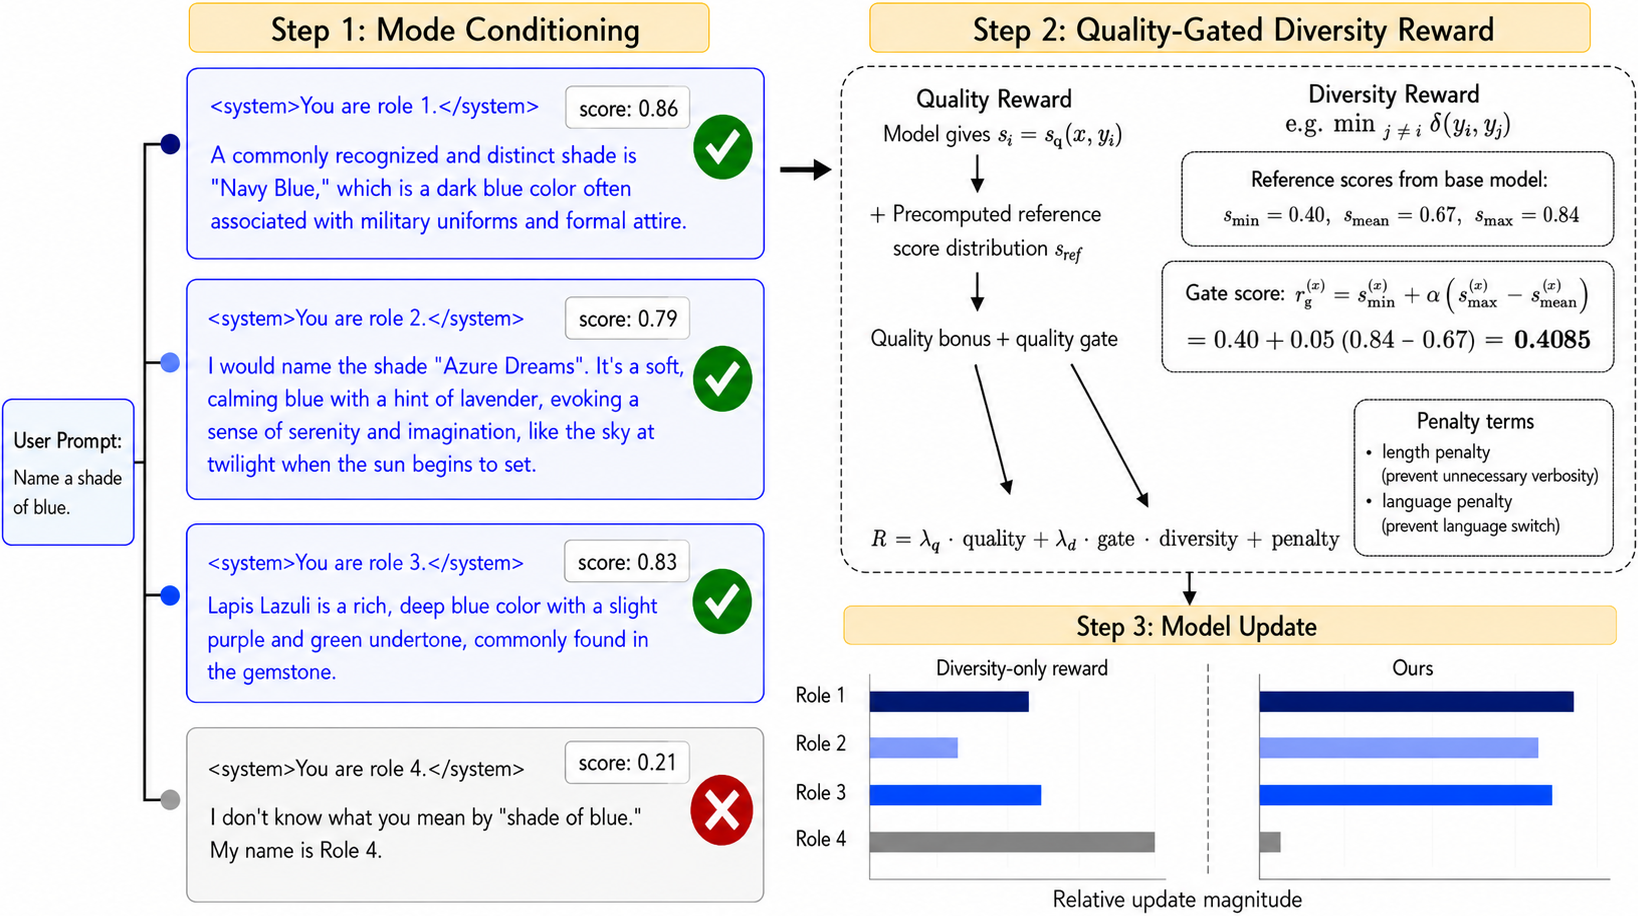
\includegraphics[width=\textwidth]{figures/method_v3.png}
        \label{fig:architecture}
    \end{subfigure}\hfill
    \begin{subfigure}[t]{0.2\linewidth}
        \centering
        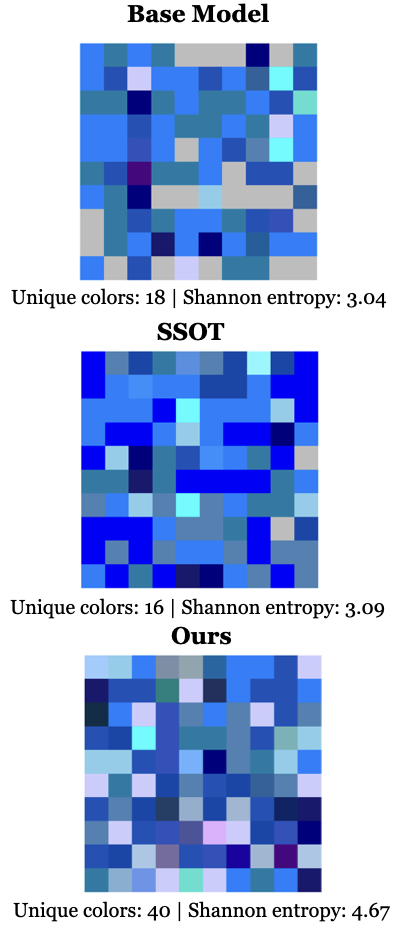
\includegraphics[width=\linewidth]{figures/blue.png}
        \label{fig:40blue}
    \end{subfigure}
    \vspace{-0.2cm}
\caption{\textbf{Left}: Overview of \method. \method{} uses mode conditioning to elicit diverse candidate responses, then applies a quality-gated diversity reward with penalty terms to promote high-quality diversity. Each candidate is labeled with its quality score $s_i$ relative to the prompt-adaptive quality threshold $\tau_q^{(x)}$. Candidates with $s_i<\tau_q^{(x)}$ have $g(x,y_i)=0$ and therefore receive no diversity credit. Step 3 shows the resulting signed group-relative advantages $\widehat{A}_i$; positive advantages promote a response, whereas negative advantages suppress it during the policy update. Matching colors track the same response through Steps 1--3. \textbf{Right}: 100 responses to the prompt \textbf{``Name a shade of blue''} from the Qwen3-8B initial policy (\texttt{Qwen/Qwen3-8B}), String Seed of Thought (\ssot)~\citep{Misaki2026}, and \method{} under diverse-mode inference. \method{} produces 40 distinct shades of blue, 122\% more than the Qwen3-8B initial policy and 150\% more than \ssot. \liweiaddressed{It's unclear what the two bar charts of Model update mean? I think the issue is that, it's not intuitive which of the four generations in Step 1 is considered low quality, and hence needs penalty. One possibility is to add in the quality score (mock-up is fine), to the upper-right corner of each generation box, plus, provide a reference score. So that it makes it more clear which response should be suppressed during model update. Also the four bars in Step 3 seem to have different colors compared to the four boxes in Step 1. }
}
\label{fig:moda + 40blue}
\end{figure*}


\section{Introduction}
\label{sec:introduction}

Post-training alignment is essential for improving the capability and safety of large language models (LLMs), but it also introduces a concerning side effect: \textit{mode collapse}. Aligned models increasingly favor a narrow set of responses (the ``mode'') over the broader space of plausible outputs, resulting in a substantial loss of generation diversity~\citep{jiang2025artificialhivemindopenendedhomogeneity, west2025base, huang2024self, sourati2026homogenizingeffectlargelanguage}. Yet in many domains, diversity is not merely desirable but essential. In AI-assisted scientific discovery, progress relies on exploring a broad and plausible hypothesis space rather than prematurely converging on a single line of inquiry~\citep{gruver2023proteindesignguideddiscrete, romera2024mathematical}. Likewise, generative diversity is critical for applications requiring creativity and open-ended exploration~\citep{Shumailov2024AIMC, abdulhai2026llmsdistortwrittenlanguage}. While inference-time interventions~\citep{Misaki2026, Zhang2025} can partially mitigate this loss of diversity, a more fundamental solution is to redesign post-training algorithms so that expressivity is preserved throughout the alignment process by construction.

We introduce \method~(\textbf{Mo}de-conditioned \textbf{D}iversity \textbf{A}lignment), an online post-training RL algorithm that jointly optimizes the quality and diversity of generated responses by formulating alignment through the lens of multi-agent reinforcement learning (MARL), where agents develop diverse behaviors through competition and coordination~\citep{eysenbach2018diversityneedlearningskills,liang2024learning,li2021celebratingdiversitysharedmultiagent}. \method{} introduces \textit{role conditioning} to instantiate multiple lightweight agents within a single shared policy. Specifically, we prepend abstract role tokens to the system prompt, enabling each role to generate a response to the same user query while independently optimizing a group-relative diversity reward. This creates competitive reward dynamics among roles, encouraging them to specialize in distinct regions of the high-quality response space and collectively produce a diverse set of outputs.

A key design choice of \method{} is a \textit{prompt-adaptive quality gate} that grants diversity rewards only to responses exceeding a prompt-specific quality threshold computed from a frozen reference policy. Among responses that satisfy the gate, diversity is rewarded according to semantic distance from the nearest neighboring response, encouraging exploration within the space of sufficiently high-quality generations. By coupling diversity rewards with quality, this mechanism prevents reward hacking, in which models maximize diversity by producing unusual but irrelevant outputs~\citep{li2025jointlyreinforcingdiversityquality,wan2025enhancingpersonalizedmultiturndialogue}.

Assessing quality-diversity tradeoffs requires evaluating both standard capabilities and applications that benefit from diverse outputs. To this end, we curate a comprehensive 11-task evaluation suite that jointly measures general capability retention and diversity-focused applications where multiple high-quality generations are useful or necessary. The suite includes seven general capability benchmarks (GSM8K, MMLU, GPQA, BoolQ, HellaSwag, TruthfulQA, and IFEval) and four open-ended domain application benchmarks spanning scientific ideation and creative writing such as HypoBench~\citep{liu2026hypobenchsystematicprincipledbenchmarking}, PreScience~\citep{Ajith2026}, NoveltyBench~\citep{zhang2025noveltybenchevaluatinglanguagemodels}, and a held-out split of Infinite-Chat~\citep{jiang2025artificialhivemindopenendedhomogeneity}. We evaluate output diversity using complementary metrics: \textit{semantic-level} (SBERT), \textit{entropy-level} (E-Vendi), and \textit{entailment-level} (a learned pairwise discriminator). Under the same thinking-disabled setting, \method{} improves SBERT diversity and E-Vendi by 155.5\% and 94.0\%, respectively, over the Qwen3-8B initial policy on the diversity-focused benchmark suite, while simultaneously increasing average pass@1 by 10.3 percentage points over the initial policy, and by 7.0 percentage points over the strongest DivPO baseline on general capability benchmarks.

Compared with prior diversity-oriented post-training methods~\citep{li2025jointlyreinforcingdiversityquality, lanchantin2025diverse, chung2025modifyinglargelanguagemodel, Chen2025PosttrainingLL, slocum2025diversepreferencelearningcapabilities, Puri2026}, \method{} conditions diversity on an explicit mode token rather than baking it unconditionally into the model. As a result, it naturally supports two inference modes: supplying mode tokens yields a diverse set of responses, while omitting them recovers the base model's standard behavior, preserving single-response capability. More broadly, we hope \method{} motivates future work that brings richer MARL principles into LLM post-training.





%Post-training alignment in large language models (LLMs), while essential for enhancing model capability and safety, reveals a concerning issue: mode collapse, whereby the model favors a narrow set of responses (the “mode”) over all plausible outputs, leading to significant reduction in diversity among generated responses~\citep{Jiang2025, west2025base, huang2024self,sourati2026homogenizingeffectlargelanguage}.
%VI: I made a small change here to break up the long sentence, tried to keep it close to the original
% \liwei{I'd suggest to only mention mode collapse and cite multiple works (the more the better, bc we want to generously acknowledge previous works) that touches upon this, including the hivemind paper. bc we're essentially solving mode collapse in a single model, and hivemind has broader implication around multiple models. mode collapse is also more well-known}\liwei{only lightly mention these negative downstream impact would be helpful, but not over-exaggerate} 


% Post-training alignment is essential for improving the capability and safety of large language models (LLMs), but introduces a concerning side effect: \textit{mode collapse}. Aligned models favor a narrow set of responses (the “mode”) over all plausible outputs, leading to a significant reduction in diversity among generated responses~\citep{jiang2025artificialhivemindopenendedhomogeneity, west2025base, huang2024self,sourati2026homogenizingeffectlargelanguage}. Yet across many domains, diversity is not merely desirable but necessary. In applying AI for scientific discovery, progress depends on exploring a broad and plausible hypothesis space rather than converging prematurely on a single line of inquiry~\citep{gruver2023proteindesignguideddiscrete, romera2024mathematical}. Similarly, generative diversity is also critical to tasks that require creativity and open-ended possibilities ~\citep{Shumailov2024AIMC, abdulhai2026llmsdistortwrittenlanguage}. 
% While inference-time interventions~\citep{Misaki2026, Zhang2025} can partially remedy diversity loss, a more fundamental solution is to rethink post-training methods so that expressivity is preserved by design throughout alignment.

% \liwei{I think we should only lightly mention these negative downstream impacts would be helpful. discussing this so much into the details feels a bit over-exaggerating, and pushes our true contributions to much later in the paper. We should always seek to say our contributions first.} 
%This motivates the need for a post-training alignment method that addresses the mode collapse issue without sacrificing the response quality. 
% \liwei{mention that while inference-time interventions [cite] can improve text diversity to a certain extent, it is equally important to rethink post-training methods so that expressivity is preserved by design throughout the alignment process itself.}

%Many useful applications of language models are not single-answer tasks. Brainstorming, scientific hypothesis generation, research planning, legal analysis, design critique, and creative writing often require a set of plausible responses that differ in assumptions, framing, evidence, or solution strategy. In these settings, a model that repeatedly produces the same reasonable answer can be less useful than a model that exposes several distinct but still high-quality alternatives.d

%Recent work suggests that this is a systematic limitation of current language models. Studies of open-ended generation find that models often collapse to similar outputs across repeated samples and even across different model families ~\citep{jiang2025artificialhivemind}. Other work argues that alignment and post-training can reduce conceptual diversity, even when they improve average helpfulness or safety ~\citep{murthy2025onefish}. NoveltyBench similarly shows that standard capability does not imply humanlike diversity: strong models can still fail to produce multiple meaningfully distinct, useful responses for prompts that admit many valid answers ~\citep{zhang2025noveltybench}.

% \liwei{the main issue with the current intro is that we introduce our contribution too late in the paragraph. We should start with a relatively short paragraph to describe the limitations of current methods, and concisely about the impacts, then in the second paragraph, directly jump into our contribution. We can then in the next paragraph, expand on what's the advantages of our method compared to previous methods. You can transition by saying something like "\method is in stark constract with previous approaches that xx, xx, but lack of xx, xx"}

%existing methods address diversity primarily at the lexical or shallow semantic level, and none provide a principled training-time mechanism that jointly optimizes for output quality and deep conceptual diversity across diverse application domains.

% \liwei{have the first sentence introducing what we build in this work. then move on to ground its design in motivations.}

% However, unconstrained diversity optimization is prone to reward hacking, where models generate unusual but irrelevant responses to maximize diversity rewards~\citep{li2025jointlyreinforcingdiversityquality,wan2025enhancingpersonalizedmultiturndialogue}. To address this, \method{} incorporates a \textbf{prompt-adaptive quality gate} that grants diversity rewards only to responses whose quality exceeds a prompt-specific threshold computed from a frozen reference policy. Among responses that pass the gate, diversity is rewarded according to semantic distance from the nearest neighboring response, encouraging exploration only within the space of sufficiently high-quality generations.


% We introduce \method~(\textbf{MO}de-conditioned \textbf{D}iversity \textbf{A}lignment), an online post-training RL algorithm that jointly optimizes response quality and diversity by formulating alignment through the lens of multi-agent reinforcement learning (MARL), where agents develop diverse behaviors through competition and coordination~\citep{eysenbach2018diversityneedlearningskills,liang2024learning,li2021celebratingdiversitysharedmultiagent}. \method{} instantiates multiple lightweight agents within a single shared policy via \textit{role conditioning}: abstract role tokens are prepended to the system prompt so that each role generates a response to the same query while optimizing a group-relative diversity reward, encouraging specialization into distinct regions of the high-quality response space. To prevent reward hacking, where models maximize diversity by producing unusual but irrelevant outputs~\citep{li2025jointlyreinforcingdiversityquality,wan2025enhancingpersonalizedmultiturndialogue}, \method{} incorporates a \textbf{prompt-adaptive quality gate} that grants diversity rewards only to responses exceeding a prompt-specific quality threshold computed from a frozen reference policy. Among responses that pass the gate, diversity is rewarded according to semantic distance from the nearest neighboring response, promoting exploration only within the space of sufficiently high-quality generations.

% However, unconstrained diversity optimization can be vulnerable to reward hacking, where the model produces unusual but irrelevant responses to maximize its diversity reward~\citep{li2025jointlyreinforcingdiversityquality,wan2025enhancingpersonalizedmultiturndialogue}. To ensure that diversity gains do not come at the expense of quality, \method{} incorporates a \textbf{prompt-adaptive quality gate} as a key design choice of its online RL reward. The gate assigns diversity credit only to responses whose quality score exceeds a precomputed prompt-specific reference threshold. Among responses that pass this gate, \method{} rewards semantic uniqueness based on the distance to the response's nearest neighbor within the group, thereby encouraging diversity only within the space of sufficiently high-quality generations.

% We present \method~(\textbf{MO}de-conditioned \textbf{D}iversity \textbf{A}lignment), a post-training alignment algorithm that jointly optimizes quality and diversity of generated responses. We draw inspiration from multi-agent reinforcement learning (MARL), where a rich body of work has explored how agents can develop diverse behaviors through competition and coordination~\citep{eysenbach2018diversityneedlearningskills,liang2024learning,li2021celebratingdiversitysharedmultiagent}. Transplanting this idea into the LLM setting, we treat each role as an independent agent competing to maximize the uniqueness of its response within the group, while preserving a quality objective. This naturally motivates our mode-conditioned post-training reinforcement learning framework which creates several agents within one policy by injecting abstract roles into the system prompt. During training, each role %acts as an independent agent and receives its own diversity reward, based on the uniqueness of its response compared to that of the other agents. 
% acts to independently optimize its diversity reward, introducing competitive, non-stationary reward dynamics. Collectively, this steers the model toward distinct regions of the response space, thereby generating a population of diverse outputs. 

% However, as with many RL post-training techniques, this setup is vulnerable to reward hacking, where the model can produce unusual but irrelevant responses to maximize its diversity reward \citep{li2025jointlyreinforcingdiversityquality, wan2025enhancingpersonalizedmultiturndialogue}. \liwei{I feel we can merge the previous and this paragraph to introduce the algorithm all at once, without needing to have a seperate paragraph for quality gate itself. A possible narrative (need polishing and plugging in actual sentences): We preset MODA. As motivated by MARL, we introduce role-conditioning to allow multi-agent competition and coordination to unleash more diverse model behavior. To ensure that quality does not get impaired by increasing diversity, we further introduce quality gate.}
% To mitigate this, we design
% % \liwei{I think we don't need an acronym for the reward. it's rather distracting and hard to remember}, 
% a prompt-adaptive reward that jointly ensures response quality and diversity: %by gating the response quality: 
% \textit{Quality Gated Diversity Reward}. This technique %{\method} 
% ensures diversity does not come at the expense of quality, by only rewarding the diversity of responses above a precomputed target reference  quality score. Thus only sufficiently high-quality responses are rewarded for diversity, specifically for their uniqueness within the response group, based on the distance to the response's semantic nearest neighbor. \liwei{I strongly suggest to frame quality gate as a "key design choice" of the overall online RL algorithm centered on role-conditioning. Right now, we put a lot of emphasis on the quality-gate, almost as a separate contribution. This has two downsides: (1) making our full algorithm contribution look less integral, with only the role-conditioned component introduced at the time of introducing the algorithm, (2) call too much attention to the quality-gate itself as an independent technical component, which dilute the overall contribution.}

% We curate a comprehensive 11-task evaluation suite that measures general capability retention and domain application \liwei{domain applications that benefit from or require diverse model generations, give examples of the benchmarks to give a concrete sense of the evaluation scope. the word "domain application" is in particular vague}, covering output diversity across complementary metrics spanning semantics and concepts. We select application domains with real-world significance, including scientific reasoning and creative expression. The resulting model achieves \textbf{29.0\%} and \textbf{47.3\%} improvement in relation to the Qwen3-8B initial policy under the same no-thinking setting, %\liwei{improving in relation to what? also should mention improvement in relation to other baselines too.} 



% \liweiaddressed{We should mention a little more of how our method is comparing to previous baselines, either inference-time or training-time baselines. Without mentioning any baselines at all makes our work sounds less grounded, because this direction itself is well-known to already have several solutions.}

%By properly re-designing the post-training algorithm, 

% \liweiaddressed{The last paragraph is a bit redundant and disorganized. Try to sharpen and tighten the language.}
%\method~ presents a new alternative to post-training that retains quality and diversity simultaneously, shedding light on an alternative paradigm of multi-objective optimization in LLM post-training through MARL-inspired mode conditioning. Previous works use MARL to simulate or coordinate LLM-based agents \citep{Wang_2024, du2023improvingfactualityreasoninglanguage, liuevaluating}, while our results suggest that ideas can be adapted to language-model training.

%We hope \method{} encourages future work that imports richer MARL principles into LLM training. In \method{}, role-conditioned modes serve as lightweight agents within a single shared policy: each mode explores a different region of the response space, receiving its own group-relative learning signal. This turns diversity generation into a coordination problem, where the goal is not only to improve individual responses, but also to shape the population of responses. More importantly, mode conditioning provides explicit surfaces to accommodate divergent mode seeking behaviors while sharing a common policy.

% \liwei{add a final paragraph to highlight broader impact and most important takeaway from our work. something like, we found that by properly re-design post-training algorithm that accommodate quality and diversity simultaneously, we achieve a Pareto frontier between Q an D, shedding light on ......}

%Our key insight is that diversity can be treated as a reward signal during RL: by injecting a mode-conditioning token into the system prompt, we steer the model toward distinct regions of the output space, and reward responses that are both high-quality and meaningfully different from other responses generated for the same prompt. The resulting model achieves [X]\% improvement in diversity over [BASELINE] while maintaining [QUALITY METRIC] within [Y]\% of the base model, demonstrating that quality and diversity need not trade off. We validate this across three application domains, including scientific hypothesis generation, creative writing, and mathematical proof, showing consistent gains in each.

% \liwei{I would suggest to remove the itemized contribution listing, but rather integrate them in the narrative of the intro. Also, the alignment method and the reward function should not be treated as separate contributions. they should be introduced together as different part of the overall \method. also again, we should not oversell the benchmark contribution, because we are mostly repurposing previous works.}

%Our contributions include:\textbf{Alignment Method: \method}: a post-training alignment method by encouraging inter-agent diversity through mode-conditioned reinforcement learning under diverse mode, while retaining its general capability under standard mode.\textbf{Reward Function: \qgdr}: a prompt-adaptive reward function that jointly optimizes quality and diversity of generated responses. \textbf{Evaluation Suite: \bench:} a comprehensive evaluation suite that measures general capability retention and domain application, covering output diversity across complementary metrics spanning semantics and concepts, with application domains chosen for their real-world significance, including scientific reasoning and creative expression.

%A simple way to seek diversity is to sample repeatedly with nonzero temperature, prompt the model with different personas, or ask it to avoid previous answers. These methods can help, but they are inference-time interventions rather than learned specialization. Prompt-only methods such as String Seed of Thought (SSoT) go further by asking the model to generate an internal random string and use it as a seed for probabilistic or diverse generation ~\citep{misaki2025ssot}. This supports the broader idea that language models can expose more varied behavior when given an explicit control variable, but it does not train the model to make that control variable stable, high-quality, or semantically separated across roles.

%We study whether a single shared language model can be post-trained to expose multiple controllable modes of behavior. The model is conditioned on abstract numbered role codes, such as \texttt{role\_1}, \texttt{role\_2}, and so on. Each role is trained to produce responses that remain useful while being semantically distinct from the responses produced by the other roles for the same prompt. The role code therefore functions as a learned internal seed: at inference time, querying several roles yields a set of diverse candidate answers, while omitting the role code should preserve ordinary instruction-following behavior.

%This paper focuses on open-ended and scientific generation, where diversity is directly useful. We evaluate on NoveltyBench, Infinite-Chat, and HypoBench, and we separately test capability retention in no-role mode to ensure that diversity training does not make the model worse at ordinary closed-form tasks.





% \newpage

\section{Related work}
\label{sec:related_work}

\paragraph{Why Does Generation Diversity Matter?}
Language models often collapse toward a narrow set of high-probability responses, resulting in an ``Artificial Hivemind'' characterized by substantial intra- and inter-model homogeneity on open-ended prompts \cite{jiang2025artificialhivemindopenendedhomogeneity}. Zhang et al.~\cite{Zhang2025} further show that post-training alignment reduces diversity through biases in preference data, limiting performance in domains that require diverse outputs.
In scientific reasoning, automated research agents benefit from a wider exploration breadth \citep{zou2026fmlbenchbenchmarkingmachinelearning}, and mode collapse causes reduced exploration in solution spaces \citep{yuan2026agenticredevolvingagenticsystems}. In creative tasks, reduced diversity in LLM outputs also diminishes the creativity of LLM-assisted writing \citep{abdulhai2026llmsdistortwrittenlanguage,Anderson2024HomogenizationEO,padmakumar2023does}. In mathematical proofs, strategy diversity is critical for exploring distinct reasoning paths \citep{Wu2025, Cao2025TowardsAM}. These findings motivate methods that preserve quality while expanding the range of model outputs.

% Language models often collapse toward a narrow set of high-probability responses. Jiang et al.~\cite{jiang2025artificialhivemindopenendedhomogeneity} characterize this as an ``Artificial Hivemind,'' demonstrating substantial intra- and inter-model homogeneity on open-ended prompts, while Zhang et al.~\cite{Zhang2025} show that post-training alignment further amplifies this effect through biases in preference data. This lack of diversity is particularly problematic in domains requiring broad exploration. Diverse outputs improve exploration in scientific reasoning and research agents \citep{Zou2025, yuan2026agenticredevolvingagenticsystems}, enhance creativity in LLM-assisted writing \citep{abdulhai2026llmsdistortwrittenlanguage,Anderson_2024,padmakumar2023does}, and increase the effectiveness of repeated sampling for mathematical reasoning by exploring distinct proof strategies \citep{Wu2025, Cao2025TowardsAM}. These findings motivate methods that preserve quality while expanding the diversity of model outputs.

\paragraph{Measuring Diversity of LLMs.}
Diversity of LLM-generated content has been measured along several dimensions. Lexical metrics include distinct n-grams \citep{ippolito2019comparison}, Self-BLEU \citep{zhu2018texygen}, Measure of Textual Lexical Diversity (MTLD) \citep{McCarthy2010MTLDVA}, and compression-based homogeneity scores \citep{shaib2024standardizing}. Semantic metrics build on sentence embeddings \citep{reimers2019sentencebertsentenceembeddingsusing, wieting2018paranmt} and information-theoretic constructions such as the Vendi Score \citep{friedman2023vendiscorediversityevaluation} and its conditional variant \citep{jalali2024conditionalvendiscoreinformationtheoretic}, as well as gradient-based measures like G-Vendi \citep{jung2025prismaticsynthesisgradientbaseddata}. A complementary line of work studies how diversity collapses through the training pipeline \citep{kirk2024understandingeffectsrlhfllm, omahony2024attributingmodecollapsefinetuning, padmakumar2023does, west2025base, dang2025assessing}, and recent benchmarks evaluate humanlike or effective semantic diversity directly \citep{zhang2025noveltybenchevaluatinglanguagemodels, shypula2025evaluatingdiversityqualityllm, guo2025benchmarking, Shahid2025}. However, most evaluations assess diversity or quality in isolation, whereas we jointly evaluate capability and diversity across real-world applications to ensure models preserve multiple plausible answers without mode collapse \citep{Misaki2026,Puri2026} or catastrophic forgetting \citep{luo2025empiricalstudycatastrophicforgetting}.



% \liwei{Can we tighten the following paragraph a bit more? It's a bit too long.}
\paragraph{Improving Diversity during Training and Inference.}
Recent work has explored improving diversity through prompting \citep{Zhang2025, lau2025dipperdiversitypromptsproducing, lagzian2025multinoveltyimprovediversitynovelty, wang2025multilingualpromptingimprovingllm, Kim2026, Wu2025}, decoding \citep{holtzman2020curiouscaseneuraltext, nguyen2024turningheatminpsampling, ruan-etal-2025-g2, wang2024lpoadaptivedecodinglatent}, and training \citep{li2025jointlyreinforcingdiversityquality, lanchantin2025diverse, chung2025modifyinglargelanguagemodel, Chen2025PosttrainingLL, slocum2025diversepreferencelearningcapabilities, Puri2026} (see Appendix~\ref{appx:related-work-table} for a comparison table). At inference time, Verbalized Sampling \citep{Zhang2025} prompts models to express a distribution over possible responses, while String Seed of Thought \citep{Misaki2026} injects random strings as entropy sources. DIPPER \citep{lau2025dipperdiversitypromptsproducing} and Multi-Novelty \citep{lagzian2025multinoveltyimprovediversitynovelty} construct diverse prompt ensembles, and multilingual, persona, or chain-of-thought prompting can elicit variations \citep{wang2025multilingualpromptingimprovingllm, Wu2025}. At decoding time, min-$p$ sampling \citep{nguyen2024turningheatminpsampling} adaptively truncates low-probability tokens based on model confidence, while G2 \citep{ruan-etal-2025-g2} and adaptive temperature methods \citep{wang2024lpoadaptivedecodinglatent} guide generation with auxiliary diversity modules or learned per-instance decoding parameters. In post-training, RL has emerged as a powerful method for enhancing diversity. Multi-answer RL \citep{Puri2026} trains models to output multiple diverse answers within one response; Soft Preference Learning decouples entropy from KL-penalty to improve lexical and semantic variety \citep{slocum2025diversepreferencelearningcapabilities}; DivPO \citep{lanchantin2025diverse} applies DPO to responses that are both diverse and high quality. 

Several recent works share our goal of jointly optimizing quality and diversity through RL. DARLING \citep{li2025jointlyreinforcingdiversityquality} balances quality and diversity by rewarding a multiplicative aggregation of quality and diversity metrics; DQO \citep{Chen2025PosttrainingLL} uses a determinant-based group diversity reward, but assigns the same reward to all responses in the group. GRPO-Unlikeliness \citep{he2025rewardingunlikelyliftinggrpo} and GAPO \citep{anschel2025group} both encourage diversity through frequency- and likelihood-based rewards. However, although these methods explore different reward designs, none of them allow a single model to switch between producing one high-quality answer and a diverse set of responses.
\method, on the other hand, approaches quality-diversity alignment from a MARL-inspired perspective, treating diverse generation as a competition-and-coordination problem among role-conditioned agents within a shared policy. This formulation enables explicit per-role credit assignment under quality constraints, encouraging specialization across the high-quality response space while keep the model's standard behavior intact. 
% \begin{figure}[t!]
    \centering
    \begin{subfigure}[t]{0.78\linewidth}
        \centering
        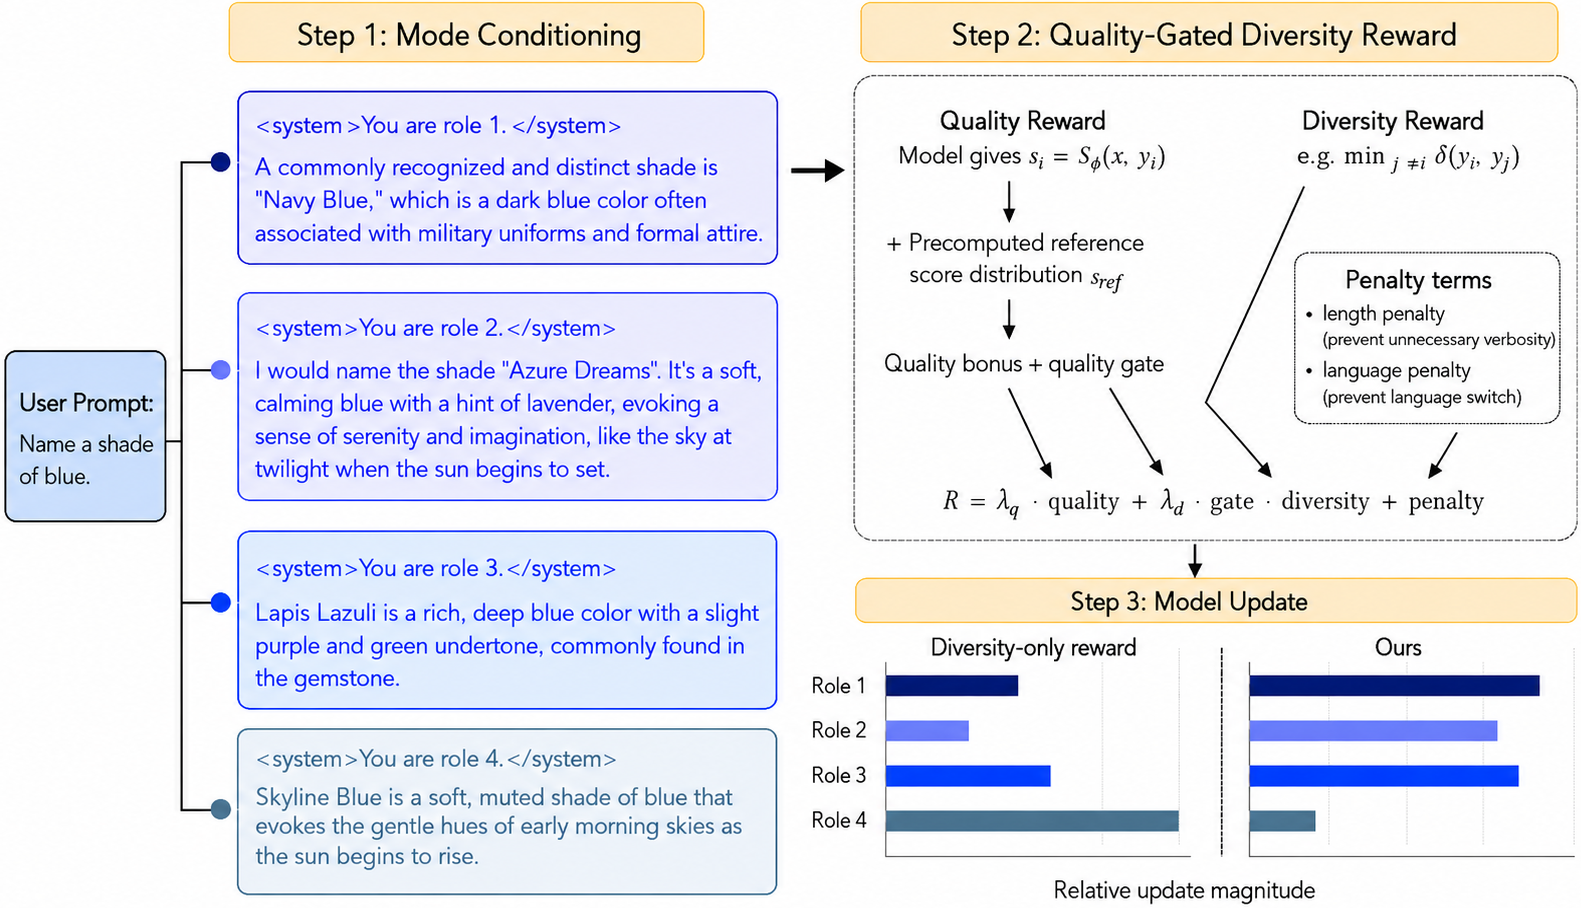
\includegraphics[width=\textwidth]{figures/method_v2.png}
        \label{fig:architecture}
    \end{subfigure}\hfill
    \begin{subfigure}[t]{0.2\linewidth}
        \centering
        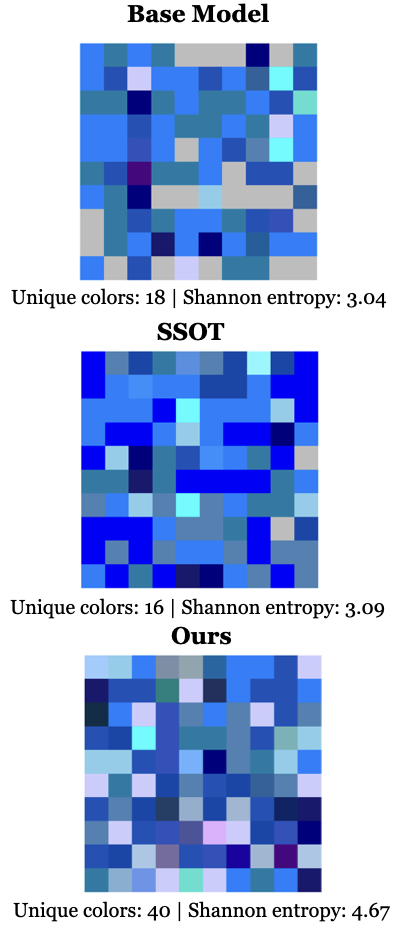
\includegraphics[width=\linewidth]{figures/blue.png}
        \label{fig:40blue}
    \end{subfigure}
    \vspace{-0.2cm}
\caption{Left: Overview of \method. \method~uses mode conditioning to elicit diverse candidate responses, then applies a quality gated diversity reward with penalty terms to promote high-quality diversity while suppressing low-quality or reward-hacking outputs. Right: 100 responses to the prompt \textbf{`Name a shade of blue''} from Qwen-3-8B (base), \ssot, and \method~under diverse mode inference. \method~produces 40 distinct shades of blue, 122\% more than the base model and 150\% more than \ssot, with 100\% valid answers, versus 20\% invalid answers from the base model. 
}
\label{fig:moda + 40blue}
\end{figure}

\section{Preliminaries: LLM Alignment with Reinforcement Learning}

% \liwei{talk about preliminary of LLM alignment with GRPO. And mention why it induce mode collapse -- bc it only incentivize the model to seek the highest reward region, without flexibility to accommodate more high reward outcomes.}

% \liwei{move the intro of reward to the next section}
Let $\mathcal{S}$ denote the set of natural language token sequences.
A language model $\pi(\cdot \mid x)$ takes a prompt $x \in \mathcal{S}$ as input and outputs a probability distribution over $\mathcal{S}$.
We denote the probability of a specific response $y \in \mathcal{S}$ as $\pi(y \mid x)$.
Given a prompt $x$, we sample $k$ independent responses
$\{y_1, y_2, \ldots, y_k\} \sim \pi(\cdot \mid x)$,
forming a \textit{response group} $\mathcal{Y} = \{y_i\}_{i=1}^{k}$. While RL post-training on LLMs demonstrates strong empirical results in enhancing reasoning capability\citep{shao2024deepseekmath, Guo_2025}, it is known to suffer from mode collapse. Conventional RL post-training only incentivizes the model to seek the highest reward region, without flexibility to accommodate more diverse responses. Our goal is to optimize the policy so that the generated responses are not only high-quality, but also diverse, creative, and non-redundant. 

%We therefore introduce \textbf{Quality-Gated Diversity Reward} which jointly values \textit{quality} and \textit{diversity} within the response group $\mathcal{Y}$ by gating the diversity term by quality to prevent the model from being rewarded for producing unusual but degenerate responses, described in Section \ref{subsec:qgdr}

% \liwei{this section is too short and hence a bit weird to keep it an independent section. can we fold it into current section 4, as the first subsection?}

\section{\methodcolor: Mode-Conditioned Diversity Alignment for LLMs}
\label{sec:method}

\subsection{Preliminaries: LLM RL Post-Training and Mode Collapse}
\label{ssec:preliminaries}

Recent RL post-training has substantially improved the utility and safety of LLMs \citep{shao2024deepseekmath,Guo_2025}. However, optimizing only the expected reward often leads to \emph{mode collapse}, where the learned policy focuses on a small set of high-reward responses while suppressing equally valid alternatives \citep{kirk2024understandingeffectsrlhfllm}. As a result, generated responses become repetitive despite maintaining high quality. \textbf{Our goal is to learn policies that generate responses that are simultaneously high-quality, diverse, and non-redundant.}

Let $\mathcal{S}$ denote the space of natural language token sequences. Given a prompt $x \in \mathcal{S}$, a language model $\pi(\cdot \mid x)$ defines a probability distribution over responses in $\mathcal{S}$, where $\pi(y \mid x)$ denotes the probability of generating response $y \in \mathcal{S}$. For each prompt, we independently sample $k$ responses, $y_1, \ldots, y_k \sim \pi(\cdot \mid x)$, forming a \emph{response group} $\mathcal{Y}=\{y_i\}_{i=1}^{k}$.

Conventional RL post-training maximizes the expected reward $\max_{\theta} J_{\mathrm{RL}}(\theta) = \mathbb{E}_{x \sim \mathcal{D}}\left[\mathbb{E}_{y \sim \pi_{\theta}(\cdot \mid x)} r(x,y)\right]$, where $r(x,y)$ is the reward assigned to response $y$ for prompt $x$. Optimizing this objective alone progressively concentrates the policy on a small set of high-reward responses, reducing the policy entropy $H(\pi_{\theta}(\cdot \mid x)) = -\sum_{y \in \mathcal{S}} \pi_{\theta}(y \mid x) \log \pi_{\theta}(y \mid x)$ and causing the model to repeatedly generate only a few dominant responses despite the existence of many alternatives with comparable rewards. We refer to this phenomenon as \emph{mode collapse}.


\subsection{Multi-Agent Reinforcement Learning (MARL)-Inspired Mode Conditioning}

\paragraph{MARL Motivation.} Classical MARL studies how populations of agents can learn complementary behaviors by explicitly encouraging behavioral diversity through mechanisms such as information sharing, skill specialization, KL divergence maximization, and adversarial objectives \citep{eysenbach2018diversityneedlearningskills, liang2024learning, li2021celebratingdiversitysharedmultiagent}. We bring this perspective to LLM post-training by introducing \textit{mode conditioning}, where a single policy is conditioned on different role tokens and each role is treated as an abstract agent. Agents must learn how to produce responses that are unlike those of the other agents, introducing competitive dynamics that drive the agents to continually diversify their responses. Unlike standard alignment, mode conditioning provides a \textit{richer interface} that enables the model to internalize multiple high-quality behavioral modes.

\paragraph{Mode Conditioning via System Role Identifiers.} We instantiate mode conditioning by prepending role identifiers into the system prompt. In our primary setting, we adopt an intentionally minimal identity-based conditioning: \texttt{You are role $i$}. We use numbered roles instead of hand-crafted personas to avoid injecting domain-specific assumptions about desirable perspectives. Although our ablations show that crafted personas (e.g., ``innovative thinker,'' ``passionate educator,'' or ``methodical experimenter'') and token-based conditioning (e.g. ``Start with your response with APPLE / BANANA / ORANGE.") are also effective, we adopt the minimal identity-based conditioning to encourage emergent specialization.

Formally, let $x \in \mathcal{X}$ denote a user prompt and $\mathcal{Z}={z_1,\ldots,z_N}$ a fixed set of role identifiers. A shared policy $\pi_\theta(y\mid z_i, x)$ is conditioned on role $z_i$, with all roles sharing parameters $\theta$. During training, each role generates one response for $K$ prompts within the batch, forming a response group $\mathcal{Y}_x=\{y_{i,k}: i=1,\ldots,N; k=1,\ldots,K\}$. Each response receives a Quality-Gated Diversity Reward (\S~\ref{subsec:qgdr}), and the shared policy is optimized with Group Relative Policy Optimization (GRPO; \citep{shao2024deepseekmath}). Algorithm~\ref{alg: moda short} summarizes the training procedure.

\paragraph{Dual Inference Settings.} \label{sec:inference_modes} Not all prompts benefit from diverse responses. For example, factual queries such as ``\textit{What is Albert Einstein's birthday?}'' have a single correct answer. A key advantage of mode conditioning is that omitting the role instruction recovers the model's standard behavior, allowing \method{} to support both inference modes. Under the \textbf{standard mode}, the model generates a single response without a role identifier. Under the \textbf{diverse mode}, we prompt the model under multiple role identifiers to produce a candidate set ${y_1,\ldots,y_N}$. The resulting set can be returned directly, ranked by a quality model, or aggregated by a downstream model into a final answer.


\subsection{Quality-Gated Diversity Reward}
\label{subsec:qgdr}

Preserving quality while increasing diversity is critical: a diversity-only objective is vulnerable to reward hacking; it can be exploited by irrelevant, malformed, unnecessarily verbose, or superficially different responses. We therefore optimize a four-component reward consisting of a quality reward, a prompt-adaptive quality gate, a response-level diversity score, and explicit reward-hacking penalties:
\begin{equation}
\begin{aligned}
r_i
={}&
\underbrace{\lambda_q r_{\mathrm{qual}}(x,y_i)}_{\text{quality reward}}
+
\underbrace{\lambda_d g(x,y_i)}_{\text{quality gate}}
\underbrace{d(x,y_i,\mathcal{Y})}_{\text{diversity reward}} \\
&+
\underbrace{
r_{\mathrm{len}}(y_i)
+r_{\mathrm{lang}}(x,y_i)
+r_{\mathrm{fmt}}(y_i)
}_{\text{penalties}} .
\end{aligned}
\label{eq:qgdr}
\end{equation}

\paragraph{Prompt-Adaptive Quality Scoring.}
To determine whether our training preserves the original model's capability, we need a reference baseline: how the initial policy perform on the same prompt. To instantiate this baseline, for each prompt $x$, we score five responses sampled from the frozen initial policy and denote their minimum, mean, and maximum scores by $s_{\min}^{(x)}$, $\bar{s}^{(x)}$, and $s_{\max}^{(x)}$. Let $s_i=S_\phi(x,y_i)$ be the reference score assigned by the reward model. We define the prompt-adaptive threshold  $\tau_q$ and quality reward magnitude factor $\sigma_q$ as
\begin{equation}
    \tau_q^{(x)} = s_{\min}^{(x)} + \alpha \bigl(s_{\max}^{(x)} - \bar{s}^{(x)}\bigr),
    \qquad
    \sigma_q^{(x)} = \gamma \bigl(\bar{s}^{(x)} - s_{\min}^{(x)} + \epsilon\bigr),
\end{equation}
where $\alpha$ shifts the quality threshold above the reference minimum by a fraction of the reference score spread, $\gamma$ controls the sharpness of the scoring transition, and $\epsilon > 0$ ensures numerical stability.

The \textbf{binary quality gate} and\textbf{ quality reward}  for a generated response $y_i$ are
\begin{equation}
g(x, y_i) = \mathbf{1}\!\left[s_i \geq \tau_q^{(x)}\right]
,
\quad
    r_{\mathrm{qual}}(x, y_i)
    =
    \mu \tanh\!\left(
    \frac{s_i - \tau_q^{(x)}}{\sigma_q^{(x)}}
    \right)
\end{equation}
where $\mu$ controls the magnitude of the quality reward. This quality gate ensures that the model receives diversity reward only when the response meets the prompt-adaptive quality threshold $\tau_q^{(x)}$. As a result, responses that are merely more unusual, off-topic, or malformed compared to the initial policy would not receive diversity credit, preventing spurious solutions which hack the diversity reward.
Meanwhile, the quality reward ensures that responses above the threshold receive a positive bonus, while responses below the prompt-adaptive threshold still receive a quality-learning signal but receive no diversity credit. The bounded $\tanh$ transformation prevents the quality term from dominating optimization once the response already exceeds the threshold by a large margin. 

\paragraph{Diversity Scoring.}
For each prompt, the response group 
$\mathcal{Y}=\{y_1,\ldots,y_6\}$ contains one candidate from each of the six modes and best fits on 4 GPUs: one for the reward model and three for inference. We embed the final answer text using
\texttt{sentence-transformers/all-MiniLM-L6-v2}~\citep{wang2020minilmdeepselfattentiondistillation}.
% and $\ell_2$-normalize the resulting 384-dimensional embeddings:
% \begin{equation}
% \mathbf{e}_i
% =
% \frac{E_{\mathrm{SBERT}}(y_i)}
% {\lVert E_{\mathrm{SBERT}}(y_i)\rVert_2}.
% \end{equation}

The diversity reward directly optimized during training is the normalized semantic distance to the closest alternative within the response group:
\begin{equation}
d(x,y_i,\mathcal{Y})
=
\min_{j\neq i}
\frac{1-\mathbf{e}_i^\top\mathbf{e}_j}{2}.
\label{eq:training-sbert-diversity}
\end{equation}
Here, $y_i$ and every $y_j$ are responses to the same prompt but are generated under different roles, and each response is therefore compared with the other five candidates in its group. For thinking-enabled models, the hidden thinking trace is removed before embedding. This nearest-neighbor formulation rewards a response only if it is sufficiently distinct from its closest alternative, preventing multiple responses from collapsing to the same mode while a single outlier dominates the group-level diversity score. Consequently, role-conditioned agents are incentivized to specialize in different regions of the response space. Although we use semantic distance by default, the framework is agnostic to the diversity metric, and lexical, syntactic, or learned semantic measures can be substituted directly.

\paragraph{Reward-Hacking Penalties.}
The terms $r_{\mathrm{len}}$, $r_{\mathrm{lang}}$, and $r_{\mathrm{fmt}}$ are non-positive penalties for excessive length, language mismatch, and formatting or role-label leakage, respectively. These terms suppress superficial ways of increasing measured diversity without improving the usefulness of the response.

We optimize the shared policy via Group Relative Policy Optimization (GRPO)~\citep{shao2024deepseekmath}, estimating advantages from within-group reward comparisons over the role-conditioned response set without a separate value network. The full training objective is provided in Appendix~\ref{subsec:policy_optimization}.

\begin{algorithm}
\caption{\textsc{MoDA}: \textbf{Mo}de-Conditioned \textbf{D}iversity \textbf{A}lignment }
\label{alg: moda-stage2}
\small
\begin{algorithmic}[1]
\Require Dataset $\mathcal{D}$ with precomputed $(s_{\min},s_{\max},\mu_{\rm ref})$; policy $\pi_\theta$; reference policy $\pi_{\rm ref}$; reward model $S_\phi$; abstract roles $\mathcal{M}=\{m_i\}_{i=1}^N$; diversity metric $\delta$; weights $\lambda_q,\lambda_d$; constants $\alpha,\gamma,\epsilon,\eta$
\For{training iteration $t=1,\ldots,T$}
    \State Sample minibatch $\mathcal{B}\subset\mathcal{D}$
    \ForAll{$x\in\mathcal{B}$}
        \State Retrieve $(s_{\min}(x),s_{\max}(x),\mu_{\rm ref}(x))$
        \State $\tau_q^{(x)}\gets s_{\min}+\alpha(s_{\max}-\mu_{\rm ref})$,\quad
        $ \sigma_q^{(x)}\gets \gamma(\mu_{\rm ref}-s_{\min}+\epsilon)$
        \State Generate mode-conditioned responses with abstract roles
        $\mathcal{Y}(x)=\{y_i\sim\pi_\theta(\cdot\mid x,m_i)\}_{i=1}^N$
        \For{$i=1,\ldots,N$}
            \State $q_i\gets S_\phi(x,y_i)$ \quad \# Reward model assess response $y_i$
            \quad
            \State $R_{\rm quality}\gets \mu\tanh\!\left((q_i- \tau_q^{(x)})/ \sigma_q^{(x)}\right)$ \quad \# Compute quality bonus
            \State $G_{\rm qual}\gets \mathbf{1}\{q_i\ge  \tau_q^{(x)}\}$,\quad
            $R_{\rm div}\gets \min_{j\ne i}\delta(y_i,y_j)$ \# Quality gate and diversity reward
            \State $R_i\gets \lambda_q R_{\rm qual}
            +\lambda_d G_{\rm qual}R_{\rm div}
            +R_{\rm penalty}(x,y_i)$
        \EndFor
        \State $A_i\gets \bigl(R_i-\mathrm{mean}(R_{1:N})\bigr)/
        \bigl(\mathrm{std}(R_{1:N})+\eta\bigr)$ for $i=1,\ldots,N$
    \EndFor
    \State Update $\pi_\theta$ with GRPO using advantages $\{A_i\}$ and KL regularization to $\pi_{\rm ref}$
\EndFor
\State \Return trained policy $\pi_\theta$
\end{algorithmic}
\label{alg: moda short}
\end{algorithm}

% \liwei{While our goal is to improve the model's ability to generate diverse responses to the same prompt, quality is a non-sacrificeable bottom-line. To achieve the Pareto frontier between quality and diversity, we introduce ....} 
%Prior work such as DivPO \cite{lanchantin2025diverse} has used quality thresholds to gate diversity selection in its preference pair construction in an offline DPO setting, we adapt this principle to the online RL setting with a prompt-adaptive formulation.
%Standard reward functions score each response $y_i$ in isolation via a scalar quality signal $s_i = S_\phi(x, y_i) \in \mathbb{R}$, ignoring inter-response relationships. We instead define a group-level reward, which jointly values \textit{quality} and \textit{diversity} within the response group $\mathcal{Y}$. 

% \paragraph{Reference score instantiations.}
% For each prompt $x$, we sample five responses from the base model and score each response using the reward model $S_\phi$. The resulting scores define a prompt-adaptive reference quality distribution, summarized by $s_{\min}^{(x)}$, $s_{\max}^{(x)}$, and $\bar{s}^{(x)}$. This reference distribution serves as a calibration baseline for comparing the quality scores of responses generated by the trained policy.

% \paragraph{Reward-hacking penalty.}
% In preliminary experiments, we observed that the algorithm maximizes its diversity reward by engaging in language mixing and producing longer responses, a phenomenon also observed by DeepSeek-R1\citep{Guo_2025}. The penalty term is thus designed to suppress degenerate reward-hacking behaviors that can artificially increase measured diversity without improving response usefulness. Specifically, we include penalties for excessive length and language mismatch.% The additive structure of QGDR allows quality to remain an active training signal for all responses, while the quality gate prevents the diversity term from being activated unless the response is sufficiently useful.



% \begin{figure*}[t!]
%     \centering
%     \begin{subfigure}[t]{0.78\linewidth}
%         \centering
%         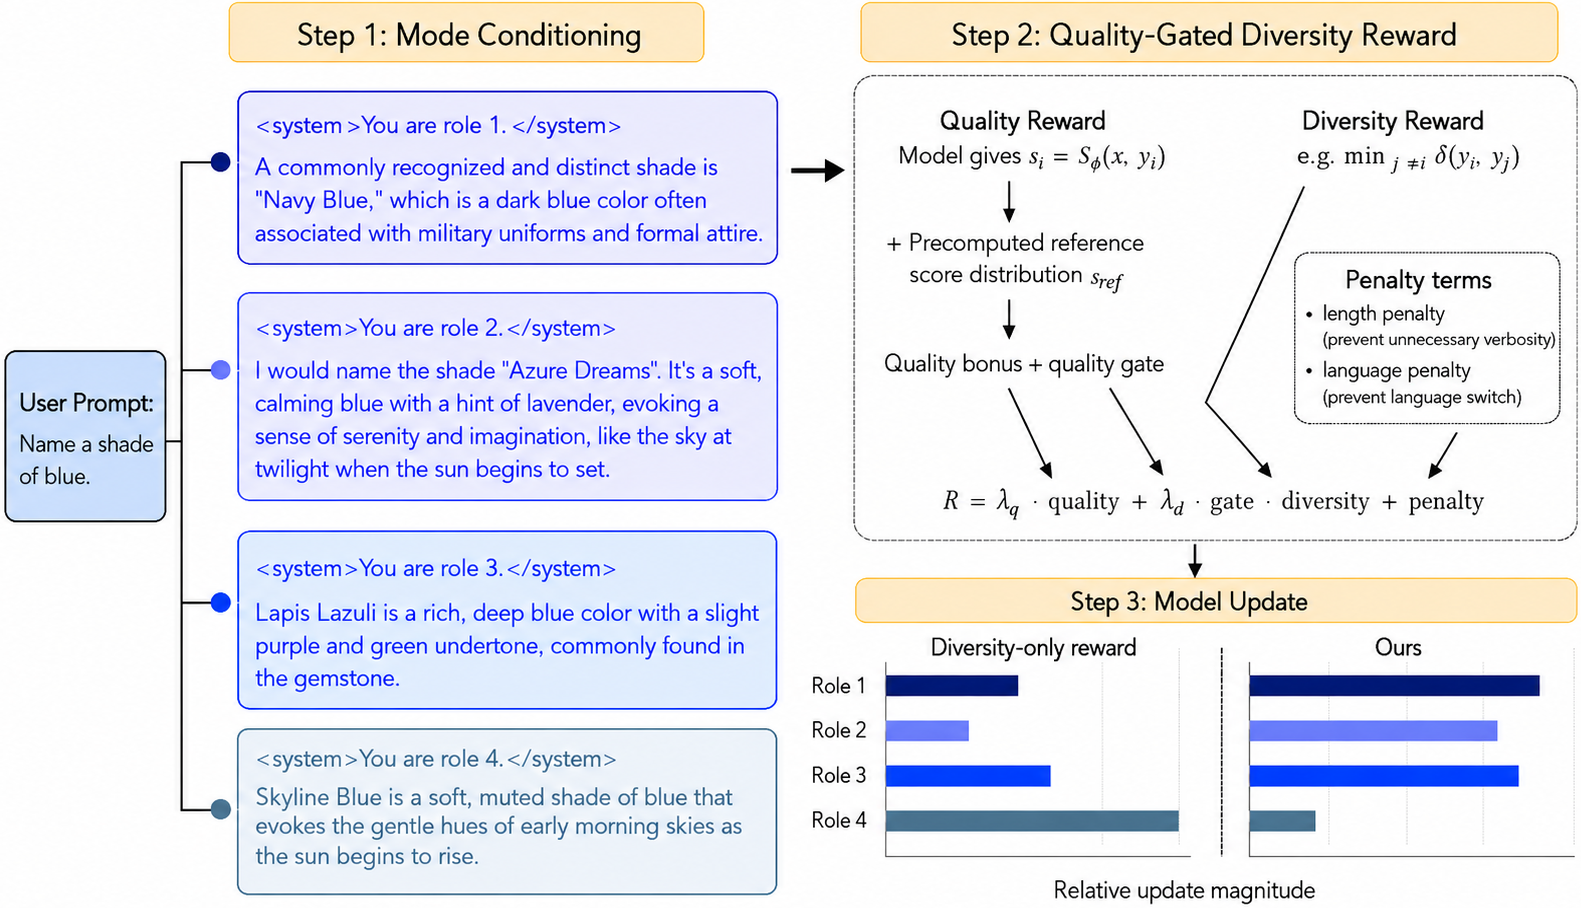
\includegraphics[width=\textwidth]{figures/method_v2.png}
%         \label{fig:architecture}
%     \end{subfigure}\hfill
%     \begin{subfigure}[t]{0.2\linewidth}
%         \centering
%         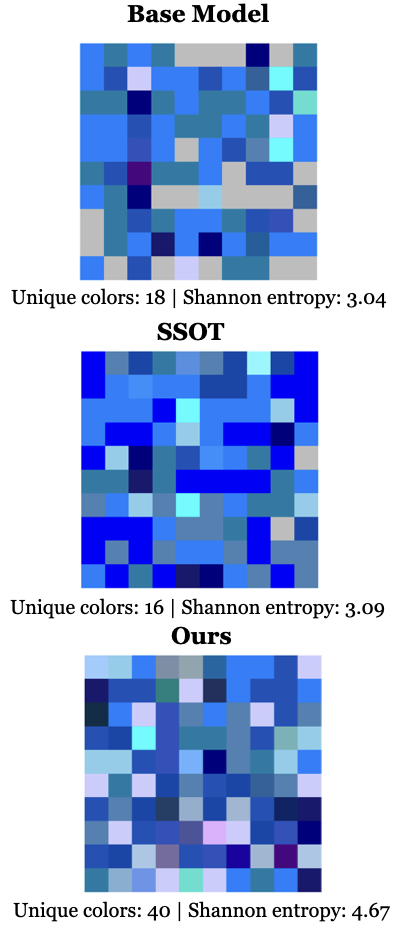
\includegraphics[width=\linewidth]{figures/blue.png}
%         \label{fig:40blue}
%     \end{subfigure}
%     \vspace{-0.2cm}
% \caption{Left: Overview of \method. \method~uses mode conditioning to elicit diverse candidate responses, then applies a quality gated diversity reward with penalty terms to promote high-quality diversity while suppressing low-quality or reward-hacking outputs. Right: 100 responses to the prompt \textbf{``Name a shade of blue''} from Qwen-3-8B (base), \ssot, and \method~under diverse mode inference. \method~produces 40 distinct shades of blue, 122\% more than the base model and 150\% more than \ssot, with 100\% valid answers, versus 20\% invalid answers from the base model. 
% }
% \label{fig:moda + 40blue}
% \end{figure*}

% \liwei{talk about preliminary of LLM alignment with GRPO. And mention why it induce mode collapse -- bc it only incentivize the model to seek the highest reward region, without flexibility to accommodate more high reward outcomes.}

% \liwei{move the intro of reward to the next section}



%  Where standard alignment risks the LLM analogue of policy collapse through its single behavioral interface, mode conditioning induces a structured behavioral manifold grounded in the same diversity-promoting mechanisms as MARL.

% A rich body of work in multi-agent reinforcement learning (MARL) has explored how to incentivize agents to develop diverse behaviors through information sharing, KL divergence maximization, or adversarial learning \citep{eysenbach2018diversityneedlearningskills, liang2024learning, li2021celebratingdiversitysharedmultiagent}. We transplant this idea into the LLM post-training. Using the system prompt, we condition a single model on different roles, and we treat each role as an independent agent. Each agent competes to maximize the uniqueness of its response within the response group, subject to a shared quality objective.

% This motivates our core mechanism: mode conditioning. Standard alignment training exposes only a single default interface, through which the model learns high-reward behavior. Mode conditioning creates a richer learning interface, letting the model accommodate a broader range of learned behaviors.

 % Post-Training of LLM through Role-Conditioning


% Recent reinforcement learning (RL) post-training methods for large language models (LLMs) have significantly improved model utility and safety \citep{shao2024deepseekmath,Guo_2025}. However, they are also prone to \emph{mode collapse}, in which the learned policy concentrates its probability mass on a narrow set of high-reward responses while suppressing alternative yet equally valid outputs. This behavior stems from conventional RL objectives, which optimize only the expected reward and therefore encourage the model to repeatedly exploit the highest-reward regions of the response space without explicitly preserving response diversity. Consequently, although the generated responses are often of high quality, they tend to become repetitive and less creative. \textbf{Our goal is to learn policies that produce responses that are simultaneously high-quality, diverse, and non-redundant.}



% \liweiaddressed{This part is a bit unclear for me. Do we use the no-role mode for evaluating on general capability benchmarks? What if we just use one role if we don't need diverse output? Why do we have to remove the role-conditioning completely? Maybe can we run ablation evaluation that condition on a randomly selected role vs. using no role condition at all?}


% \liwei{briefly introduce why do we need mode conditioning. something like: the default alignment training provides only a single default interface for the model to learn high-reward behavior. We introduce mode conditioning to create a richer learning interface for the model to accommodate richer learned behaviors}

% \liweiaddressed{Again the main problem of how we introduce the method is that we really de-emphasize the role-conditioning part (which is supposed to be a central algorithm component, and a foundation of how we define diversity reward later, and why it's motivated by MARL). It feels we skim through the entire role-conditioning part at the preface of this paragraph, and then start the first sub-section with quality-diversity reward. I would suggest for this section, introducing preliminary in subsection 1, MARL motivation and technical details of role-conditioning (as the foundational model inference interface) in subsection 2, quality-diversity-rewards in subsection 3, policy optimization in subsection 4}


% \paragraph{Mode Conditioning via System Roles.} We instantiate mode conditioning with role specified in system prompts. In the primary setting, the role instruction is deliberately abstract: \texttt{You are role $i$}. We use numbered roles rather than crafted role descriptions to avoid committing domain-specific personas or introducing human bias about which perspectives should exist. While our ablation experiments show than hand-crafted roles such as `innovative thinker,'' passionate educator,'' or methodical experimenter'' can be easier to learn, we nevertheless choose to learn emergent roles purely through maximizing the diversity objective, giving the model more flexibility with less presumptions. We now formalize this setup. Let $x \in \mathcal{X}$ denote a user prompt and let $\mathcal{Z}=\{z_1,\ldots,z_k\}$ denote a fixed set of numbered roles. The shared policy is $\pi_\theta(y \mid x, z_i)$ where all roles share the same parameters $\theta$. During training, we sample responses from each role, which forms a response group for each prompt $\mathcal{Y}_x = \{y_{i,k}: i=1,\ldots,N,\ k=1,\ldots,K\}$. We reward each $y_{i,k}$ inside the $\mathcal{Y}_x$ using the Quality Gated Diversity Reward, detailed in Section \ref{subsec:qgdr}, and optimize $\pi_\theta$ using Group Relative Policy Optimization (GRPO;~\citep{shao2024deepseekmath}). We provide brief pseudocode in Alg \ref{alg:moca short}, with detailed pseudocode is included in Appendix \ref{alg:moda}.

% \paragraph{Dual Inference Settings.} \label{sec:inference_modes} Not all queries require diverse responses. Factual questions such as ``\textit{What is Albert Einstein's birthday?}" have a single correct answer. A key advantage of role conditioning is that when diversity is not required, removing the role instruction recovers the base model's behavior exactly. This allows \method~to operate seamlessly in both diverse and standard inference modes. In standard mode, no role code is supplied and the model produces one ordinary response. In diverse mode, the same prompt is evaluated under several role codes, producing a candidate set $\{y_1,\ldots,y_N\}$. In practice, the response set can be returned directly, ranked by a quality model, or passed to an aggregator model that synthesizes a final answer from several distinct candidates.

% \paragraph{Quality Scoring.} We only want to reward diversity if the quality does not degenerate from the initial policy, and reward for quality as well. We therefore design a prompt-adaptive quality reward and quality gating mechanism.



\section{Experiments}
\label{sec:experiments}
We implement \method~using the verl codebase \citep{sheng2024hybridflow}, using vLLM \citep{kwon2023efficient} for inference and FSDP \citep{zhao2023pytorch} for training. We use Qwen3-8B-Instruct (Qwen/Qwen3-8B) \citep{yang2025qwen3technicalreport} as the base model. We sample 5 responses using the initial policy for each prompt, precompute the reference responses using the reward model \texttt{Skywork-Reward-V2-Llama-3.1-8B-40M} \citep{liu2025skywork}, and store them as part of the dataset. During training, we sample 6 role-response pairs from the model for each prompt as a response group, and embed them using \texttt{all-MiniLM-L6-v2} \citep{wang2020minilmdeepselfattentiondistillation}. Our training has two generation settings: thinking-enabled and thinking-disabled. Quality and diversity metrics are computed only over the final answer, with the thinking trace masked out, throughout the training-time reward computation and evaluation. We include more implementation details in Appendix \ref{appx:implementation}.

\paragraph{Baselines.}
\label{subsec:baselines}
Given that \method{} is a training-based method, the most direct comparisons are training-time approaches. Both \textbf{DARLING}~\citep{li2025jointlyreinforcingdiversityquality} and \textbf{DivPO} \citep{lanchantin2025diverse} update model parameters to jointly optimize for diversity and quality during the training time. \textbf{DivPO} is a preference-optimization (DPO) method that constructs response preference pairs by selecting rare, high-quality responses as preferred and common, low-quality ones as rejected. \textbf{DARLING} optimizes an online RL objective with a learned diversity signal. We trained two versions of DARLING: one using our mixture data (Training Data, below) and one using their specified recipe (10k prompts subsampled from WildChat). On the inference-time side,  we \textbf{repeatedly sample} the base model $k$ times per prompt without role conditioning, testing whether stochastic decoding alone suffices. We also compared with \textbf{\ssot}~\citep{Misaki2026}, a representative prompting method that induces diversity by injecting random string seeds in the thinking tokens as an entropy source. Notably, inference-time and training-time methods are complementary. We can apply inference-time methods to \method{} at decoding time to further amplify diversity improvements.


%\textbf{Naive Role Prompting} applies the same role codes to the frozen model without role-diversity training, isolating the contribution of training from role labels alone. \textbf{Quality-Only RL} trains with the quality reward and penalties with $\lambda_d = 0$, ablating the diversity term.
%\textbf{Diversity-Only RL} trains with the diversity reward and penalties with $\lambda_q = 0$, ablating the quality term.
%\textbf{No-Role Diversity RL} trains with the full QGDR objective but without role conditioning, testing whether an unconditioned policy can learn diverse behavior without explicit control codes.
%We include DARLING because it is the closest training-time baseline for jointly reinforcing quality and diversity. 
%When possible, we use the official implementation; otherwise, we reproduce the reward structure in the same training stack used for our method.

\paragraph{Training Data.}
\label{subsec:training data}
The training set contains 10K prompts, constructed from a 4:1 mixture of uniformly sampled Tulu3-SFT-Mix prompts~\citep{lambert2024tulu3} and Infinite-Chat dataset~\citep{jiang2025artificialhivemindopenendedhomogeneity}. This mixture balances quality and diversity: Tulu3-SFT-Mixture provides instruction-following prompts that preserve response quality, while Infinite-Chat encourages open-ended exploration.


\paragraph{Generative Diversity Evaluation.}
To evaluate generative diversity, we focus on two application domains where multiple distinct high-quality outputs are desirable: \textbf{scientific ideation} and \textbf{creative writing}. We evaluate all methods under the \textbf{diverse mode}, with the role code injected into the system prompt. Notably, none of the evaluation datasets below overlap with our training data, so strong performance here reflects genuine transfer rather than in-domain memorization. In the \textbf{science ideation} domain, we adapt HypoBench~\citep{liu2026hypobenchsystematicprincipledbenchmarking} and PreScience~\citep{Ajith2026} for our cases. In the \textbf{creative writing} domain, we evaluate on NoveltyBench~\citep{zhang2025noveltybenchevaluatinglanguagemodels} and a held-out set of Infinite-Chat~\citep{jiang2025artificialhivemindopenendedhomogeneity}. We describe the adaptation of HypoBench and PreScience to our setting in Appendix~\ref{app:domain application}. We measure output diversity using a comprehensive set of diversity metrics: \textit{semantic-level} (SBERT), \textit{entropy-level} (E-Vendi) \citep{friedman2023vendiscorediversityevaluation}, and \textit{entailment-level} (Discriminator/Disc.), a pairwise classifier trained to predict whether two responses to the same prompt are conceptually distinct (training details in Appendix~\ref{appx:discriminator}).


% \liwei{the hierarchical structure feels wrong of this section. why do we have separate paragraphs for \textbf{HypoBench.} and \textbf{PreScience.} but not the creative writing benchmarks? restructure to make the hierarchy clear }

%For each prompt, we sample multiple responses from the model and report both quality and diversity metrics, allowing us to quantify whether diversity-oriented training improves output variety without degrading general model capability.

%\textbf{NoveltyBench.}
%For each prompt, each system generates $k$ candidates. We follow the benchmark's set-level framing and report Distinct@$k$ and Utility@$k$. Distinct@$k$ measures the number of meaningfully distinct generations in the candidate set, while Utility@$k$ credits responses that are both novel and high quality. We report results on the curated split and, compute permitting, the WildChat split. We use the same $k$ across all systems. If the trained model has fewer roles than $k$, we allocate additional samples evenly across roles.


%\textbf{HypoBench.}
%HypoBench evaluates hypothesis generation, making it a direct test of whether role-conditioned diversity improves scientific exploration. For each task, the model generates a set of candidate hypotheses. We evaluate practical utility, plausibility, generalizability, and hypothesis discovery rate using benchmark-provided metrics and judge-based rubrics. We additionally measure hypothesis-set diversity using embedding distance, semantic clustering, Self-BLEU, and the number of unique valid hypotheses recovered across roles.

\liweiaddressed{The hierarchy of the following paragraphs is a bit confusing. There are two types of benchmarks: general capability, diversity. So the first two paragraphs should lie at the same layer of hierarchy. HypoBench and PreScience are two specific benchmarks for the second type of benchmark. Also, there are two more benchmarks (novelty bench, Infinite-Chat) that are not introduced. Could we have the experiment section to be organized as following: (1) baselines; (2) training data; (3) diversity evaluations (introducing those four benchmarks); (4) general capability benchmarks. Also, we should be informative with the naming of the diversity benchmark. "domain application" feel a bit too genetic.}


\paragraph{General Capability Retention Evaluation.}

\liweiaddressed{add a short sentence to highlight why we need general capability tests.}
To assess whether our method preserves the model's reasoning capability, we evaluate each trained model in the standard single-response setting on a suite of seven widely used benchmarks under the \textbf{standard mode}. Specifically, we use GSM8K~\citep{cobbe2021gsm8k} to evaluate mathematical reasoning; MMLU~\citep{hendryckstest2021}, GPQA~\citep{rein2024gpqa}, and BoolQ~\citep{clark2019boolq} to evaluate broad knowledge and question answering; HellaSwag~\citep{zellers2019hellaswag} to evaluate commonsense inference; TruthfulQA-MC1~\citep{lin2022truthfulqameasuringmodelsmimic} to evaluate truthfulness; IFEval~\citep{zhou2023instructionfollowingevaluationlargelanguage} to evaluate instruction following. We used a max token length of 8192 for the thinking-enabled setting, 2048 for the thinking-disabled setting. 
% \liwei{where do we include these general capability results?}

\liweiaddressed{Can we specify in what mode of the dual mode did we test the general benchmarks on?}




%\textbf{Capability retention.}
%Although diversity is the main target, the model should still behave normally when no role code is supplied. We therefore evaluate no-role performance on closed-form or standard capability benchmarks such as GPQA, GSM8K, MATH-style reasoning, and MMLU-style QA. These results are treated as retention checks rather than the main diversity claim.

%\textbf{Human evaluation.}
%For a subset of NoveltyBench and Infinite-Chat prompts, human annotators compare anonymized response sets. Annotators judge whether the set is more diverse, whether the responses remain useful, and whether any responses are off-task or repetitive. Human judgments are reported separately for diversity and usefulness to avoid rewarding low-quality variation.

%\textbf{Statistical reporting.}
%All main comparisons use prompt-level paired statistics. We report mean scores with bootstrap confidence intervals over prompts. For pairwise system comparisons, we report paired bootstrap differences. For human evaluation, we report preference rates, disagreement rates, and confidence intervals.
\section{Results}
% \begin{figure}[t!]
%     \centering
%     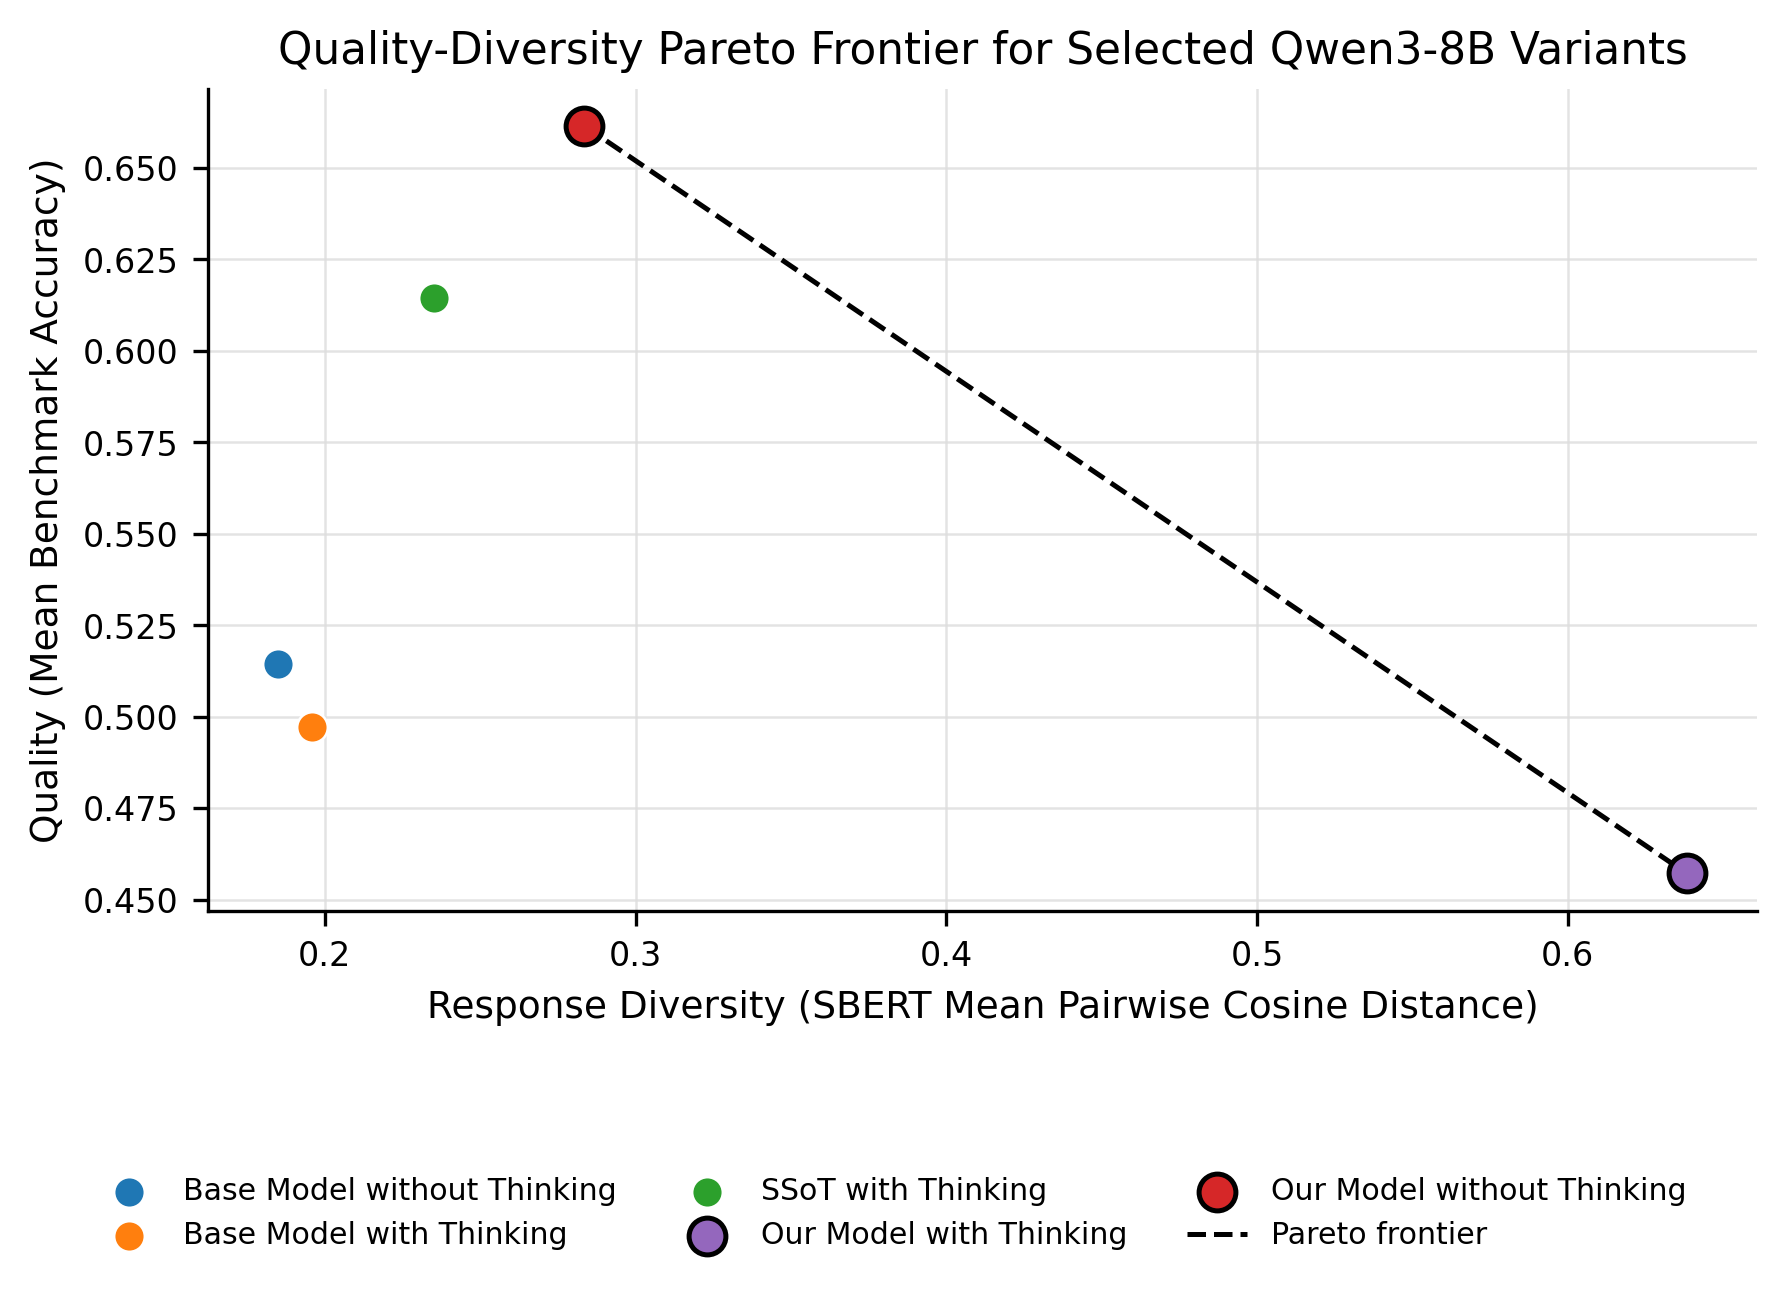
\includegraphics[width=\textwidth]{figures/pareto}
% \vspace{-0.5cm}
% \label{fig:intro}
% \end{figure}

\textbf{Generative Diversity Evaluation.} As shown in Figure~\ref{fig: domain application pareto}a, \method{} Pareto-dominates all baselines on the held-out Infinite-Chat set across every setting (thinking enabled/disabled, different base models), achieving both higher diversity and higher quality simultaneously; the remaining settings are shown in Appendix~\ref{appx:generative diversity evaluation}. We provide a breakdown by individual benchmarks in Table~\ref{tab:domain-app-diversity-main}. Across four domains and three model families, \method{} achieves the best average diversity across all evaluated baselines, while matching or improving quality on most domains except PreScience. Notably, \method{} outperforms all baselines on HypoBench, a scientific ideation task that is out of domain relative to our training set, which primarily consists of standard SFT data and open-ended questions. These results suggest that \method{} enhances general exploration capability across thinking settings and base models, even on out-of-domain topics.

\begin{figure}[ht]
\centering
\begin{minipage}{0.45\linewidth}
  \centering
  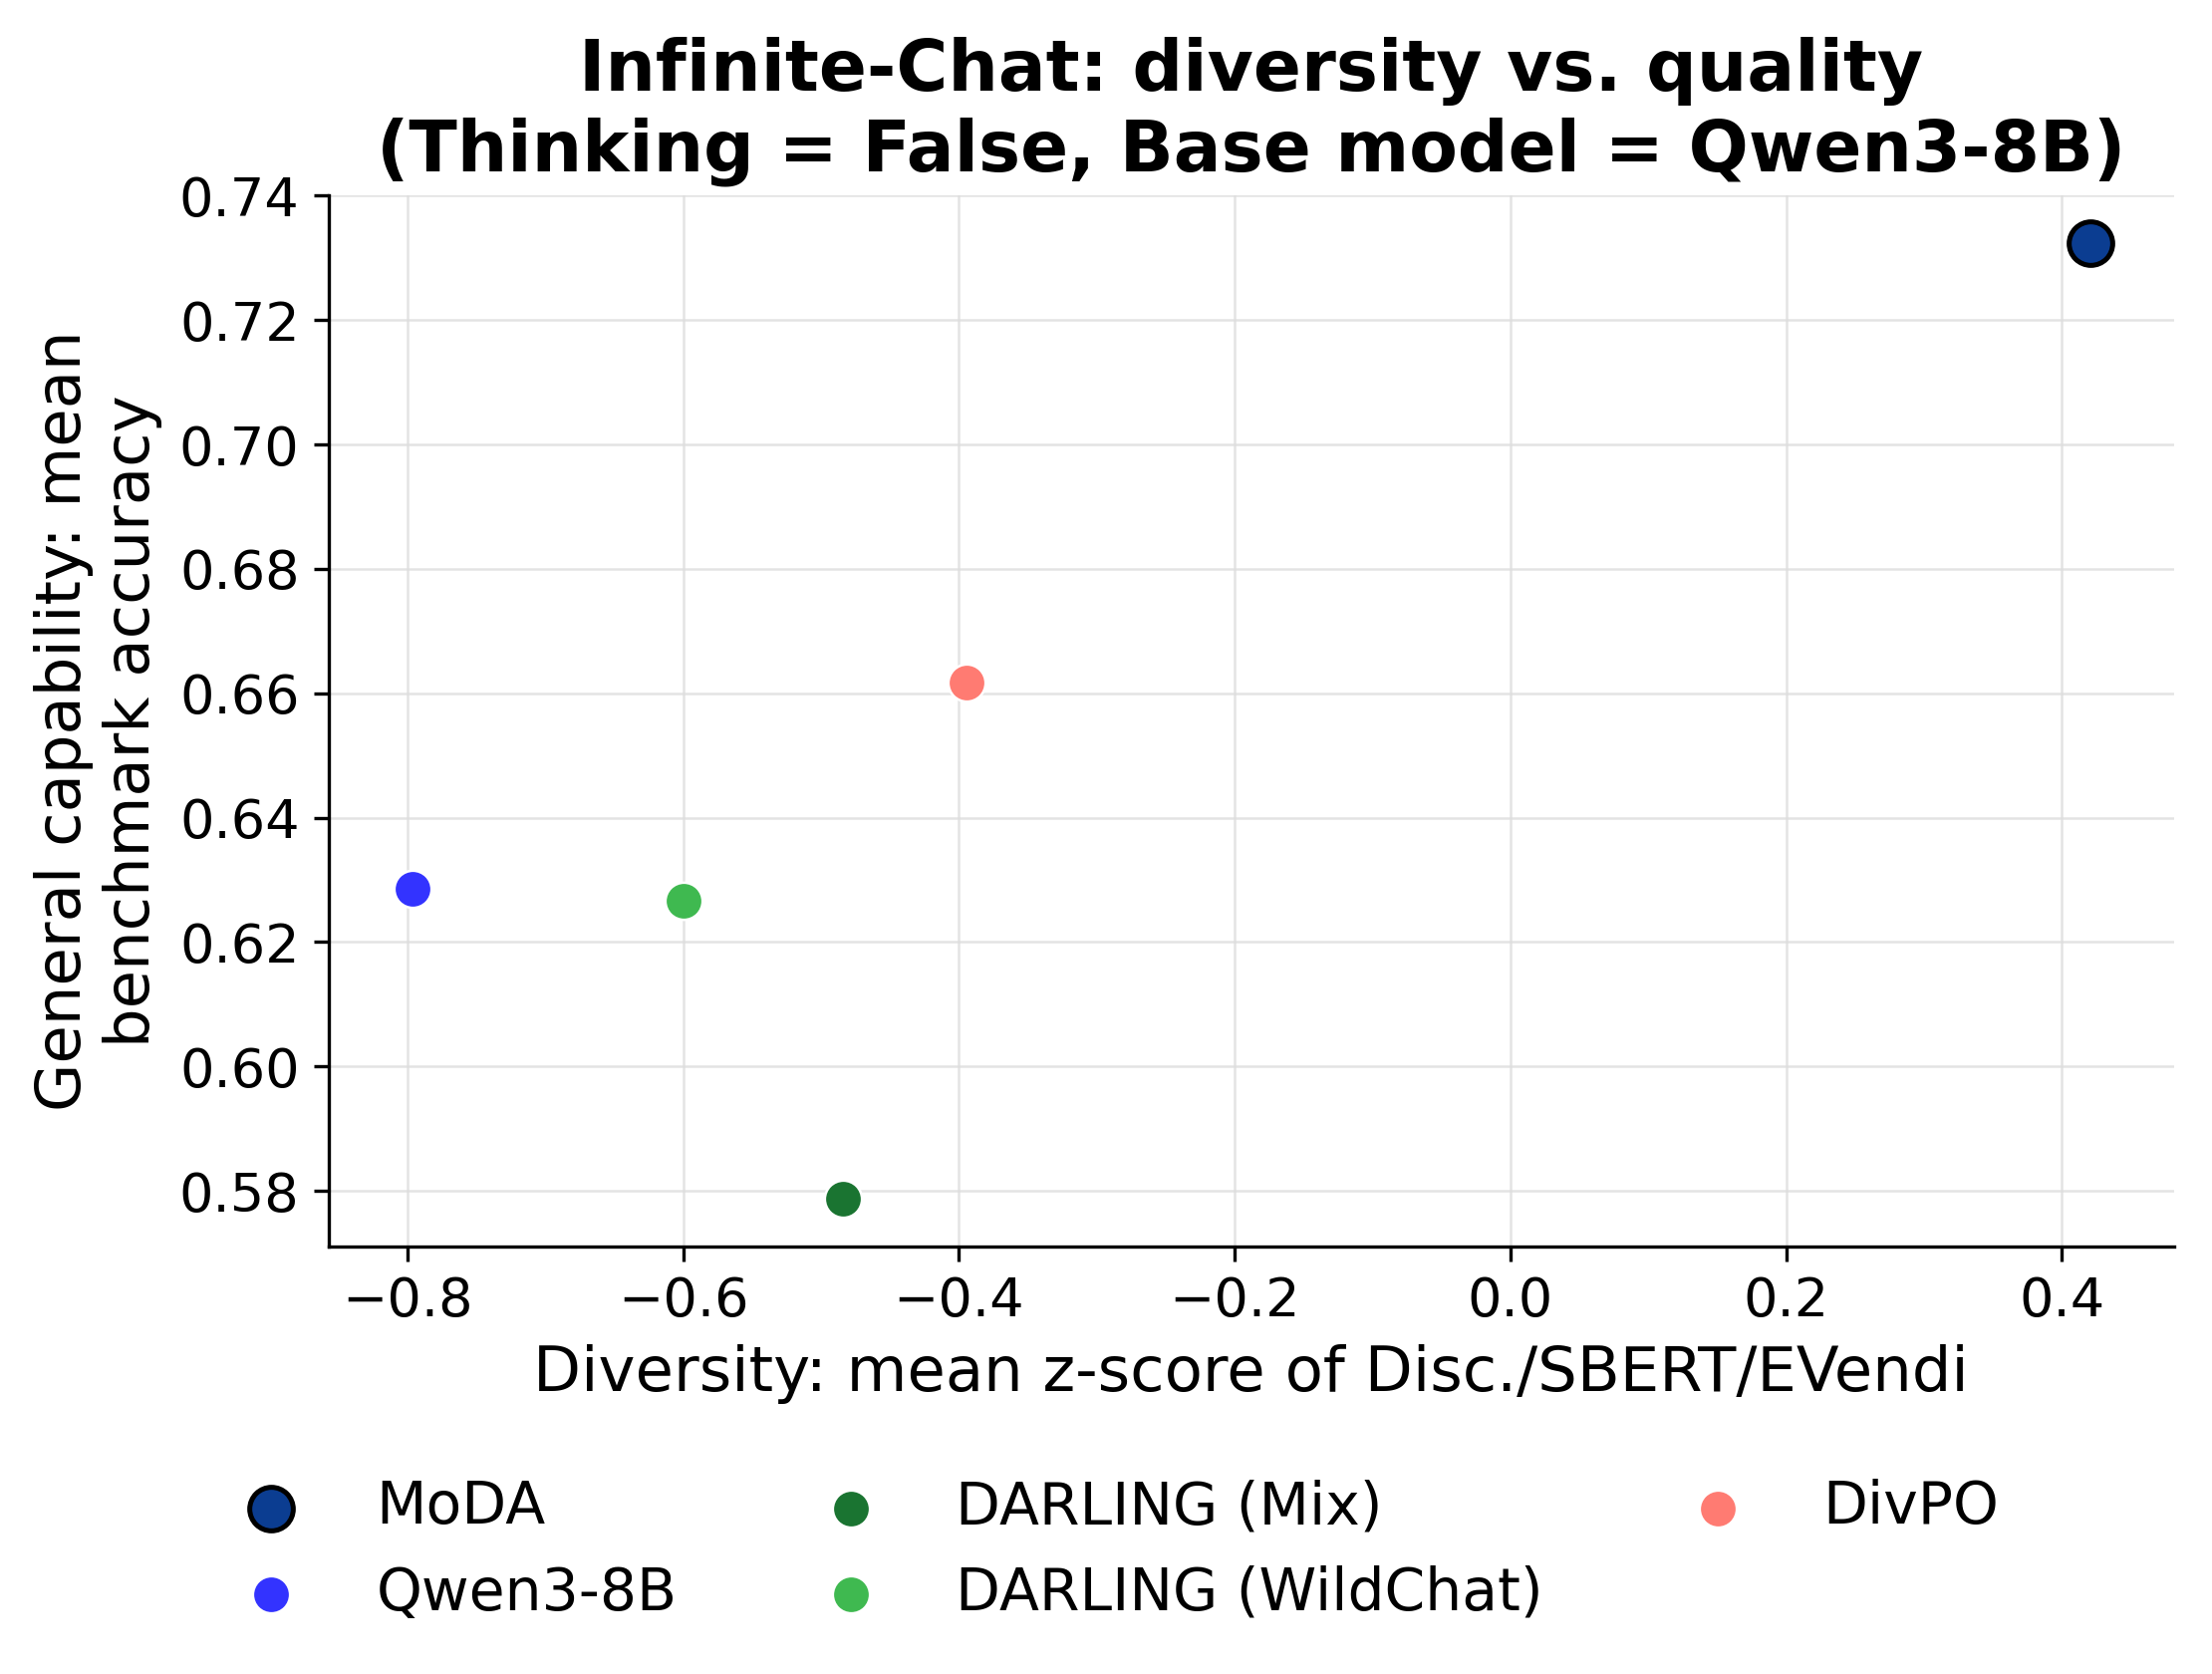
\includegraphics[width=\linewidth]{figures/pareto_infinite-chat_quality_thinking_false_base_model_qwen3-8b_composite.png}
  \small (a) Baselines
  \label{fig: domain application pareto baselines}
\end{minipage}\hfill
\begin{minipage}{0.5\linewidth}
  \centering
  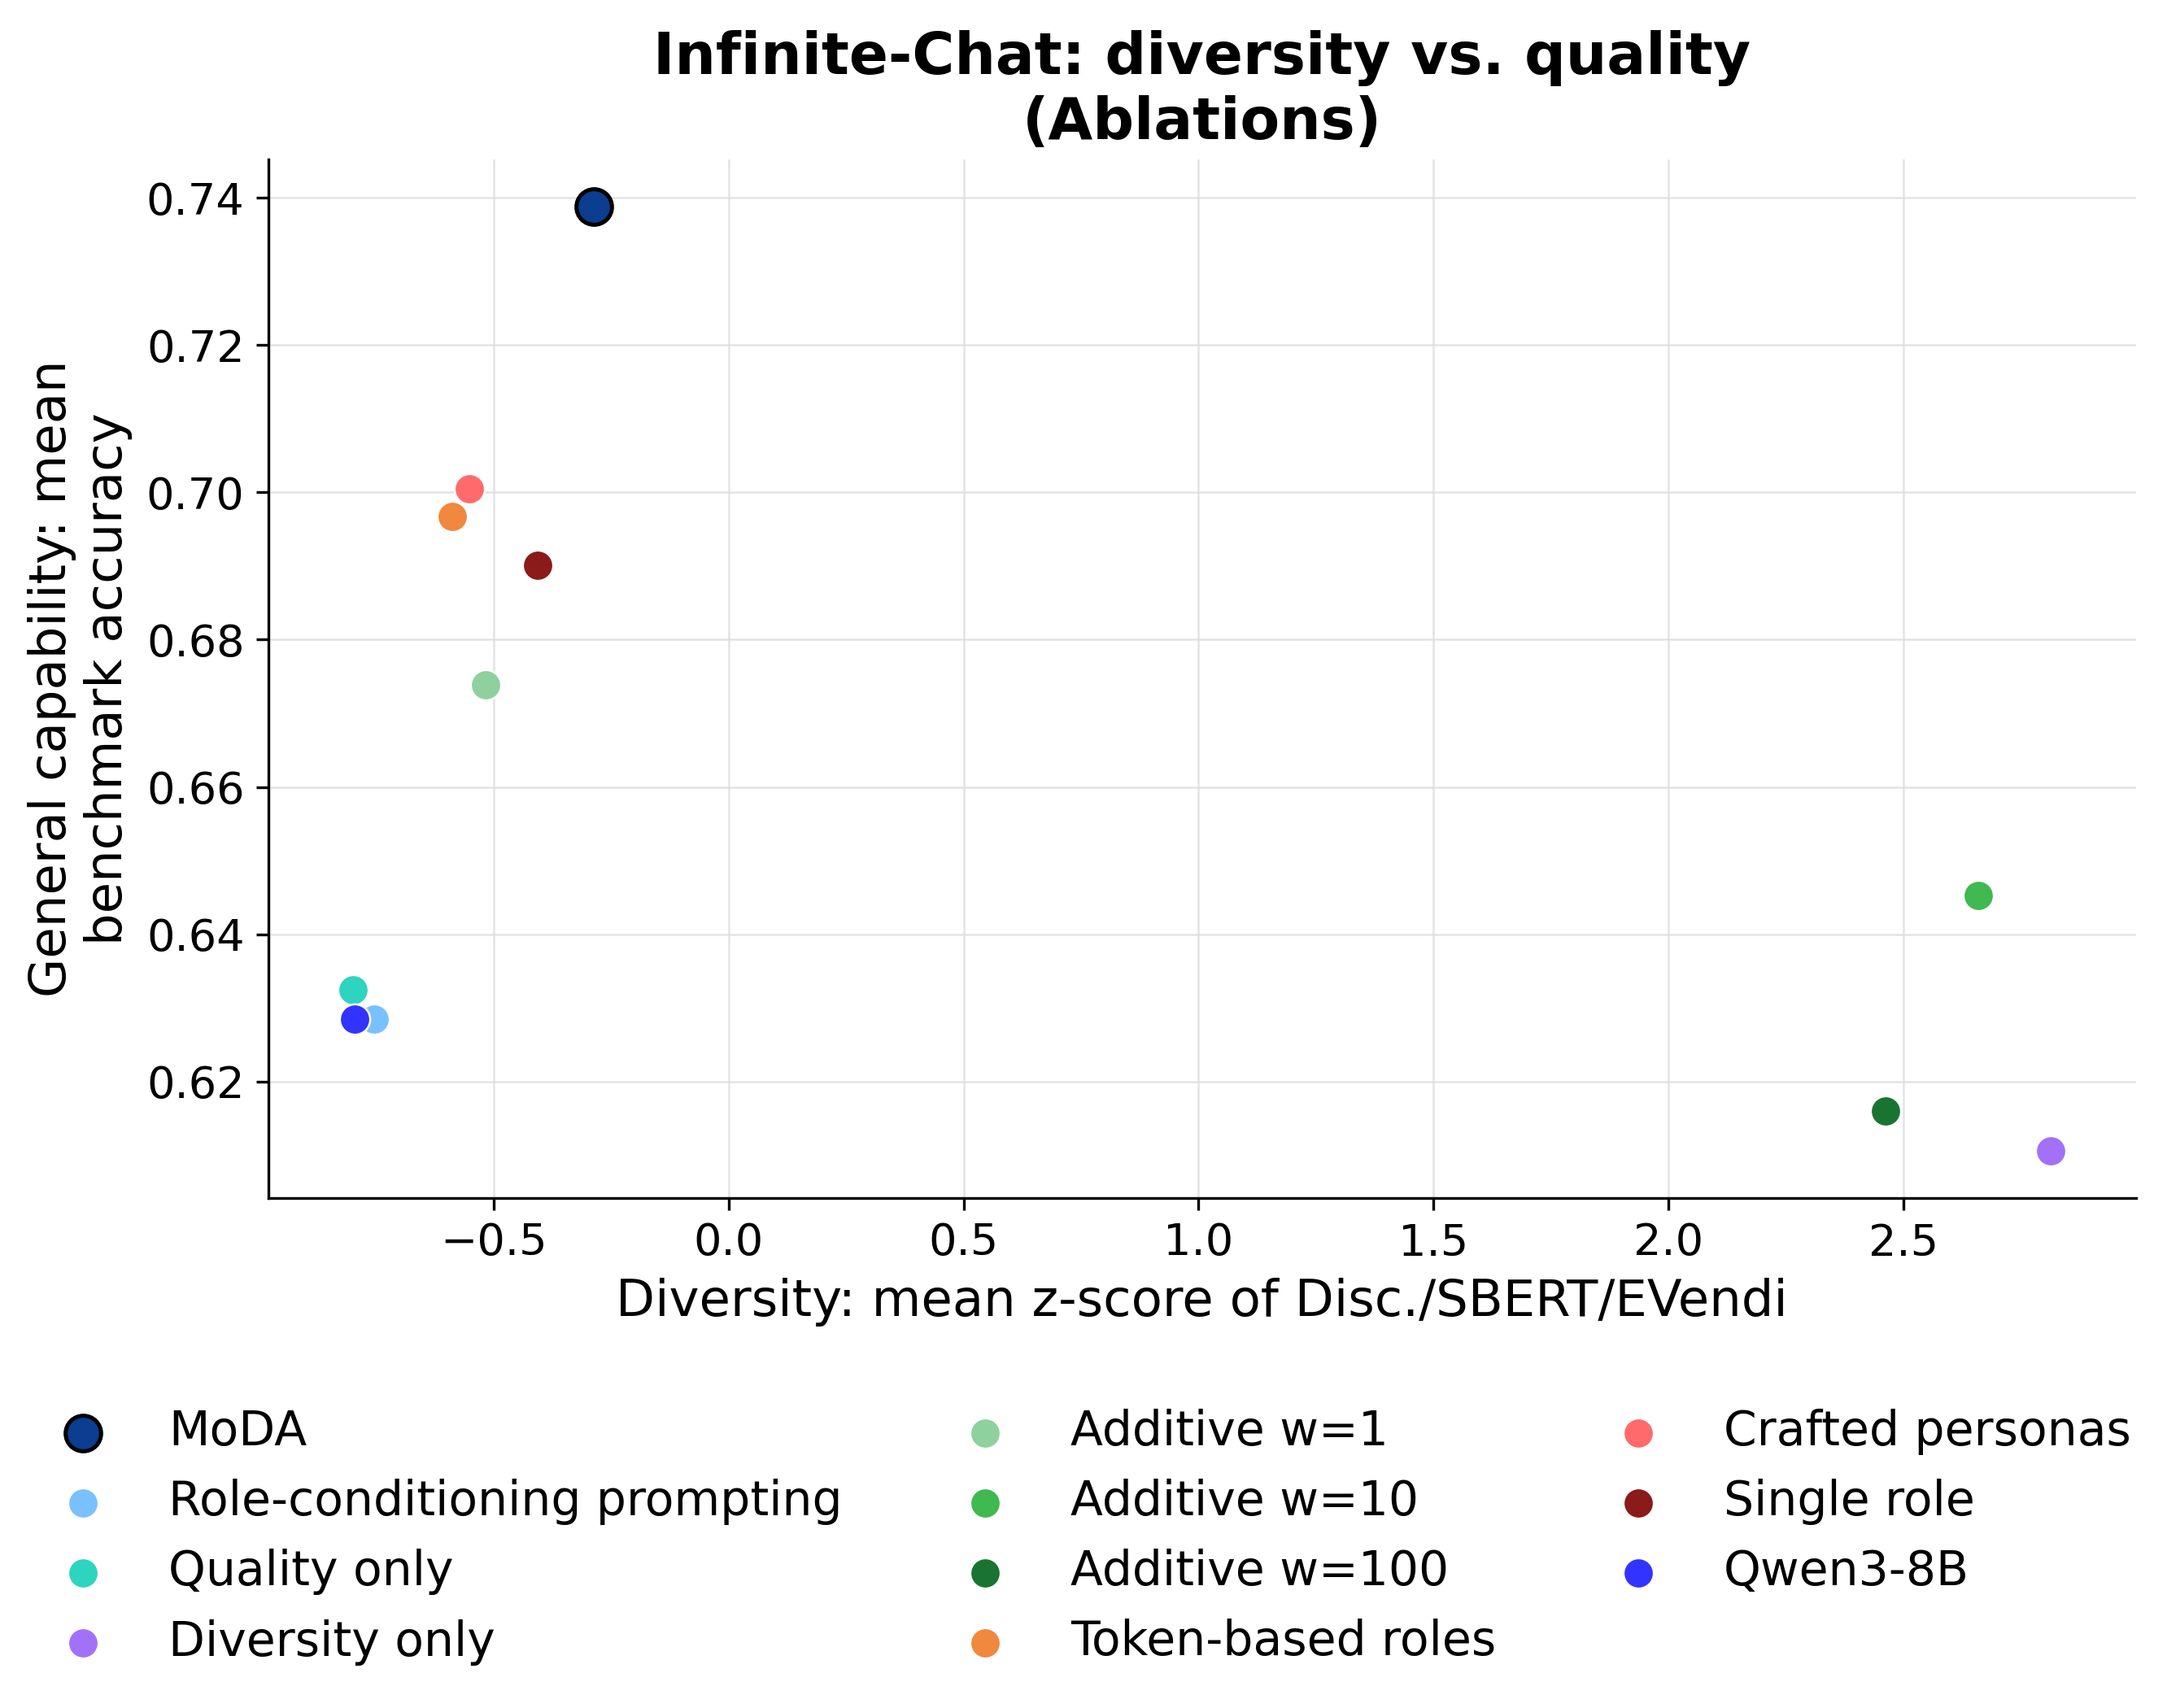
\includegraphics[width=\linewidth]{figures/pareto_infinite-chat_quality_ablations_composite.png}
  \small (b) Ablation variants
  \label{fig: domain application pareto ablations}
\end{minipage}
\caption{\textbf{Quality-diversity pareto front (Qwen3-8B, thinking disabled) baselines and ablated variants.} The x-axis is Infinite-Chat response diversity (mean z-score of Disc./SBERT/EmbVendi) and the y-axis is general capability (mean benchmark accuracy). \textbf{(a)} \method{} Pareto-dominates all the baselines, achieving better diversity and quality simultaneously. Results for Qwen3-8B (thinking enabled) and Llama-3.1-8B / GLM-4-9B (thinking disabled) are shown in Appendix~\ref{appx:generative diversity evaluation}. \textbf{(b)} The same comparison across \method{}'s ablated variants.}
\label{fig: domain application pareto}
\end{figure}

\begin{table*}[t]
\centering
\setlength{\tabcolsep}{3pt}
\resizebox{\textwidth}{!}{%
\begin{tabular}{lccccccccccccccccccc}
\toprule
Model & \multicolumn{4}{c}{\textit{Infinite-Chat}} & \multicolumn{4}{c}{\textit{NoveltyBench}} & \multicolumn{4}{c}{\textit{HypoBench}} & \multicolumn{4}{c}{\textit{PreScience}} & \multicolumn{3}{c}{Avg.} \\
\cmidrule(lr){2-5} \cmidrule(lr){6-9} \cmidrule(lr){10-13} \cmidrule(lr){14-17} \cmidrule(lr){18-20}
 & Disc. & SBERT & E-V & Qual.(\%) & Disc. & SBERT & E-V & Qual & Disc. & SBERT & E-V & Qual. & Disc. & SBERT & E-V & Qual. & Disc. & SBERT & E-V \\

\midrule
\multicolumn{9}{l}{\textsc{\underline{Qwen3-8B base, thinking disabled}}} \\
Qwen3-8B & 0.400 & 0.132 & 1.83 & 62.9  & 0.493 & 0.224 & 2.36 & 4.58 & 0.384 & 0.144 & 1.91 & \textbf{4.03} & 0.431 & 0.155 & 1.94 & \textbf{4.25} & 0.427 & 0.164 & 2.01 \\
DARLING (Mix) & \underline{0.430} & 0.203 & 2.33 & 57.9  & 0.513 & 0.281 & 2.96 & \underline{5.24} & 0.406 & \underline{0.222} & \underline{2.48} & 3.44 & \textbf{0.559} & \textbf{0.541} & \textbf{4.73} & 2.33 & \underline{0.477} & \underline{0.312} & \underline{3.12} \\
DARLING (WildChat) & 0.416 & 0.185 & 2.15 & 62.7  & 0.480 & 0.335 & 3.11 & 4.00 & 0.415 & 0.205 & 2.34 & 3.73 & 0.446 & 0.192 & 2.21 & \underline{4.03} & 0.439 & 0.229 & 2.45 \\
DivPO & 0.410 & \underline{0.274} & \underline{2.86} & \underline{66.2}  & \underline{0.519} & \underline{0.380} & \underline{3.58} & 4.87 & \underline{0.427} & 0.198 & 2.30 & \underline{3.89} & \underline{0.455} & \underline{0.233} & \underline{2.41} & 3.96 & 0.453 & 0.271 & 2.79 \\
\method & \textbf{0.472} & \textbf{0.482} & \textbf{4.40} & \textbf{73.2}  & \textbf{0.537} & \textbf{0.470} & \textbf{4.19} & \textbf{5.47} & \textbf{0.480} & \textbf{0.547} & \textbf{4.91} & 3.80 & 0.440 & 0.176 & 2.10 & 3.96 & \textbf{0.482} & \textbf{0.419} & \textbf{3.90} \\
\midrule
\multicolumn{9}{l}{\textsc{\underline{Qwen3-8B base, thinking enabled}}} \\
Qwen3-8B & 0.400 & 0.136 & 1.85 & 75.8  & 0.510 & 0.258 & 2.67 & \underline{4.90} & 0.399 & 0.164 & 2.05 & \textbf{3.93} & 0.441 & 0.136 & 1.83 & \underline{3.79} & 0.438 & 0.174 & 2.10 \\
SSoT & 0.397 & 0.178 & 2.09 & \underline{76.3}  & 0.438 & 0.239 & 2.57 & 0.46 & \underline{0.419} & \underline{0.220} & \underline{2.33} & 3.75 & \textbf{0.461} & \textbf{0.281} & \textbf{2.39} & 3.30 & 0.429 & \underline{0.230} & 2.34 \\
DivPO & \underline{0.414} & \underline{0.200} & \underline{2.20} & 71.7  & \underline{0.521} & \underline{0.327} & \underline{3.12} & \textbf{5.06} & 0.409 & 0.162 & 2.04 & \underline{3.89} & \underline{0.448} & 0.185 & 2.04 & \textbf{3.87} & \underline{0.448} & 0.218 & \underline{2.35} \\
\method & \textbf{0.600} & \textbf{0.909} & \textbf{9.04} & \textbf{76.8}  & \textbf{0.589} & \textbf{0.800} & \textbf{7.63} & 3.39 & \textbf{0.579} & \textbf{0.875} & \textbf{8.06} & 3.71 & 0.439 & \underline{0.194} & \underline{2.10} & 3.68 & \textbf{0.552} & \textbf{0.695} & \textbf{6.71} \\

\multicolumn{20}{l}{\textsc{\underline{{Llama-3.1-8B base, thinking disabled}}}} \\
Llama-3.1-8B & 0.414 & 0.217 & 2.40 & 46.7  & 0.512 & 0.312 & 3.04 & 4.80 & \textbf{0.469} & 0.207 & 2.38 & 3.60 & 0.461 & \textbf{0.514} & 3.67 & \textbf{2.62} & \textbf{0.464} & 0.312 & 2.87 \\
\method{} (Llama-3.1-8B) & \textbf{0.441} & \textbf{0.373} & \textbf{3.77} & \textbf{51.9}  & \textbf{0.532} & \textbf{0.392} & \textbf{3.75} & \textbf{6.17} & 0.410 & \textbf{0.324} & \textbf{3.27} & \textbf{3.65} & \textbf{0.472} & 0.470 & \textbf{3.89} & 2.54 & \textbf{0.464} & \textbf{0.390} & \textbf{3.67} \\
\midrule
\multicolumn{20}{l}{\textsc{\underline{GLM-4-9B base, thinking disabled}}} \\
GLM-4-9B & 0.421 & 0.234 & 2.60 & 44.9  & \textbf{0.544} & 0.408 & 4.08 & \textbf{4.14} & 0.402 & 0.225 & 2.52 & \textbf{3.75} & 0.461 & 0.438 & 4.15 & 2.57 & 0.457 & 0.326 & 3.34 \\
\method{}(GLM-4-9b) & \textbf{0.481} & \textbf{0.528} & \textbf{5.14} & \textbf{60.7}  & 0.502 & \textbf{0.521} & \textbf{5.01} & 2.70 & \textbf{0.452} & \textbf{0.485} & \textbf{4.64} & 3.68 & \textbf{0.464} & \textbf{0.448} & \textbf{4.28} & \textbf{2.58} & \textbf{0.475} & \textbf{0.495} & \textbf{4.77} \\
\bottomrule
\end{tabular}
}
\caption{Per-domain diversity (Disc. = discriminator diversity, SBERT = SBERT embedding pairwise distance, E-V = E-Vendi score) and quality (Qual.), averaged over $n{=}3$ random seeds. Infinite-Chat quality is general capability accuracy (\%); all other domains use the native quality score. Bold marks the best value within each model group. Table with error bar can be found in Appx \ref{appx:generative diversity evaluation}.}
\label{tab:domain-app-diversity-main}
\end{table*}




\textbf{General Capability Retention.} As shown in Figure \ref{fig:general capability retention}, our model achieves the best overall average pass@1, pass@5 and pass@10 score for general capability retention across thinking settings and base models among all baselines. With Qwen3-8B base and thinking disabled, it matches or exceeds the base model on 5 out of 7 benchmarks and achieves the best score among all baselines on 4 of them on pass@1 accuracy. Notably, with the GLM-4-9B base, \method improves average pass@1 by 15.8 percentage points, including a 3.89x relative improvement on GSM8K and a 2.37x relative improvement on MMLU. These results suggest that our method is an effective alignment approach that preserves, and in several cases significantly improves, the model's capabilities. We note that the language mixing penalty is important to maintain quality in some cases; without it, quality drops due to reward hacking from language mixing.


%We attribute this to the language-mixing penalty applied during training, which addresses the base model's native language-mixing issue. These results suggest that our method is an effective alignment approach that preserves, and in several cases significantly improves, the model's general capabilities.

\begin{figure}[ht]
\centering
\begin{minipage}[ht]{0.6\linewidth}
  \centering
  \resizebox{\linewidth}{!}{%
  \begin{table}[H]
\small
\setlength{\tabcolsep}{2.5pt}
\centering
\begin{tabular}{l*{7}{>{\centering\arraybackslash}p{0.95cm}}|>{\centering\arraybackslash}p{0.95cm}}
\toprule
Model & GSM8K & MMLU & GPQA & BoolQ & HS & TQA & IFEval & Avg. \\
\midrule
\multicolumn{9}{l}{\textsc{\underline{Qwen3-8B base, thinking disabled}}} \\
Qwen3-8B & \underline{84.5} & \textbf{82.0} & \underline{41.4} & 83.1 & 48.4 & 22.2 & \textbf{78.4} & 62.9 \\
DARLING (Mixture) & 63.5 & 63.0 & 34.3 & 76.7 & 62.2 & \underline{52.4} & 53.0 & 57.9 \\
DARLING (WildChat) & 77.9 & 55.0 & 34.3 & \textbf{86.4} & \underline{68.8} & 43.2 & 73.0 & 62.7 \\
DivPO & 80.5 & \underline{81.0} & 40.4 & 83.5 & 62.8 & 37.7 & \underline{77.3} & \underline{66.2} \\
\method & \textbf{86.7} & \underline{81.0} & \textbf{52.0} & \underline{84.8} & \textbf{73.4} & \textbf{57.9} & 76.9 & \textbf{73.2} \\
\midrule
\multicolumn{9}{l}{\textsc{\underline{Qwen3-8B base, thinking enabled}}} \\
Qwen3-8B & \textbf{90.3} & \textbf{94.0} & 43.4 & \textbf{87.2} & 70.9 & 64.9 & \textbf{79.7} & 75.8 \\
SSoT & 84.3 & \underline{93.0} & \textbf{55.1} & \textbf{87.2} & \textbf{80.1} & \textbf{72.8} & 61.9 & \underline{76.3} \\
DivPO & \underline{84.9} & 91.0 & 44.4 & \underline{83.2} & 65.0 & 55.3 & 77.6 & 71.7 \\
\method & 83.9 & \underline{93.0} & \underline{50.5} & \textbf{87.2} & \underline{76.2} & \underline{67.2} & \underline{79.5} & \textbf{76.8} \\
\midrule
\multicolumn{9}{l}{\textsc{\underline{Llama-3.1-8B base, thinking disabled}}} \\
Llama-3.1-8B & 71.3 & 16.0 & 6.1 & \textbf{81.6} & 30.2 & 53.4 & 68.8 & 46.7 \\
\method(Llama-3.1-8B) & \textbf{74.9} & \textbf{30.0} & \textbf{18.7} & 75.6 & \textbf{38.5} & \textbf{54.7} & \textbf{70.8} & \textbf{51.9}\\
\midrule
\multicolumn{9}{l}{\textsc{\underline{GLM-4-9B base, thinking disabled}}} \\
GLM-4-9B & 21.8 & 35.0 & 19.7 & 74.5 & \textbf{68.0} & \textbf{44.8} & 50.3 & 44.9  \\
\method(GLM-4-9B) & \textbf{84.9} & \textbf{83.0} & \textbf{33.3} & \textbf{81.2} & 52.3 & 34.5 & \textbf{55.5} & \textbf{60.7} \\
\bottomrule
\end{tabular}
\vspace{4pt}
\caption{General capability retention (Pass@1 accuracy \%), averaged over $n=3$ random seeds. Bold marks the best value within each model group; underline marks the second-best value within the Qwen3-8B groups. Table with error bar can be found in Appendix \ref{appx:general capability retention} Table \ref{tab:general-capability-pass1-error-bar}.}
\label{tab:general-capability-pass1}
\end{table}%
  }
\end{minipage}\hfill
\begin{minipage}[ht]{0.38\linewidth}
  \centering
  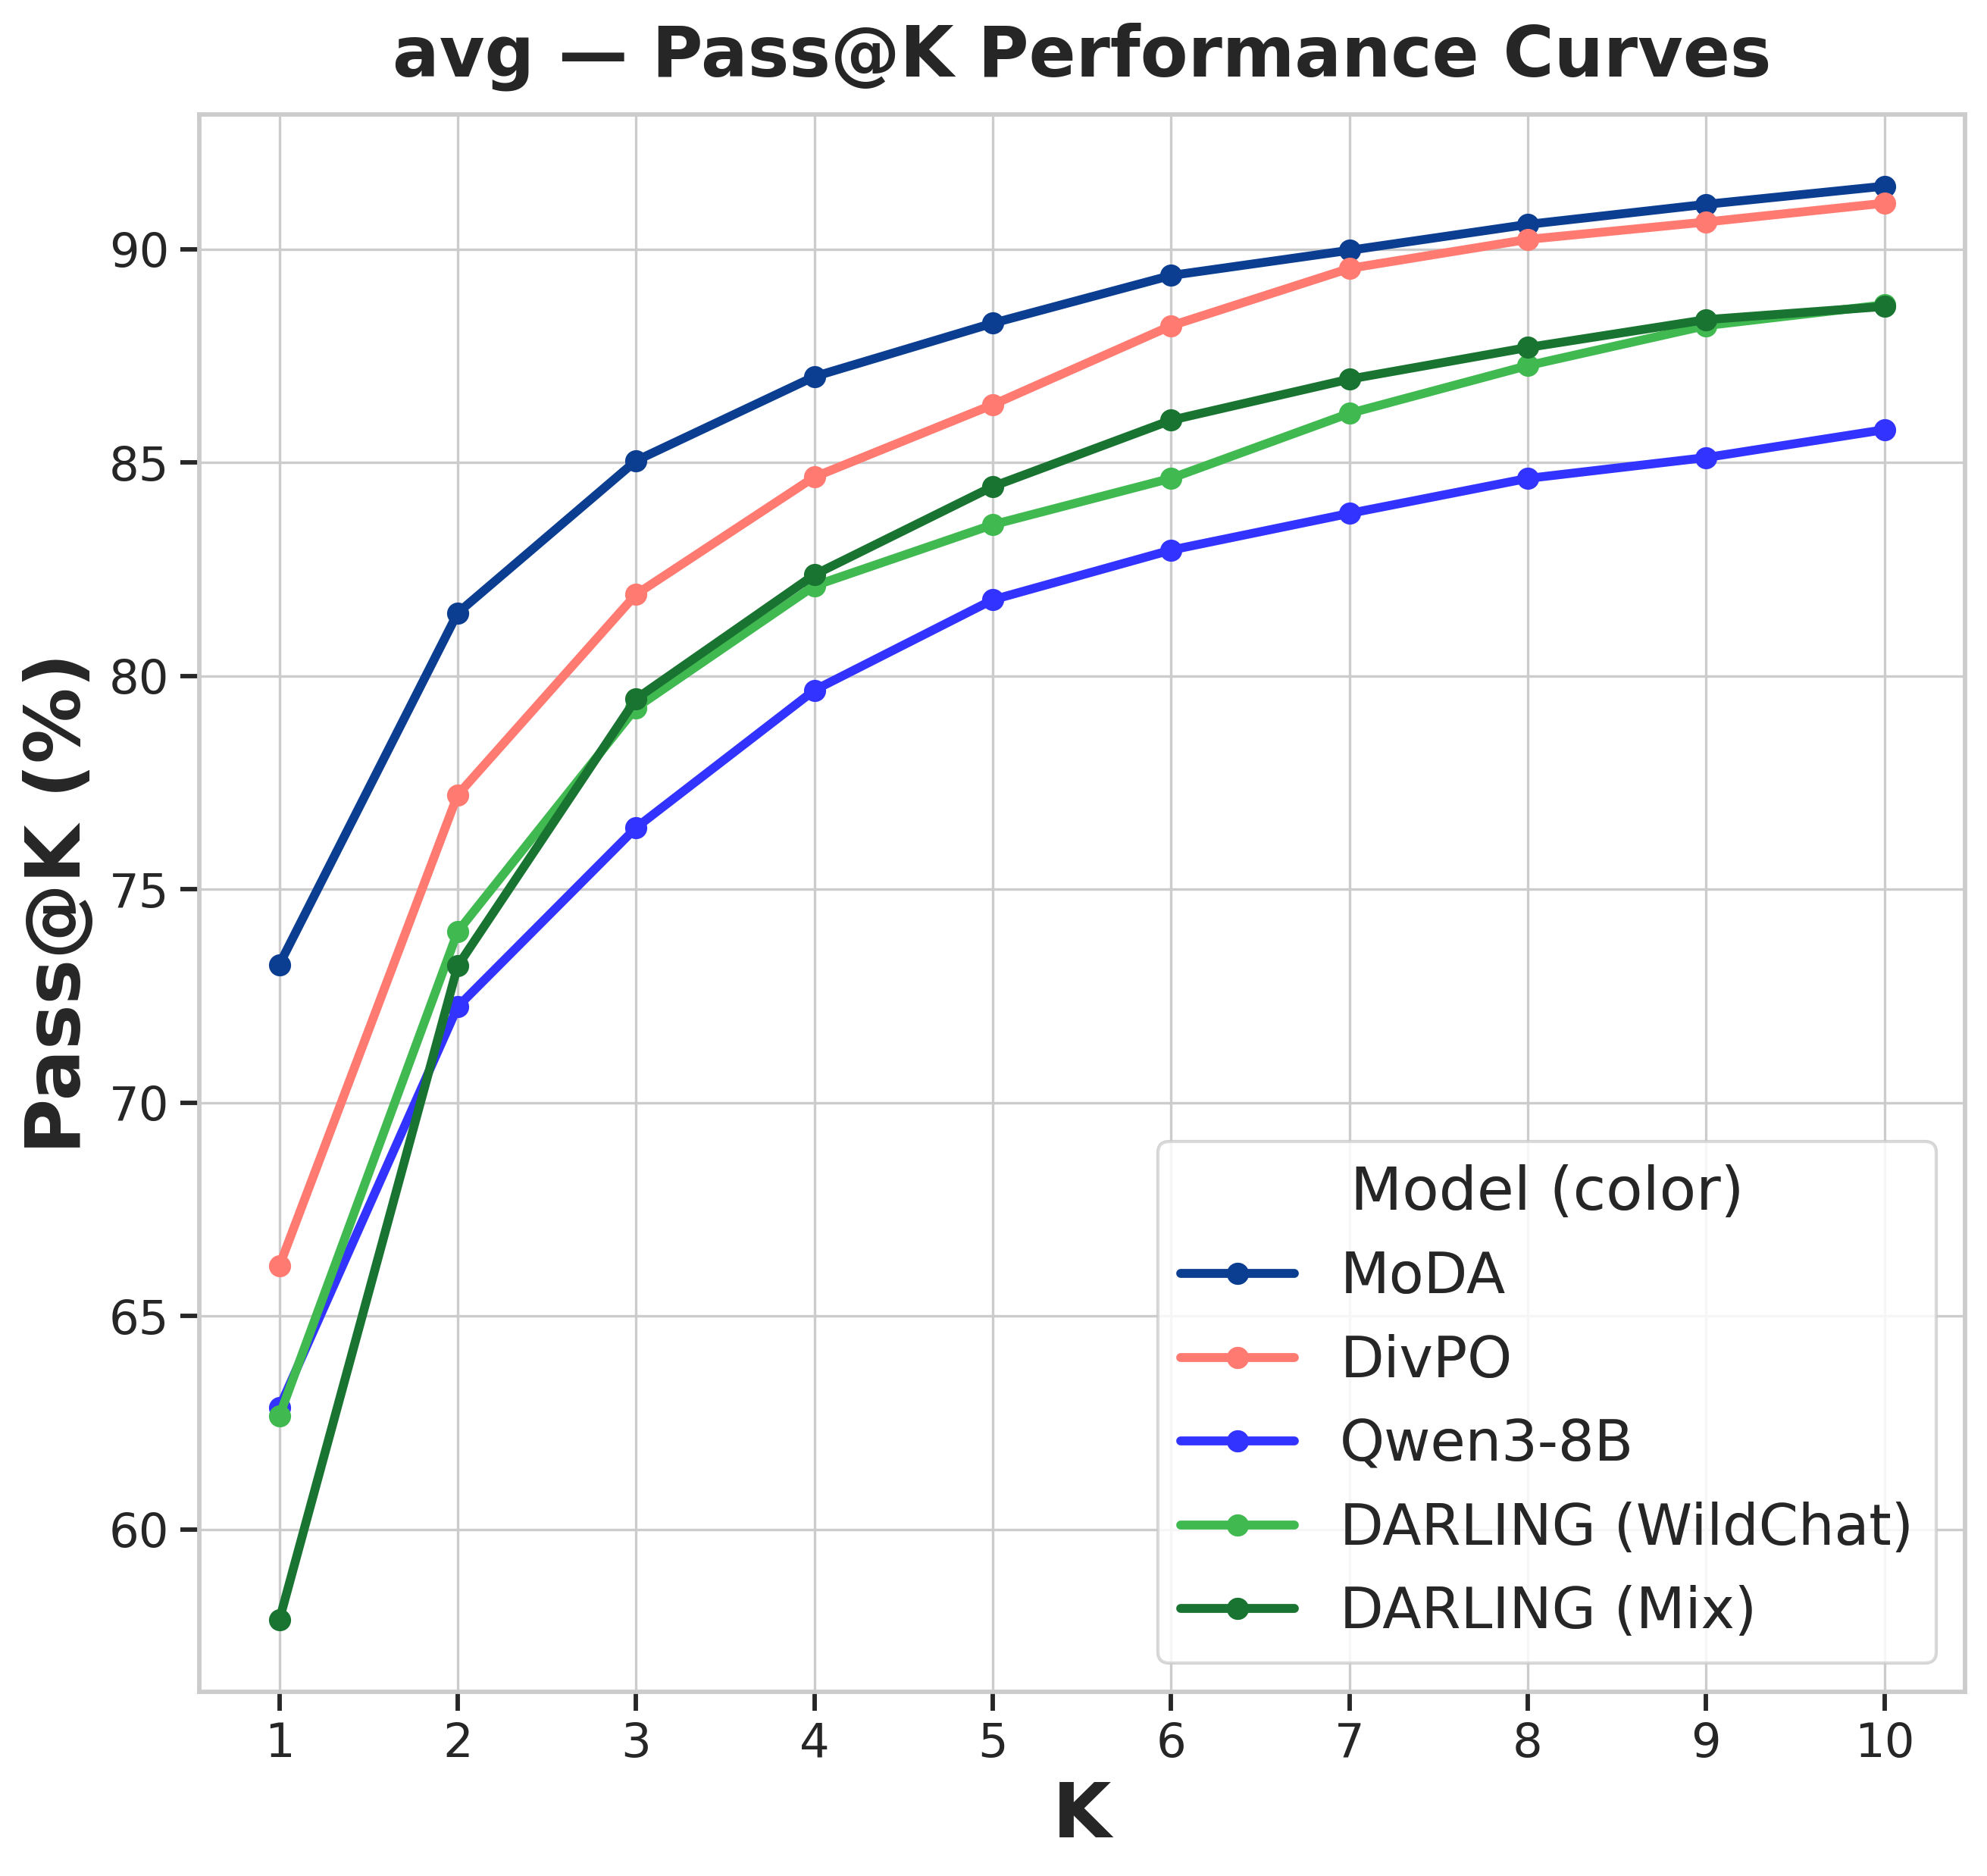
\includegraphics[width=\linewidth]{figures/main_pass_k/pass_at_k_figures/pass_at_k_avg_thinking_false_base_model_qwen3-8b.png}
\end{minipage}
\caption{\textbf{Left: General capability retention (Pass@1 accuracy \%)}, averaged over $n=3$ random seeds. Bold marks the best value within each model group; underline marks the second-best value within the Qwen3-8B groups. Table with error bar can be found in Appendix \ref{appx:general capability retention} Table \ref{tab:general-capability-pass1-error-bar}. \textbf{Right: General capability retention: pass@k accuracy.} Qwen3-8B base, thinking disabled models on the general capability suite average. Per-benchmark results are shown in Appendix \ref{appx:general capability retention} Figure \ref{fig:general capability pass@k thinking disabled}.}
\label{fig:general capability retention}
\end{figure}


% \begin{table}[H]
% \centering
% \small
% \setlength{\tabcolsep}{4pt}
% \begin{tabular}{lrrrr}
% \toprule
% Model Variant & HypoBench $\uparrow$ & PreScience $\uparrow$ & NoveltyBench $\uparrow$ & Infinite-Chat $\uparrow$ \\
% \midrule
% Base (No Thinking) & \textbf{4.025 $\pm$ 0.124} & \textbf{4.150 $\pm$ 0.191} & 4.403 & 0.514 $\pm$ 0.019 \\
% Ours (No Thinking) & 3.816 $\pm$ 0.075 & 3.602 $\pm$ 0.230 & \textbf{5.826} & \textbf{0.661 $\pm$ 0.018} \\
% \midrule
% Base (Thinking) & 3.920 $\pm$ 0.159 & 1.928 $\pm$ 0.206 & 3.147 & 0.497 $\pm$ 0.019 \\
% \ssot (Thinking) & 3.825 $\pm$ 0.113 & 1.494 $\pm$ 0.147 & 2.743 & 0.614 $\pm$ 0.018 \\
% Ours (Thinking) & 3.904 $\pm$ 0.114 & 3.581 $\pm$ 0.278 & 4.082 & 0.457 $\pm$ 0.019 \\

% \bottomrule
% \end{tabular}
% \caption{Aggregate domain-application quality across HypoBench, PreScience, NoveltyBench, and Infinite-Chat. Values are means with standard errors where available; NoveltyBench reports a single official aggregate in this run. Higher is better, and bold indicates the best model in each column.}
% \label{tab:domain-app-quality-error-bars}
% \end{table}

\subsection{Qualitative Results}
\label{sec:qualitative results}
We observe several interesting patterns in our experiments. Figure~\ref{fig:moda + 40blue} visualizes responses to the prompt \textbf{``Name a shade of blue''} from Qwen3-8B, Qwen3-8B with \ssot, and \method{} with thinking disabled. Consistent with the quantitative results, \method{} produces a larger set of valid and distinct responses. Interestingly, although \method{} uses only abstract numbered roles rather than hand-crafted personas, the model sometimes learns role-specific behavioral patterns, suggesting that abstract mode conditioning can induce differentiated characteristics, learned via competitive multi-agent training, without manually specifying each role. Figure~\ref{fig:qualitative-example-books-main} shows that, when asked to name a well-received book, the base model produces the same answer, ``To Kill a Mockingbird,'' in all six samples, whereas \method{} produces six distinct titles; additional qualitative examples are provided in Appendix~\ref{appx: generation examples}.
\liweiaddressed{can we pick example so that we can show across dirrent roles the generations are creative and different, while for other models, resampling doesn't give sufficiently creative candidates?}

\begin{figure}[ht]
\centering
\begin{promptbox}
\small\textit{Name one well received book that often appears in top book lists.}
\end{promptbox}
\begin{minipage}[t]{0.24\linewidth}
\begin{respbox}{Sample 1}
One well-received book that often appears in top book lists is \textbf{To Kill a Mockingbird} by Harper Lee. It is a classic of American literature and has consistently ranked high in various lists.
\end{respbox}
\end{minipage}\hfill%
\begin{minipage}[t]{0.24\linewidth}
\begin{respbox}{Sample 2}
One well-received book that often appears in top book lists is \textbf{To Kill a Mockingbird} by Harper Lee. It is widely celebrated for its powerful themes of racial injustice, morality, and empathy.
\end{respbox}
\end{minipage}\hfill%
\begin{minipage}[t]{0.24\linewidth}
\begin{modarespbox}{Role 1}
\textbf{``The Night Fire''} by Michael Connelly. \textbf{Award-winning author}: known for his intelligent, fast-paced crime fiction.
\end{modarespbox}
\end{minipage}\hfill%
\begin{minipage}[t]{0.24\linewidth}
\begin{modarespbox}{Role 2}
\textbf{``The Night Circus''} by Erin Morgenstern. Known for its richly imaginative world-building and lyrical prose.
\end{modarespbox}
\end{minipage}
\caption{\textbf{Qualitative example of diverse generation.} \textbf{Left two:} Qwen3-8B repeats the same title across samples. \textbf{Right two:} \method{} under distinct numbered roles produces conceptually distinct titles for the same prompt. More samples in Appendix~\ref{appx: generation examples} Figure~\ref{fig:qualitative-example-books}.}
\label{fig:qualitative-example-books-main}
\end{figure}


\subsection{Ablation Studies.}
% \begin{table}[H]
\centering
\setlength{\tabcolsep}{3pt}
\resizebox{\textwidth}{!}{%
\begin{tabular}{lccccc}
\toprule
& \multicolumn{2}{c}{General capability (Avg., \%)} & \multicolumn{3}{c}{Infinite-Chat Diversity} \\
\cmidrule(lr){2-3} \cmidrule(lr){4-6}
Ablation & Standard mode & Diverse mode & Disc. & SBERT & E-Vendi \\
\midrule
Role-conditioned prompting & 62.9  & 56.6  & 0.403  & 0.145  & 1.90  \\
Quality only & 63.2  & 61.8  & 0.401  & 0.131  & 1.82  \\
Diversity only & 61.1  & 10.7  & \textbf{0.656}  & \textbf{0.993}  & \textbf{9.77}  \\
Additive $w{=}1$ & 67.4  & 68.0  & 0.422  & 0.204  & 2.33  \\
Additive $w{=}10$ & 64.5  & 5.7  & 0.632  & 0.976  & 9.64  \\
Additive $w{=}100$ & 61.6  & 5.4  & 0.621  & 0.970  & 8.75  \\
Token-based roles & 69.7  & 67.9 & 0.419 & 0.197 & 2.04 \\
Crafted personas & 70.1  & 66.1  & 0.421  & 0.194  & 2.24  \\
Single role & 69.0  & 69.9  & 0.428  & 0.239  & 2.57  \\
\midrule
Qwen3-8B & 62.9 & - & 0.400 & 0.132 & 1.83 \\
\midrule
\textbf{\method{}} & \textbf{73.2}  & \textbf{71.6}  & 0.444  & 0.257  & 2.69  \\
\bottomrule
\end{tabular}
}
\vspace{4pt}
\caption{\textbf{Ablation results} for general capability (Pass@1) under standard and diverse decoding (accuracy \%) and Infinite-Chat diversity ($n{=}3$ random seeds). Bold marks the best value per column.}
\label{tab:ablation}
\vspace{-0.6cm}
\end{table}
% In this section, we perform ablation studies on the design choices of \method. 

\paragraph{Ablation Setups.}
First, to understand whether the diversity improvement comes from training or solely from role injection, we inject numbered roles to the base model (\textbf{Role-conditioned prompting}). Second, to examine whether the diversity gains are driven by the explicit diversity reward or arise naturally from repeated sampling and RL optimization, we trained \method{} with \textbf{Diversity only} reward and \textbf{Quality only} reward. Third, to understand the effect of quality-gated diversity reward, we trained \method{} with additive reward of weighted sum of quality and diversity metrics, with diversity weight = 1, 10 and 100 (\textbf{Additive w=1\textbackslash10\textbackslash 100}). Finally, to understand the effect of the naive numbered role injection, we trained several variants of \method: (1) \textbf{Crafted personas}, which conditions the roles with manually crafted persona descriptions (e.g. ``You are a creative problem solver.''; (2) \textbf{Single role}, conditions with only one role; (3) \textbf{Token-based roles}\liweiaddressed{again I think we should change this name to something a bit more serious.}, conditions the role with a dummy token (e.g. ``Start your response with APPLE.''). More implementation details are in Appendix \ref{appx: ablation model implementations}. We evaluate each ablated variants for general capability under standard and diverse decoding, and application domain suite under diverse decoding, with full results in Appendix \ref{appx: ablation results}.

\liweiaddressed{add a paragraph title to this, like the follwing two paragraphs.}
\textbf{Quality-Diversity Trade-off.} As shown in Figure~\ref{fig: domain application pareto}b, \method{} achieves the best accuracy on the general capability suite among all variants. \method{} also achieves 77\% higher SBERT diversity and 41.6\% higher E-Vendi diversity than role-conditioning prompting alone, indicating that role-conditioning prompting by itself is insufficient to induce diverse generation. The quality-only variant regresses in diversity relative to role-conditioning prompting, suggesting that an explicit diversity objective is necessary for diversity gains. The diversity-only variant achieves the best diversity metrics overall, but with the lowest accuracy under standard decoding, and its performance collapses entirely under diverse decoding, indicating that explicit quality gating is critical to preserving response quality.

\textbf{Additive Aggregation.}\label{ablation: additive aggregation} Many existing works on quality-diversity optimization aggregate quality and diversity objectives using a weighted sum~\citep{mouret2015illuminatingsearchspacesmapping, Chen2025PosttrainingLL}. We compare our method with variants trained using an additive reward objective. We find that additive aggregation is highly sensitive to the diversity weight $\lambda_d$. at $\lambda_d=1$, the additive variant shows modest diversity improvement over the baseline, but substantially less than \method{}; at $\lambda_d=10$ and $\lambda_d=100$, diversity improves significantly, but at the cost of general capability performance under diverse decoding. In contrast, \method{} separates quality control from diversity optimization through the quality gate, making the reward less sensitive to coefficient scaling and enables faster iteration.

\textbf{Role Injection.}
\label{ablation: role injection}
Prior work has shown that manually designed prompts can induce different model
behaviors \citep{park2024generative, argyle2023out}. We therefore craft six personas and inject them into the system prompt instead of the abstract numbered roles, testing whether hand-designed personas provide a stronger diversity prior than the abstract numbered role used in the main setting. To isolate the effect of role multiplicity from role content, we train a single-role variant in which every response is generated under the same \textit{``You are Role 1.''} system prompt. To study the effect of the identity-based role, we train a token-based conditioning variant in which the system prompt instructs a token-based distinguishing signal (e.g. \textit{``Start your response with APPLE/BANANA/ORANGE.''}).
As shown in Table~\ref{tab:ablation}, all variants exhibit a slight diversity improvement over the base model, but their gains are smaller than \method{}'s, indicating that multiple abstract numbered identity-based role provides a more effective exploration space than all the ablated variants, without sacrificing generalization.
\section{Discussions}
\label{sec:discussions}

In this work, we introduced \method, an online-MARL-inspired alignment method that encourages diverse generation while preserving response quality. \method~serves as a drop-in replacement for existing post-training alignment pipelines, requiring no architectural modifications to the underlying model. Compared to previous methods, its dual-mode design enables seamless switching between producing a single high-confidence answer and generating a diverse set of plausible responses, offering greater flexibility depending on the downstream needs. The ability to surface conceptually distinct yet high-quality responses has broad implications for high-stakes domains such as medical diagnosis, legal reasoning, and scientific ideation.

\textbf{Limitations and Future Work.} Several limitations point to promising directions for future research. First, our quality reward model (SkyReward-V2) tends to favor verbose responses, even for prompts that should be answered briefly, and our uniform length penalty insufficiently addresses this across prompts of varying complexity. For instance, when training GLM-4-9B with \method, we observed suboptimal native quality score on NoveltyBench compared to the base model because its reward model doesn't penalize verbosity therefore it reward hack by adding unnecessary preambles such as ``As a model.../To answer these questions as a model...'' Removing these preambles  recovers the performance from 2.739 to 3.302 (+20\%). Future work should explore adaptive length penalties or alternative reward models that better reflect conciseness. Second, because \method~introduces no external data during training, generative diversity is bounded by the initial policy's capacity, and incorporating retrieval augmentation or external data sources could meaningfully expand the exploration space. Finally, there is a risk of producing more varied but misleading, unsafe, or unsupported outputs, especially in high-stakes domains such as medical diagnosis and legal reasoning. Although \method~mitigates this through its dual-mode design, whose standard mode retains the model's general capability, future work can further combine the diverse mode with verification, calibration, retrieval, or domain-specific safeguards.
\section*{Acknowledgment}
We thank our colleagues at the SocialRL Lab at the University of Washington for their valuable feedback and support. The work of Natasha Jaques was supported by the UW-Amazon Science Gift Hub, UW-Tsukuba Amazon NVIDIA Cross Pacific AI Initiative (XPAI), Sony Research Award, Character.AI, DoorDash, Open Philanthropy, Toyota Research Institute, and the Schmidt AI2050 Fellows program. This work was supported by DARPA under the ITM program (FA8650-23-C-7316). The views expressed are those of the author and do not reflect the official policy or position of the Department of Defense or the U.S.~Government.

% This work was also supported in part by the Defense Advanced Research Projects Agency's (DARPA) SciFy program (Agreement No. HR00112520300). 


\newpage
% \input{checklist}
\bibliography{reference}
\bibliographystyle{plain}
\onecolumn
\newpage
\appendix

\begin{appendices}

\startcontents[sections]
\printcontents[sections]{l}{1}{\setcounter{tocdepth}{2}}

\clearpage
\newpage
\section{Discussions}
\label{asec:discussions}


\subsection{Limitations}
\label{assec:limitations}

While comprehensive with 26K queries, \dataset represents only a snapshot of the vast space of possible open-ended queries and may not capture all forms of creative divergence across different contexts. Moreover, the focus on English-language prompts derived from WildChat potentially underrepresents linguistic, cultural, and regional diversity in user interactions with language models, limiting the generalizability of our findings to non-English contexts and diverse cultural perspectives. To construct our taxonomy of queries, we used GPT-4o to efficiently label user queries, and we found human annotators achieved 74.7\% agreement with these automatic labels. While this accuracy could be improved, e.g., by labeling with stronger models or through model ensembling approaches, this performance is comparable to typical human annotation accuracy and we deem sufficient to represent the distribution of categories within our open-ended taxonomy.
Finally, while our analysis successfully reveals clear patterns such as the ``time is a river/weaver'' dichotomy, it may oversimplify the multidimensional nature of creative expression, and relying on semantic similarity of text embeddings to quantify diversity may lack sufficient expressiveness to capture the full spectrum of creative variation in generated responses.

While extending \dataset to multilingual and multicultural settings is an important direction, we anticipate that similar homogenization issues will likely arise across languages and cultures, given the global overlap in pretraining data sources and alignment practices. We encourage future work to pursue such extensions, and we hope our benchmark provides a comprehensive foundation that multilingual research can build upon. Our taxonomy was designed to be language-agnostic and can support adaptation when appropriate resources and expertise are available. We'll further strengthen this discussion in camera-ready.

Diversity and quality represent two key dimensions in evaluating responses to open-ended queries. In this work, we focused primarily on diversity, with fixed model decoding configurations, without studying quality. We selected a decoding configuration that generated empirically coherent text and investigated whether models can be guided to produce responses that maximize diversity while maintaining reasonable quality. Furthermore, we show that existing LMs, LM judges, and reward models struggle to reliably distinguish between equal-quality responses for open-ended queries. This motivates the need for further investigation into reliable automatic evaluation of equal-quality responses for open-ended queries, beyond human annotation. Finally, although our analysis identifies clear evidence of an ``Artificial Hivemind'' effect across models, it falls short of establishing the underlying mechanisms causing this homogenization. Future research can mechanistically disentangle causality, whether stemming from shared training data, memorization, generalization, or other factors.

Our work has significant implications for AI development and society, providing a valuable dataset for diagnosing and potentially mitigating LM homogenization and accelerating the development of more diverse, creative AI systems that align with diverse human needs and perspectives. However, this ``Artificial Hivemind'' effect also raises serious concerns about models' long-term impact on human creativity. If users increasingly rely on such systems for creative tasks, exposure to homogenized outputs could subtly influence human thinking patterns and reduce overall cultural and intellectual diversity. Furthermore, it could exacerbate existing biases and limit representation of marginalized perspectives. When LMs converge on dominant cultural expressions---such as Western-centric metaphors like ``time is a river"---they may inadvertently suppress alternative worldviews and traditions.

The ``Artificial Hivemind'' effect also highlights fundamental questions about what values we want AI systems to embody. Should AI prioritize efficiency and consistency, or diversity and novelty? These choices reflect deeper societal values about creativity, culture, and human flourishing. The ethical implications of LM homogenization extend far beyond technical considerations, touching on fundamental questions about human agency, cultural preservation, and the kind of future we want to create with these technologies. Addressing these challenges requires not just technical innovation, but sustained ethical reflection and inclusive dialogue about the role of AI in human creative expression.


\subsection{Future Directions}
\label{assec:future}

Our findings open several promising directions for advancing the study and mitigation of behavioral convergence in large language models.

\textbf{Foundation and training analysis.} We plan to extend the Artificial Hivemind testbed to foundation models without instruction-following capabilities to better disentangle the respective roles of pre-training and post-training in shaping convergent behaviors. Moreover, we aim to quantify the relative contributions of different post-training pipelines—such as supervised fine-tuning, RLHF/RLAIF, and constitutional training—to the emergence of homogenized responses.

\textbf{Mitigation and alignment strategies.} Future work will explore diversity-aware training objectives and alignment schemes that explicitly reward exploration of multiple valid modes while preserving response quality. We also intend to benchmark decoding strategies (e.g., diverse beam search, nucleus sampling variants) under the Artificial Hivemind metric to evaluate their effectiveness in counteracting homogenization.

\textbf{Practical integration.} To make our framework actionable, we will integrate Artificial Hivemind into red-teaming workflows to stress-test model robustness and coverage under open-ended queries. Additionally, our dataset can serve as a training prompt resource for reinforcement learning methods that explicitly encourage diversity during alignment. Finally, Hivemind’s diagnostic signals can inform curriculum design—gradually exposing models to increasingly open-ended prompts that are most susceptible to mode collapse.

Together, these directions position Artificial Hivemind as not only a descriptive diagnostic tool, but also a foundation for developing training, decoding, and evaluation practices that foster greater diversity and individuality in language models.

\subsection{Broader Implications}
\label{assec:broad}

\paragraph{Societal Implications.}
While some degree of convergence among large language models (LLMs) is statistically expected, its societal consequences warrant close scrutiny. As billions of users increasingly depend on LLMs for creative, educational, and decision-making purposes, understanding and quantifying behavioral homogenization becomes critical. Emerging evidence shows measurable shifts in human writing styles, creative ideation, and divergent thinking following the widespread adoption of systems like ChatGPT \cite{Kumar_2025,Anderson2024HomogenizationEO,Ashkinaze_2025,doi:10.1126/sciadv.adn5290,kosmyna2025brainchatgptaccumulationcognitive,sourati2025shrinkinglandscapelinguisticdiversity}. These findings suggest that model-level convergence may propagate into human expression, amplifying uniformity in linguistic and cognitive patterns at scale. By introducing quantitative tools to measure and track such convergence, our work provides an empirical foundation for assessing the long-term cultural and epistemic consequences of LLM-mediated communication.

\paragraph{Implications for Data Distillation and Model Training.}
Our results also have immediate implications for synthetic data generation and model training practices. While distilling knowledge from LLMs has proven transformative for efficiency and scalability, it is well known that relying on a single model as a teacher can intensify mode collapse, reinforcing narrow response patterns, diminishing output diversity, and, in extreme cases, leading to degenerative feedback loops \cite{alemohammad2024selfconsuming,kazdan2025collapsethriveperilspromises}. To counter this, recent approaches employ model swarms and multi-agent frameworks that aggregate outputs from multiple models in pursuit of diversity \cite{feng2025modelswarmscollaborativesearch,jiang2025spartaalignmentcollectivelyaligning}.


However, our findings reveal a fundamental limitation: even across distinct state-of-the-art models, diversity in open-ended tasks is far from guaranteed. Models often converge toward highly similar answers, undermining the assumed benefits of multi-model distillation. This insight carries significant implications for research on synthetic data curation, ensemble-based alignment, and constitutional AI. Without rigorous diagnostic frameworks such as Artificial Hivemind, practitioners risk overestimating cross-model diversity and unintentionally perpetuating homogenization across generations of language models.



\clearpage
\newpage

\section{Algorithm}
\label{appx:algorithm}

\begin{breakablealgorithm}
\caption{\textsc{\method}: Mode-conditioned Diversity Alignment}
\label{alg:moda}
\begin{algorithmic}[1]
\Require Prompt dataset $\mathcal{D}=\{x_n\}_{n=1}^N$; initial policy $\pi_{\theta}$; reference/base policy $\pi_{\mathrm{ref}}$; quality reward model $S_{\phi}$; set of mode instructions $\mathcal{M}=\{m_1,\ldots,m_K\}$; diversity metric $\delta(\cdot,\cdot)$; quality and diversity weights $\lambda_q,\lambda_d$; KL weight $\beta$
\Require Number of reference samples $M$; number of training responses per prompt $K$; small constants $\epsilon,\eta>0$
\Statex

\State \textbf{Stage 1: Precompute prompt-adaptive reference quality statistics}
\ForAll{$x \in \mathcal{D}$}
    \State Initialize reference score set $\mathcal{S}_{\mathrm{ref}}(x) \gets \emptyset$
    \For{$j=1,\ldots,M$}
        \State Sample reference response $\tilde{y}_j \sim \pi_{\mathrm{ref}}(\cdot \mid x)$
        \State Compute quality score $\tilde{s}_j \gets S_{\phi}(x,\tilde{y}_j)$
        \State Add $\tilde{s}_j$ to $\mathcal{S}_{\mathrm{ref}}(x)$
    \EndFor
    \State Compute
    \[s_{\min}(x) \gets \min \mathcal{S}_{\mathrm{ref}}(x),
    s_{\max}(x) \gets \max \mathcal{S}_{\mathrm{ref}}(x),
    \mu_{\mathrm{ref}}(x) \gets \frac{1}{M}\sum_{\tilde{s}\in \mathcal{S}_{\mathrm{ref}}(x)} \tilde{s}\].
    \State Store $\bigl(s_{\min}(x),s_{\max}(x),\mu_{\mathrm{ref}}(x)\bigr)$ with prompt $x$ in $\mathcal{D}$
\EndFor
\Statex

%VI debugging compile error
\State \textbf{Stage 2: Mode-conditioned reinforcement learning}
\For{training iteration $t=1,\ldots,T$}
    \State Sample a minibatch $\mathcal{B}\subset \mathcal{D}$
    \ForAll{$x \in \mathcal{B}$}
        \State Retrieve stored statistics $\bigl(s_{\min}(x),s_{\max}(x),\mu_{\mathrm{ref}}(x)\bigr)$
        \State Compute prompt-adaptive quality threshold and reward magnitude factor:
        \[
        q_{\mathrm{tar}}(x)
        \gets
        s_{\min}(x)+\alpha\bigl(s_{\max}(x)-\mu_{\mathrm{ref}}(x)\bigr),
        \]
        \[
        \tau_q(x)
        \gets
        \gamma\bigl(\mu_{\mathrm{ref}}(x)-s_{\min}(x)+\epsilon\bigr).
        \]
        \State Initialize response set $\mathcal{Y}(x)\gets \emptyset$
        \For{$i=1,\ldots,K$}
            \State Select mode instruction $m_i \in \mathcal{M}$
            \State Sample response
            $y_i \sim \pi_{\theta}(\cdot \mid x,m_i)$
            \State Add $y_i$ to $\mathcal{Y}(x)$
        \EndFor
        \Statex

        \For{$i=1,\ldots,K$}
            \State Compute quality score
            \[
            q_i \gets S_{\phi}(x,y_i)
            \]
            \State Compute normalized quality margin
            \[
            z_i \gets \frac{q_i-q_{\mathrm{tar}}(x)}{\tau_q(x)}
            \]
            \State Compute bounded quality reward
            \[
            R_{\mathrm{qual}}(x,y_i)
            \gets
            \mu\tanh(z_i)
            \]
            \State Compute quality gate
            \[
            G_{\mathrm{qual}}(x,y_i)
            \gets
            \mathbbm{1}\{q_i \ge q_{\mathrm{tar}}(x)\}
            \]
            \State Compute diversity reward
        \[
            R_{\mathrm{div}}(x,y_i)
            \gets
            \min_{j\neq i}\delta(y_i,y_j)
            \]
            \State Compute reward-hacking penalty
            \[
            R_{\mathrm{pen}}(x,y_i)
            \gets
            R_{\mathrm{len}}(y_i)+R_{\mathrm{lang}}(y_i)
            \]
            \State Compute \textbf{Quality Gated Diversity Reward}
            \[
            R_i
            \gets
            \lambda_q R_{\mathrm{qual}}(x,y_i)
            +
            \lambda_d G_{\mathrm{qual}}(x,y_i)R_{\mathrm{div}}(x,y_i)
            +
            R_{\mathrm{pen}}(x,y_i).
            \]
        \EndFor
        \Statex

        \State Compute group-relative advantages:
        \[
        A_i
        \gets
        \frac{R_i-\mathrm{mean}(R_{1:K})}
        {\mathrm{std}(R_{1:K})+\eta},
        \qquad i=1,\ldots,K.
        \]
    \EndFor
    \State Update $\pi_{\theta}$ using GRPO with advantages $\{A_i\}$ and KL regularization to $\pi_{\mathrm{ref}}$:
    \[
    \theta
    \gets
    \arg\max_{\theta}
    \mathbb{E}
    \left[
    \frac{1}{K}\sum_{i=1}^{K}
    \min\left(
    \rho_i A_i,
    \mathrm{clip}(\rho_i,1-\epsilon_{\mathrm{clip}},1+\epsilon_{\mathrm{clip}})A_i
    \right)
    -
    \beta D_{\mathrm{KL}}\bigl(\pi_{\theta}(\cdot\mid x,m_i)\,\|\,\pi_{\mathrm{ref}}(\cdot\mid x,m_i)\bigr)
    \right],
    \]
    where
    \[
    \rho_i
    =
    \frac{\pi_{\theta}(y_i\mid x,m_i)}
    {\pi_{\mathrm{old}}(y_i\mid x,m_i)}.
    \]
\EndFor
\State \Return trained policy $\pi_{\theta}$
\end{algorithmic}
\end{breakablealgorithm}

\newpage
\clearpage

% implementation details
% dataset creation
% say something about open
% baseline
% 
% benchmark description
% qualitative result by domain

% compute
% different alternative for qgdr

\section{Implementation}
\label{appx:implementation}

\subsection{Overview}
\label{appx:implementation overview}

\paragraph{Training Stage} For rollout generation, we use stochastic sampling with temperature $1.0$ and top-$p=1.0$, which encourages broad exploration of the model's response distribution during RL training. This is important for \method, since the diversity reward can only provide useful learning signal when the sampled response group contains meaningful variation. We sample $k=6$ mode-conditioned responses per prompt, forming the group over which diversity rewards and GRPO advantages are computed. We use a maximum prompt length of $1024$ tokens and a maximum response length of $2048$ tokens. For the Quality Gated Diversity Reward, we used quality weight of $\lambda_q=1$, diversity reward weight of $\lambda_d=100$, length penalty weight of $0.01$, and language-mismatch penalty of weight  $0.1$. For GLM-4-9B base, we observed a severe language-mismatch issue in its response, and therefore increased the weight of the language-mismatch penalty to $100$.

For Qwen3-8B base, we trained \method{} and all baselines for 4 epochs. For Llama-3.1-8B, GLM-4-9B base and ablation models, we trained for 2 epochs due to compute resource constraints.

Our training were performed on NVIDIA A100, H100 or H200 GPUs, depending on availability. A single training for 2 epochs run takes approximately 24 hours on 4 H200 GPUs.
We provide the rest of the training parameters in Table \ref{tab:hyperparameter}.

\begin{table}[t]
\centering
\caption{
Training hyperparameters used for \method{}.
}
\label{tab:training-hyperparams}
\small
\begin{tabular}{ll}
\toprule
\textbf{Hyperparameter} & \textbf{Value} \\
\midrule
\multicolumn{2}{l}{\textit{Model and data}} \\
Base model & Qwen3-8B \\
Training batch size & 32 \\
Validation batch size & 32 \\
Maximum prompt length & 1024 \\
Maximum response length & 2048 \\
Number of training epochs & 2 \\
\midrule
\multicolumn{2}{l}{\textit{Rollout generation}} \\
Rollout engine & vLLM \\
Number of responses per prompt, $N$ & 6 \\
Sampling & Enabled \\
Temperature & 1.0 \\
Top-$p$ & 1.0 \\
Top-$k$ & $-1$ \\
Maximum model length & 4096 \\
\midrule
\multicolumn{2}{l}{\textit{Policy optimization}} \\
RL algorithm & GRPO \\
Actor learning rate & $1\times 10^{-6}$ \\
Optimizer & AdamW \\
AdamW betas & $(0.9, 0.999)$ \\
Weight decay & 0.01 \\
Gradient clipping & 1.0 \\
PPO epochs & 1 \\
PPO mini-batch size & 32 \\
PPO micro-batch size per GPU & 4 \\
PPO clip ratio & 0.2 \\
Advantage normalization & Enabled \\
Loss aggregation & Token mean \\
Entropy coefficient & 0 \\
\midrule
\multicolumn{2}{l}{\textit{KL regularization}} \\
Use KL loss & Enabled \\
KL loss coefficient & 0.01 \\
KL loss type & Low-variance KL \\
KL control coefficient & 0.001 \\
Target KL & 0.1 \\
\midrule
\multicolumn{2}{l}{\textit{Reward function}} \\
Quality reward weight & 1.0 \\
Distinctiveness reward weight & 100.0 \\
Thresholding base reward & 0.5 \\
Length penalty weight & 0.01 \\
Maximum length before penalty & 512 tokens \\
Language mixing penalty weight (Qwen/Llama) & 0.1 \\
Language mixing penalty weight (GLM) & 10 \\
\bottomrule
\end{tabular}
\label{tab:hyperparameter}
\end{table}

\subsection{Ablation Model Implementations}
\label{appx: ablation model implementations}

\textbf{Additive Aggregation.}\label{ablation: additive aggregation} Many existing works on quality-diversity optimization aggregate quality and diversity objectives using a weighted sum~\citep{mouret2015illuminatingsearchspacesmapping, Chen2025PosttrainingLL}. We compare our method with variants trained using an additive reward objective. We find that additive aggregation is highly sensitive to the diversity weight $\lambda_d$. at $\lambda_d=1$, the additive variant shows modest diversity improvement over the baseline, but substantially less than \method{}; at $\lambda_d=10$ and $\lambda_d=100$, diversity improves significantly, but at the cost of general capability performance under diverse decoding. In contrast, \method{} separates quality control from diversity optimization through the quality gate, making the reward less sensitive to coefficient scaling and enables faster iteration.

\textbf{Role Injection.}
\label{ablation: role injection}
Prior work has shown that manually designed prompts can induce different model
behaviors \citep{park2024generative, argyle2023out}. We therefore craft six personas and inject them into the system prompt instead of the abstract numbered roles, testing whether hand-designed personas provide a stronger diversity prior than the abstract numbered role used in the main setting. To isolate the effect of role multiplicity from role content, we train a single-role variant in which every response is generated under the same \textit{``You are Role 1.''} system prompt. To study the effect of the identity-based role, we train a token-based conditioning variant in which the system prompt instructs a token-based distinguishing signal (e.g. \textit{``Start your response with APPLE/BANANA/ORANGE.''}).
As shown in Table~\ref{tab:ablation}, all variants exhibit a slight diversity improvement over the base model, but their gains are smaller than \method{}'s, indicating that multiple abstract numbered identity-based roles provide a more effective exploration space than all the ablated variants, without sacrificing generalization.

\paragraph{Token-based roles}
As an ablation, we replace the abstract numbered role instructions with dummy roles. Specifically, for each prompt, we prepend one of the
following system prompts. We stripped the dummy tokens (e.g., \textit{APPLE}/\textit{ORANGE}/\textit{BANANA}) from the responses before computing the diversity and quality metrics, both during the training and during the evaluation.

\begin{quote}
\small
\begin{enumerate}
    \item ``Start your response with APPLE.''
    \item ``Start your response with ORANGE.''
    \item ``Start your response with BANANA.''
    \item ``Start your response with CHERRY.''
    \item ``Start your response with DATE.''
    \item ``Start your response with ELDERBERRY.''
\end{enumerate}
\end{quote}


\paragraph{Crafted roles}
As an ablation, we replace the abstract numbered role instructions with manually
crafted role descriptions. Specifically, for each prompt, we prepend one of the
following system prompts:
\begin{quote}
\small
\begin{enumerate}
    \item ``You are a helpful assistant.''
    \item ``You are a creative problem solver.''
    \item ``You are a patient educator.''
    \item ``You are a rigorous mathematician.''
    \item ``You are a skeptical analyst.''
    \item ``You are an optimistic encourager.''
\end{enumerate}
\end{quote}

\paragraph{Single role}
As an ablation, we use only one role for mode condition. We prepend ``You are Role 1." on each system prompt.

\subsection{Dataset}
\label{appx:dataset}
Our training dataset comprises a mixture of general-purpose SFT prompts, which anchor baseline capability, and open-ended prompts, which encourage exploration and response diversity. Specifically, we sample 8k prompts from \texttt{allenai/tulu-3-sft-mixture} \citep{lambert2024tulu3} as general-purpose examples and 2k prompts from Infinite-Chat as open-ended queries. We held out a portion of Infinite-Chat for evaluation.

\subsection{Discriminator}
\label{appx:discriminator}
We train a lightweight pairwise binary discriminator to predict whether two responses to the same prompt are conceptually distinct. The training data is constructed from \(2{,}000\) Alpaca~\citep{alpaca} prompts. For each
prompt, we employ Qwen3-30B to generate responses under \(5\) modes and \(2\) random seeds,
yielding \(20{,}000\) response pairs. Pseudo-labels are assigned using bidirectional \texttt{microsoft/deberta-v3-large} on the first \(200\) tokens of each response pair. A pair is labeled non-diverse if both directions predict entailment, and diverse otherwise. We discard low-confidence pairs
whose maximum softmax probability is below \(0.7\), balance the two classes, and split the resulting \(5{,}816\) pairs by prompt into train/validation/test sets of \(4{,}064/890/862\) pairs.

\textbf{Architecture.} The discriminator uses frozen \texttt{all-mpnet-base-v2} sentence embeddings to construct its feature vector.
Given a pairs of sentence embeddings \(u,v\in\mathbb{R}^{768}\), we construct the feature vector
\[
z =
\left[
u \,\|\, v \,\|\, |u-v| \,\|\, u\odot v \,\|\, \phi(y_i,y_j)
\right]
\in \mathbb{R}^{3075},
\]
where \(\phi(y_i,y_j)\) denotes auxiliary scalar pair features. 


The classifier is a three-layer MLP with $3075 \rightarrow 256 \rightarrow 64 \rightarrow 1$ nodes, ReLU activations, dropout \(0.3\), and a sigmoid output. We train with focal loss \((\alpha=0.25,\gamma=2)\), AdamW with learning rate \(3\times10^{-4}\), batch size \(64\), and early stopping on validation AUC. The model has approximately \(804\)K trainable parameters.


\subsection{Training Curve}
We share the training curve for ablation studies in Figure \ref{fig:ablation-training-curves}.

\begin{figure}[t]
    \centering

    % Row 1: No role, thinking disabled
    \begin{subfigure}{\textwidth}
        \centering
        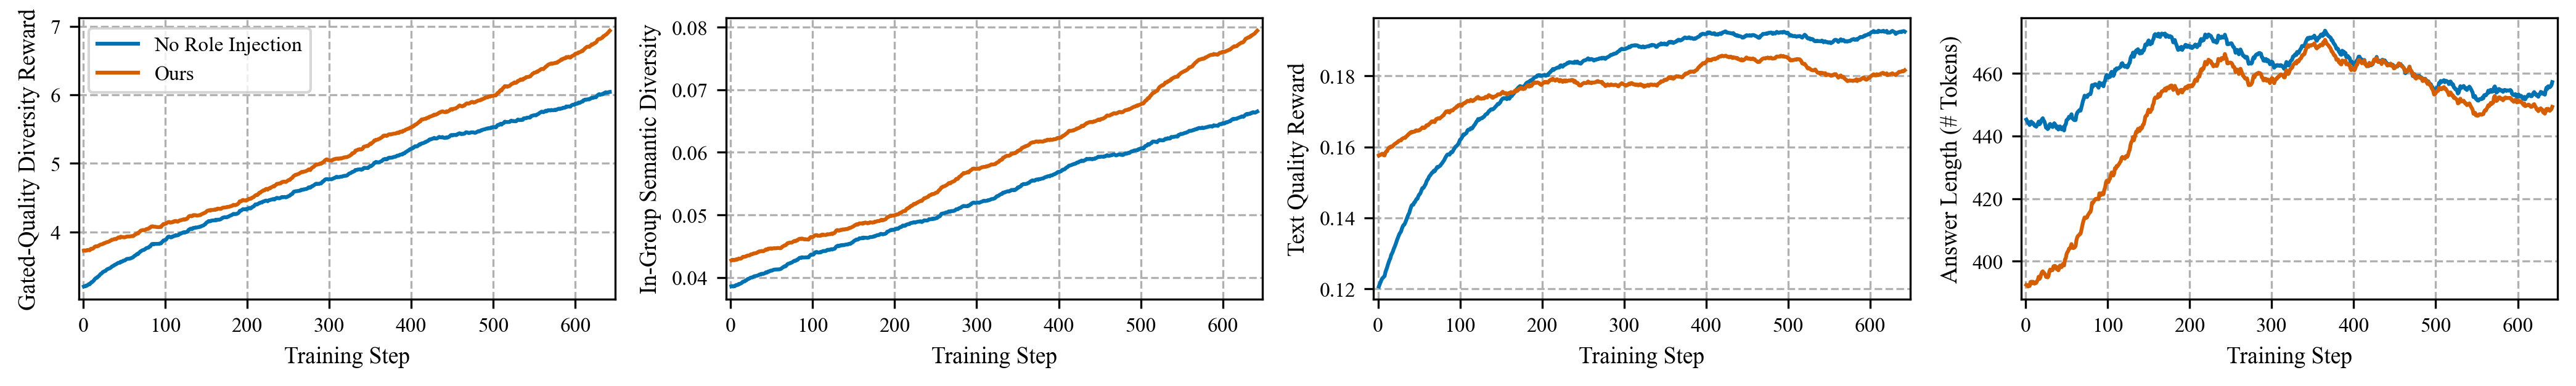
\includegraphics[width=0.82\linewidth]{figures/no_role_wo.png}
    \end{subfigure}
    \caption*{\textbf{No role injection, thinking disabled.}}

    \begin{subfigure}{\textwidth}
        \centering
        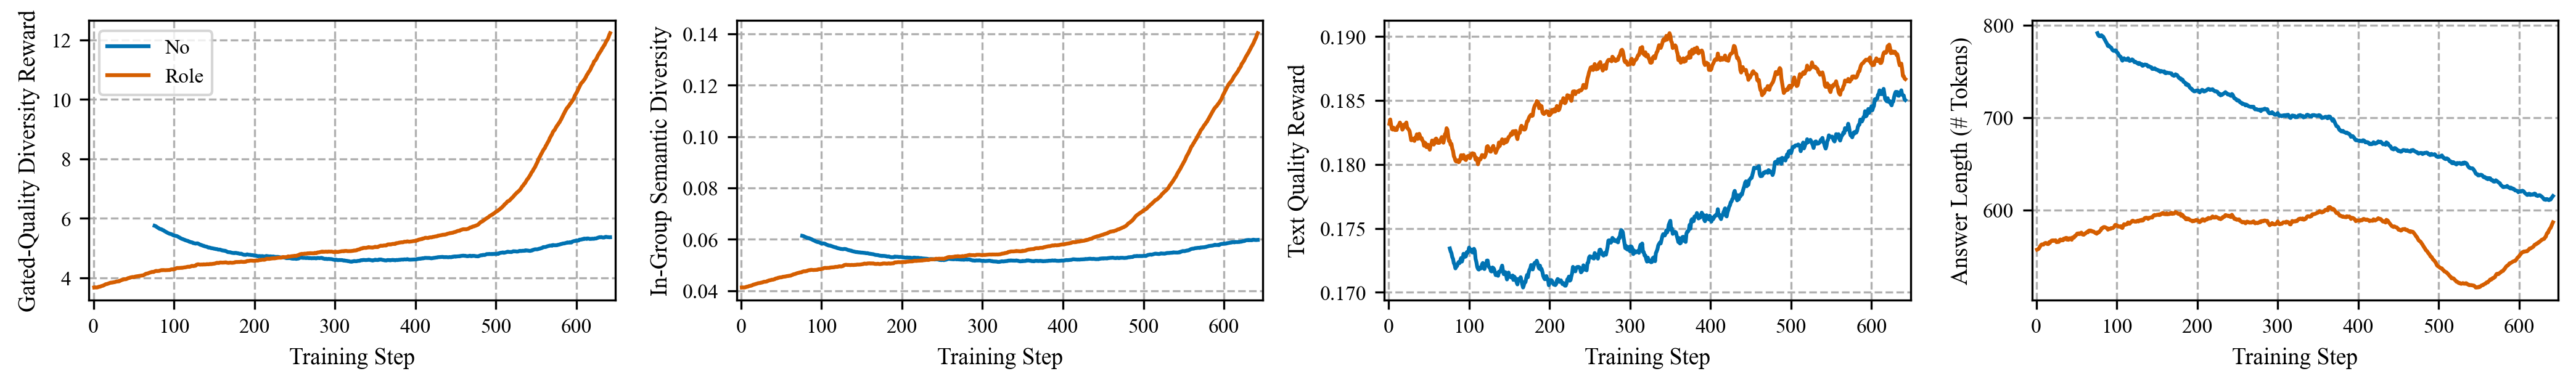
\includegraphics[width=0.82\linewidth]{figures/no_role_w.png}
    \end{subfigure}
    \caption*{\textbf{No role injection, thinking enabled.}}

    \vspace{0.7em}
    % Row 3: Quality-only, thinking disabled
    \begin{subfigure}{\textwidth}
        \centering
        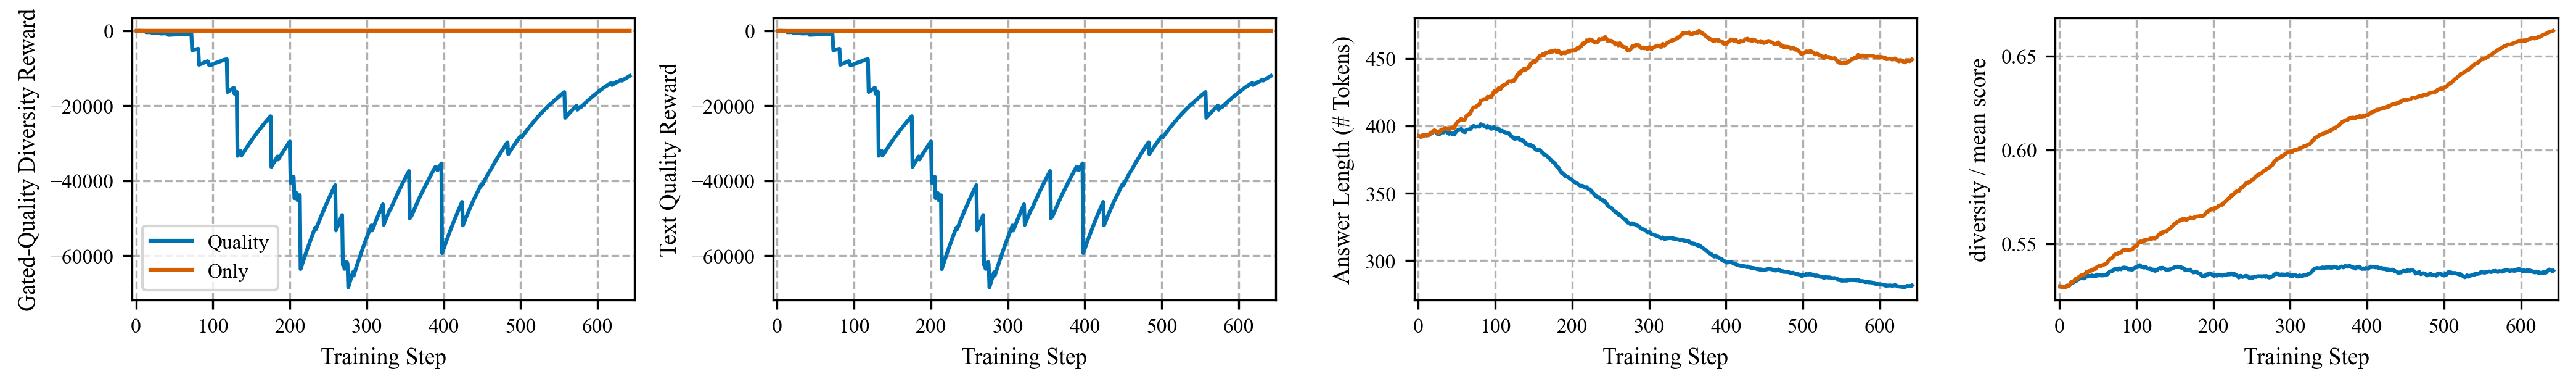
\includegraphics[width=0.82\linewidth]{figures/quality_only_wo.png}
    \end{subfigure}
    \caption*{\textbf{Quality-only reward, thinking disabled.}}

    \vspace{0.7em}

    % Row 4: Quality-only, thinking enabled
    \begin{subfigure}{\textwidth}
        \centering
        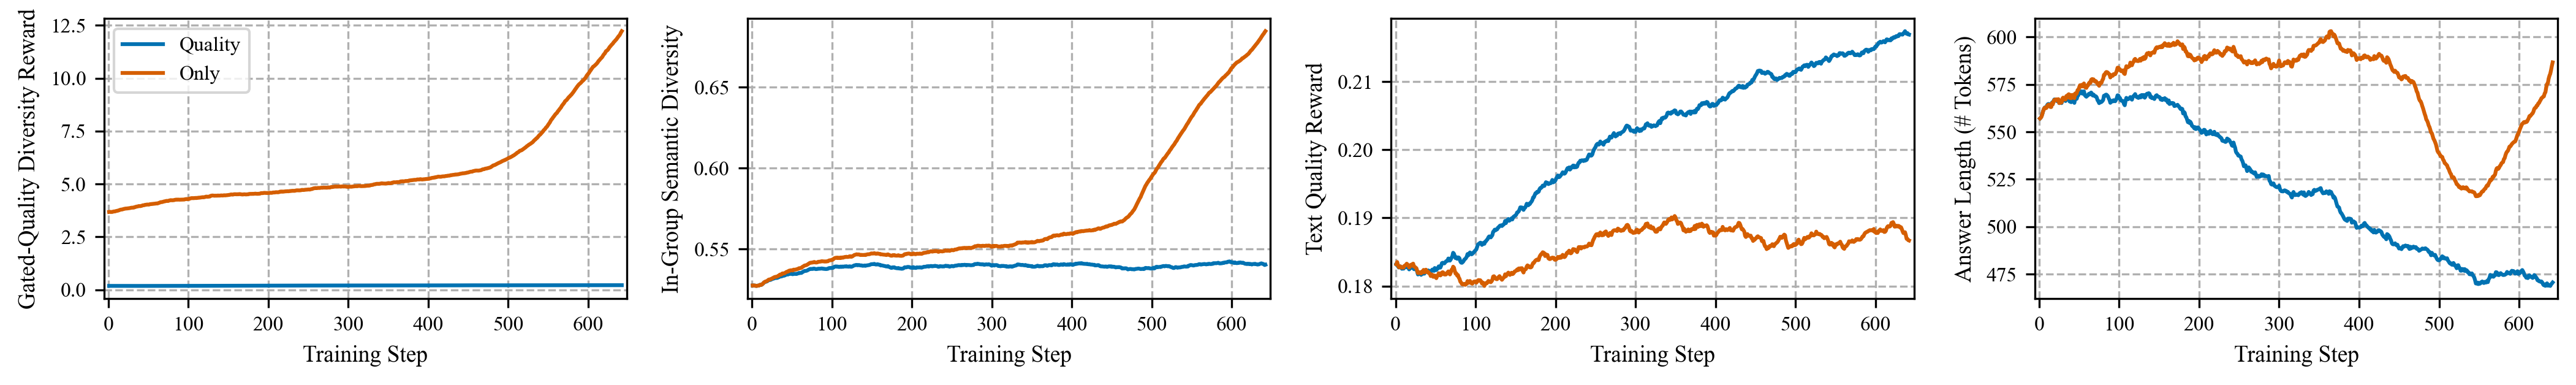
\includegraphics[width=0.82\linewidth]{figures/quality_only_w.png}
    \end{subfigure}
    \caption*{\textbf{Quality-only reward, thinking enabled.}}

     \vspace{0.7em}
    % Row 3: Diversity-only, thinking disabled
    \begin{subfigure}{\textwidth}
        \centering
        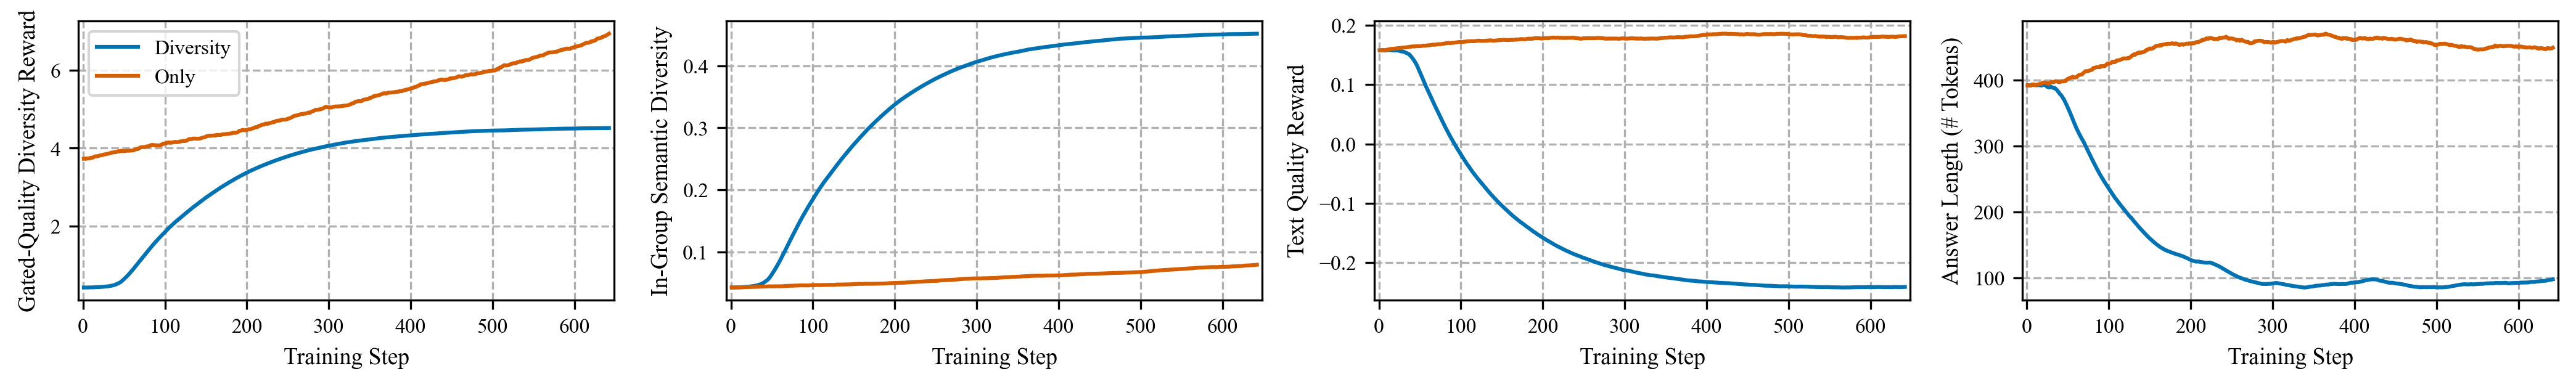
\includegraphics[width=0.82\linewidth]{figures/diversity_only_wo.png}
    \end{subfigure}
    \caption*{\textbf{Diversity-only reward, thinking disabled.}}

    \vspace{0.7em}

    % Row 4: Diversity-only, thinking enabled
    \begin{subfigure}{\textwidth}
        \centering
        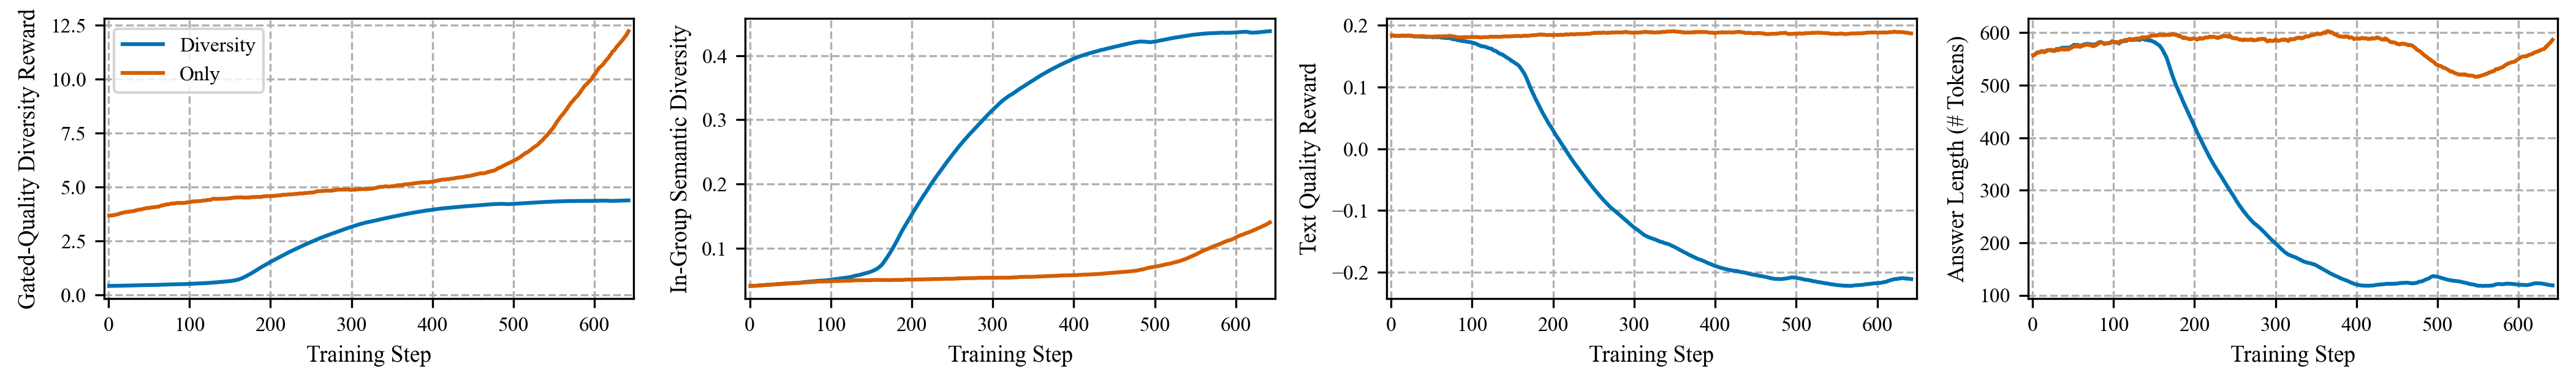
\includegraphics[width=0.82\linewidth]{figures/diversity_only_w.png}
    \end{subfigure}

    \caption*{\textbf{Diversity-only reward, thinking enabled.}}

    % Row 3: Crafted role, thinking disabled
    \begin{subfigure}{\textwidth}
        \centering
        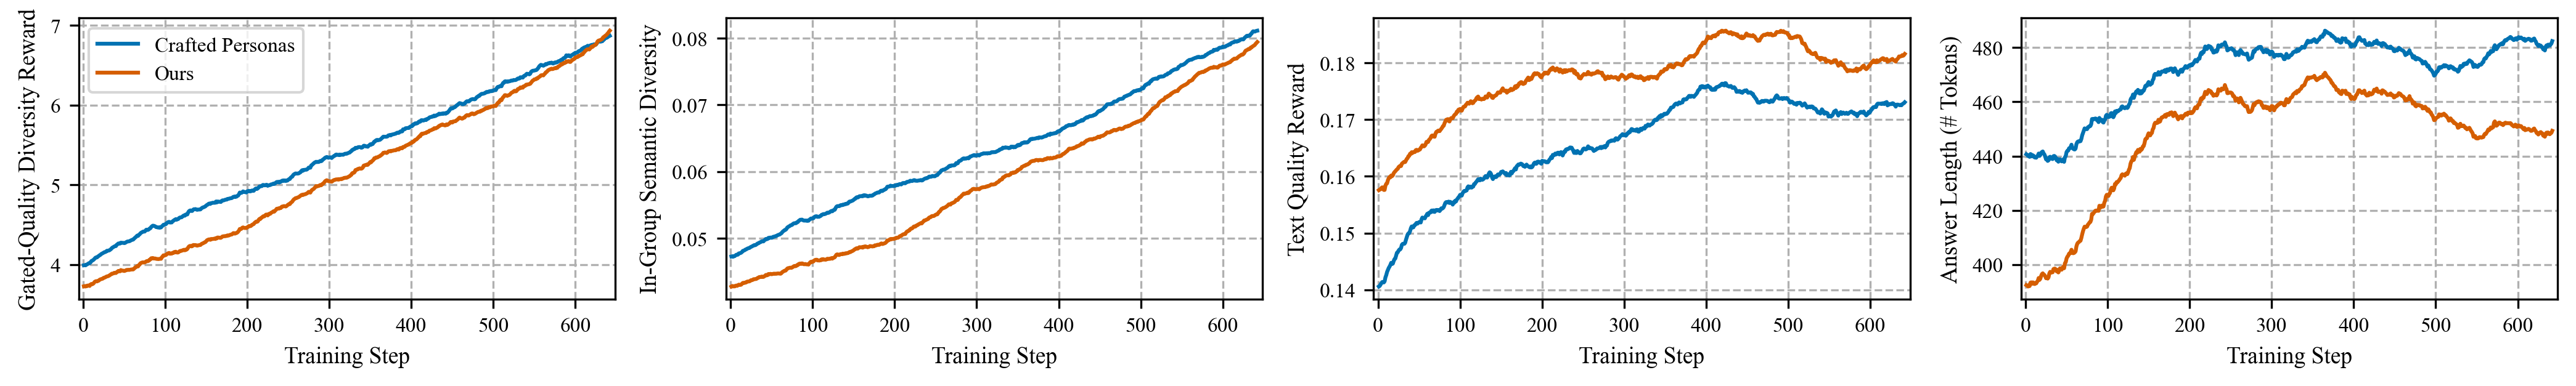
\includegraphics[width=0.82\linewidth]{figures/crafted_wo.png}
    \end{subfigure}
    \caption*{\textbf{Crafted personas, thinking disabled.}}

    \vspace{0.7em}

    % Row 4: Crafted role, thinking enabled
    \begin{subfigure}{\textwidth}
        \centering
        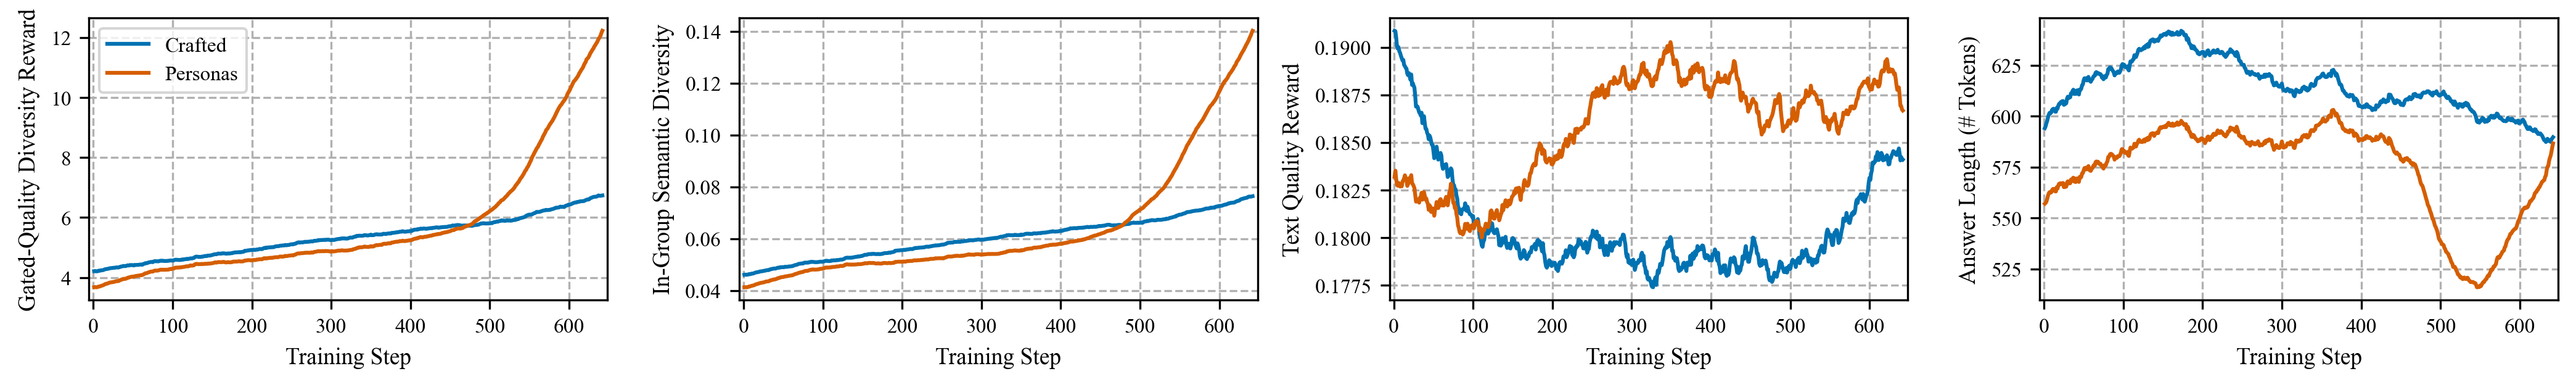
\includegraphics[width=0.82\linewidth]{figures/crafted_w.png}
    \end{subfigure}
    \caption*{\textbf{Crafted personas, thinking enabled.}}



    \caption{
    Training curves for ablation studies. Each row corresponds to one ablation setting, and each row reports four training diagnostics: total reward, diversity reward, quality reward, and answer token length. Results are shown under both thinking-disabled and thinking-enabled settings.}
    \label{fig:ablation-training-curves}
\end{figure}



\newpage
\clearpage


\section{Additional Experiment Results}
\label{appx:additional results}

\subsection{Generative Diversity Evaluation.}
\label{appx:generative diversity evaluation}

\begin{figure}[H]
\centering
\begin{minipage}{0.48\textwidth}
  \centering
  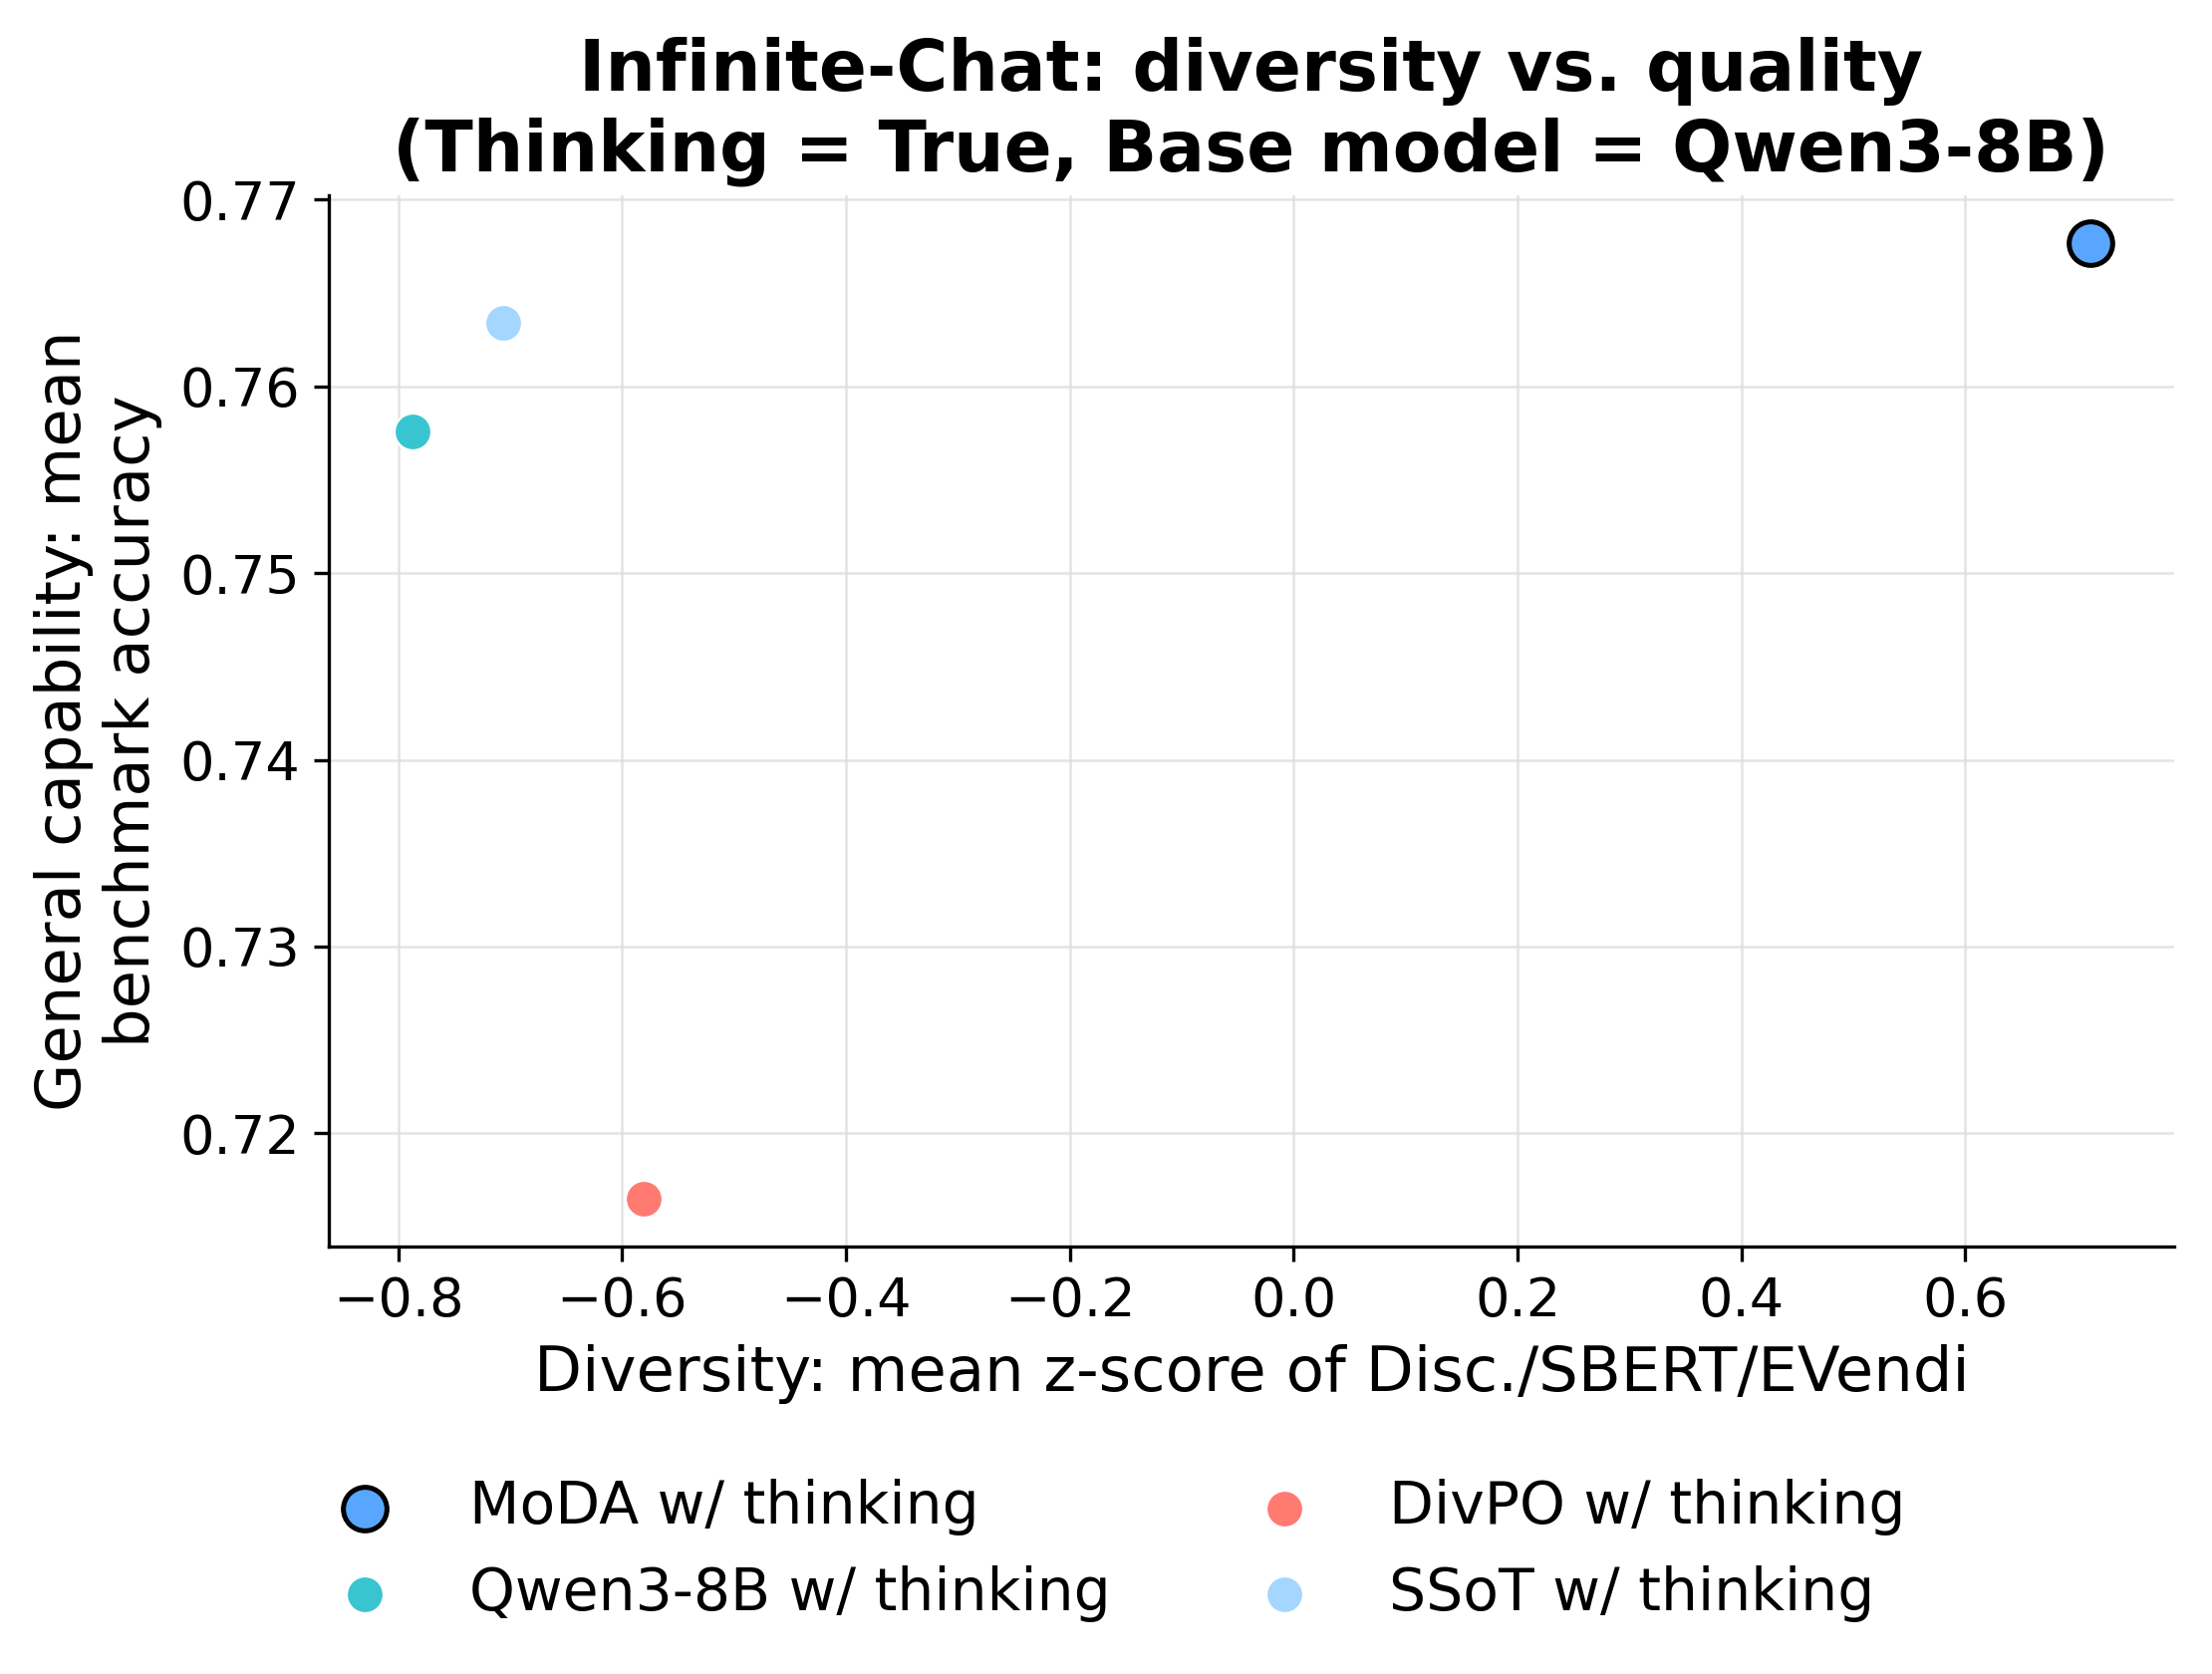
\includegraphics[width=\linewidth]{figures/pareto_infinite-chat_quality_thinking_true_base_model_qwen3-8b_composite.png}
\end{minipage}\hfill
\begin{minipage}{0.48\textwidth}
  \centering
  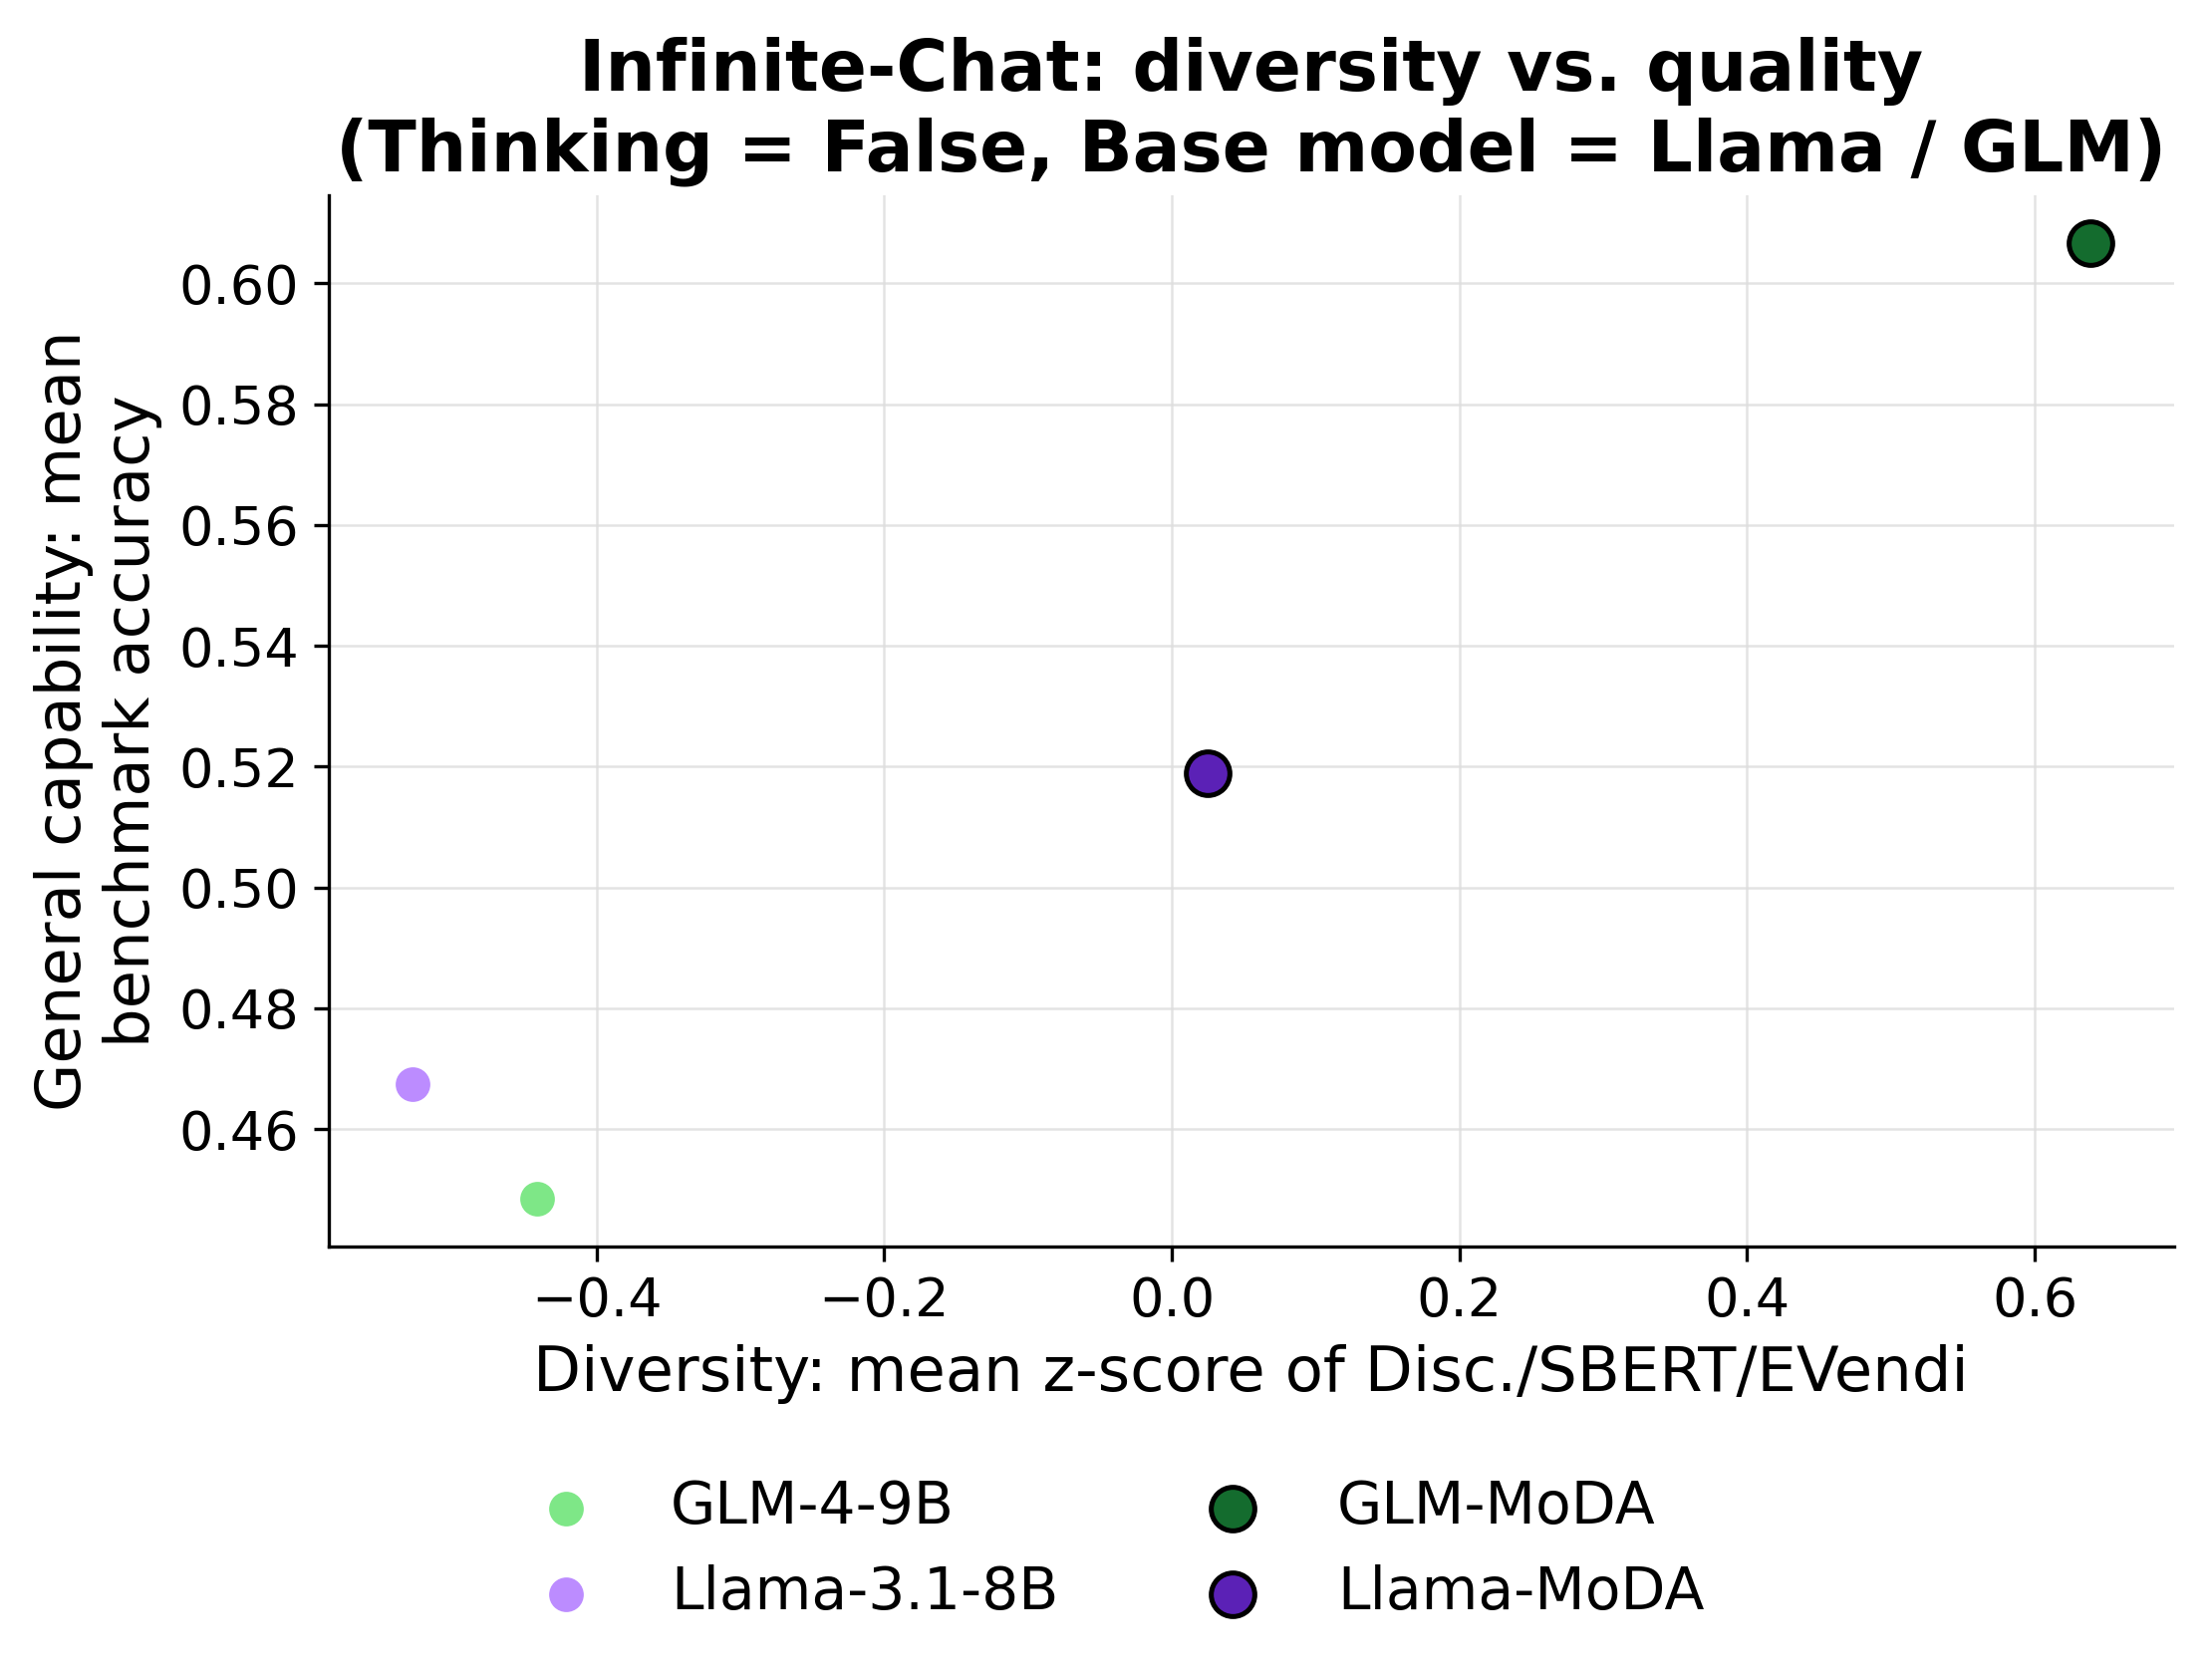
\includegraphics[width=\linewidth]{figures/pareto_infinite-chat_quality_thinking_false_base_model_llama_glm_composite.png}
\end{minipage}
\caption{\textbf{Diversity vs. quality pareto fronts, remaining settings} (extends Figure~\ref{fig: domain application pareto} in the main text). The x-axis is Infinite-Chat response diversity (mean z-score of Disc./SBERT/EmbVendi) and the y-axis is general capability (mean benchmark accuracy). \textbf{Left}: Qwen3-8B base, thinking enabled. \textbf{Right}: Llama-3.1-8B / GLM-4-9B base, thinking disabled. \method{} Pareto-dominates all baselines in both settings.}
\label{fig:domain-application-pareto-appendix}
\end{figure}

We show the results with error bar for generative diversity across all domain application tasks.


\section*{Infinite-Chat}

\begin{table}[H]
\centering
\begin{tabular}{lccccc}
\toprule
Model & Disc. & S & EV & Qual. \\
\midrule
\multicolumn{5}{l}{\textsc{\underline{Qwen3-8B base, thinking disabled}}} \\
Qwen3-8B & 0.400 $\pm$ 0.001 & 0.132 $\pm$ 0.001 & 1.83 $\pm$ 0.01 & 62.9\% $\pm$ 0.8\% \\
DARLING (Mix) & 0.430 $\pm$ 0.001 & 0.203 $\pm$ 0.001 & 2.33 $\pm$ 0.00 & 57.9\% $\pm$ 1.0\% \\
DARLING (WildChat) & 0.416 $\pm$ 0.001 & 0.185 $\pm$ 0.002 & 2.15 $\pm$ 0.01 & 62.7\% $\pm$ 1.0\% \\
DivPO & 0.410 $\pm$ 0.001 & 0.274 $\pm$ 0.004 & 2.86 $\pm$ 0.03 & 66.2\% $\pm$ 0.9\% \\
\method & \textbf{0.472} $\pm$ 0.001 & \textbf{0.482} $\pm$ 0.003 & \textbf{4.40} $\pm$ 0.01 & \textbf{73.2\%} $\pm$ 0.9\% \\
\midrule
\multicolumn{5}{l}{\textsc{\underline{Qwen3-8B base, thinking enabled}}} \\
Qwen3-8B & 0.400 $\pm$ 0.001 & 0.136 $\pm$ 0.001 & 1.85 $\pm$ 0.01 & 75.8\% $\pm$ 0.7\% \\
SSoT & 0.397 $\pm$ 0.000 & 0.178 $\pm$ 0.002 & 2.09 $\pm$ 0.01 & 76.3\% $\pm$ 0.7\% \\
DivPO & 0.414 $\pm$ 0.002 & 0.200 $\pm$ 0.006 & 2.20 $\pm$ 0.03 & 71.7\% $\pm$ 0.8\% \\
\method & \textbf{0.600} $\pm$ 0.001 & \textbf{0.909} $\pm$ 0.001 & \textbf{9.04} $\pm$ 0.01 & \textbf{76.8\%} $\pm$ 0.7\% \\
\midrule
\multicolumn{5}{l}{\textsc{\underline{Llama-3.1-8B base, thinking disabled}}} \\
Llama-3.1-8B & 0.414 $\pm$ 0.001 & 0.217 $\pm$ 0.002 & 2.40 $\pm$ 0.01 & 46.7\% $\pm$ 0.7\% \\
\method{} (Llama-3.1-8B) & \textbf{0.441} $\pm$ 0.002 & \textbf{0.373} $\pm$ 0.003 & \textbf{3.77} $\pm$ 0.02 & \textbf{51.9\%} $\pm$ 0.9\% \\
\midrule
\multicolumn{5}{l}{\textsc{\underline{GLM-4-9B base, thinking disabled}}} \\
GLM-4-9B & 0.421 $\pm$ 0.001 & 0.234 $\pm$ 0.002 & 2.60 $\pm$ 0.01 & 44.9\% $\pm$ 0.9\% \\
\method{}(GLM-4-9b) & \textbf{0.481} $\pm$ 0.001 & \textbf{0.528} $\pm$ 0.001 & \textbf{5.14} $\pm$ 0.01 & \textbf{60.7\%} $\pm$ 0.8\% \\
\bottomrule
\end{tabular}
\end{table}



\section*{NoveltyBench}

\begin{table}[H]
\centering
\begin{tabular}{lccccc}
\toprule
Model & Disc. & S & EV & Qual. \\
\midrule
\multicolumn{5}{l}{\textsc{\underline{Qwen3-8B base, thinking disabled}}} \\
Qwen3-8B & 0.493 $\pm$ 0.002 & 0.224 $\pm$ 0.003 & 2.36 $\pm$ 0.02 & 4.58 $\pm$ 0.04 \\
DARLING (Mix) & 0.513 $\pm$ 0.001 & 0.281 $\pm$ 0.001 & 2.96 $\pm$ 0.01 & 5.24 $\pm$ 0.07 \\
DARLING (WildChat) & 0.480 $\pm$ 0.001 & 0.335 $\pm$ 0.004 & 3.11 $\pm$ 0.02 & 4.00 $\pm$ 0.06 \\
DivPO & 0.519 $\pm$ 0.001 & 0.380 $\pm$ 0.003 & 3.58 $\pm$ 0.02 & 4.87 $\pm$ 0.02 \\
\method & \textbf{0.537} $\pm$ 0.001 & \textbf{0.470} $\pm$ 0.003 & \textbf{4.19} $\pm$ 0.01 & \textbf{5.47} $\pm$ 0.03 \\
\midrule
\multicolumn{5}{l}{\textsc{\underline{Qwen3-8B base, thinking enabled}}} \\
Qwen3-8B & 0.510 $\pm$ 0.001 & 0.258 $\pm$ 0.003 & 2.67 $\pm$ 0.03 & 4.90 $\pm$ 0.04 \\
SSoT & 0.438 $\pm$ 0.001 & 0.239 $\pm$ 0.002 & 2.57 $\pm$ 0.01 & 0.46 $\pm$ 0.01 \\
DivPO & 0.521 $\pm$ 0.001 & 0.327 $\pm$ 0.003 & 3.12 $\pm$ 0.02 & \textbf{5.06} $\pm$ 0.04 \\
\method & \textbf{0.589} $\pm$ 0.002 & \textbf{0.800} $\pm$ 0.004 & \textbf{7.63} $\pm$ 0.07 & 3.39 $\pm$ 0.05 \\
\midrule
\multicolumn{5}{l}{\textsc{\underline{Llama-3.1-8B base, thinking disabled}}} \\
Llama-3.1-8B & 0.512 $\pm$ 0.001 & 0.312 $\pm$ 0.001 & 3.04 $\pm$ 0.01 & 4.80 $\pm$ 0.08 \\
\method{} (Llama-3.1-8B) & \textbf{0.532} $\pm$ 0.001 & \textbf{0.392} $\pm$ 0.001 & \textbf{3.75} $\pm$ 0.01 & \textbf{6.17} $\pm$ 0.04 \\
\midrule
\multicolumn{5}{l}{\textsc{\underline{GLM-4-9B base, thinking disabled}}} \\
GLM-4-9B & \textbf{0.544} $\pm$ 0.002 & 0.408 $\pm$ 0.004 & 4.08 $\pm$ 0.04 & \textbf{4.14} $\pm$ 0.01 \\
\method{}(GLM-4-9b) & 0.502 $\pm$ 0.002 & \textbf{0.521} $\pm$ 0.005 & \textbf{5.01} $\pm$ 0.04 & 2.70 $\pm$ 0.03 \\
\bottomrule
\end{tabular}
\end{table}



\section*{HypoBench}

\begin{table}[H]
\centering
\begin{tabular}{lccccc}
\toprule
Model & Disc. & S & EV & Qual. \\
\midrule
\multicolumn{5}{l}{\textsc{\underline{Qwen3-8B base, thinking disabled}}} \\
Qwen3-8B & 0.384 $\pm$ 0.005 & 0.144 $\pm$ 0.005 & 1.91 $\pm$ 0.03 & \textbf{4.03} $\pm$ 0.01 \\
DARLING (Mix) & 0.406 $\pm$ 0.005 & 0.222 $\pm$ 0.004 & 2.48 $\pm$ 0.02 & 3.44 $\pm$ 0.03 \\
DARLING (WildChat) & 0.415 $\pm$ 0.004 & 0.205 $\pm$ 0.006 & 2.34 $\pm$ 0.04 & 3.73 $\pm$ 0.02 \\
DivPO & 0.427 $\pm$ 0.006 & 0.198 $\pm$ 0.005 & 2.30 $\pm$ 0.03 & 3.89 $\pm$ 0.01 \\
\method & \textbf{0.480} $\pm$ 0.003 & \textbf{0.547} $\pm$ 0.010 & \textbf{4.91} $\pm$ 0.05 & 3.80 $\pm$ 0.02 \\
\midrule
\multicolumn{5}{l}{\textsc{\underline{Qwen3-8B base, thinking enabled}}} \\
Qwen3-8B & 0.399 $\pm$ 0.006 & 0.164 $\pm$ 0.005 & 2.05 $\pm$ 0.03 & \textbf{3.93} $\pm$ 0.01 \\
SSoT & 0.419 $\pm$ 0.002 & 0.220 $\pm$ 0.010 & 2.33 $\pm$ 0.04 & 3.75 $\pm$ 0.02 \\
DivPO & 0.409 $\pm$ 0.002 & 0.162 $\pm$ 0.005 & 2.04 $\pm$ 0.03 & 3.89 $\pm$ 0.01 \\
\method & \textbf{0.579} $\pm$ 0.013 & \textbf{0.875} $\pm$ 0.018 & \textbf{8.06} $\pm$ 0.25 & 3.71 $\pm$ 0.04 \\
\midrule
\multicolumn{5}{l}{\textsc{\underline{Llama-3.1-8B base, thinking disabled}}} \\
Llama-3.1-8B & \textbf{0.469} $\pm$ 0.005 & 0.207 $\pm$ 0.006 & 2.38 $\pm$ 0.04 & 3.60 $\pm$ 0.02 \\
\method{} (Llama-3.1-8B) & 0.410 $\pm$ 0.001 & \textbf{0.324} $\pm$ 0.014 & \textbf{3.27} $\pm$ 0.10 & \textbf{3.65} $\pm$ 0.01 \\
\midrule
\multicolumn{5}{l}{\textsc{\underline{GLM-4-9B base, thinking disabled}}} \\
GLM-4-9B & 0.402 $\pm$ 0.003 & 0.225 $\pm$ 0.005 & 2.52 $\pm$ 0.03 & \textbf{3.75} $\pm$ 0.01 \\
\method{}(GLM-4-9b) & \textbf{0.452} $\pm$ 0.003 & \textbf{0.485} $\pm$ 0.012 & \textbf{4.64} $\pm$ 0.09 & 3.68 $\pm$ 0.01 \\
\bottomrule
\end{tabular}
\end{table}


\section*{PreScience}

\begin{table}[H]
\centering
\begin{tabular}{lccccc}
\toprule
Model & Disc. & S & EV & Qual. \\
\midrule
\multicolumn{5}{l}{\textsc{\underline{Qwen3-8B base, thinking disabled}}} \\
Qwen3-8B & 0.431 $\pm$ 0.002 & 0.155 $\pm$ 0.004 & 1.94 $\pm$ 0.02 & \textbf{4.25} $\pm$ 0.03 \\
DARLING (Mix) & \textbf{0.559} $\pm$ 0.005 & \textbf{0.541} $\pm$ 0.018 & \textbf{4.73} $\pm$ 0.15 & 2.33 $\pm$ 0.07 \\
DARLING (WildChat) & 0.446 $\pm$ 0.002 & 0.192 $\pm$ 0.003 & 2.21 $\pm$ 0.03 & 4.03 $\pm$ 0.06 \\
DivPO & 0.455 $\pm$ 0.002 & 0.233 $\pm$ 0.001 & 2.41 $\pm$ 0.01 & 3.96 $\pm$ 0.05 \\
\method & 0.440 $\pm$ 0.002 & 0.176 $\pm$ 0.002 & 2.10 $\pm$ 0.01 & 3.96 $\pm$ 0.01 \\
\midrule
\multicolumn{5}{l}{\textsc{\underline{Qwen3-8B base, thinking enabled}}} \\
Qwen3-8B & 0.441 $\pm$ 0.003 & 0.136 $\pm$ 0.001 & 1.83 $\pm$ 0.01 & 3.79 $\pm$ 0.04 \\
SSoT & \textbf{0.461} $\pm$ 0.002 & \textbf{0.281} $\pm$ 0.017 & \textbf{2.39} $\pm$ 0.05 & 3.30 $\pm$ 0.05 \\
DivPO & 0.448 $\pm$ 0.003 & 0.185 $\pm$ 0.015 & 2.04 $\pm$ 0.07 & \textbf{3.87} $\pm$ 0.06 \\
\method & 0.439 $\pm$ 0.001 & 0.194 $\pm$ 0.005 & 2.10 $\pm$ 0.01 & 3.68 $\pm$ 0.00 \\
\midrule
\multicolumn{5}{l}{\textsc{\underline{Llama-3.1-8B base, thinking disabled}}} \\
Llama-3.1-8B & 0.461 $\pm$ 0.005 & \textbf{0.514} $\pm$ 0.020 & 3.67 $\pm$ 0.07 & \textbf{2.62} $\pm$ 0.05 \\
\method{} (Llama-3.1-8B) & \textbf{0.472} $\pm$ 0.003 & 0.470 $\pm$ 0.009 & \textbf{3.89} $\pm$ 0.07 & 2.54 $\pm$ 0.04 \\
\midrule
\multicolumn{5}{l}{\textsc{\underline{GLM-4-9B base, thinking disabled}}} \\
GLM-4-9B & 0.461 $\pm$ 0.004 & 0.438 $\pm$ 0.010 & 4.15 $\pm$ 0.08 & 2.57 $\pm$ 0.05 \\
\method{}(GLM-4-9b) & \textbf{0.464} $\pm$ 0.002 & \textbf{0.448} $\pm$ 0.010 & \textbf{4.28} $\pm$ 0.09 & \textbf{2.58} $\pm$ 0.10 \\
\bottomrule
\end{tabular}
\end{table}

\subsection{General Capability Retention}
\label{appx:general capability retention}

\subsubsection{Pass@1}
We show general capability retention with error bar for pass@1 across baselines and our model.
\begin{table}[H]
\setlength{\tabcolsep}{2.5pt}
\centering
\small
\begin{tabular}{lcccccccc}
\toprule
Model & GSM8K & MMLU & GPQA & BoolQ & HellaSwag & TruthfulQA & IFEval & Avg. \\
\midrule
\multicolumn{9}{l}{\textsc{\underline{Qwen3-8B base, thinking disabled}}} \\
Qwen3-8B & 84.5 $\pm$ 1.0 & \textbf{82.0} $\pm$ 3.9 & 41.4 $\pm$ 3.5 & 83.1 $\pm$ 0.7 & 48.4 $\pm$ 0.5 & 22.2 $\pm$ 1.5 & \textbf{78.4} $\pm$ 1.8 & 62.9 $\pm$ 0.8 \\
DARLING (Mixture) & 63.5 $\pm$ 1.3 & 63.0 $\pm$ 4.9 & 34.3 $\pm$ 3.4 & 76.7 $\pm$ 0.7 & 62.2 $\pm$ 0.5 & 52.4 $\pm$ 1.7 & 53.0 $\pm$ 2.1 & 57.9 $\pm$ 1.0 \\
DARLING (WildChat) & 77.9 $\pm$ 1.1 & 55.0 $\pm$ 5.0 & 34.3 $\pm$ 3.4 & \textbf{86.4} $\pm$ 0.6 & 68.8 $\pm$ 0.5 & 43.2 $\pm$ 1.7 & 73.0 $\pm$ 1.9 & 62.7 $\pm$ 1.0 \\
DivPO & 80.5 $\pm$ 1.1 & 81.0 $\pm$ 3.9 & 40.4 $\pm$ 3.5 & 83.5 $\pm$ 0.6 & 62.8 $\pm$ 0.5 & 37.7 $\pm$ 1.7 & 77.3 $\pm$ 1.8 & 66.2 $\pm$ 0.9 \\
\method & \textbf{86.7} $\pm$ 0.9 & 81.0 $\pm$ 3.9 & \textbf{52.0} $\pm$ 3.6 & 84.8 $\pm$ 0.6 & \textbf{73.4} $\pm$ 0.4 & \textbf{57.9} $\pm$ 1.7 & 76.9 $\pm$ 1.8 & \textbf{73.2} $\pm$ 0.9 \\
\midrule
\multicolumn{9}{l}{\textsc{\underline{Qwen3-8B base, thinking enabled}}} \\
Qwen3-8B & \textbf{90.3} $\pm$ 0.8 & \textbf{94.0} $\pm$ 2.4 & 43.4 $\pm$ 3.5 & \textbf{87.2} $\pm$ 0.6 & 70.9 $\pm$ 0.5 & 64.9 $\pm$ 1.7 & \textbf{79.7} $\pm$ 1.7 & 75.8 $\pm$ 0.7 \\
SSoT & 84.3 $\pm$ 1.0 & 93.0 $\pm$ 2.6 & \textbf{55.1} $\pm$ 3.5 & \textbf{87.2} $\pm$ 0.6 & \textbf{80.1} $\pm$ 0.4 & \textbf{72.8} $\pm$ 1.6 & 61.9 $\pm$ 2.1 & 76.3 $\pm$ 0.7 \\
DivPO & 84.9 $\pm$ 1.0 & 91.0 $\pm$ 2.9 & 44.4 $\pm$ 3.5 & 83.2 $\pm$ 0.7 & 65.0 $\pm$ 0.5 & 55.3 $\pm$ 1.7 & 77.6 $\pm$ 1.8 & 71.7 $\pm$ 0.8 \\
\method & 83.9 $\pm$ 1.0 & 93.0 $\pm$ 2.6 & 50.5 $\pm$ 3.6 & \textbf{87.2} $\pm$ 0.6 & 76.2 $\pm$ 0.4 & 67.2 $\pm$ 1.6 & 79.5 $\pm$ 1.7 & \textbf{76.8} $\pm$ 0.7 \\
\midrule
\multicolumn{9}{l}{\textsc{\underline{Llama-3.1-8B base, thinking disabled}}} \\
Llama-3.1-8B & 71.3 $\pm$ 1.2 & 16.0 $\pm$ 3.7 & 6.1 $\pm$ 1.7 & \textbf{81.6} $\pm$ 0.7 & 30.2 $\pm$ 0.5 & 53.4 $\pm$ 1.7 & 68.8 $\pm$ 2.0 & 46.7 $\pm$ 0.7 \\
\method(Llama-3.1-8B) & \textbf{74.9} $\pm$ 1.2 & \textbf{30.0} $\pm$ 4.6 & \textbf{18.7} $\pm$ 2.8 & 75.6 $\pm$ 0.8 & \textbf{38.5} $\pm$ 0.5 & \textbf{54.7} $\pm$ 1.7 & \textbf{70.8} $\pm$ 2.0 & \textbf{51.9} $\pm$ 0.9 \\
\midrule
\multicolumn{9}{l}{\textsc{\underline{GLM-4-9B base, thinking disabled}}} \\
GLM-4-9B & 21.8 $\pm$ 1.1 & 35.0 $\pm$ 4.8 & 19.7 $\pm$ 2.8 & 74.5 $\pm$ 0.8 & \textbf{68.0} $\pm$ 0.5 & \textbf{44.8} $\pm$ 1.7 & 50.3 $\pm$ 2.2 & 44.9 $\pm$ 0.9 \\
\method(GLM-4-9B) & \textbf{84.9} $\pm$ 1.0 & \textbf{83.0} $\pm$ 3.8 & \textbf{33.3} $\pm$ 3.4 & \textbf{81.2} $\pm$ 0.7 & 52.3 $\pm$ 0.5 & 34.5 $\pm$ 1.7 & \textbf{55.5} $\pm$ 2.1 & \textbf{60.7} $\pm$ 0.8 \\
\bottomrule
\end{tabular}
\vspace{4pt}
\caption{General capability retention (accuracy \%, mean ± std error; bold = best per block)}
\label{tab:general-capability-pass1-error-bar}
\end{table}

\subsubsection{Pass@5}
We show general capability retention for pass@5 across baselines and our model.
\begin{table}[H]
\centering
\small
\setlength{\tabcolsep}{4pt}
\resizebox{\textwidth}{!}{%
\begin{tabular}{lcccccccc}
\toprule
Model & GSM8K & MMLU & GPQA & BoolQ & HellaSwag & TruthfulQA & IFEval & Avg. \\
\midrule
\multicolumn{9}{l}{\textsc{\underline{Qwen3-8B base, thinking disabled}}} \\
Qwen3-8B & 92.6 & 92.0 & 73.7 & 89.7 & 86.0 & 55.1 & 83.4 & 81.8 \\
DARLING (Mixture) & 92.8 & \textbf{95.0} & \textbf{75.3} & 93.1 & 91.2 & 86.4 & 57.3 & 84.4 \\
DARLING (WildChat) & 91.8 & 86.0 & 69.2 & 91.3 & 91.3 & 74.4 & 80.8 & 83.5 \\
DivPO & 92.3 & 92.0 & 74.7 & 93.2 & 90.5 & 76.3 & \textbf{85.6} & 86.4 \\
\method & \textbf{94.5} & 93.0 & 74.7 & \textbf{93.9} & \textbf{91.3} & \textbf{86.5} & 83.9 & \textbf{88.3} \\
\midrule
\multicolumn{9}{l}{\textsc{\underline{Qwen3-8B base, thinking enabled}}} \\
Qwen3-8B & 96.1 & 96.0 & 66.2 & 92.2 & 89.1 & 82.5 & 85.4 & 86.8 \\
SSoT & 90.6 & 96.0 & \textbf{74.7} & 92.0 & 88.9 & \textbf{83.8} & 73.6 & 85.7 \\
DivPO & 94.0 & \textbf{97.0} & 72.2 & \textbf{93.0} & \textbf{89.8} & \textbf{83.8} & 85.6 & \textbf{87.9} \\
\method & \textbf{96.3} & 96.0 & 68.7 & 92.0 & 89.6 & 82.5 & \textbf{85.8} & 87.3 \\
\midrule
\multicolumn{9}{l}{\textsc{\underline{Llama-3.1-8B base, thinking disabled}}} \\
Llama-3.1-8B & 90.1 & 57.0 & 28.3 & \textbf{93.2} & 70.2 & 72.9 & \textbf{82.3} & 70.6 \\
\method(Llama-3.1-8B) & \textbf{93.5} & \textbf{76.0} & \textbf{56.6} & 92.3 & \textbf{79.6} & \textbf{80.4} & 80.2 & \textbf{79.8} \\
\midrule
\multicolumn{9}{l}{\textsc{\underline{GLM-4-9b base, thinking disabled}}} \\
GLM-4-9B & 60.0 & 69.0 & 59.6 & \textbf{97.1} & \textbf{91.3} & \textbf{82.6} & 57.5 & 73.9 \\
\method(GLM-4-9B) & \textbf{95.2} & \textbf{94.0} & \textbf{73.2} & 95.3 & 89.1 & 77.5 & \textbf{74.7} & \textbf{85.6} \\
\bottomrule
\end{tabular}
}
\vspace{4pt}
\caption{General capability retention pass@5. For IFEval, strict instruction-following accuracy is reported. Avg.\ is the row mean across benchmarks. Bold marks the best average within each thinking setting.}
\label{tab:general-capability-pass5}
\end{table}


We show pass@k figures for the rest of the general capability suite tasks below.
\begin{figure}[H]
\centering
\begin{minipage}{0.24\textwidth}
  \centering
  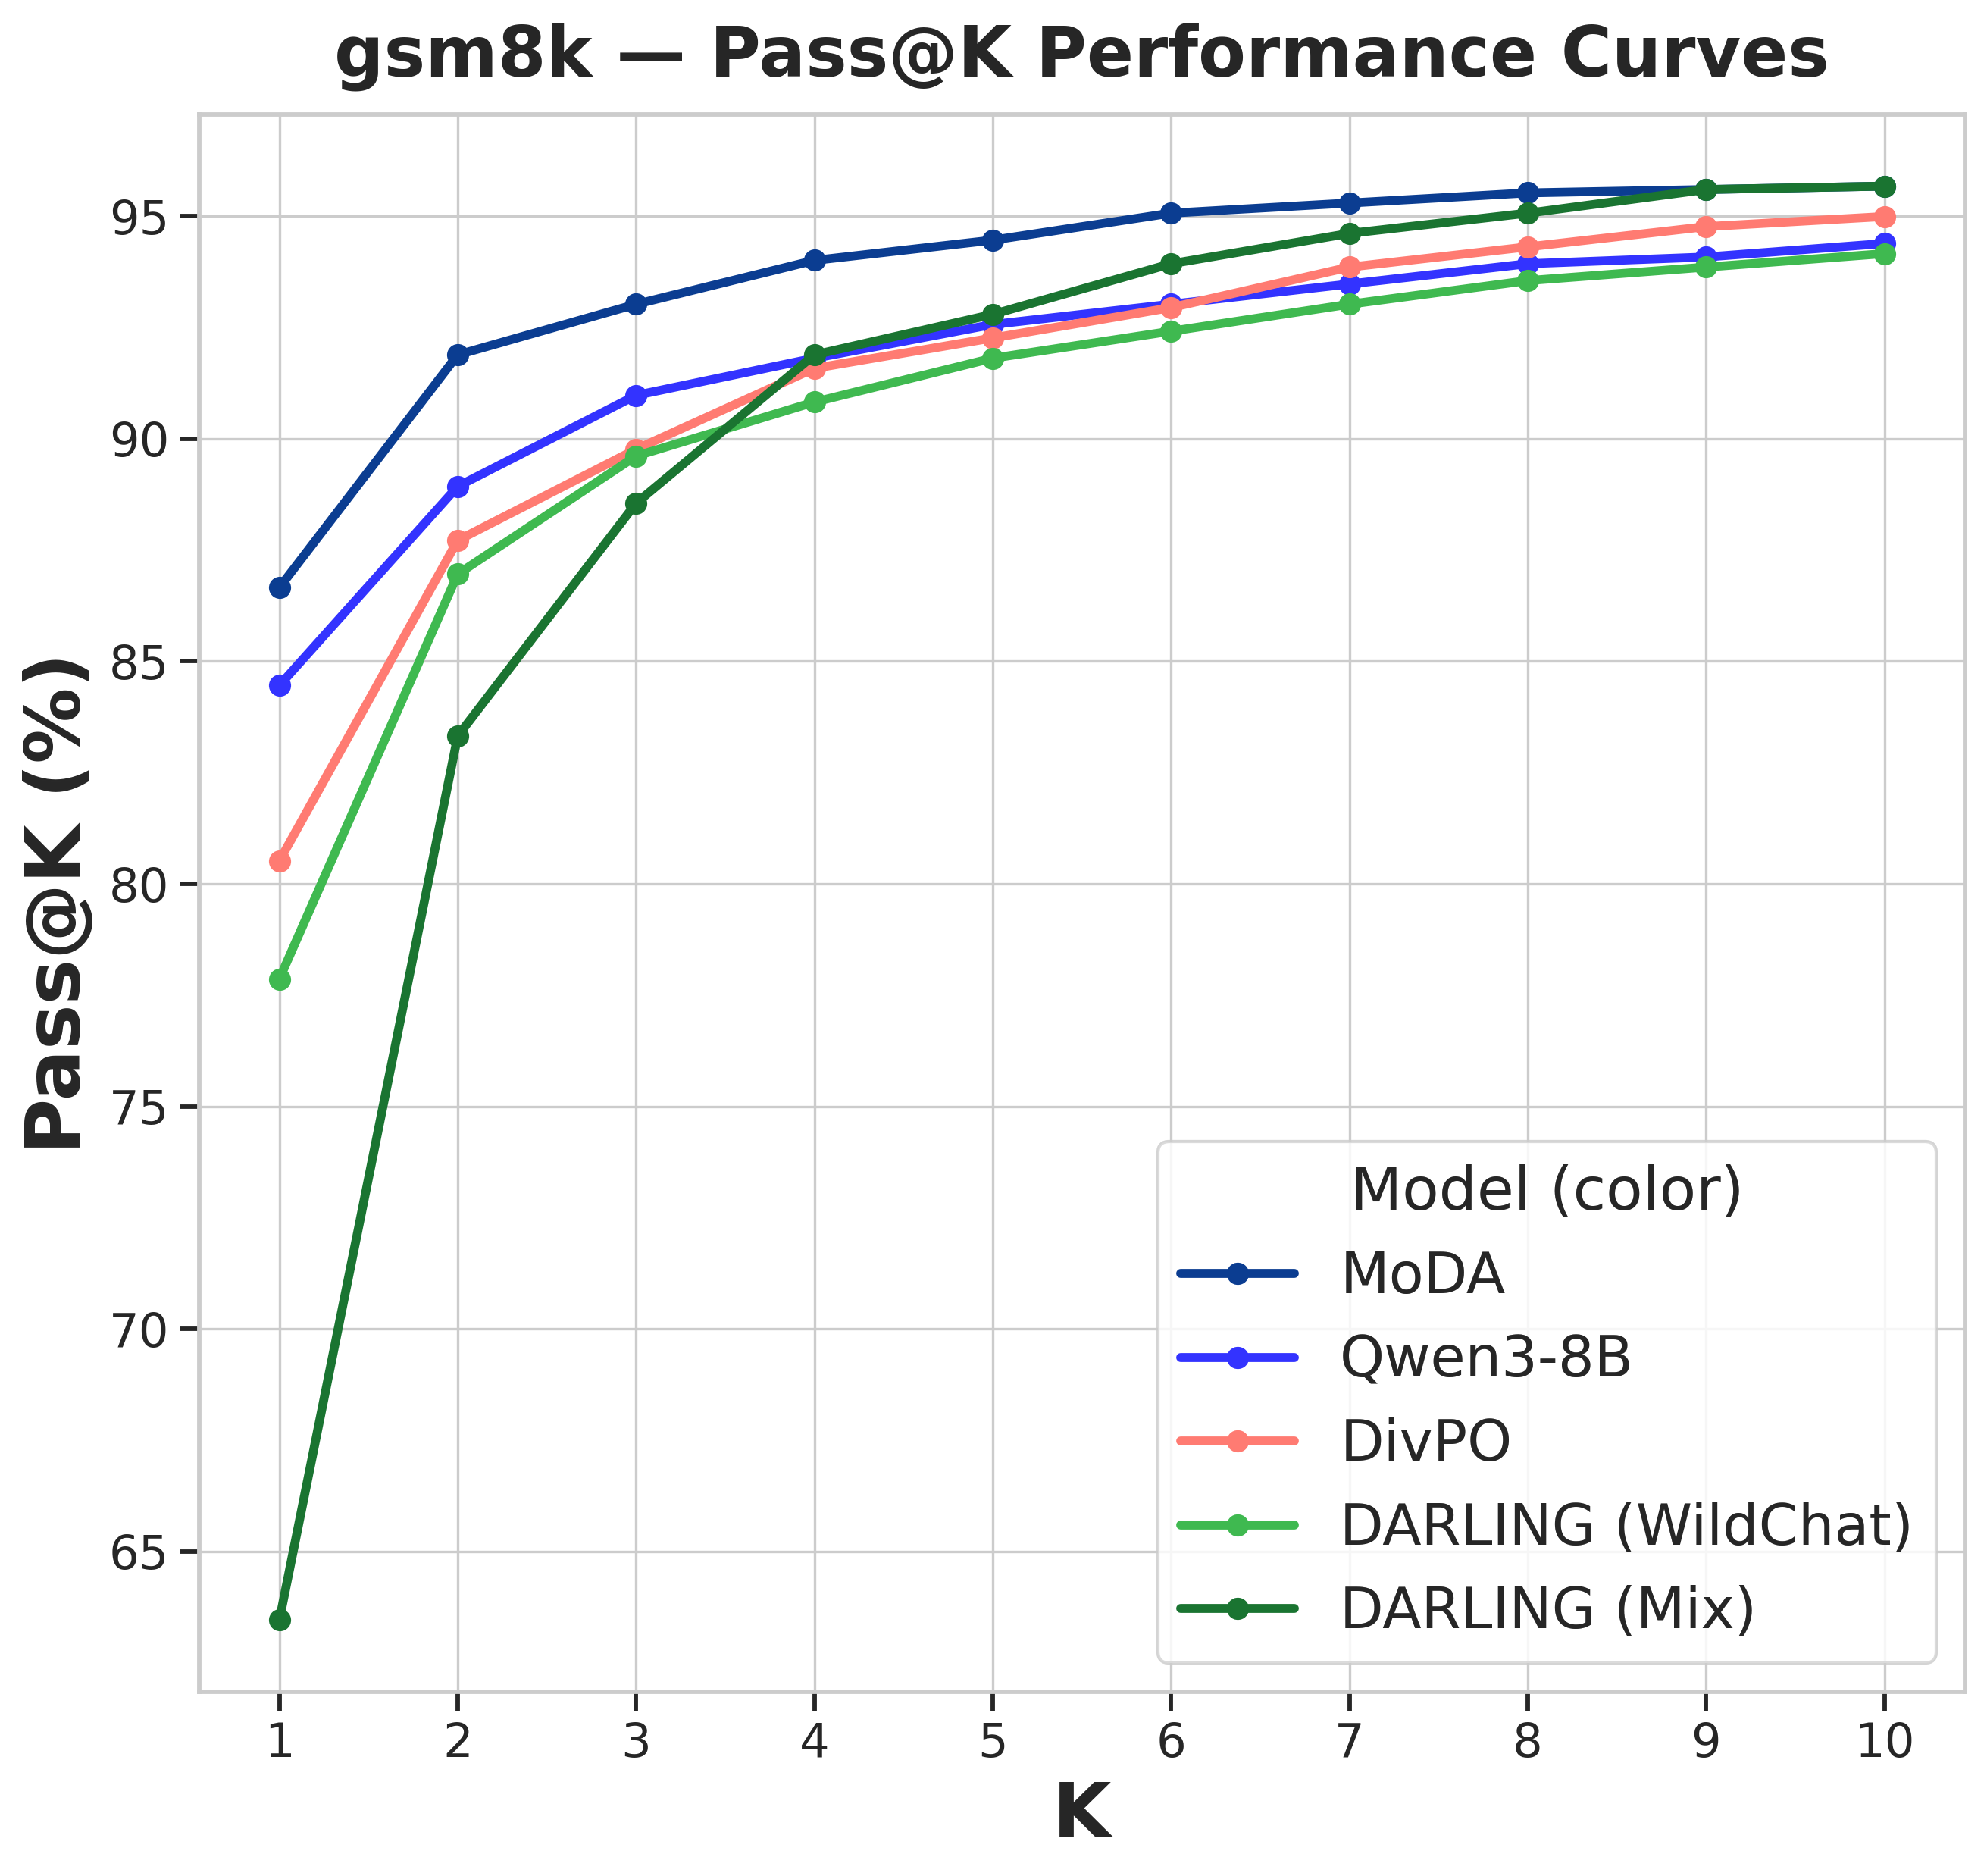
\includegraphics[width=\linewidth]{figures/main_pass_k/pass_at_k_figures/pass_at_k_gsm8k_thinking_false_base_model_qwen3-8b.png}
\end{minipage}\hfill
\begin{minipage}{0.24\textwidth}
  \centering
  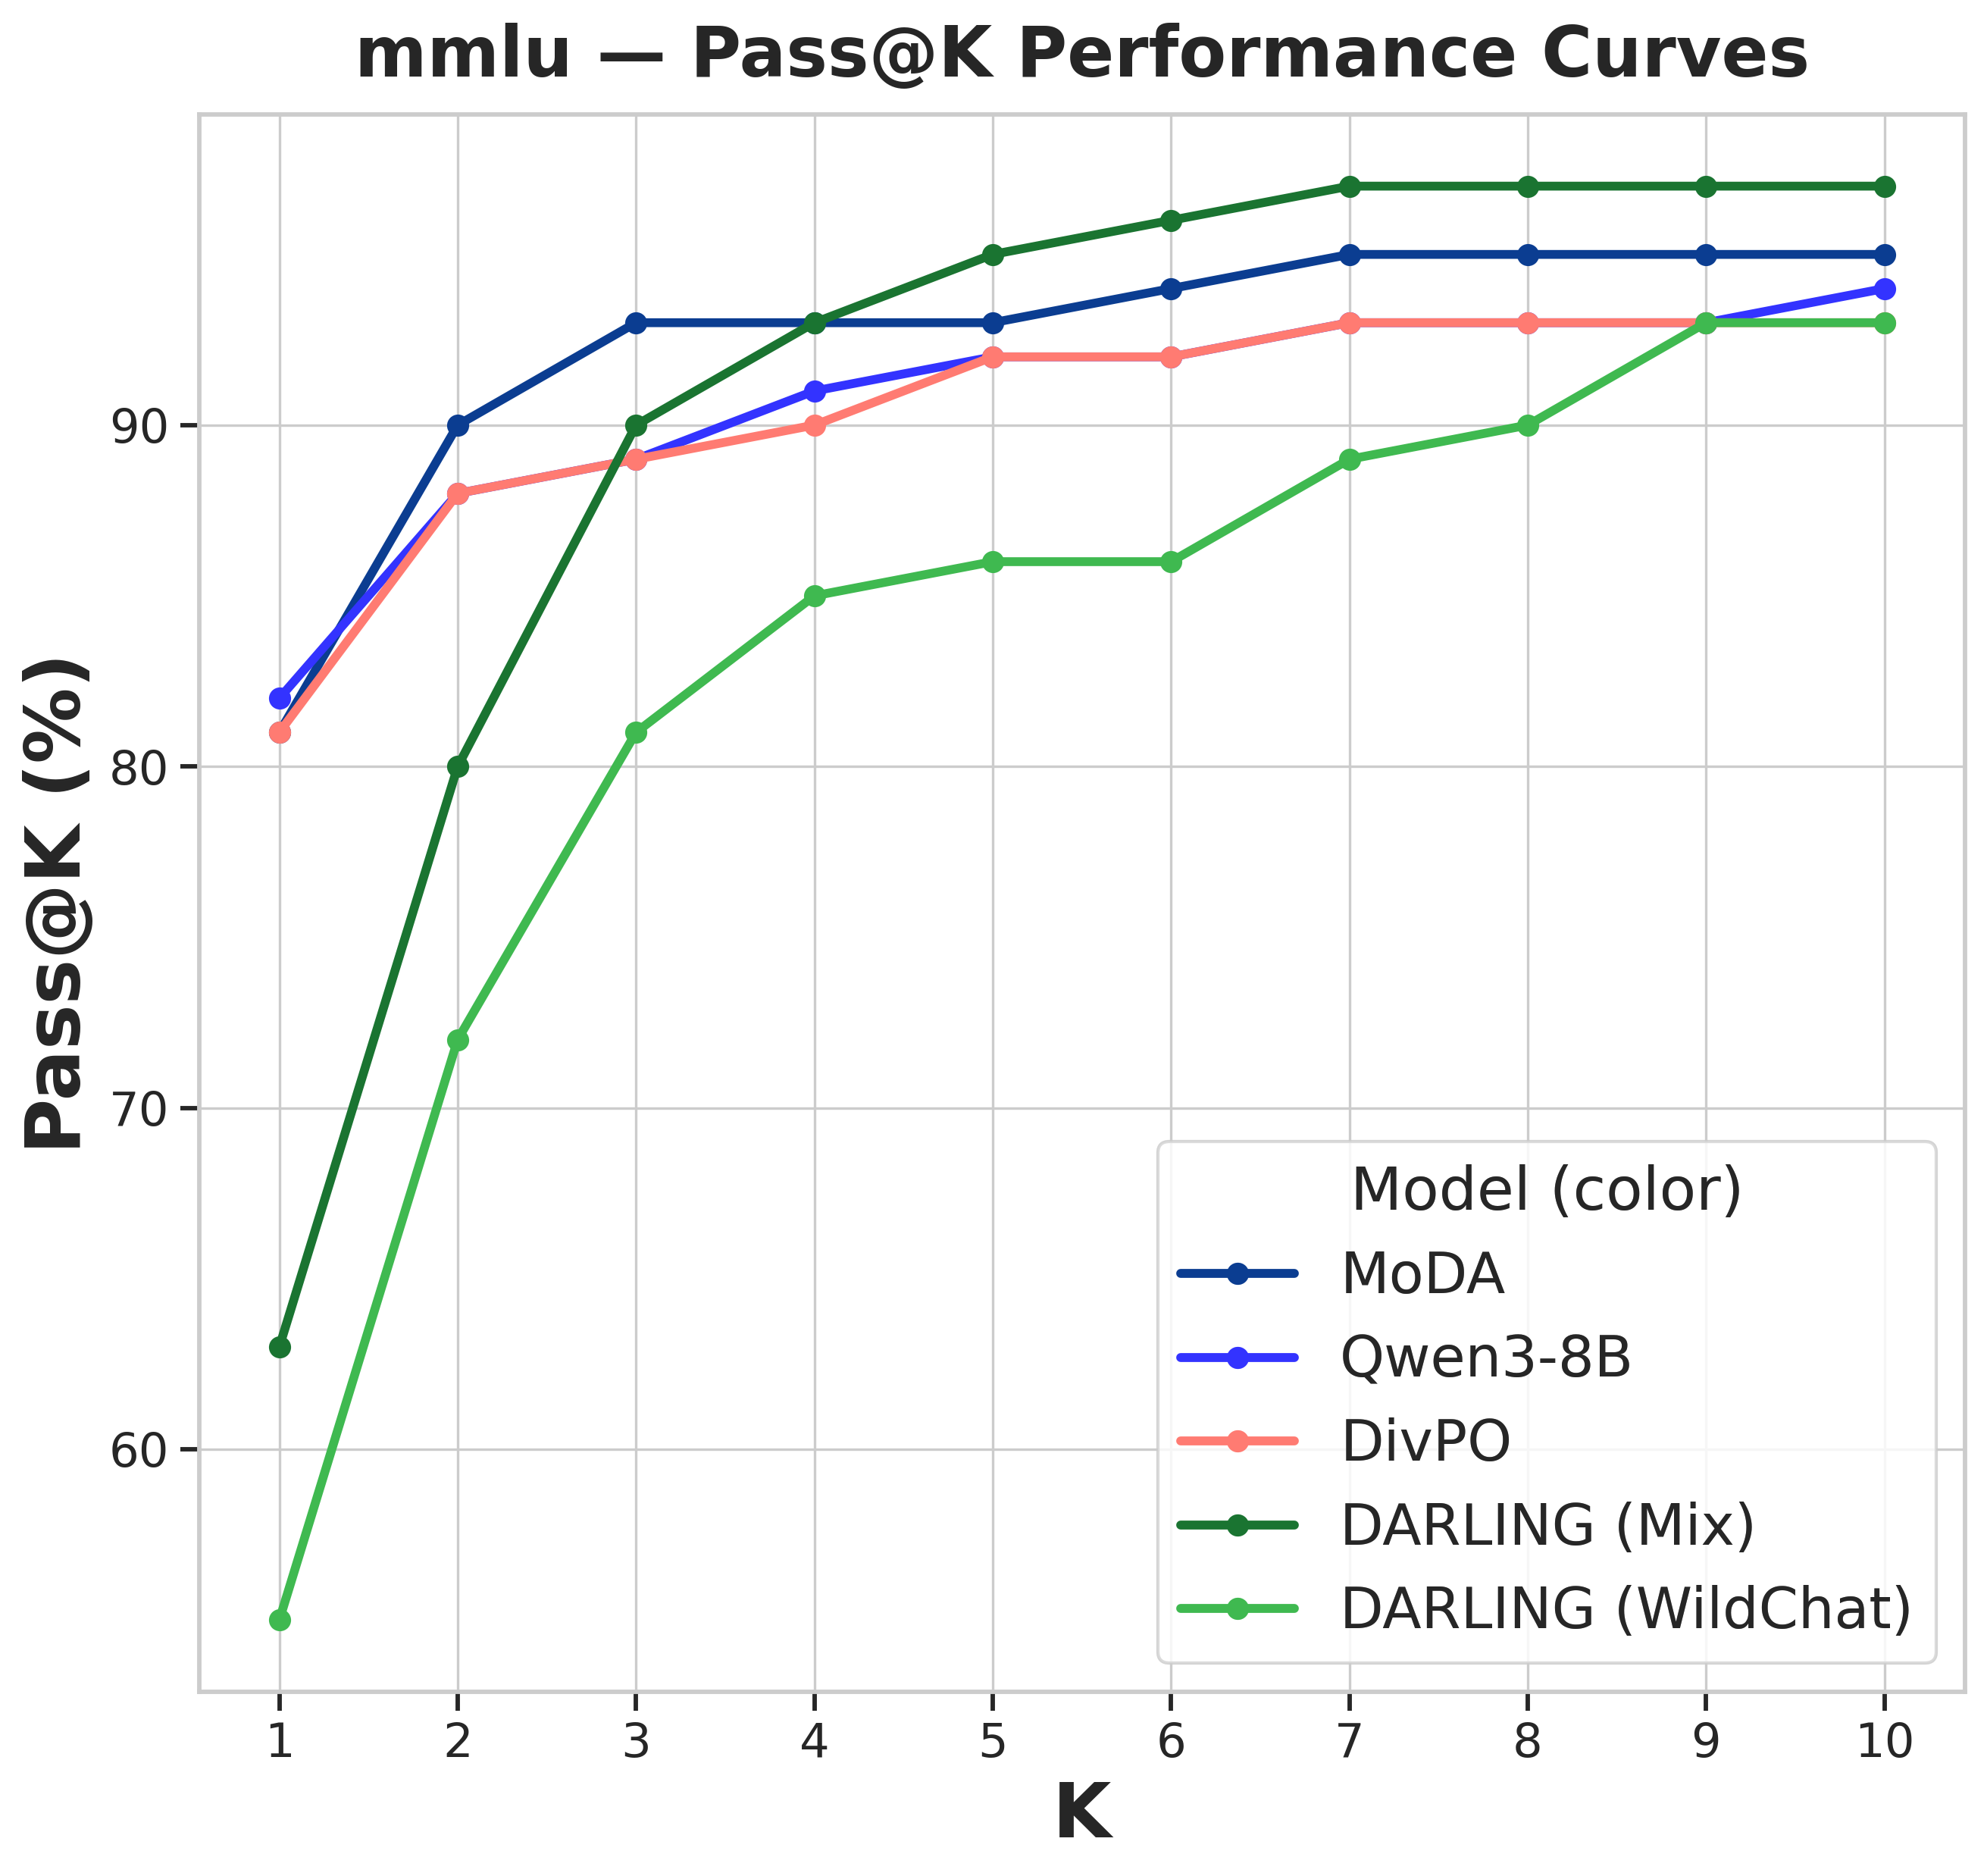
\includegraphics[width=\linewidth]{figures/main_pass_k/pass_at_k_figures/pass_at_k_mmlu_thinking_false_base_model_qwen3-8b.png}
\end{minipage}\hfill
\begin{minipage}{0.24\textwidth}
  \centering
  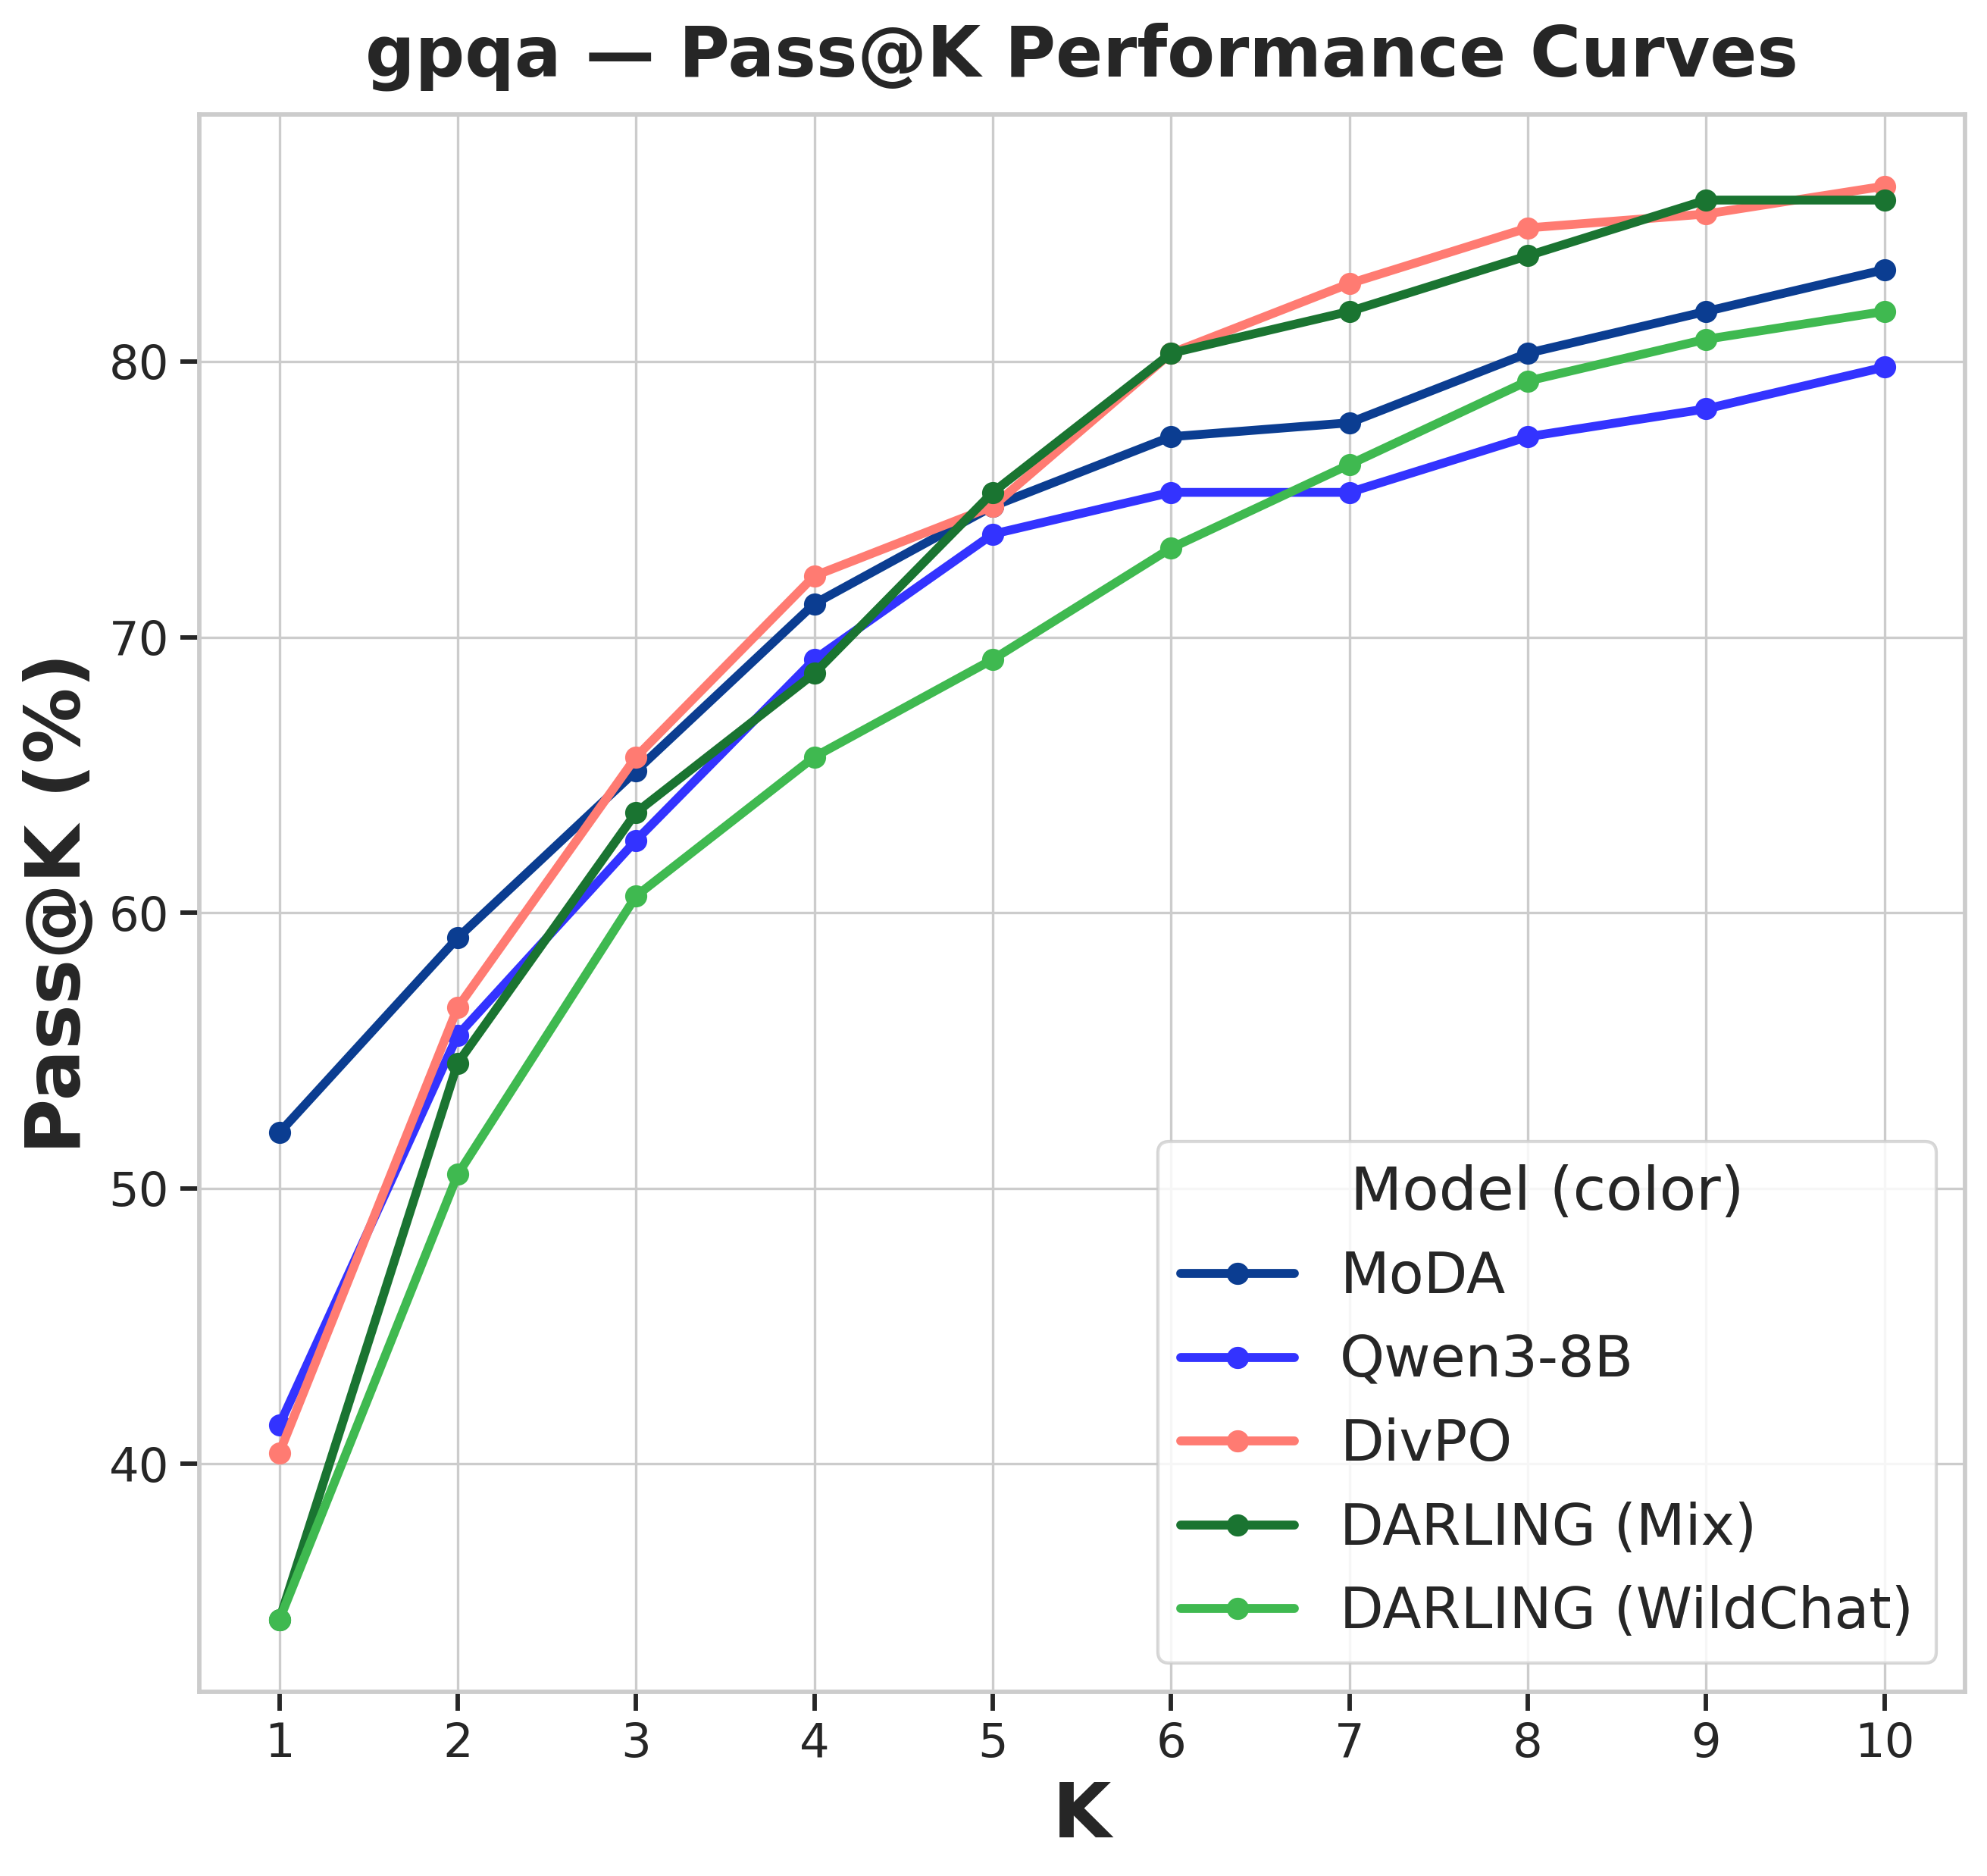
\includegraphics[width=\linewidth]{figures/main_pass_k/pass_at_k_figures/pass_at_k_gpqa_thinking_false_base_model_qwen3-8b.png}
\end{minipage}\hfill
\begin{minipage}{0.24\textwidth}
  \centering
  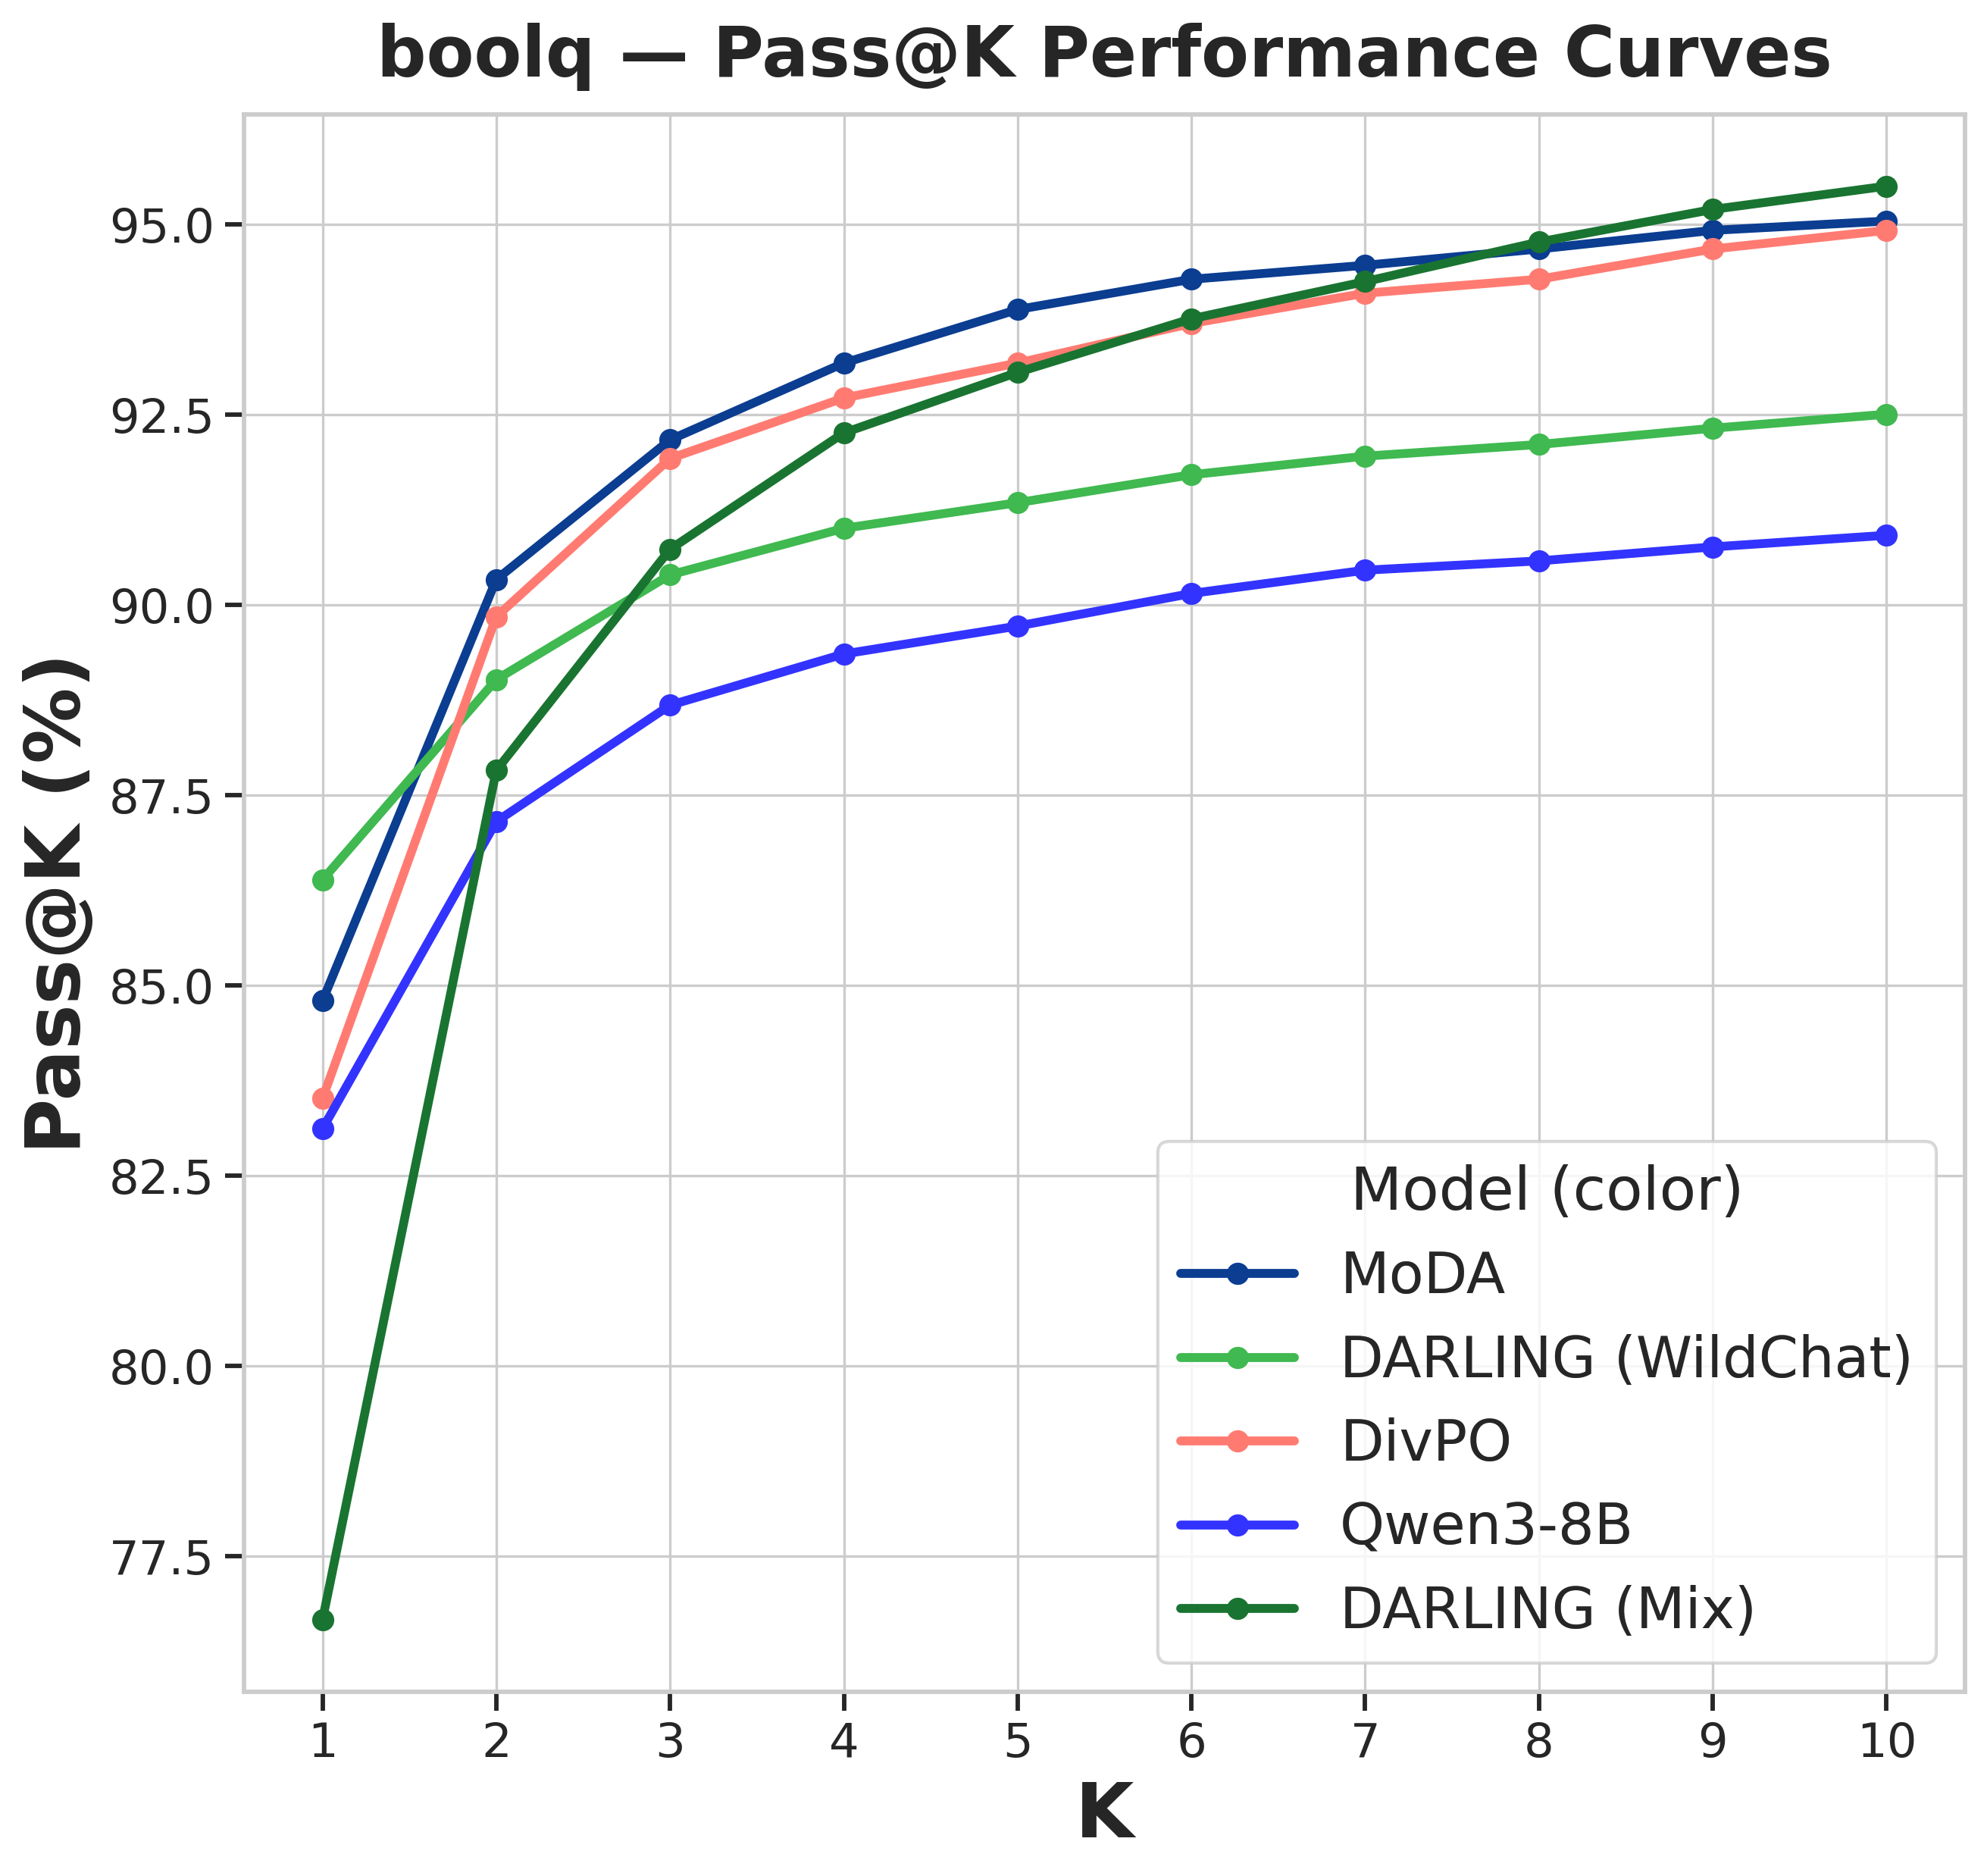
\includegraphics[width=\linewidth]{figures/main_pass_k/pass_at_k_figures/pass_at_k_boolq_thinking_false_base_model_qwen3-8b.png}
\end{minipage}

\vspace{4pt}
\begin{minipage}{0.24\textwidth}
  \centering
  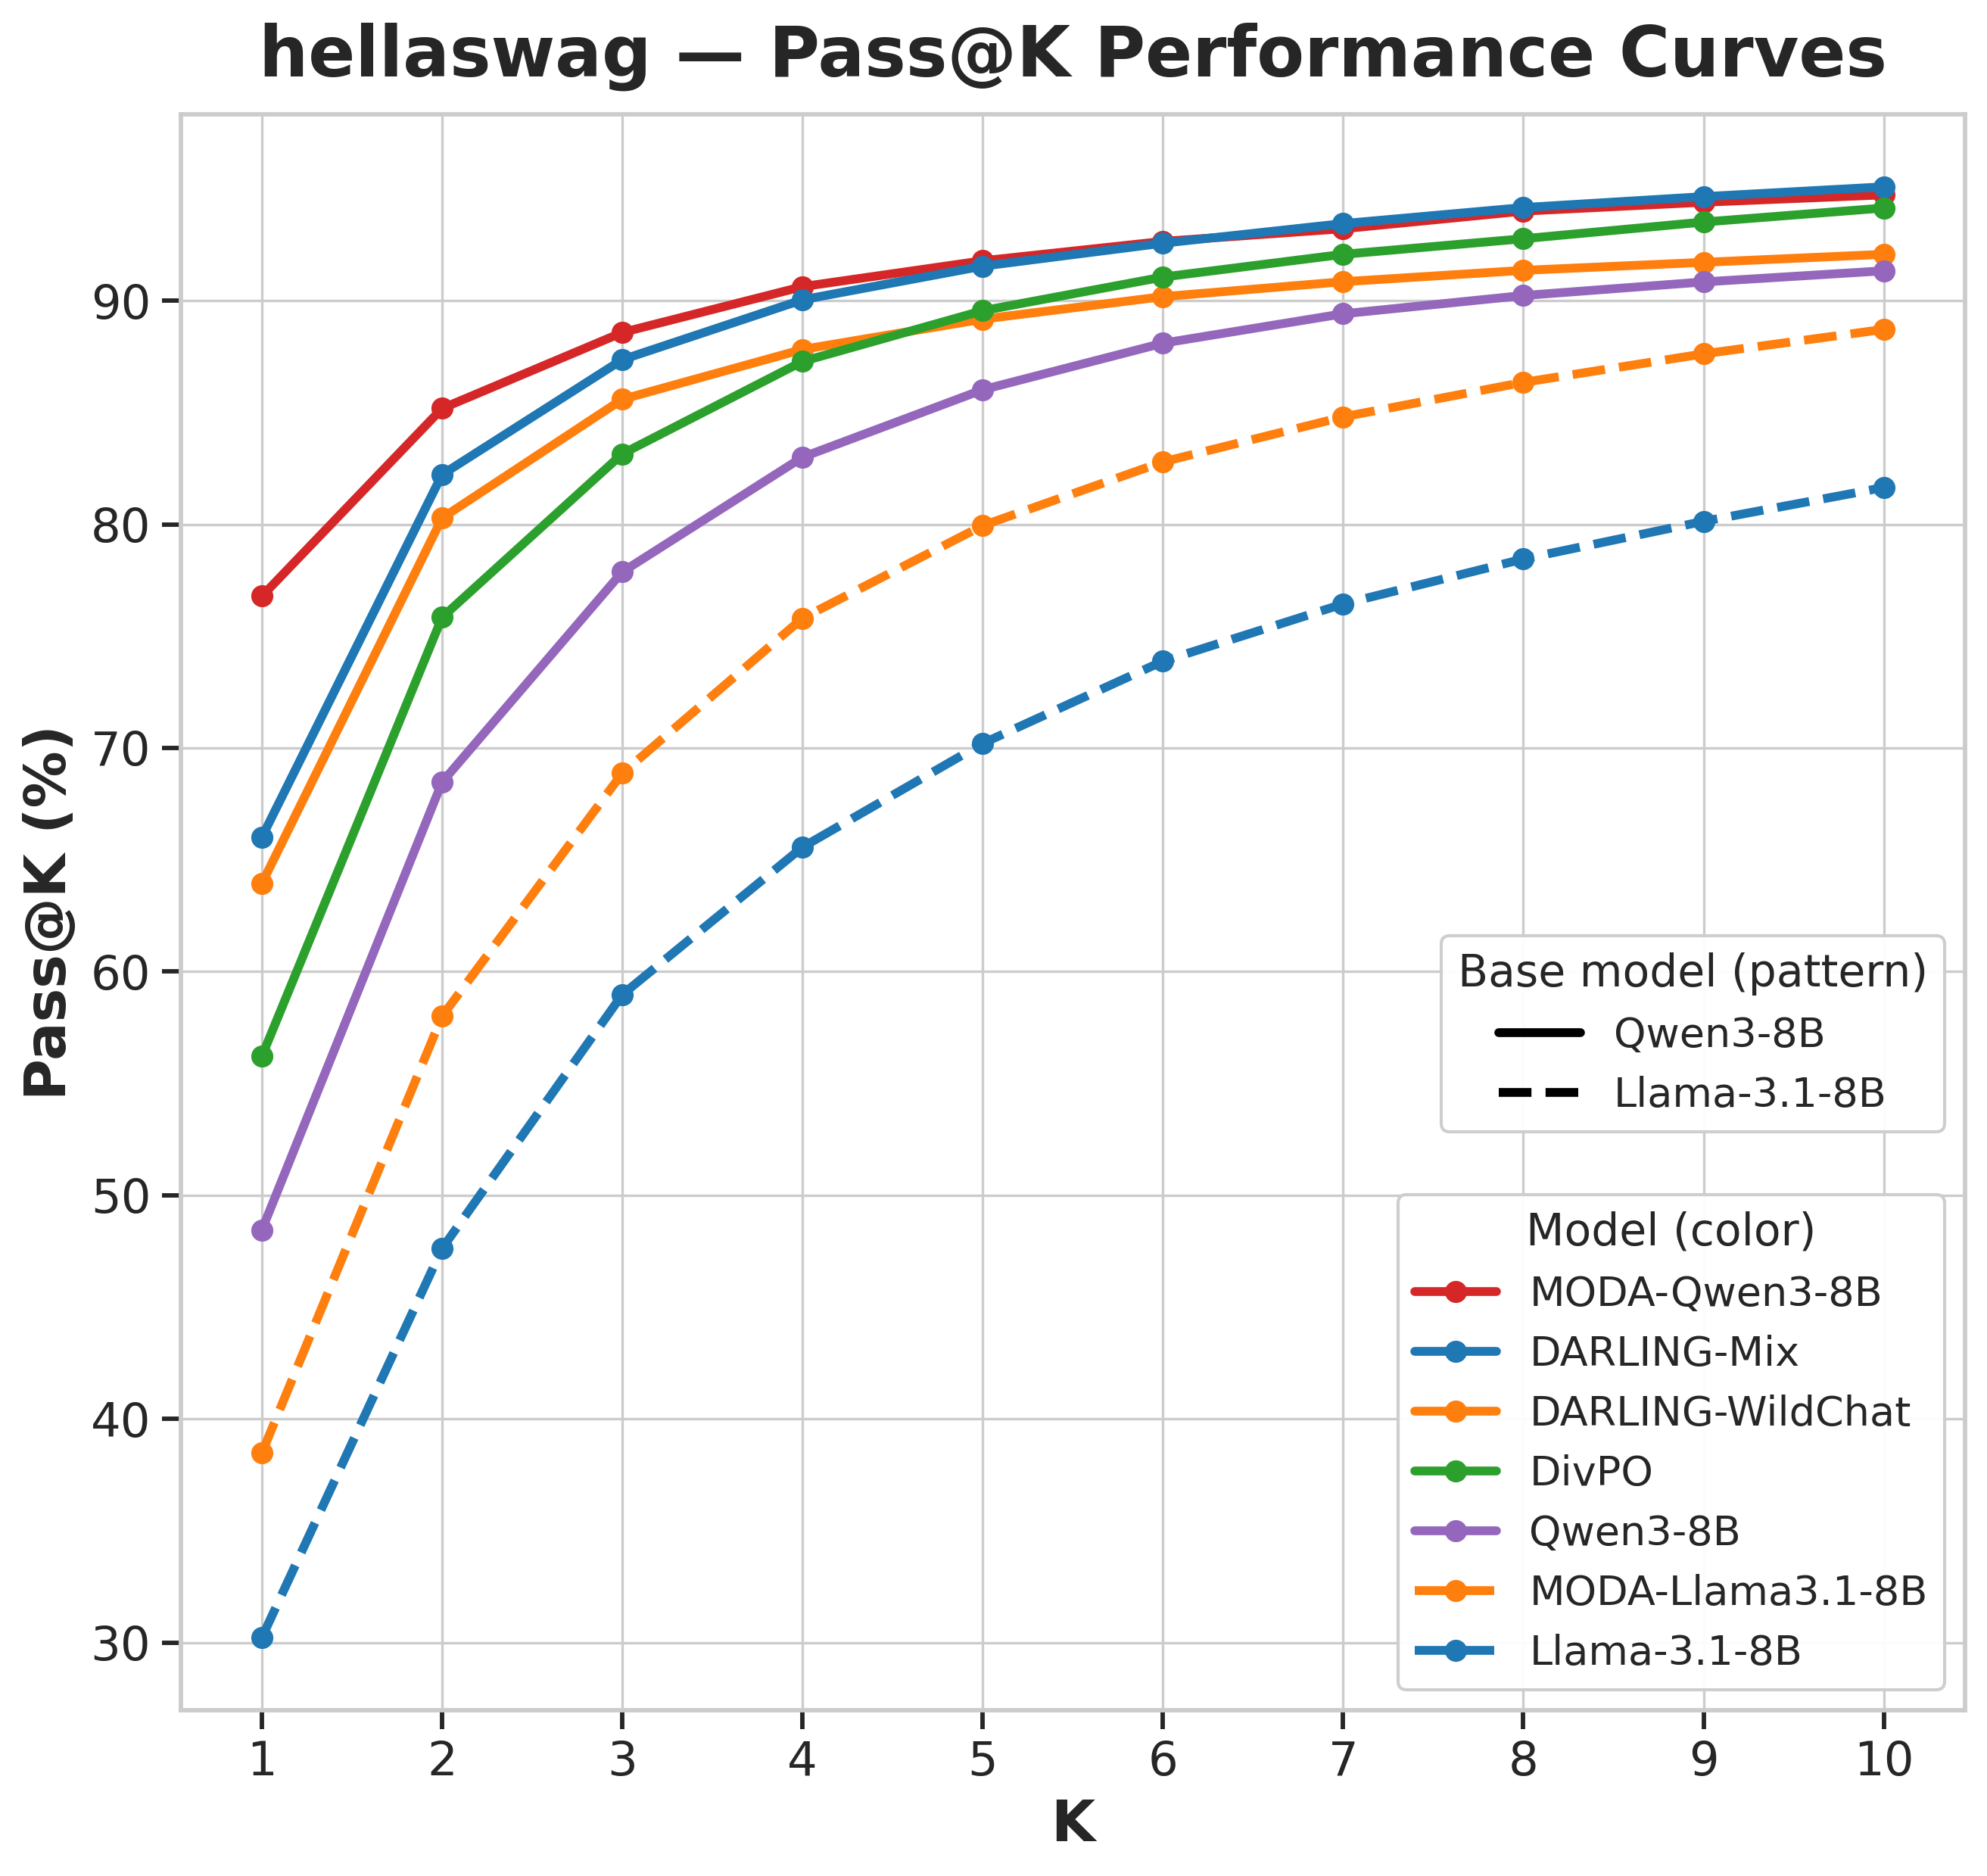
\includegraphics[width=\linewidth]{figures/main_pass_k/pass_at_k_curves_hellaswag.png}
\end{minipage}\hfill
\begin{minipage}{0.24\textwidth}
  \centering
  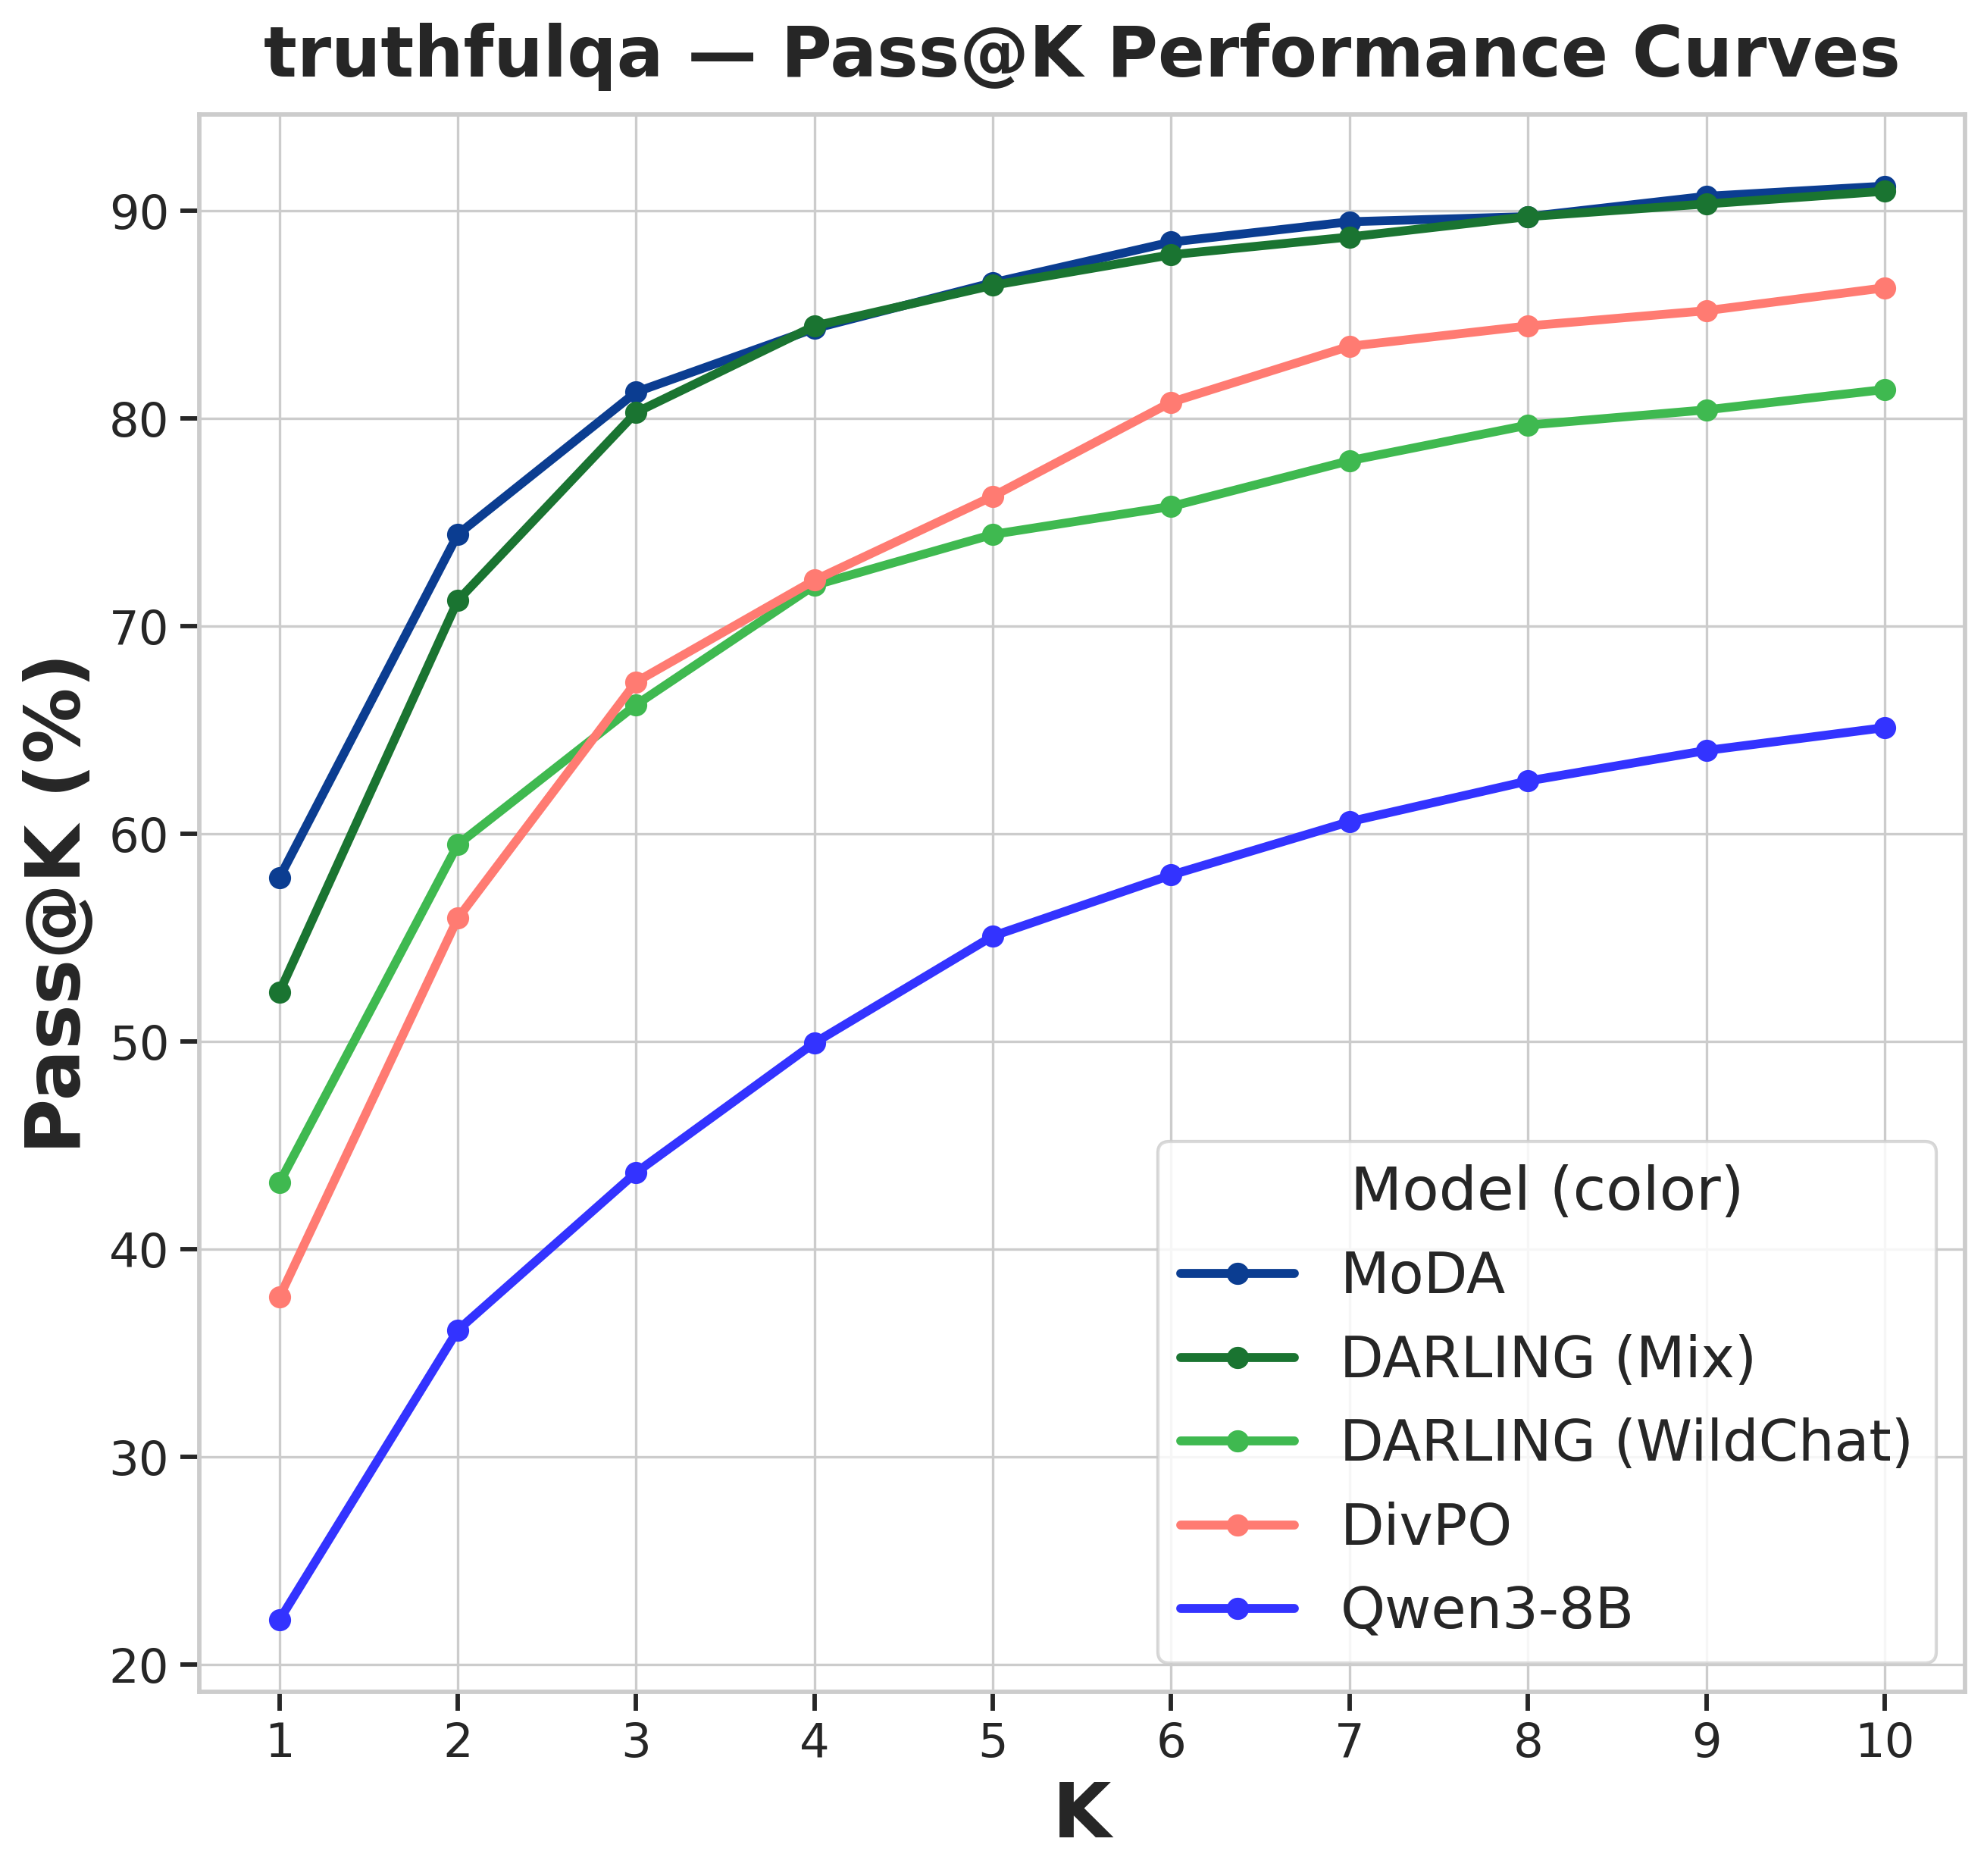
\includegraphics[width=\linewidth]{figures/main_pass_k/pass_at_k_figures/pass_at_k_truthfulqa_thinking_false_base_model_qwen3-8b.png}
\end{minipage}\hfill
\begin{minipage}{0.24\textwidth}
  \centering
  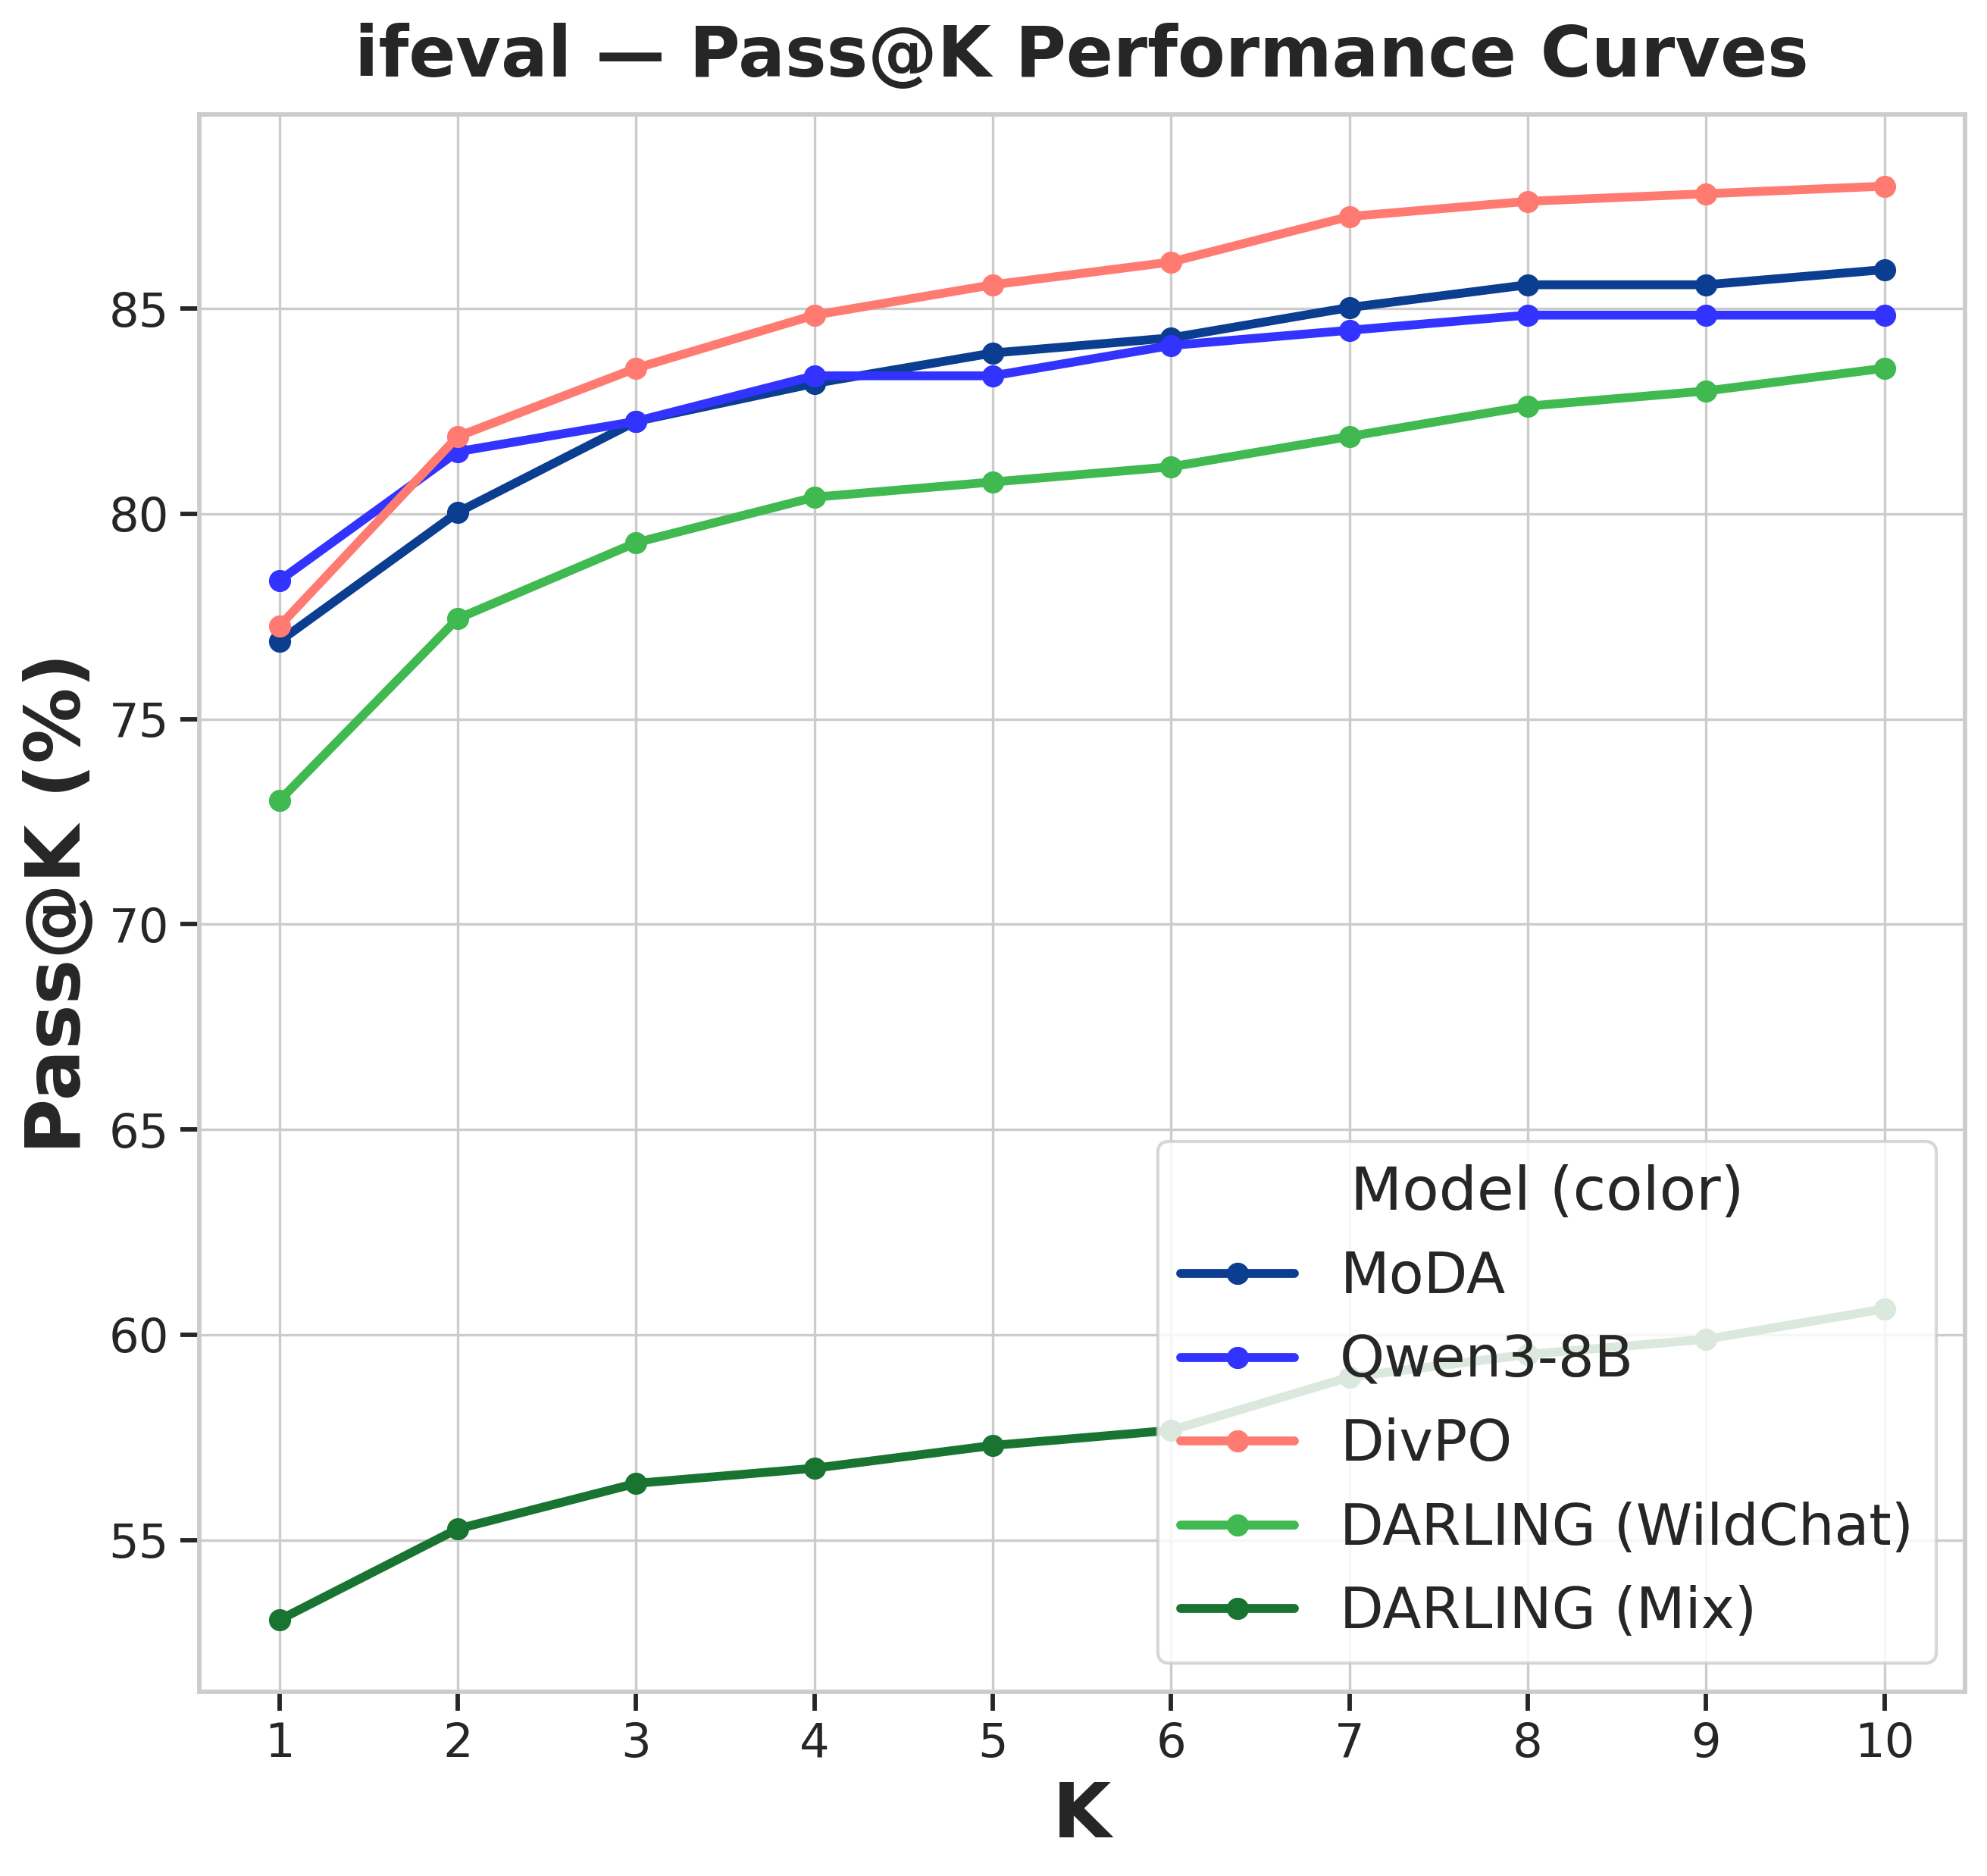
\includegraphics[width=\linewidth]{figures/main_pass_k/pass_at_k_figures/pass_at_k_ifeval_thinking_false_base_model_qwen3-8b.png}
\end{minipage}
\caption{\textbf{General capability retention: pass@k accuracy.} Qwen3-8B base and thinking disabled models on the general capability suite tasks: GSM8K, MMLU, GPQA, BoolQ, HellaSwag, TruthfulQA, and IFEval. The suite average is shown in Figure~\ref{fig:general capability pass@k} in the main text.}
\label{fig:general capability pass@k thinking disabled}
\end{figure}


\begin{figure}[H]
\begin{minipage}{0.24\textwidth}
  \centering
  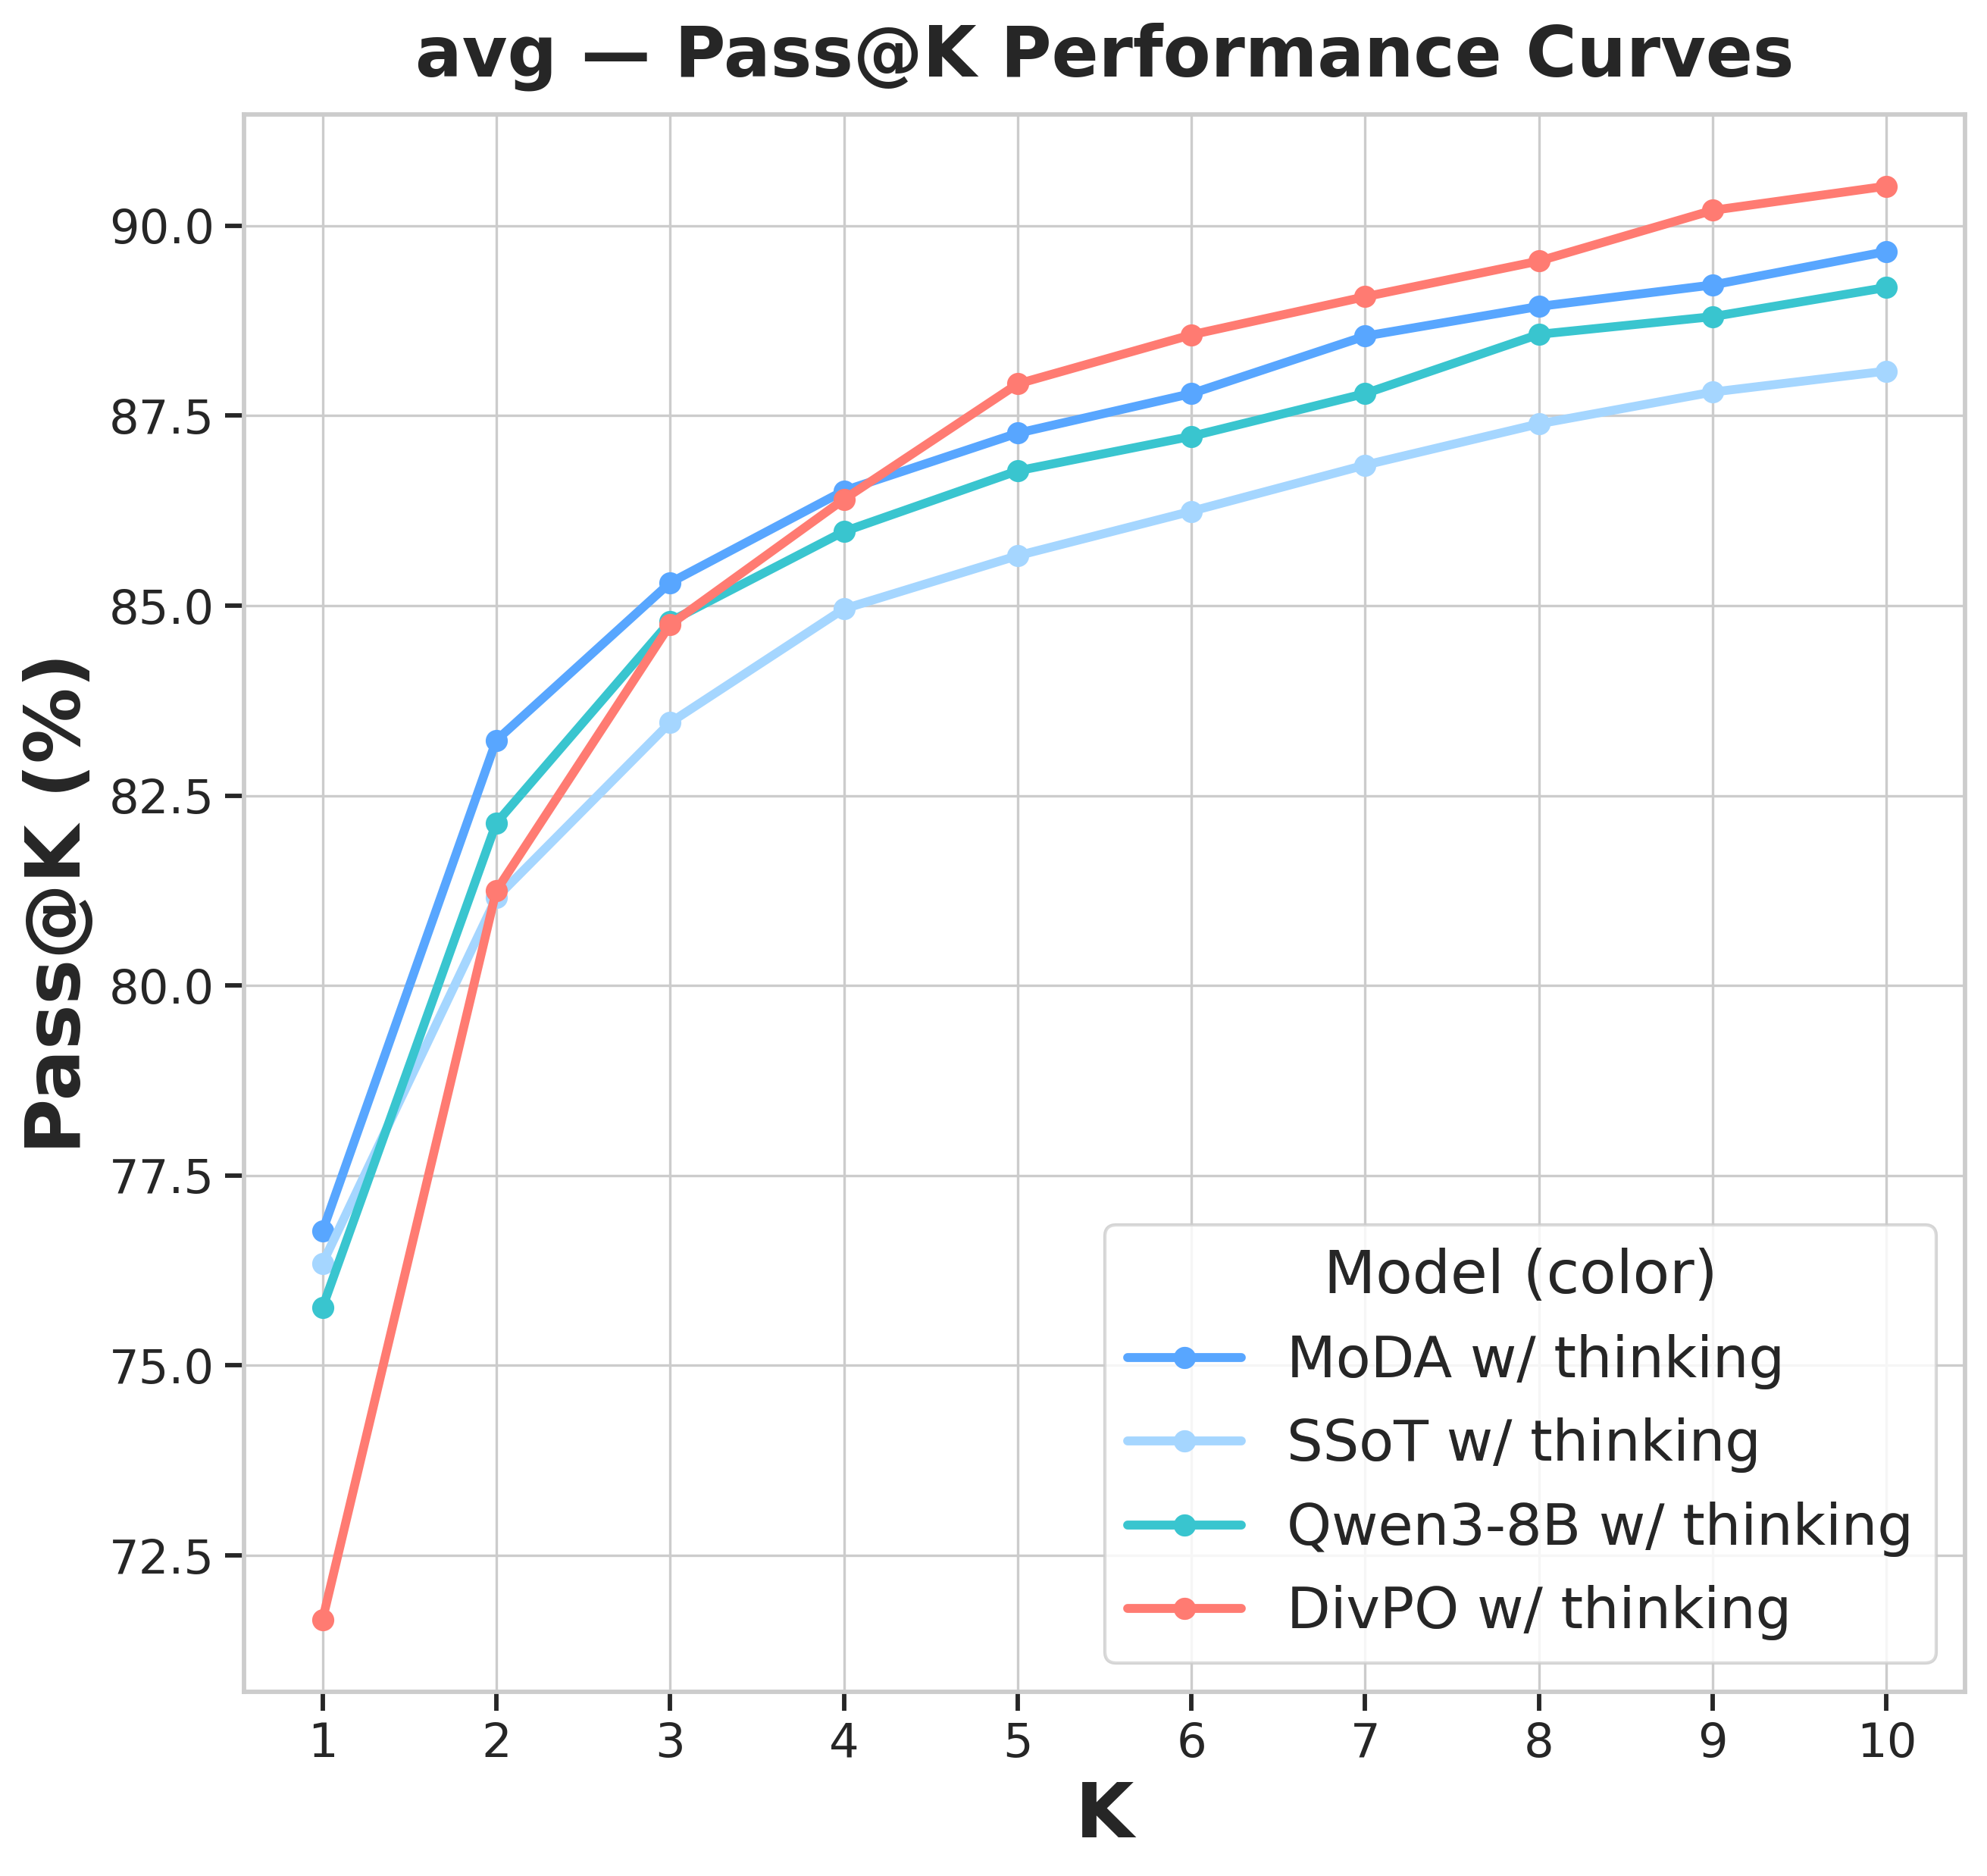
\includegraphics[width=\linewidth]{figures/main_pass_k/pass_at_k_figures/pass_at_k_avg_thinking_true.png}
\end{minipage}\hfill
\centering
\begin{minipage}{0.24\textwidth}
  \centering
  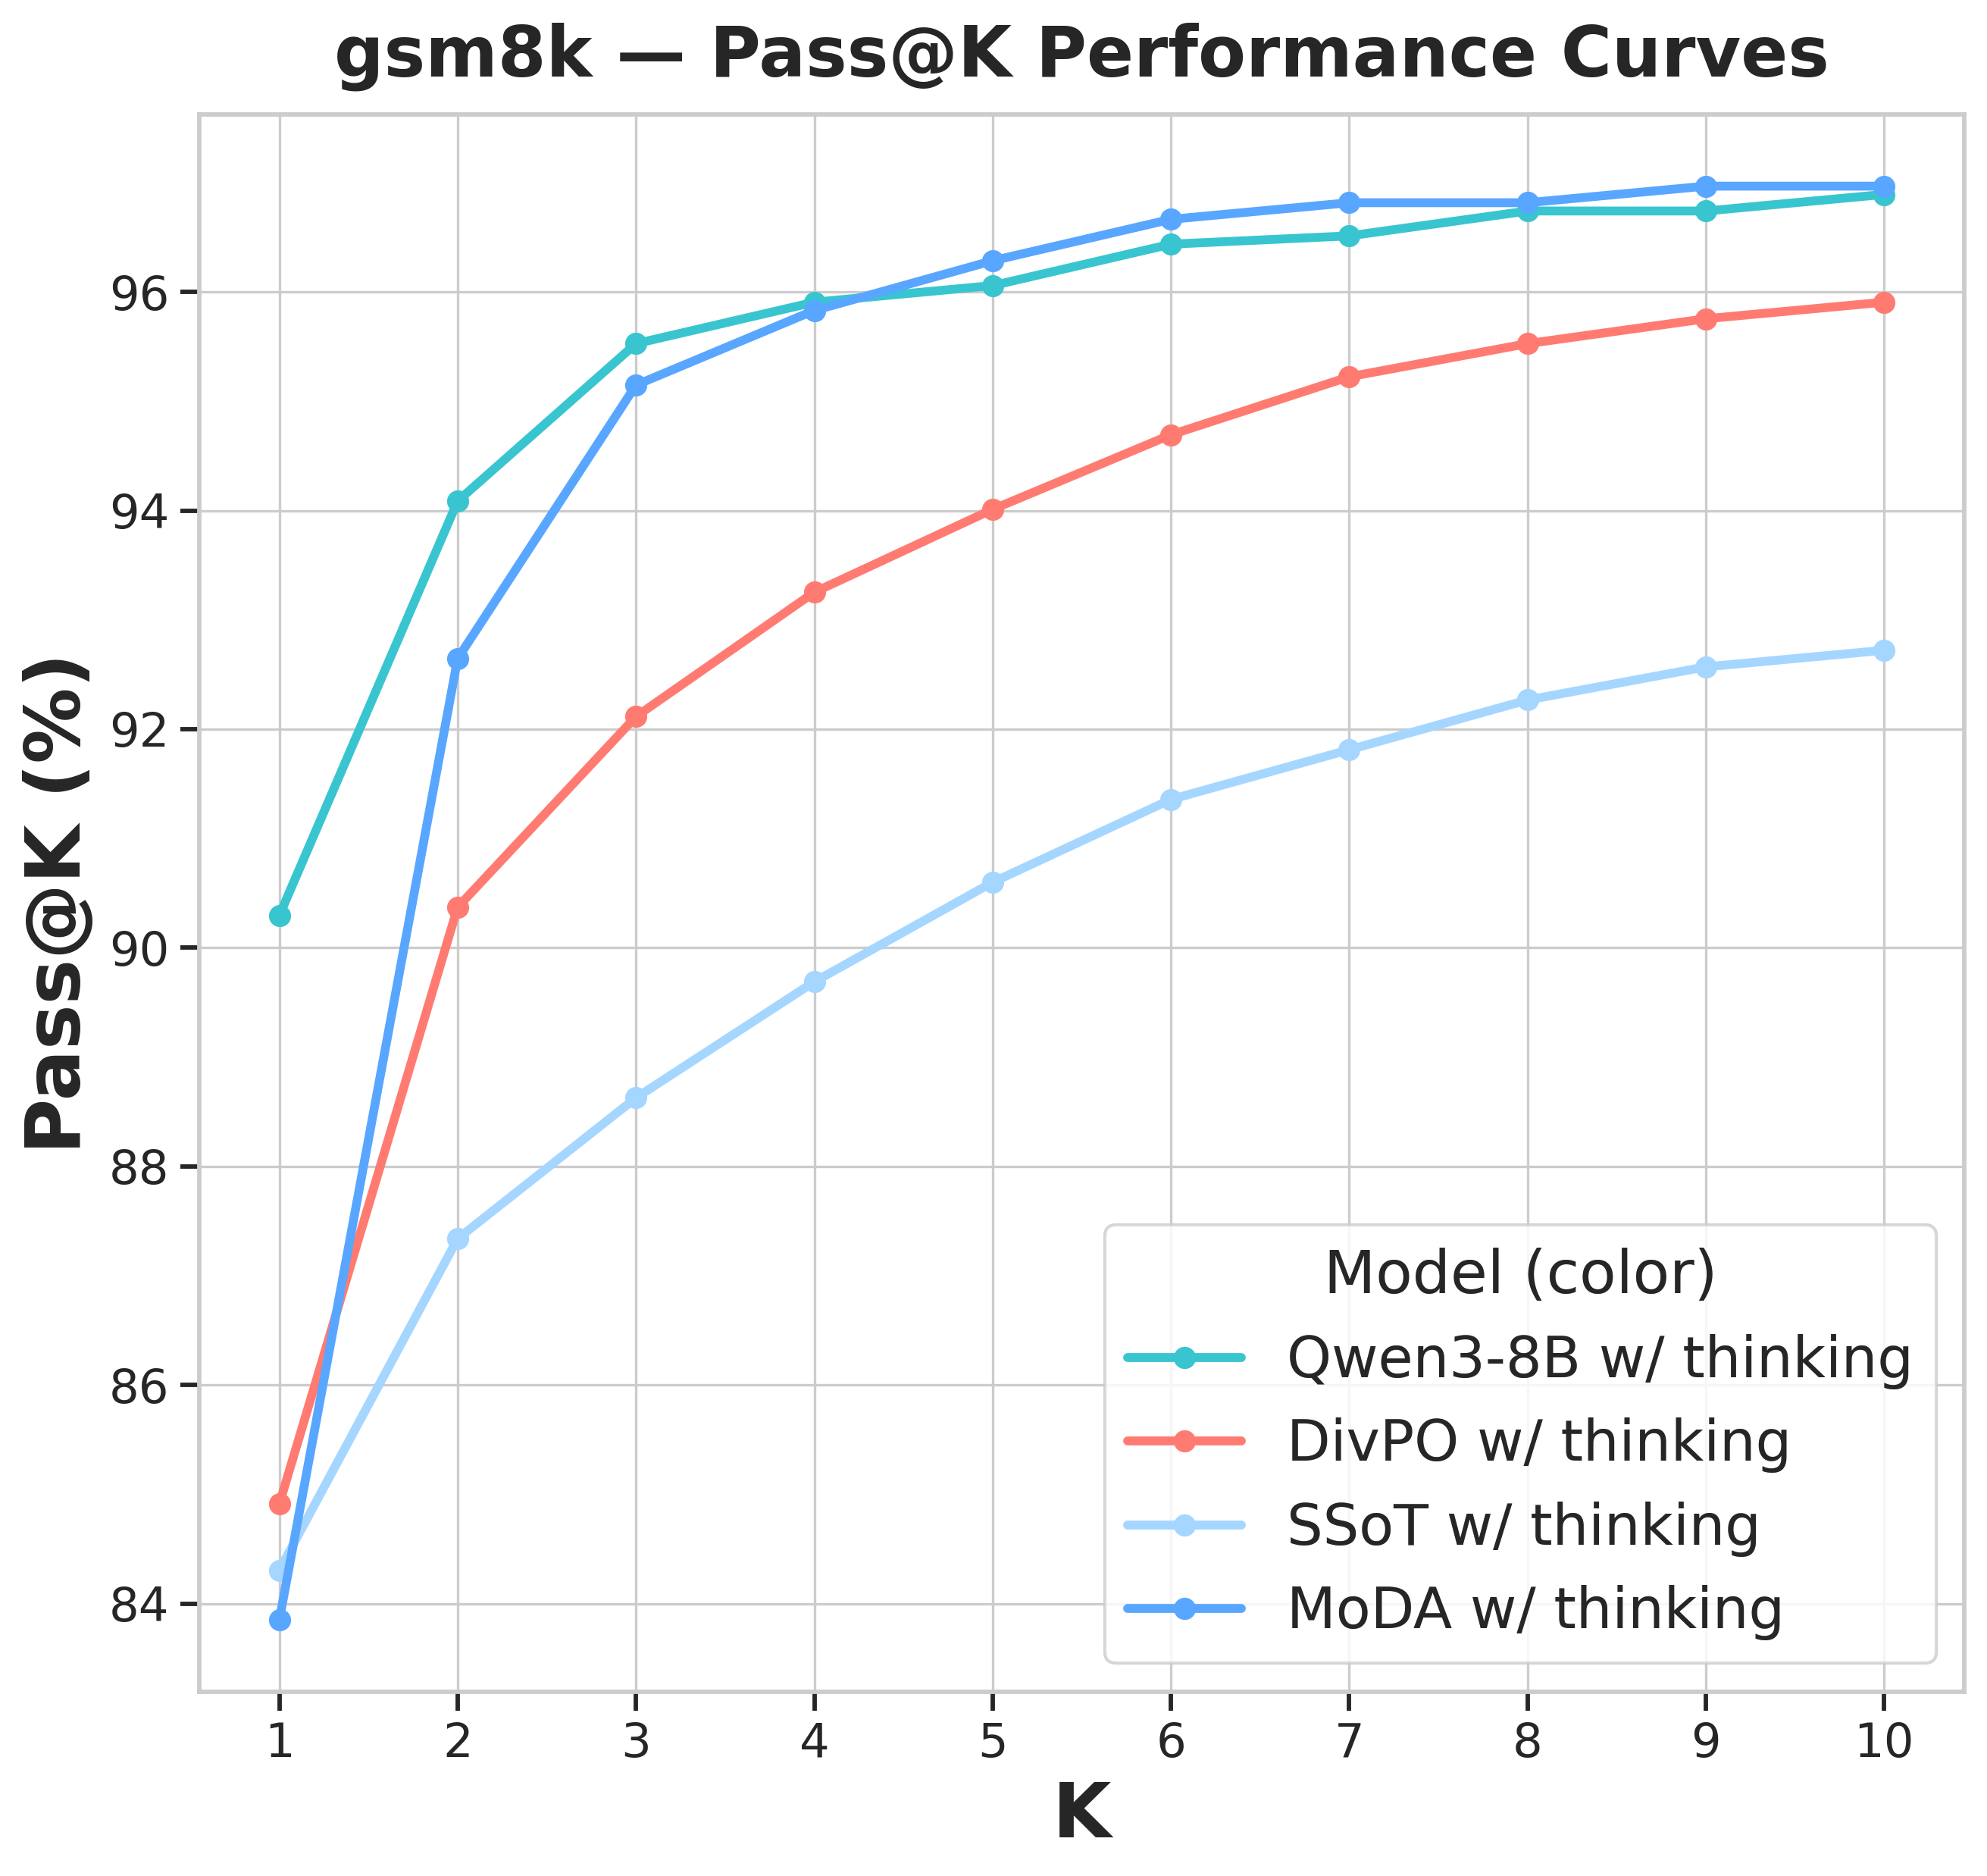
\includegraphics[width=\linewidth]{figures/main_pass_k/pass_at_k_figures/pass_at_k_gsm8k_thinking_true.png}
\end{minipage}\hfill
\begin{minipage}{0.24\textwidth}
  \centering
  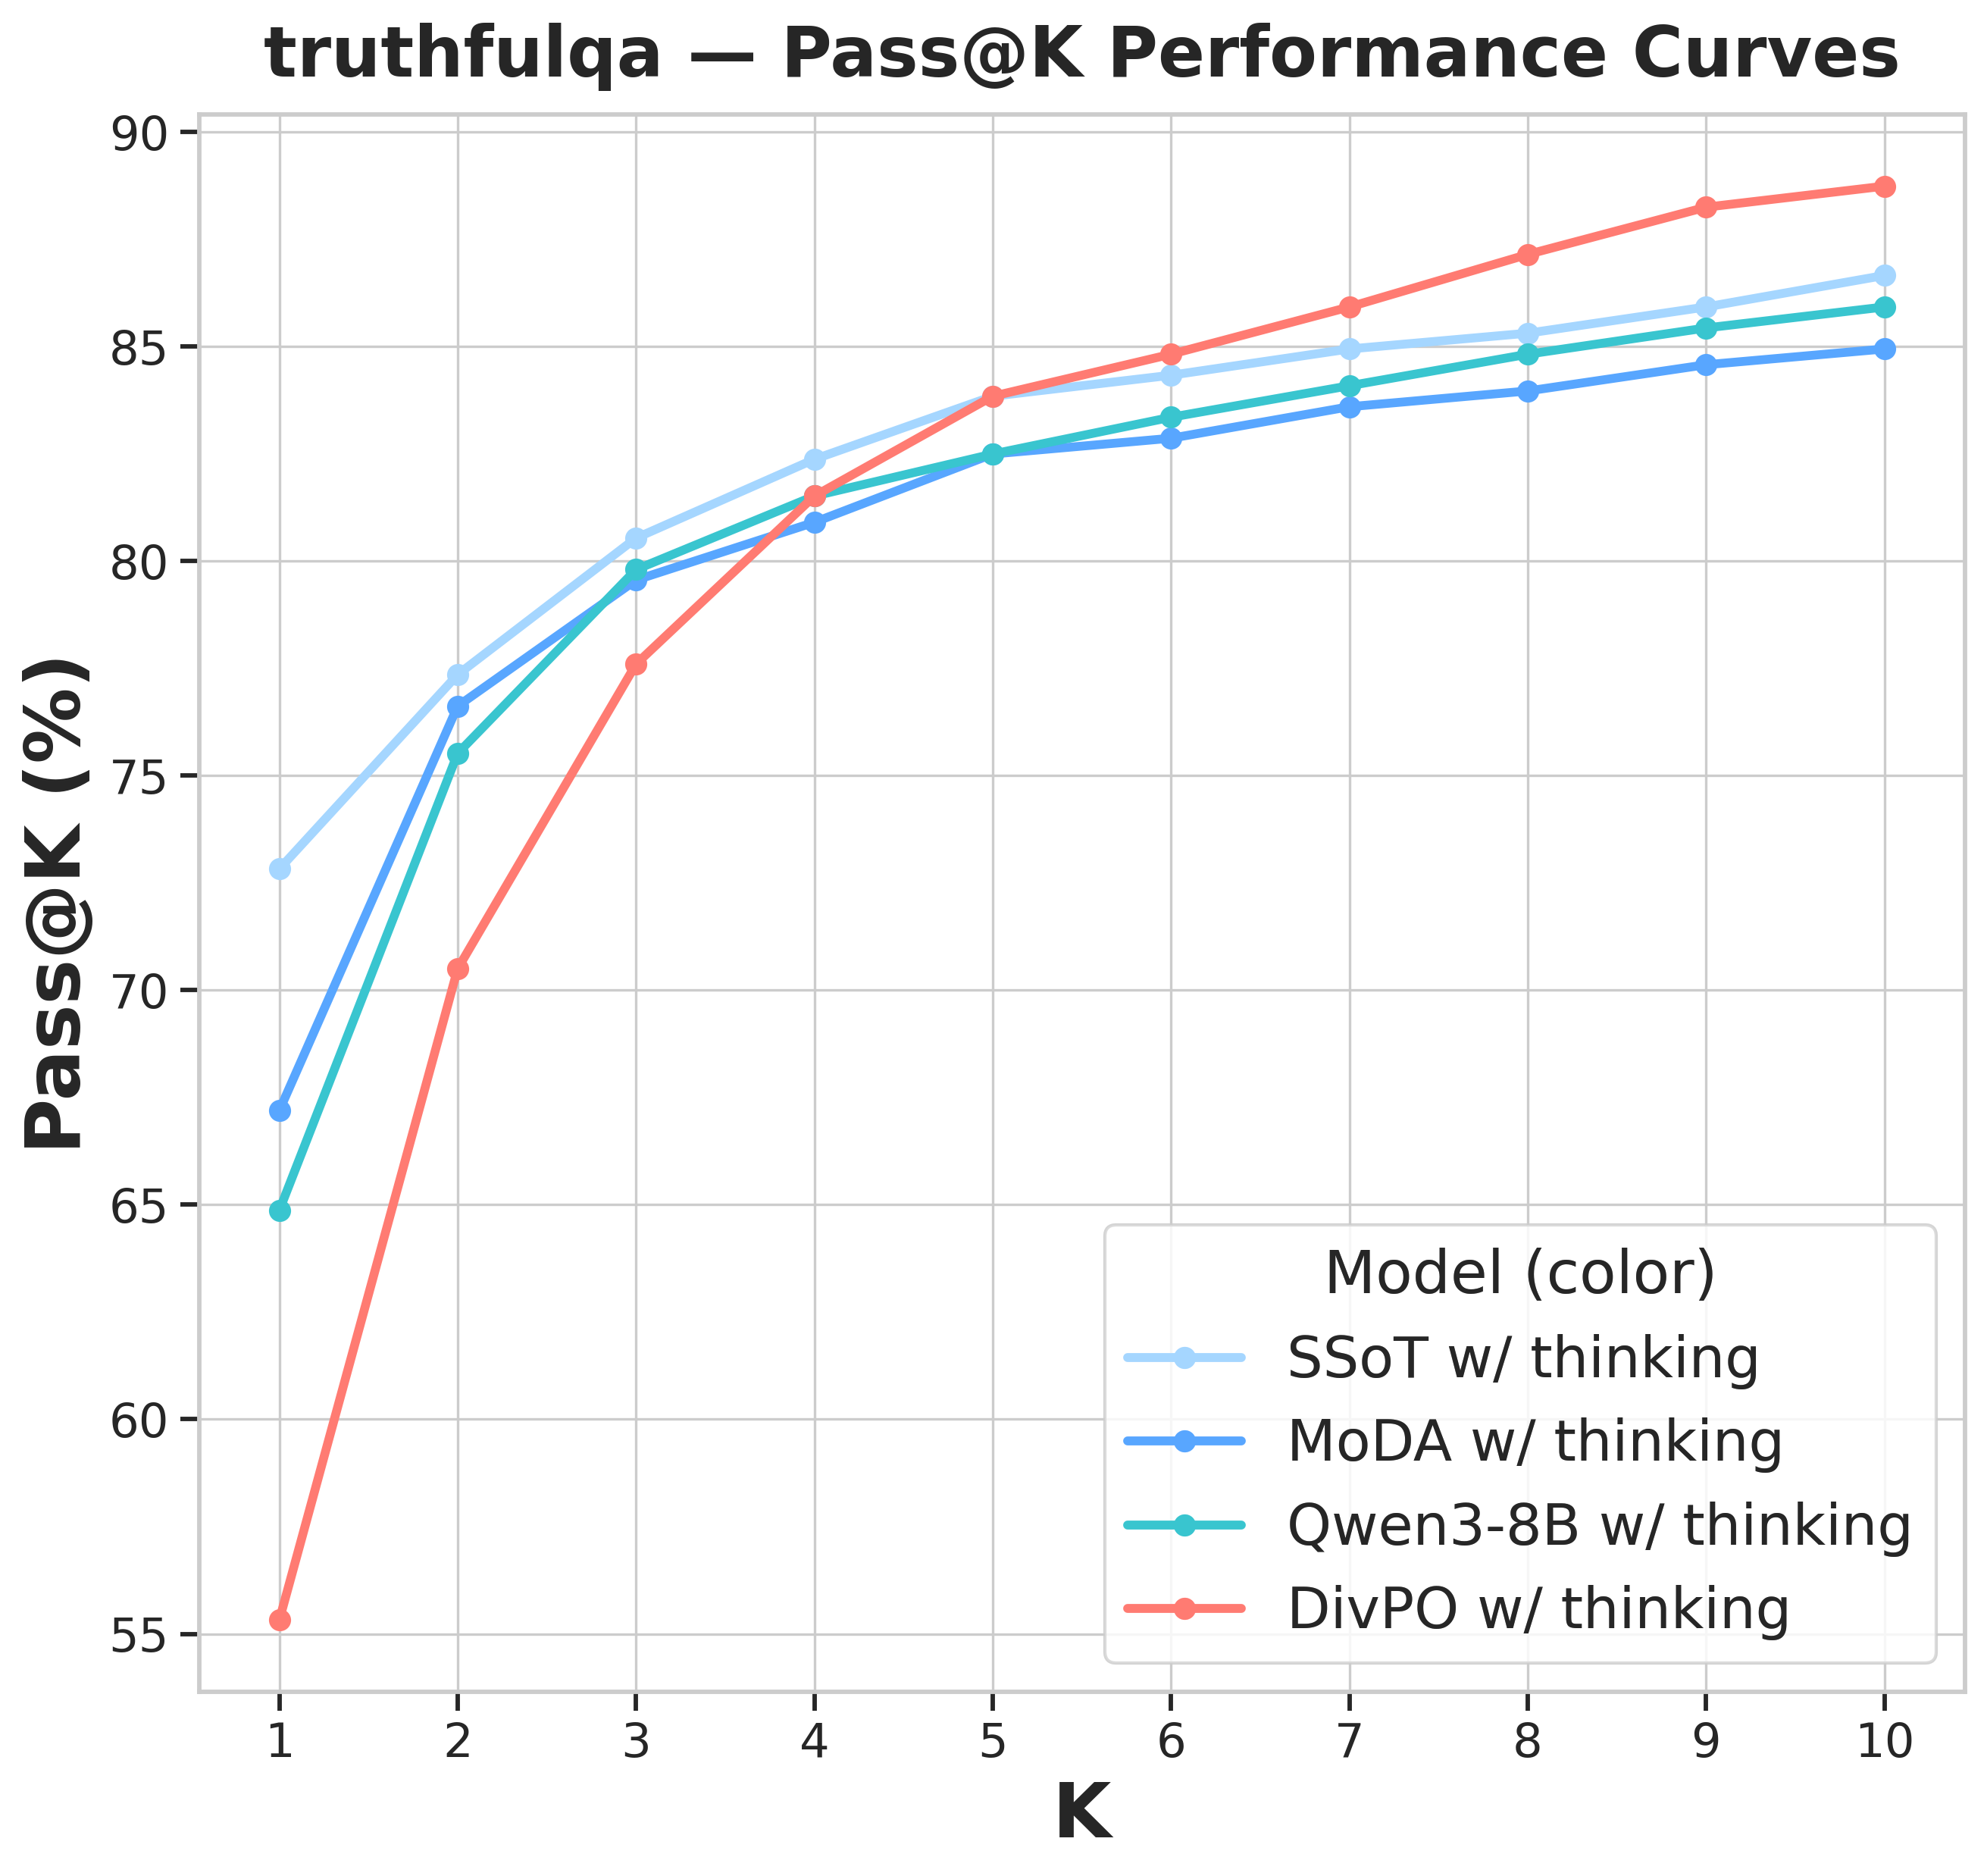
\includegraphics[width=\linewidth]{figures/main_pass_k/pass_at_k_figures/pass_at_k_truthfulqa_thinking_true.png}
\end{minipage}\hfill
\begin{minipage}{0.24\textwidth}
  \centering
  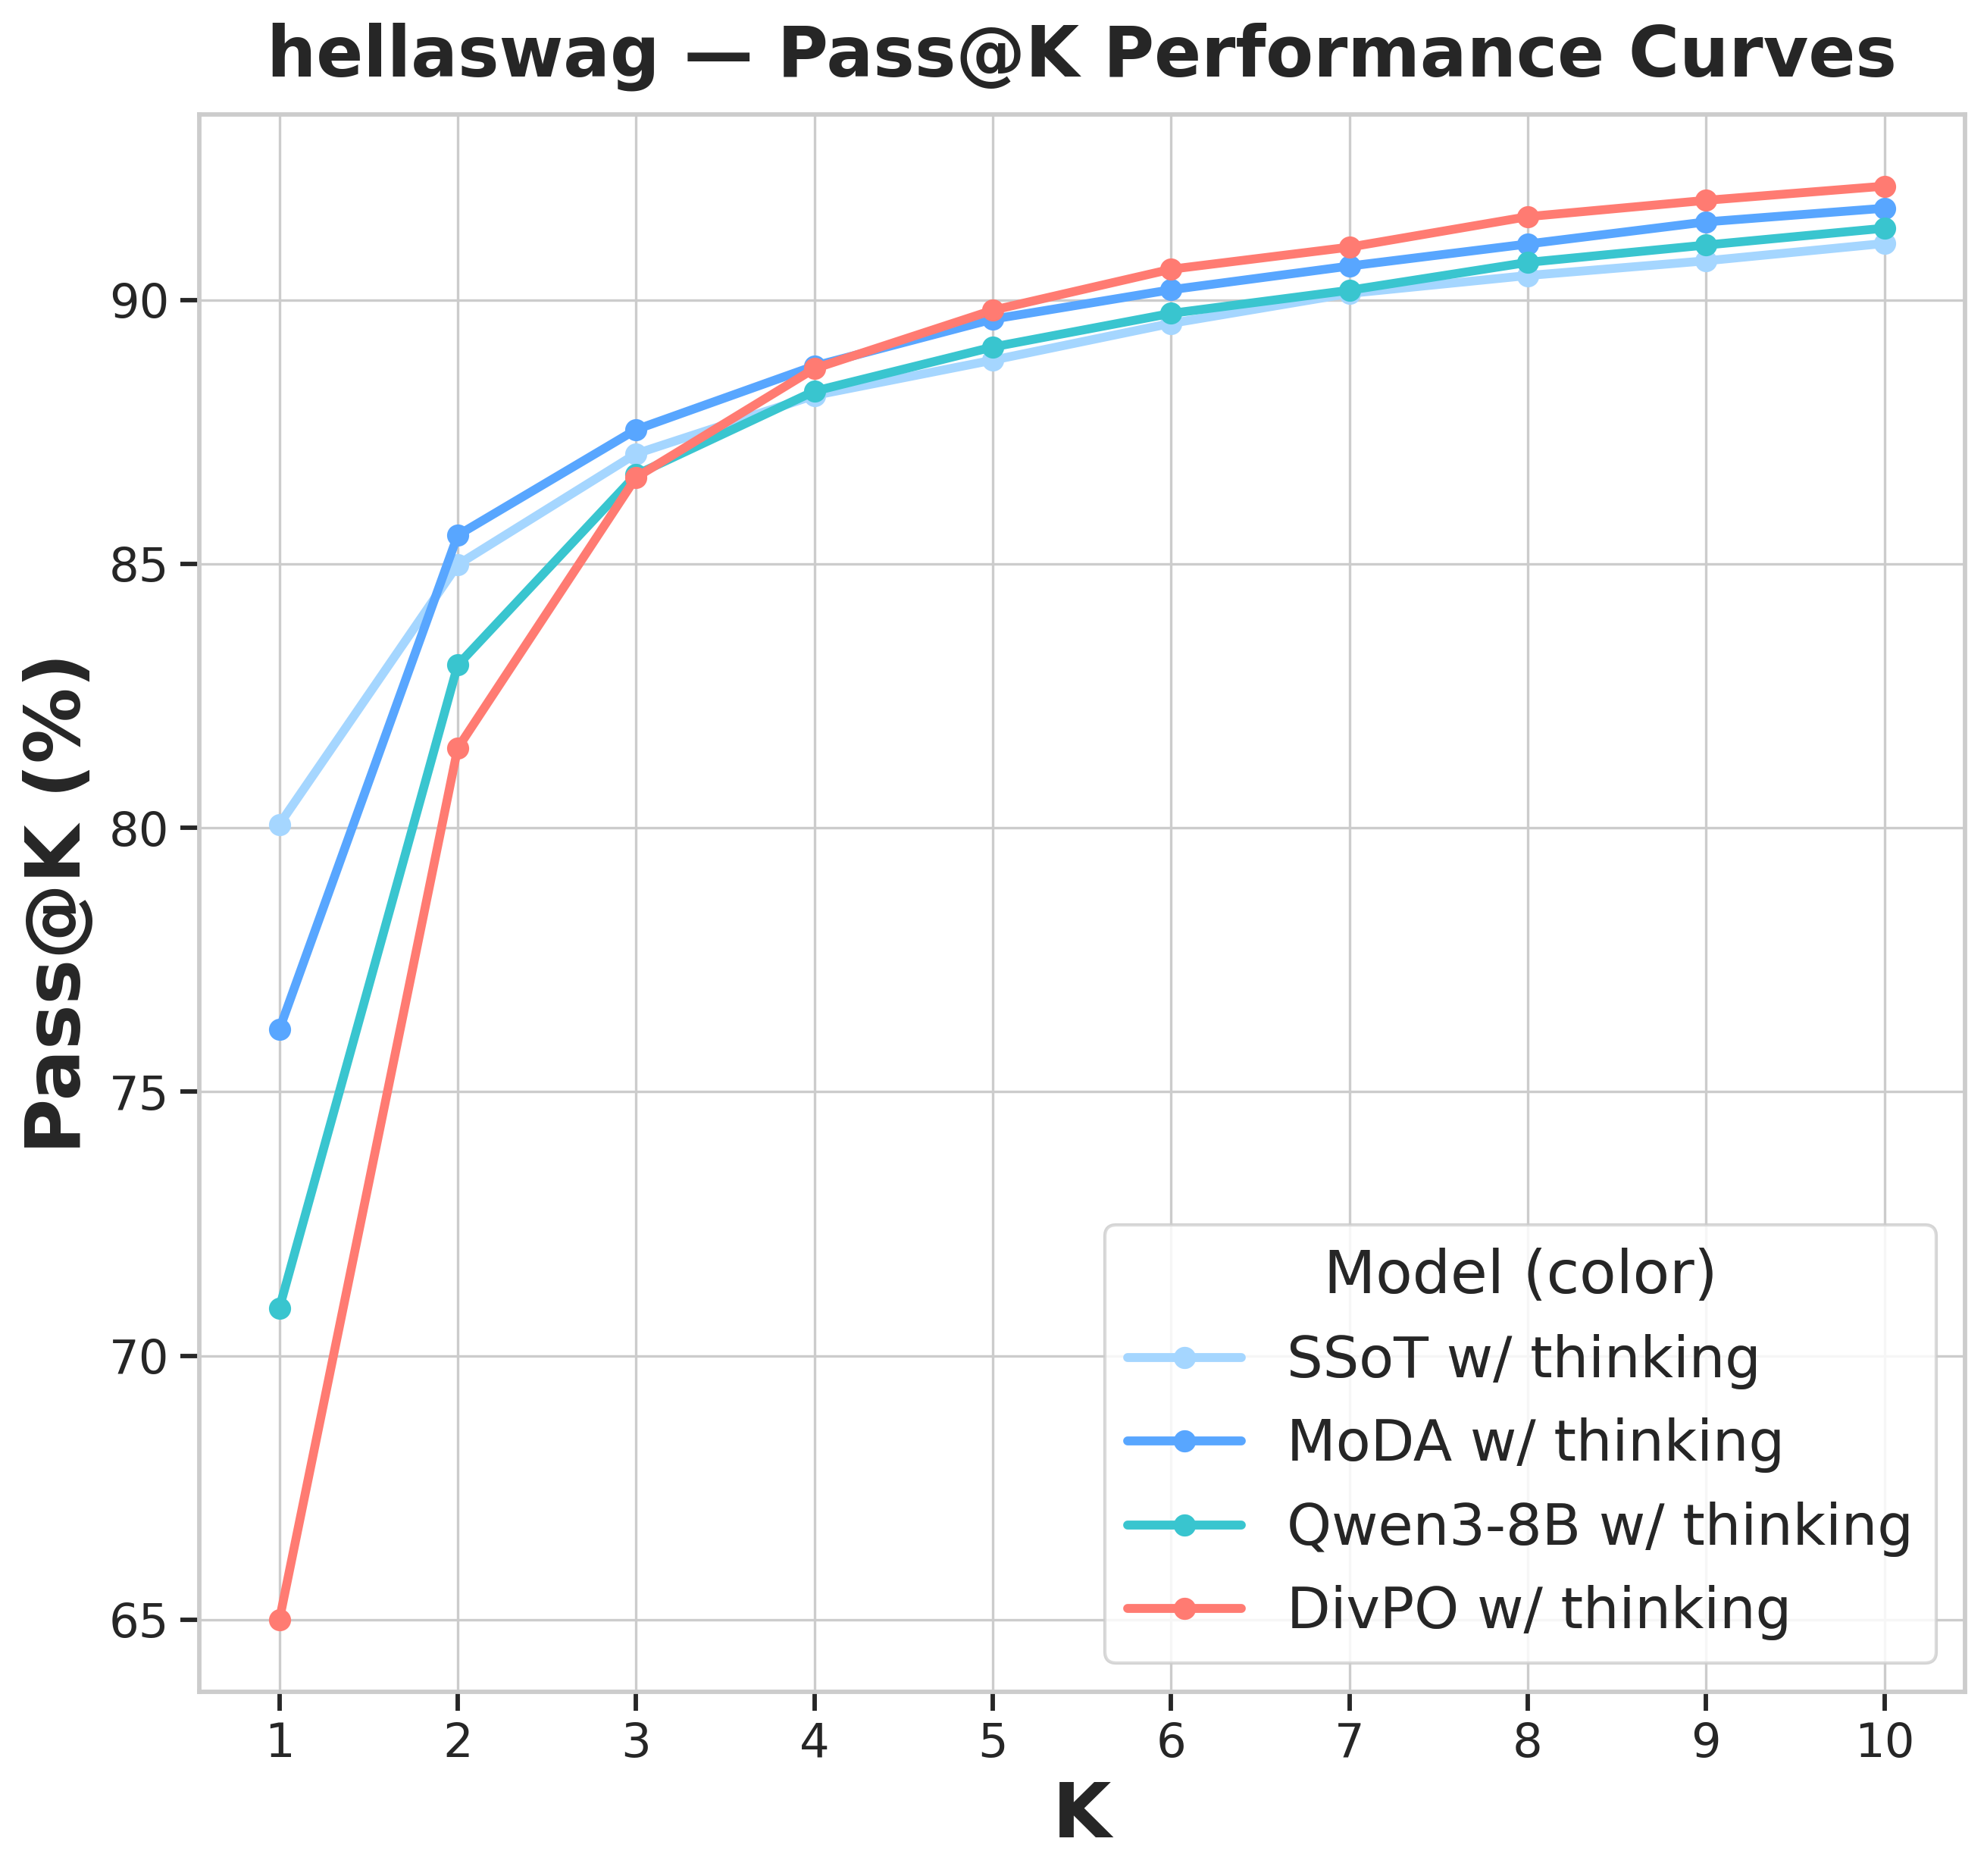
\includegraphics[width=\linewidth]{figures/main_pass_k/pass_at_k_figures/pass_at_k_hellaswag_thinking_true.png}
\end{minipage}
\centering
\begin{minipage}{0.24\textwidth}
  \centering
  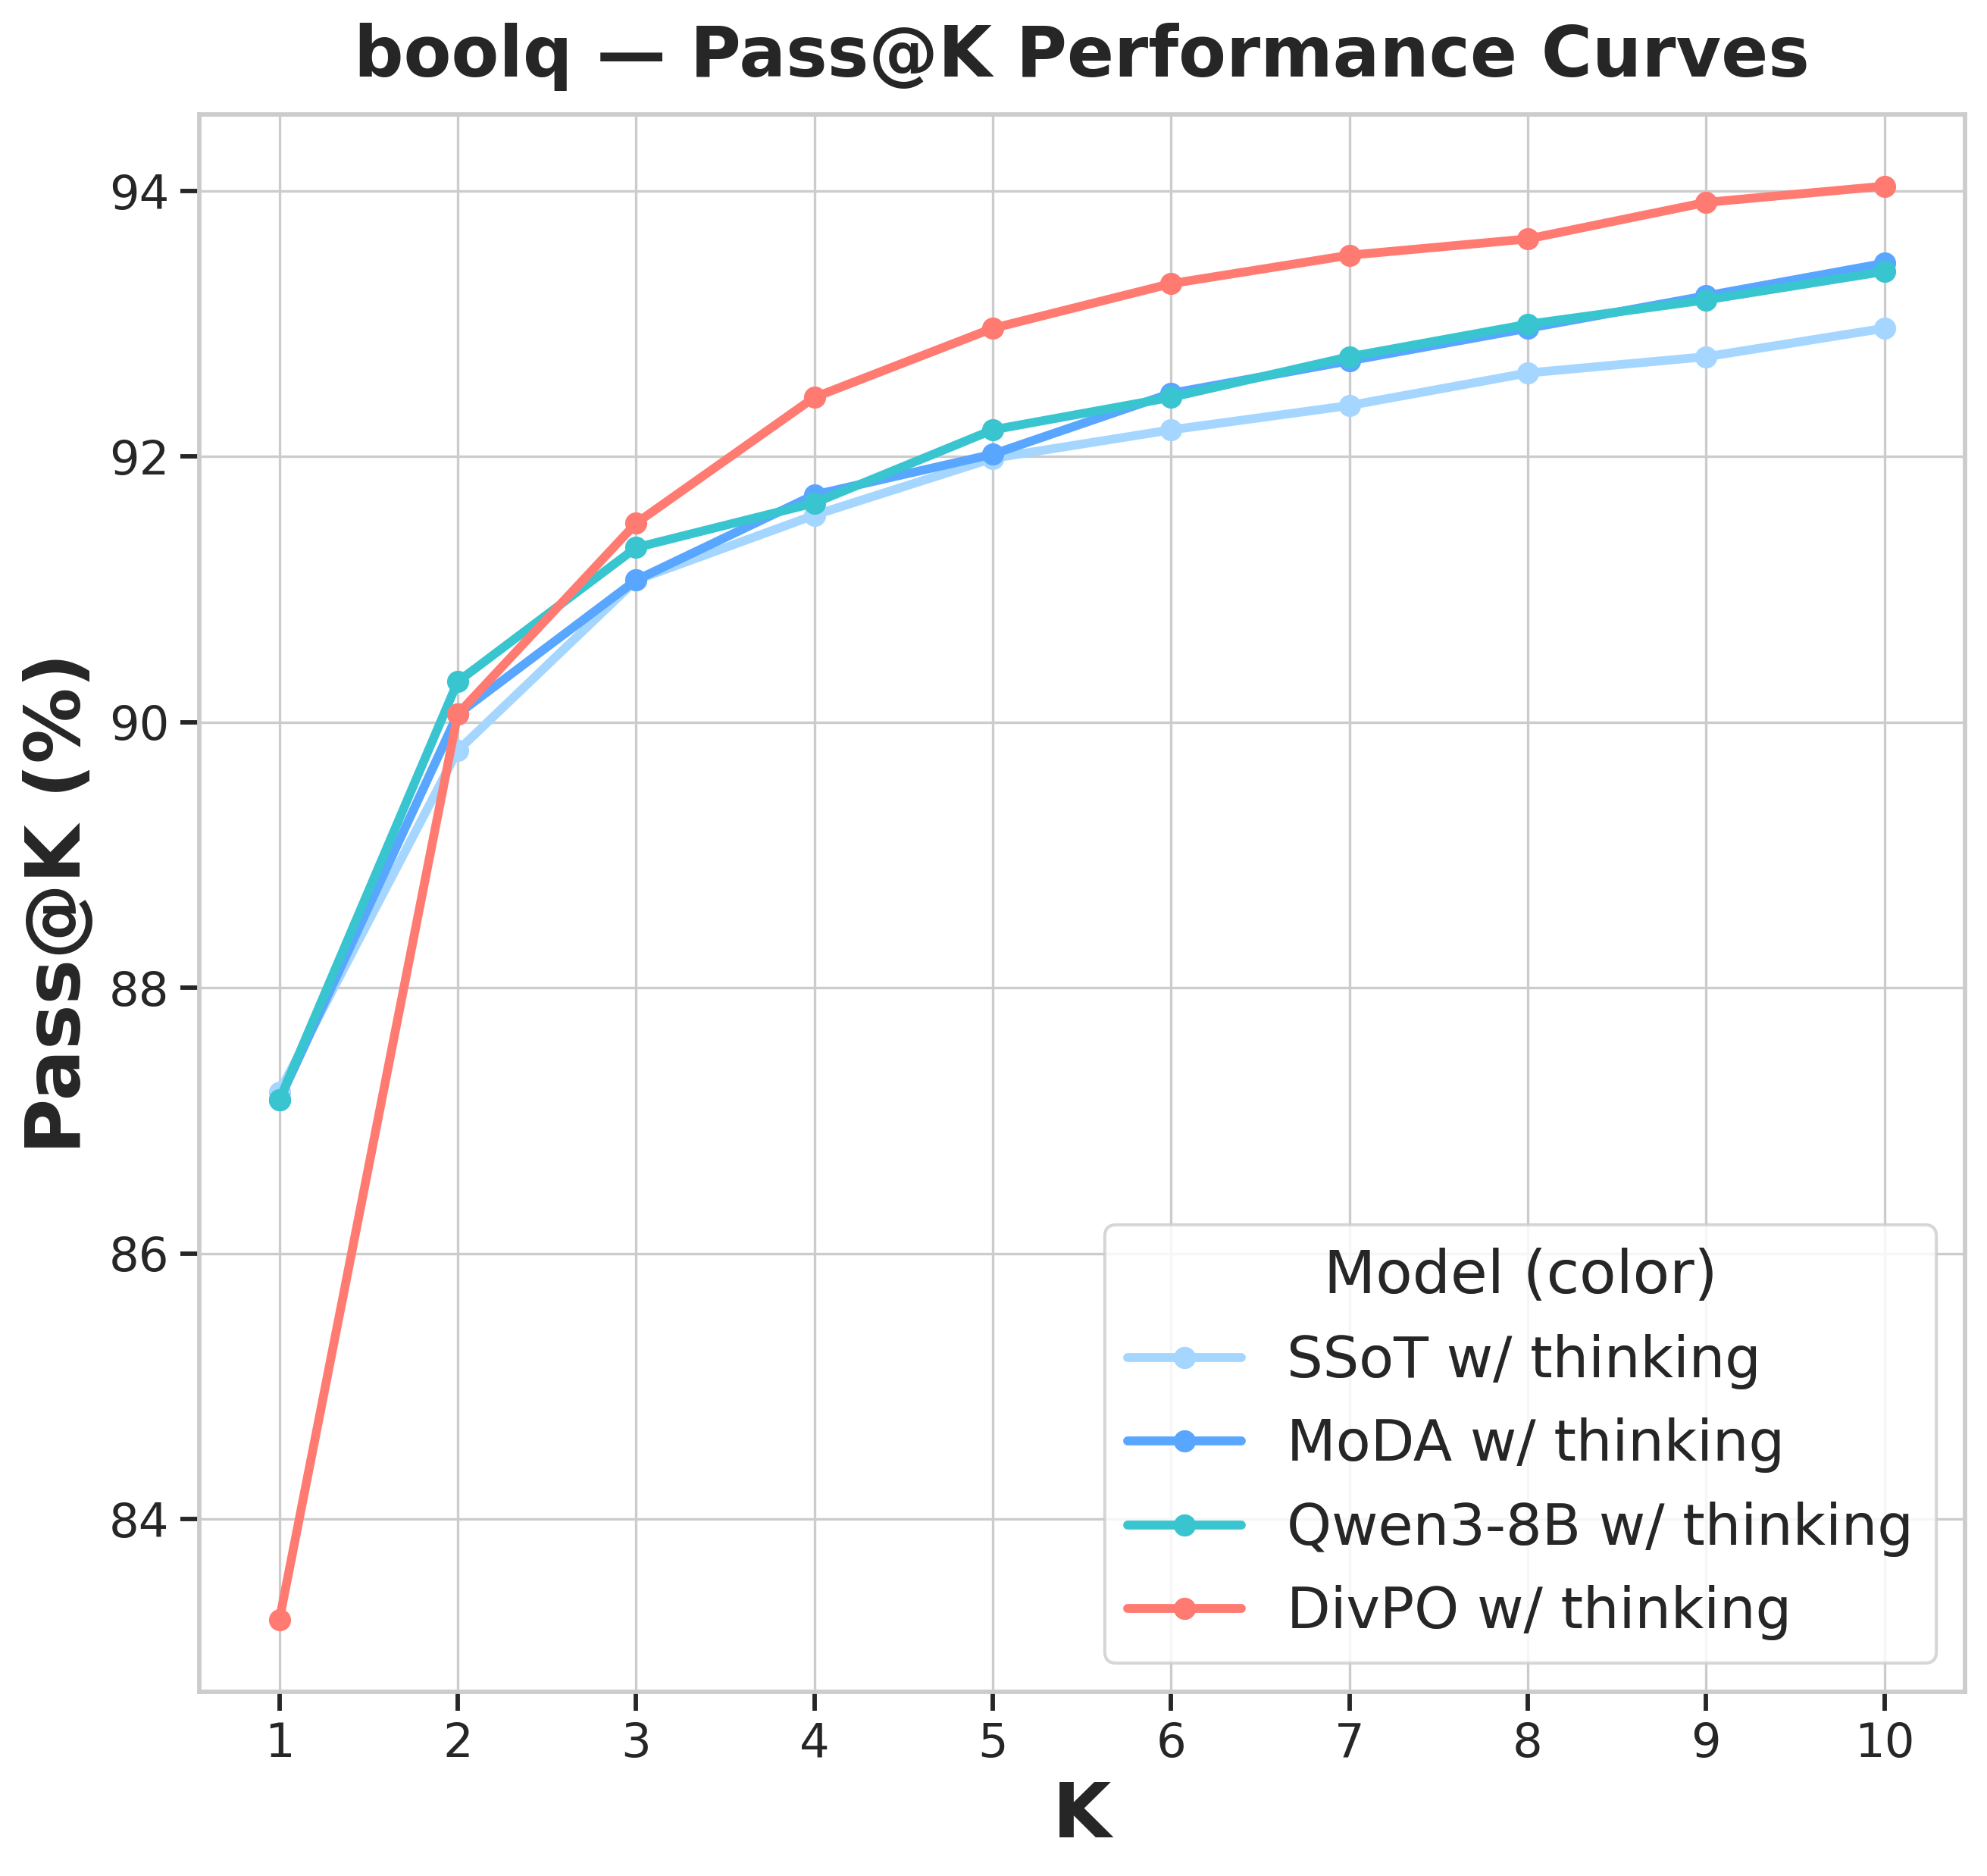
\includegraphics[width=\linewidth]{figures/main_pass_k/pass_at_k_figures/pass_at_k_boolq_thinking_true.png}
\end{minipage}\hfill
\centering
\begin{minipage}{0.24\textwidth}
  \centering
  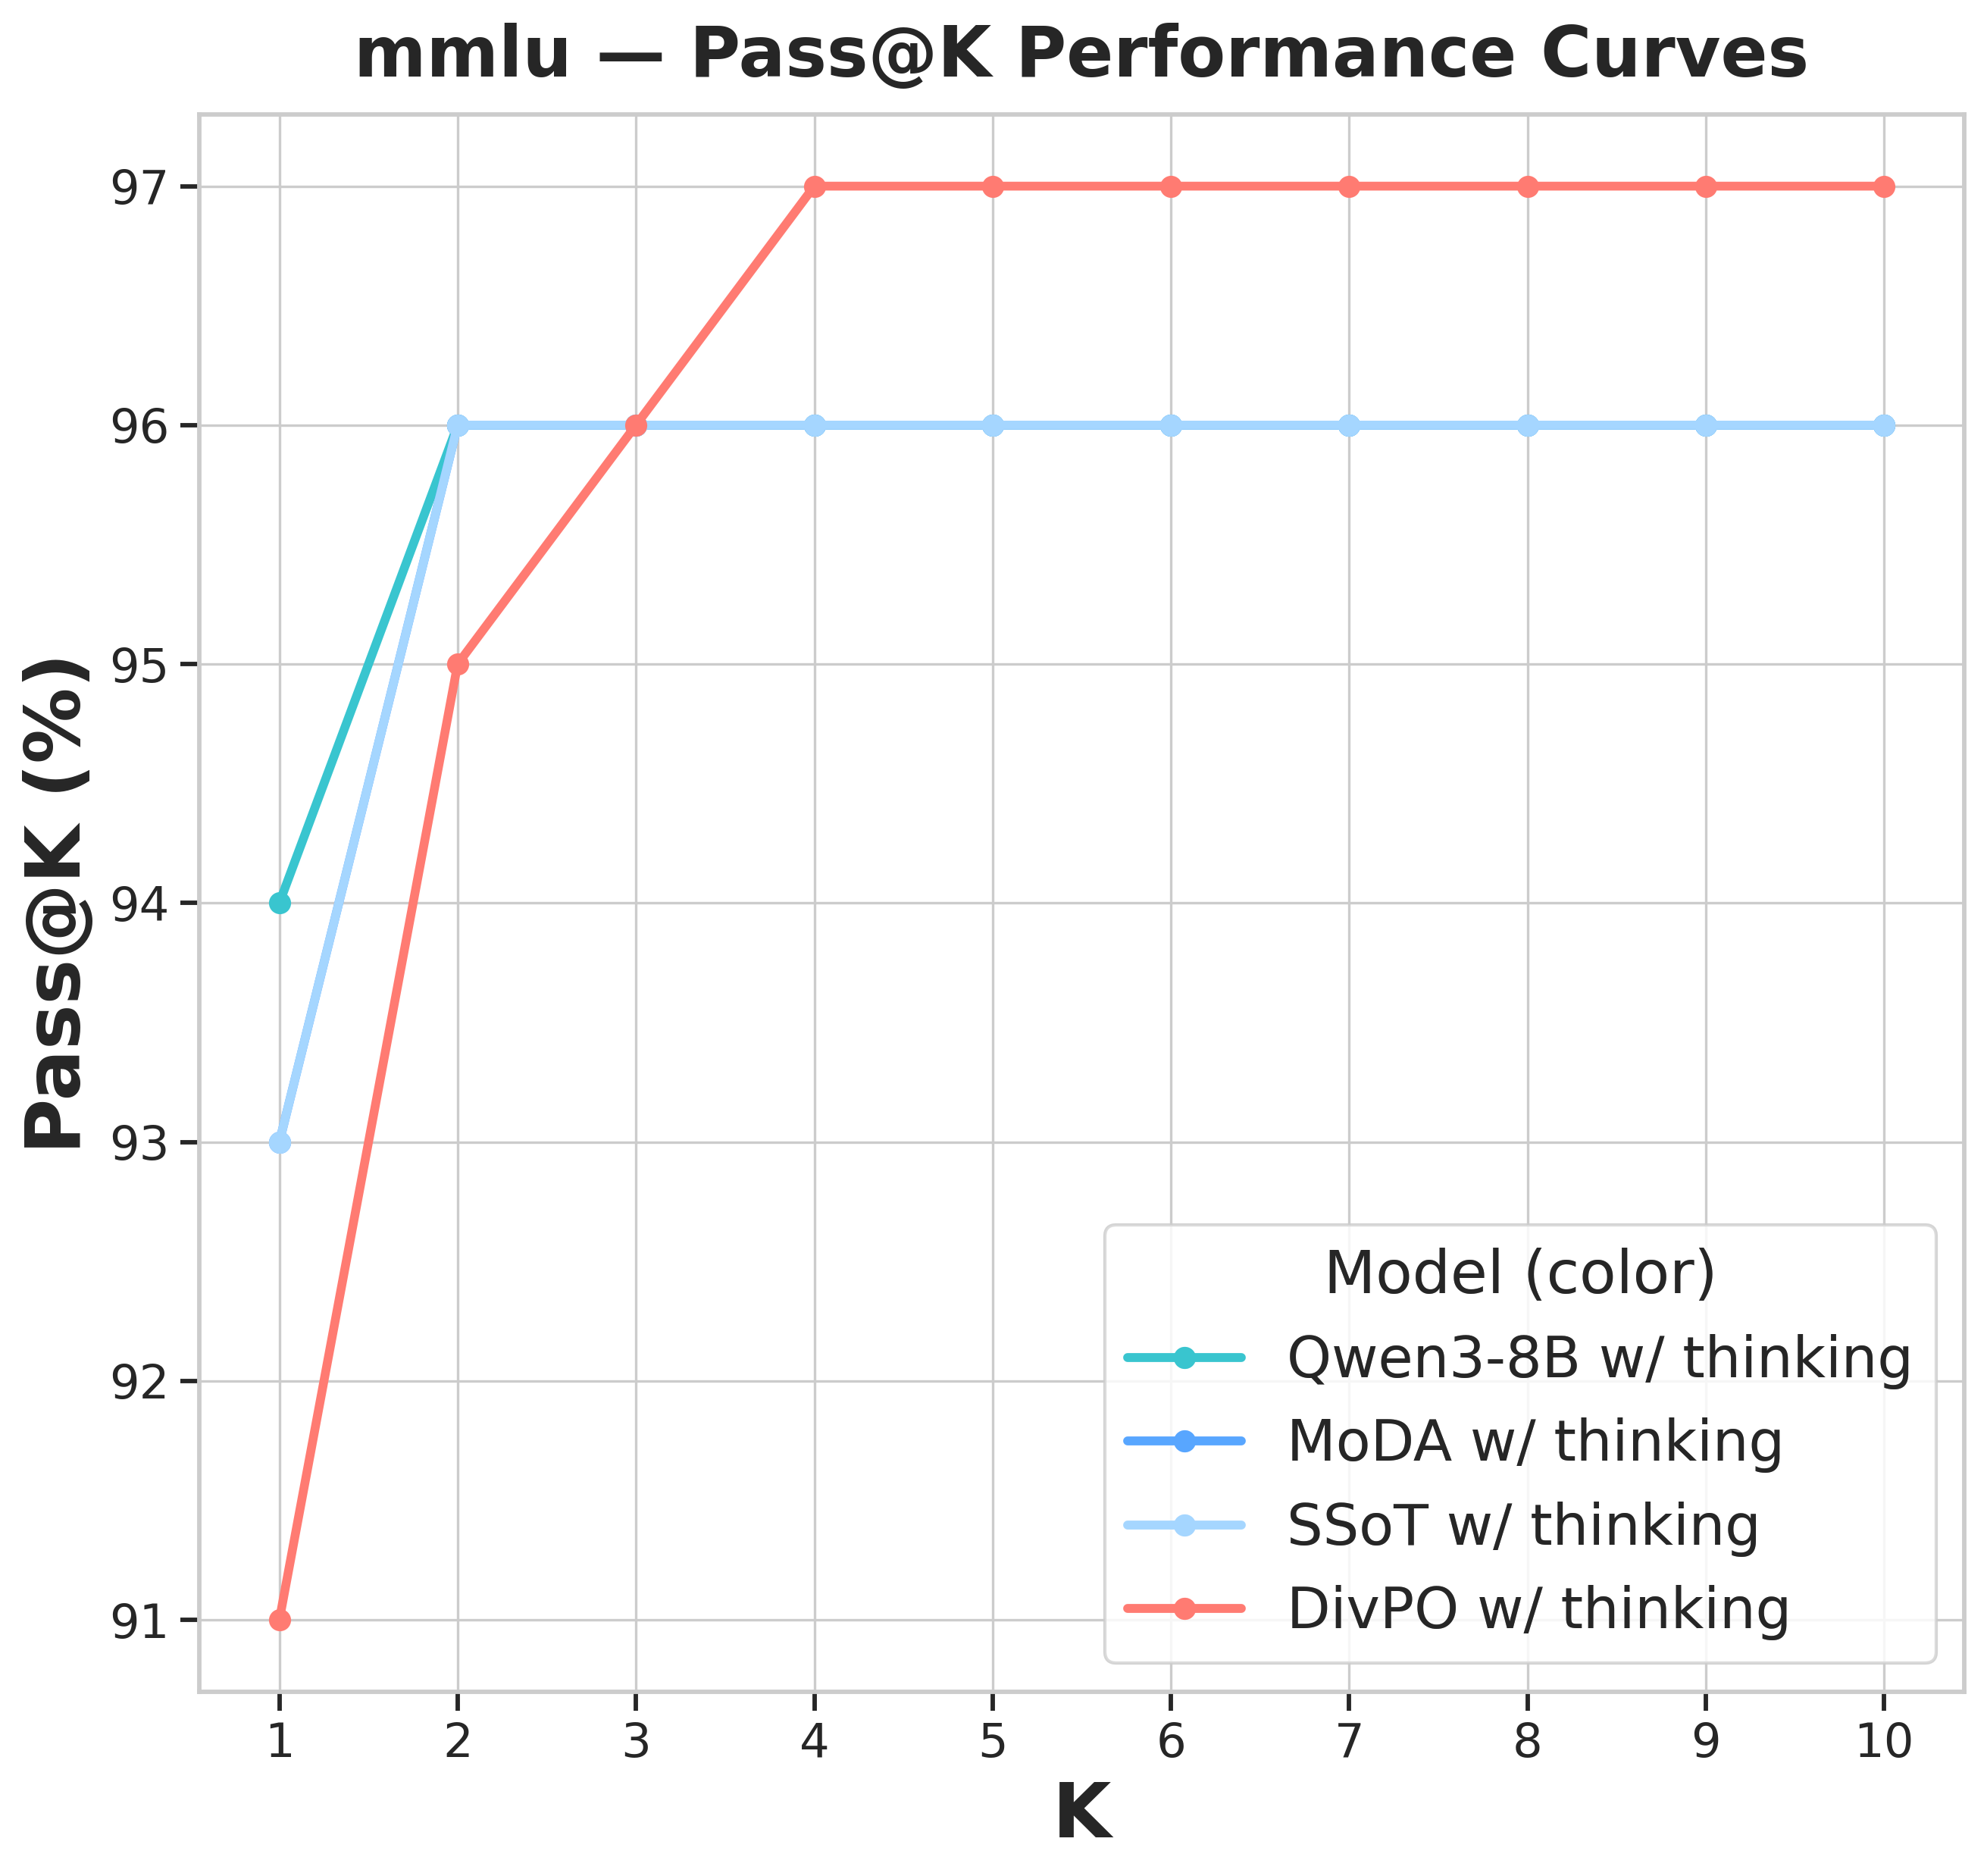
\includegraphics[width=\linewidth]{figures/main_pass_k/pass_at_k_figures/pass_at_k_mmlu_thinking_true.png}
\end{minipage}\hfill
\begin{minipage}{0.24\textwidth}
  \centering
  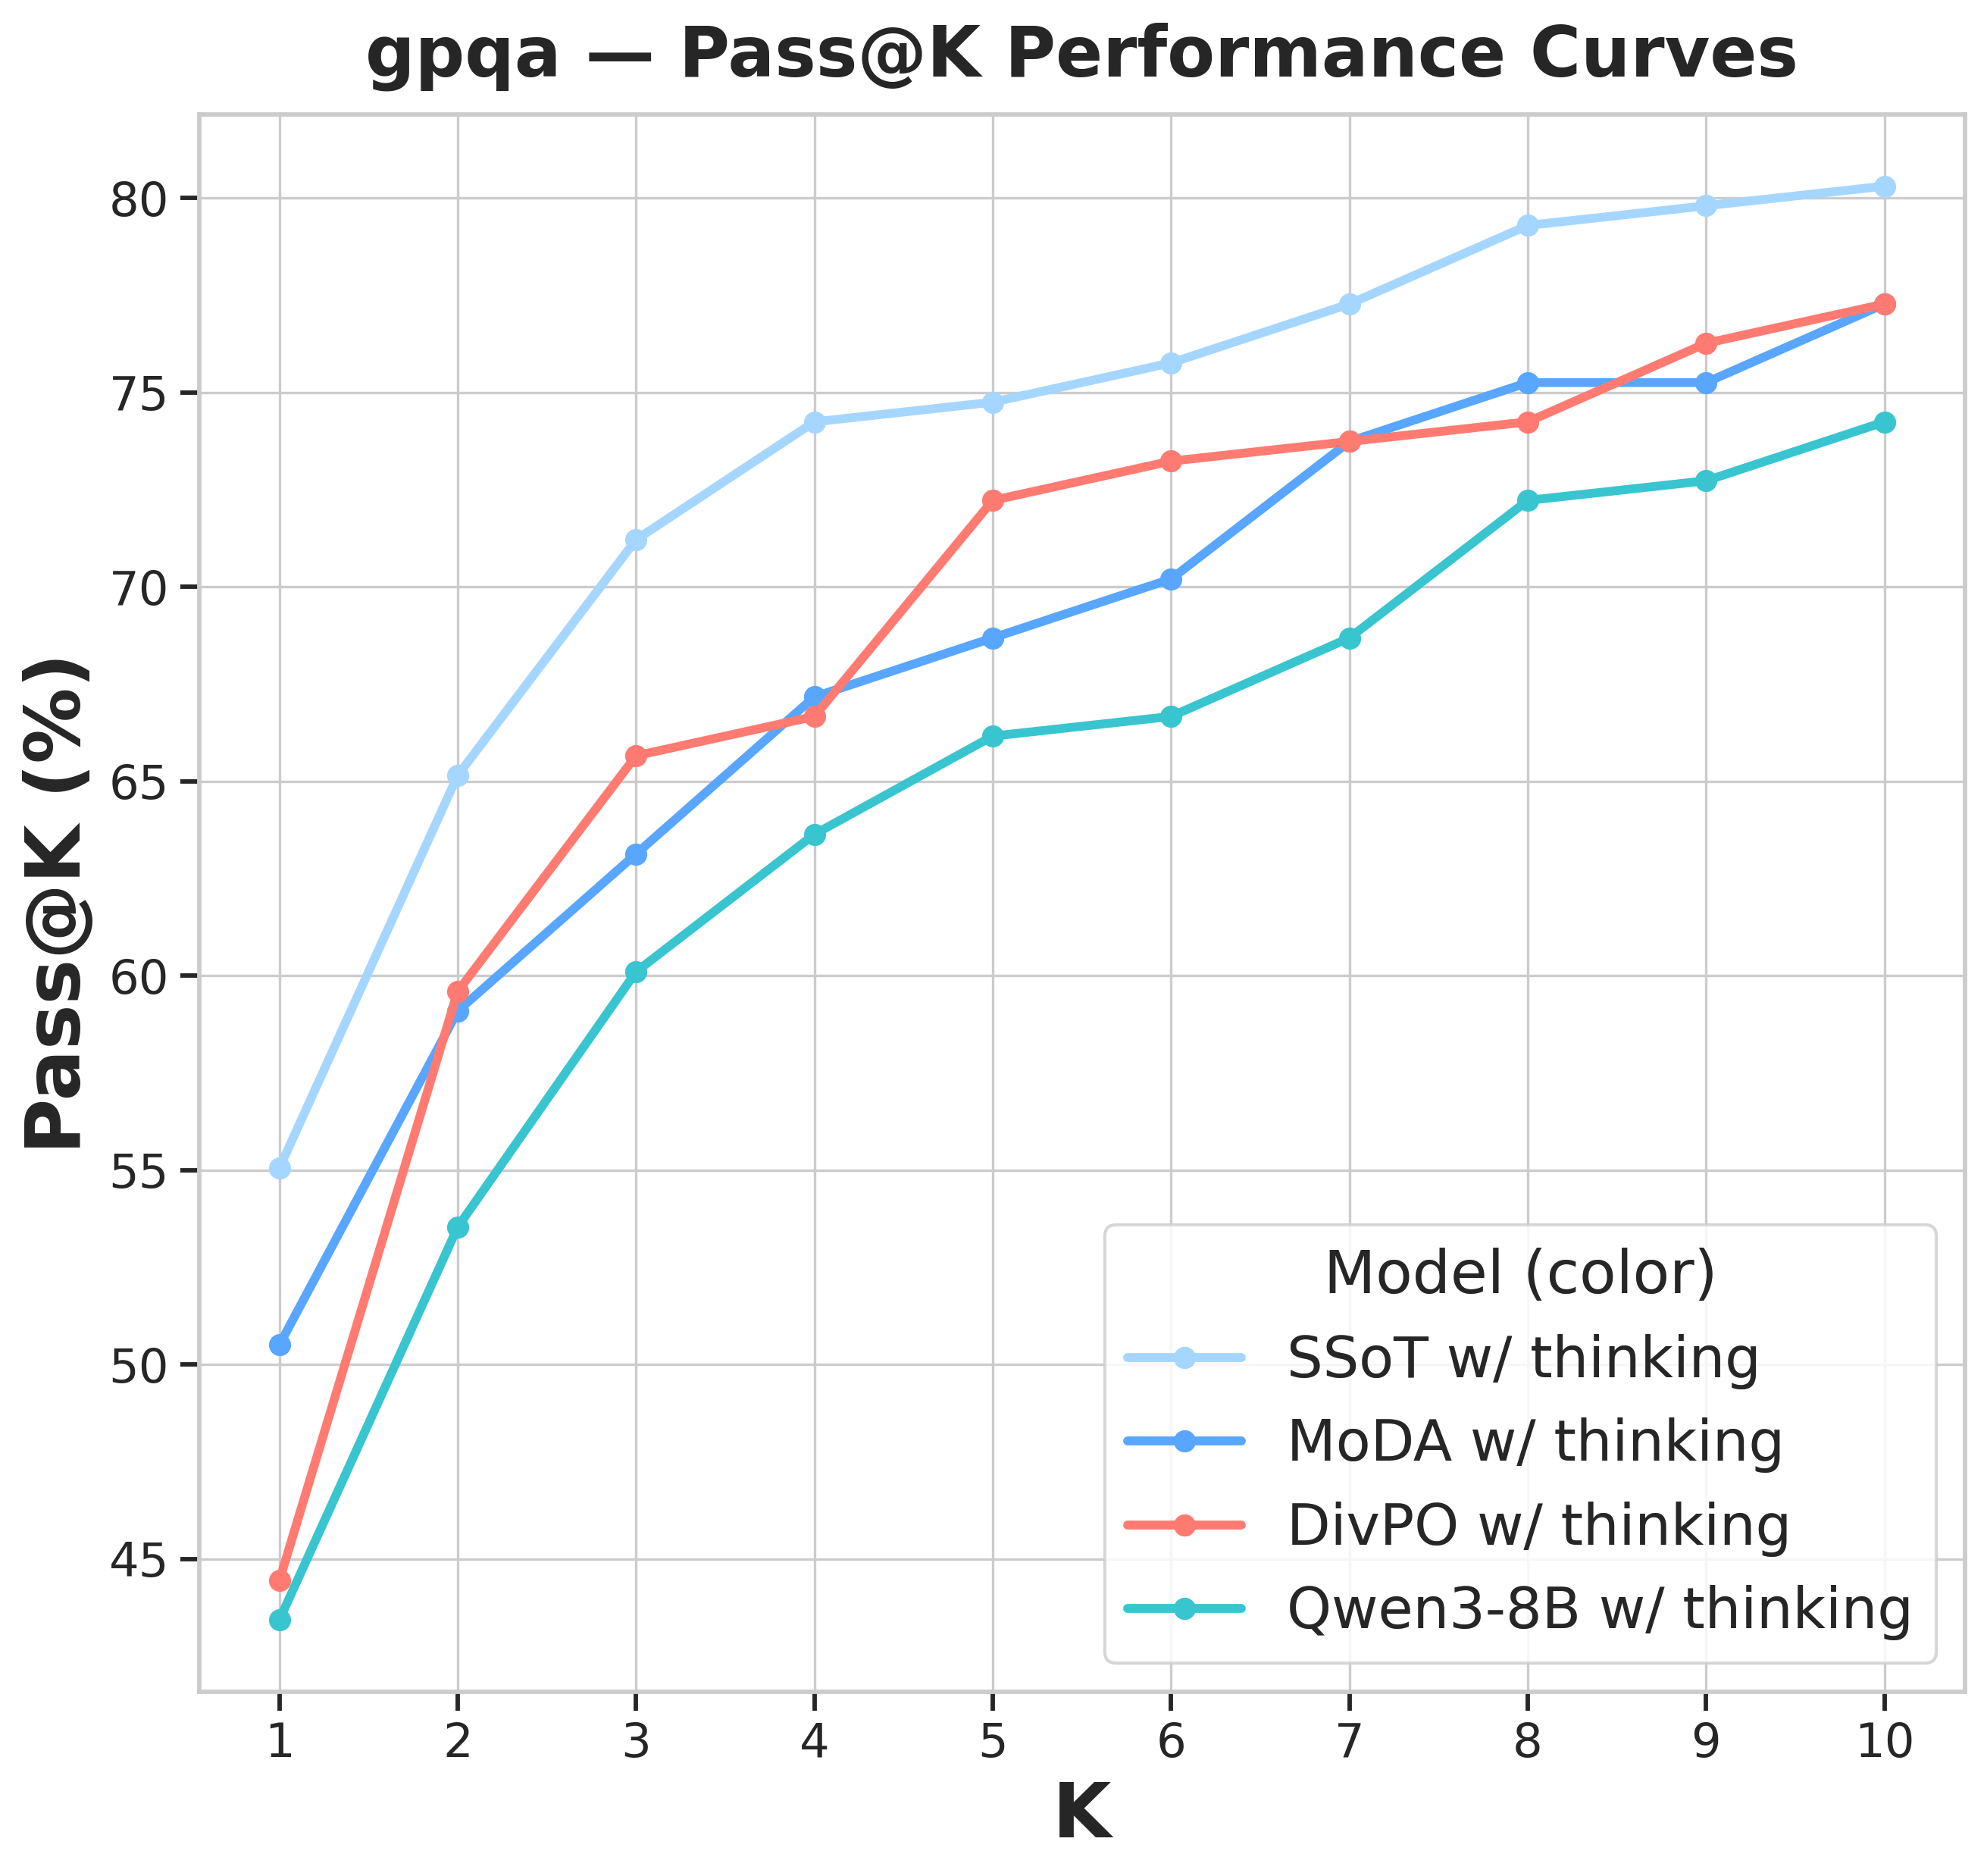
\includegraphics[width=\linewidth]{figures/main_pass_k/pass_at_k_figures/pass_at_k_gpqa_thinking_true.png}
\end{minipage}\hfill
\begin{minipage}{0.24\textwidth}
  \centering
  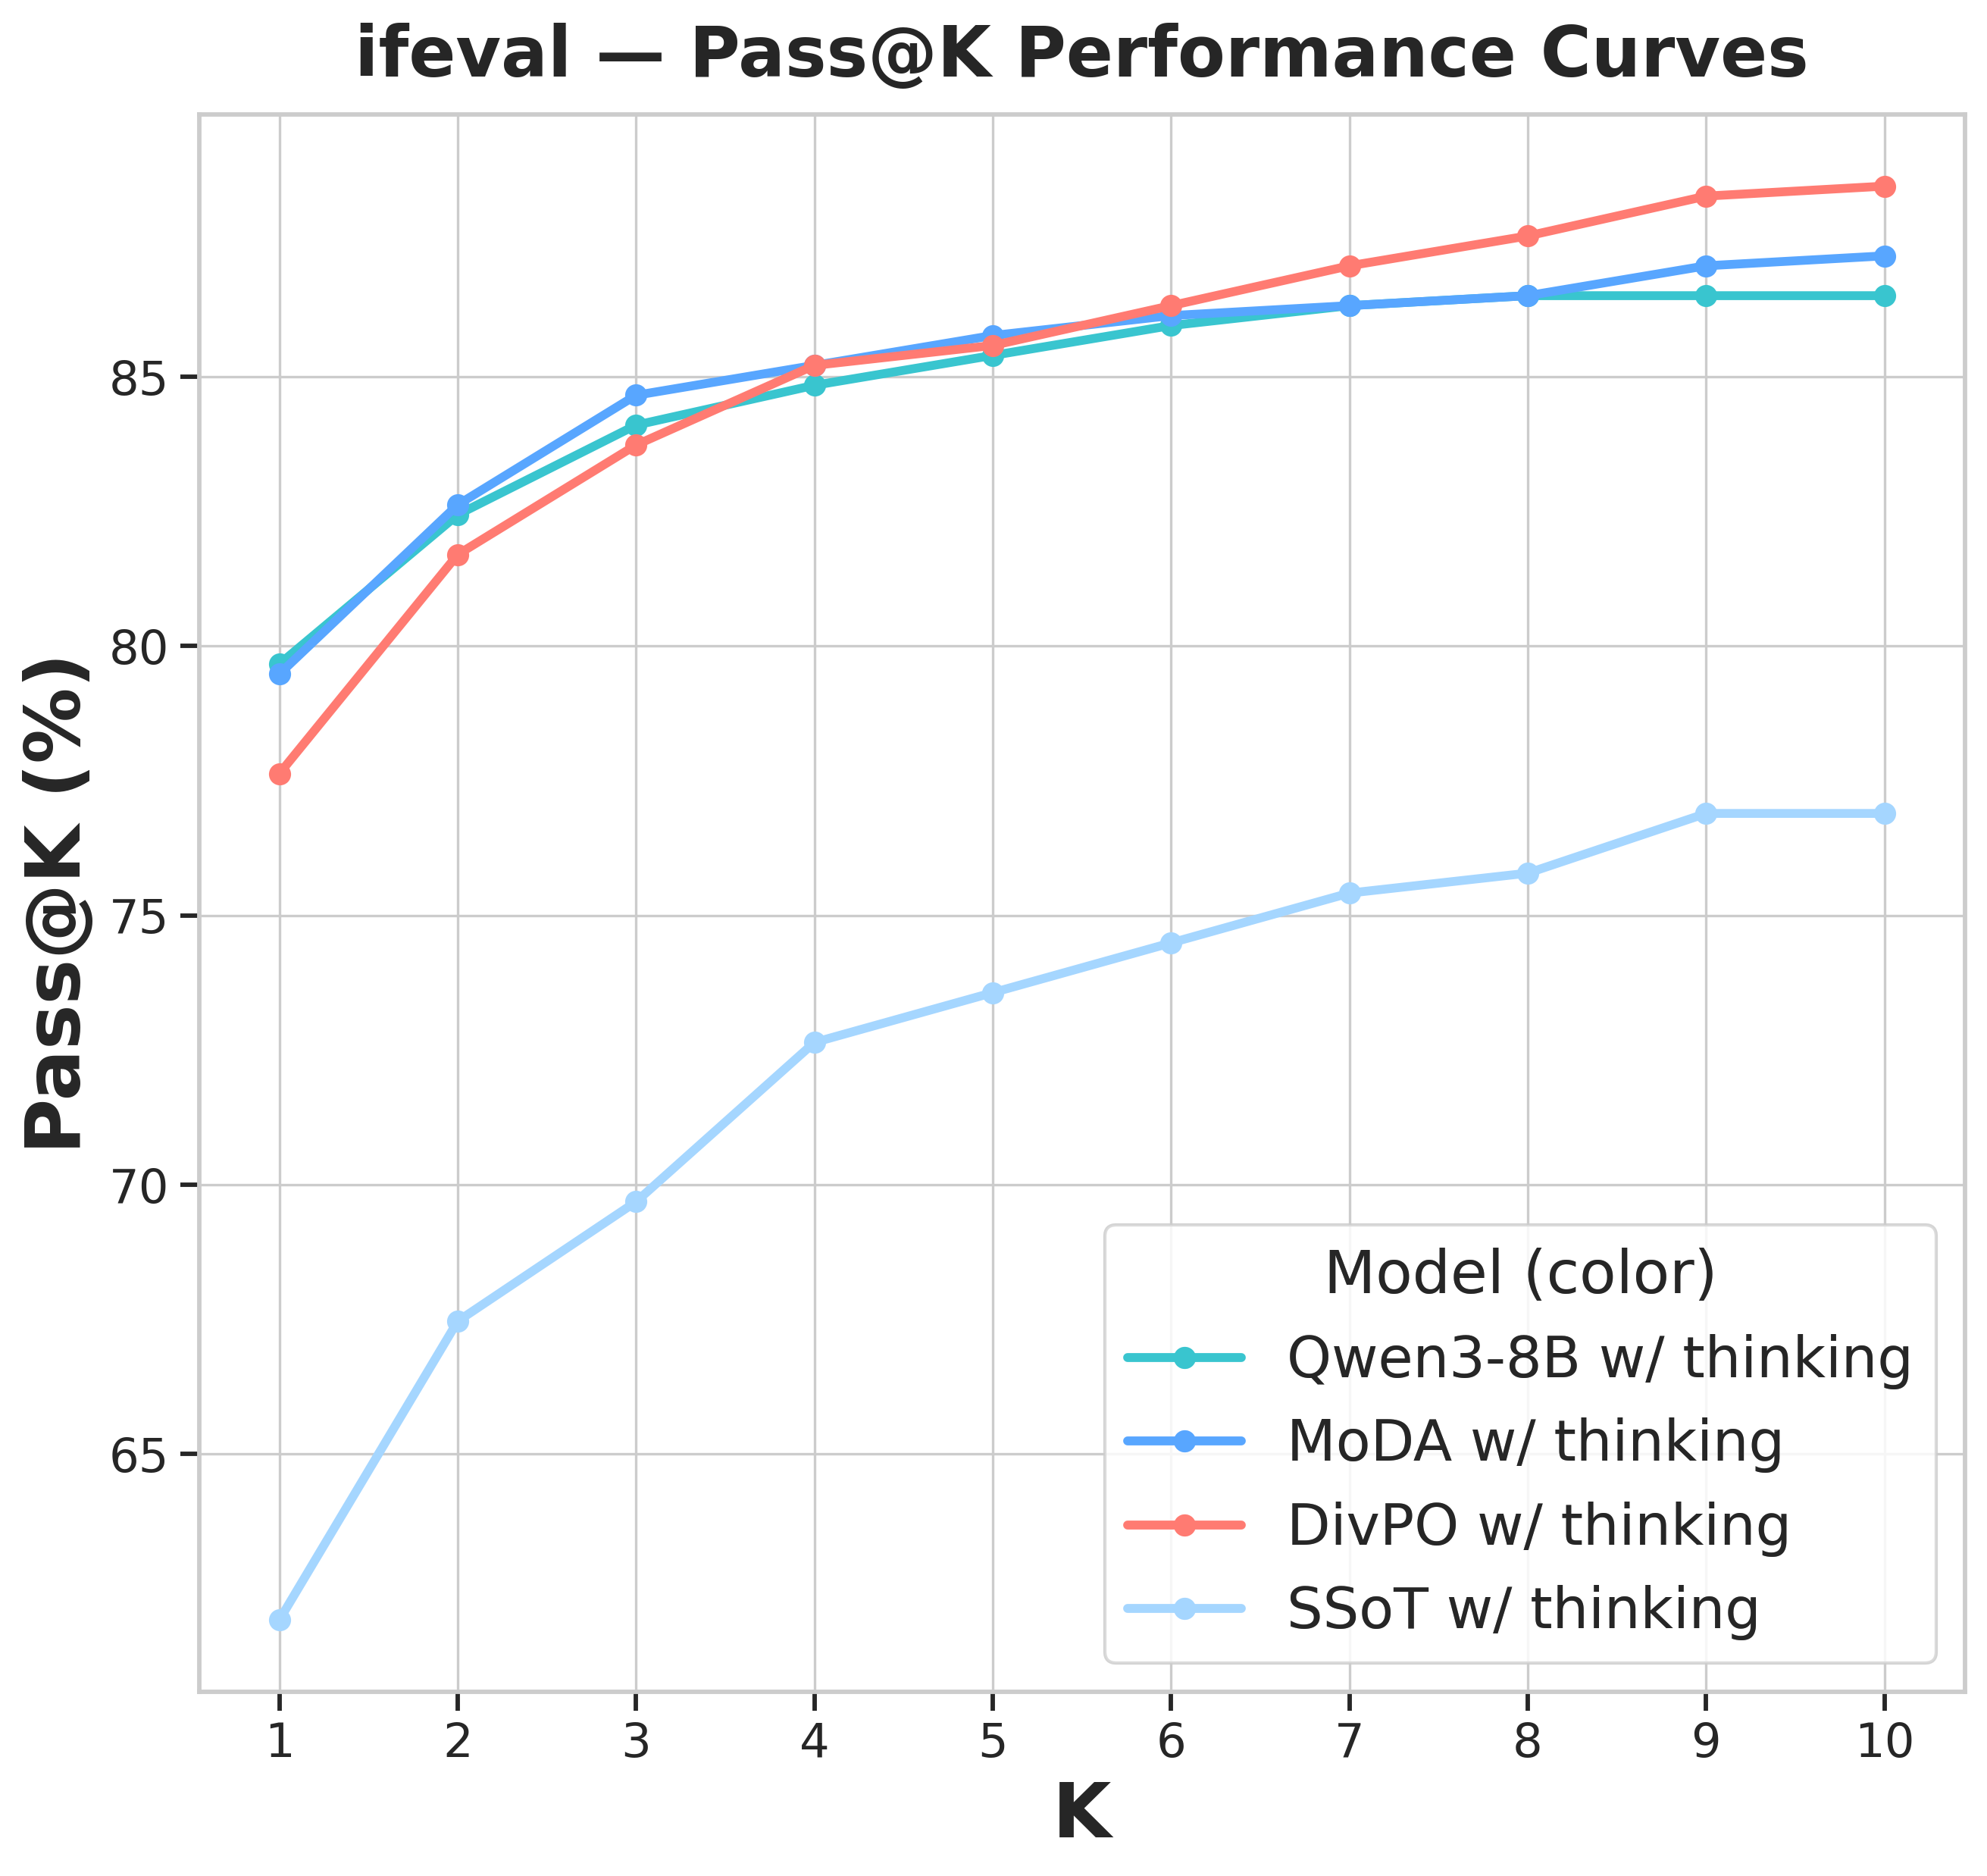
\includegraphics[width=\linewidth]{figures/main_pass_k/pass_at_k_figures/pass_at_k_ifeval_thinking_true.png}
\end{minipage}
\caption{\textbf{General capability retention: pass@k accuracy.} Qwen3-8B base and thinking enabled models.}
\label{fig:general capability pass@k thinking enabled}
\end{figure}


\begin{figure}[H]
\begin{minipage}{0.24\textwidth}
  \centering
  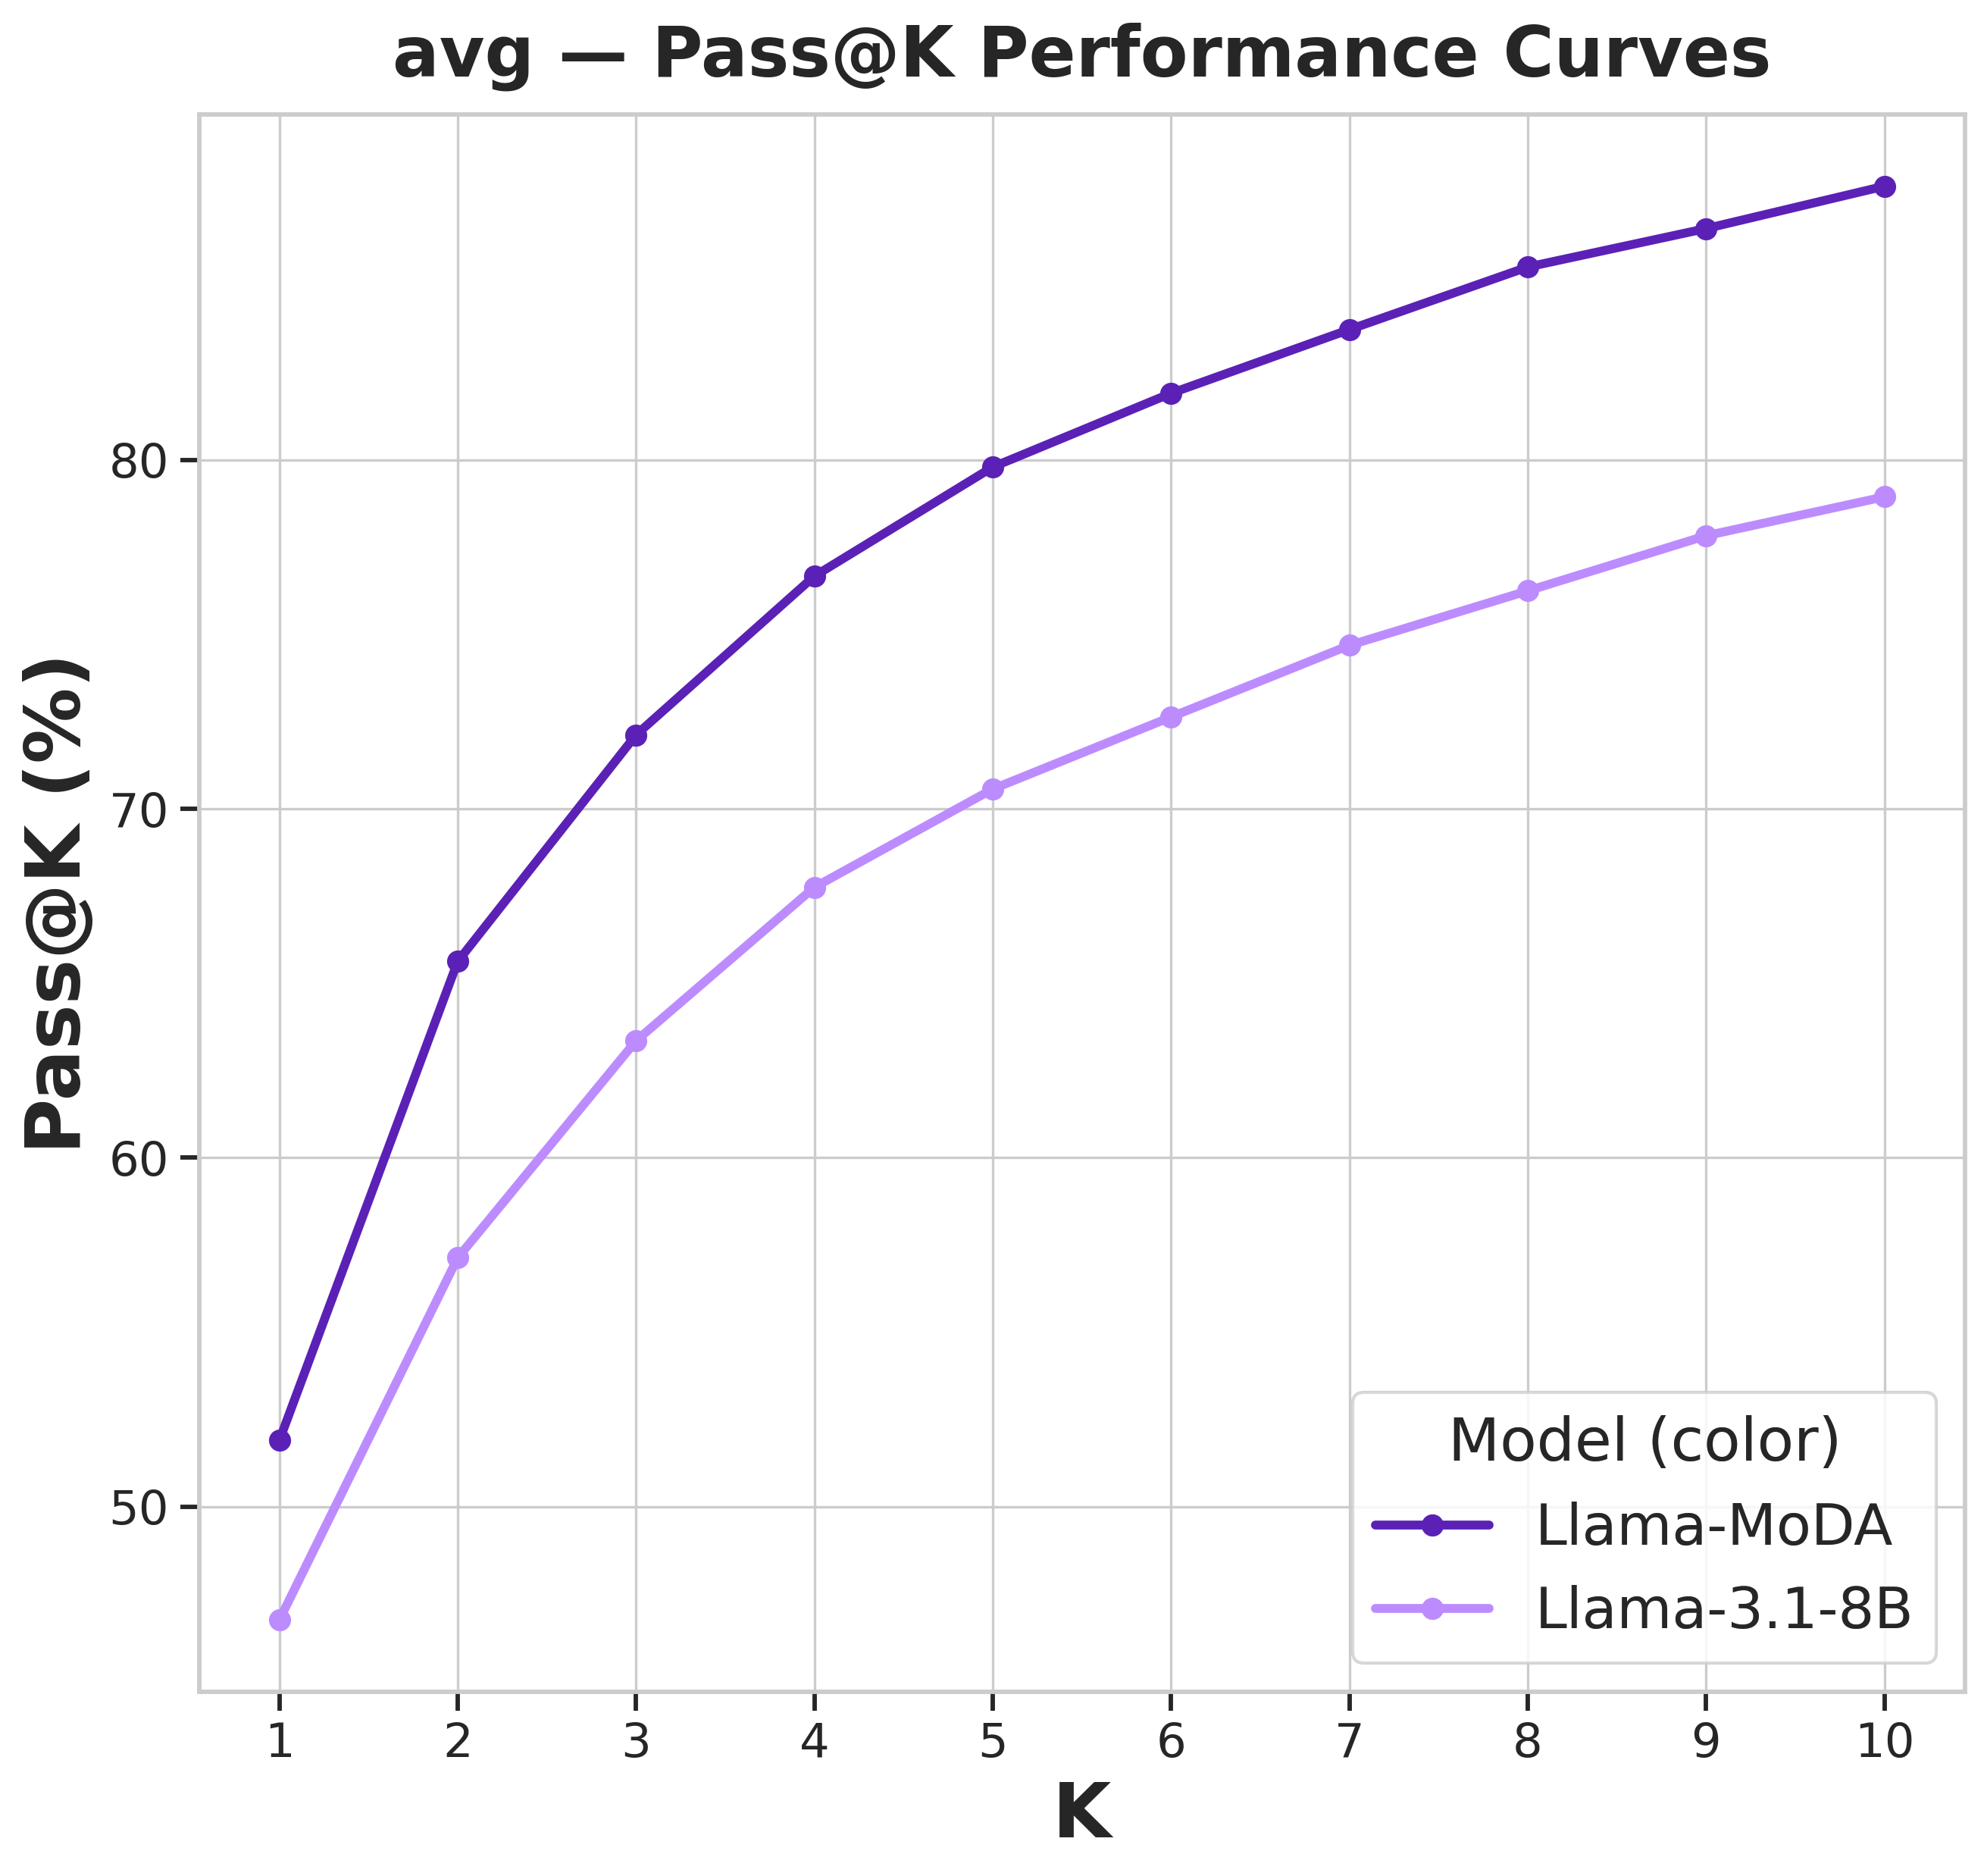
\includegraphics[width=\linewidth]{figures/main_pass_k/pass_at_k_figures/pass_at_k_avg_thinking_false_base_model_llama3_1-8b.png}
\end{minipage}\hfill
\centering
\begin{minipage}{0.24\textwidth}
  \centering
  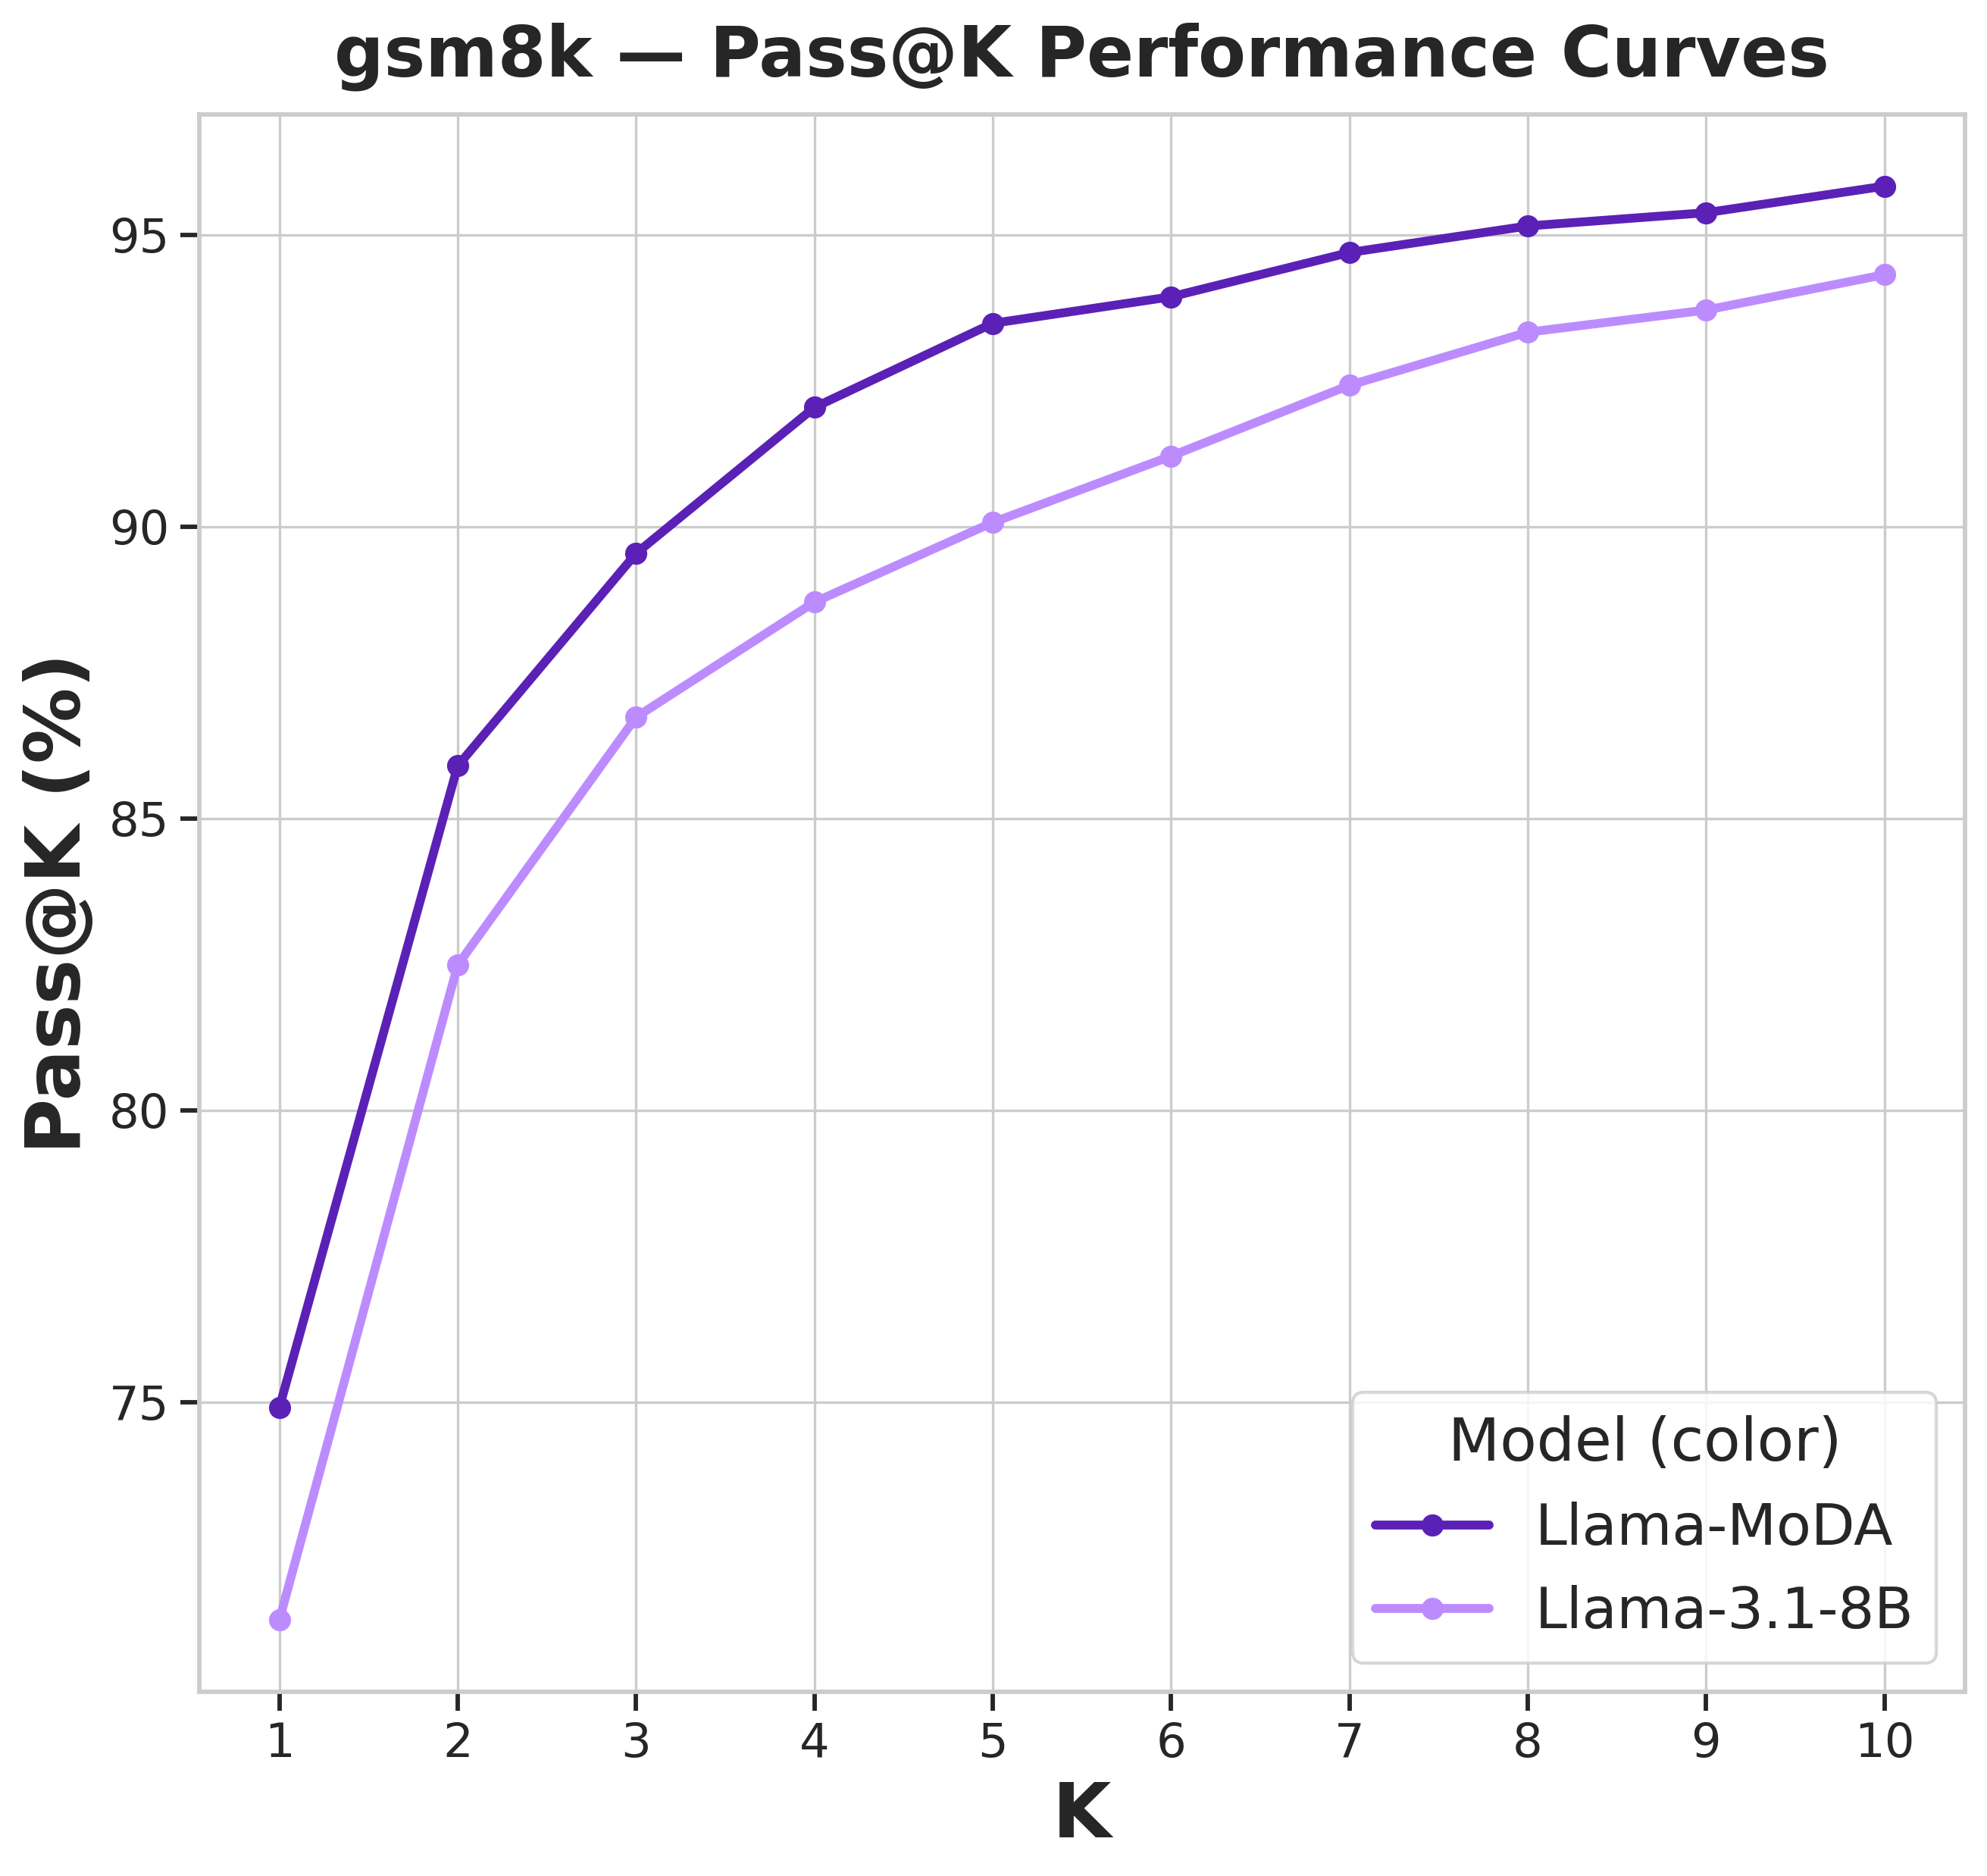
\includegraphics[width=\linewidth]{figures/main_pass_k/pass_at_k_figures/pass_at_k_gsm8k_thinking_false_base_model_llama3_1-8b.png}
\end{minipage}\hfill
\begin{minipage}{0.24\textwidth}
  \centering
  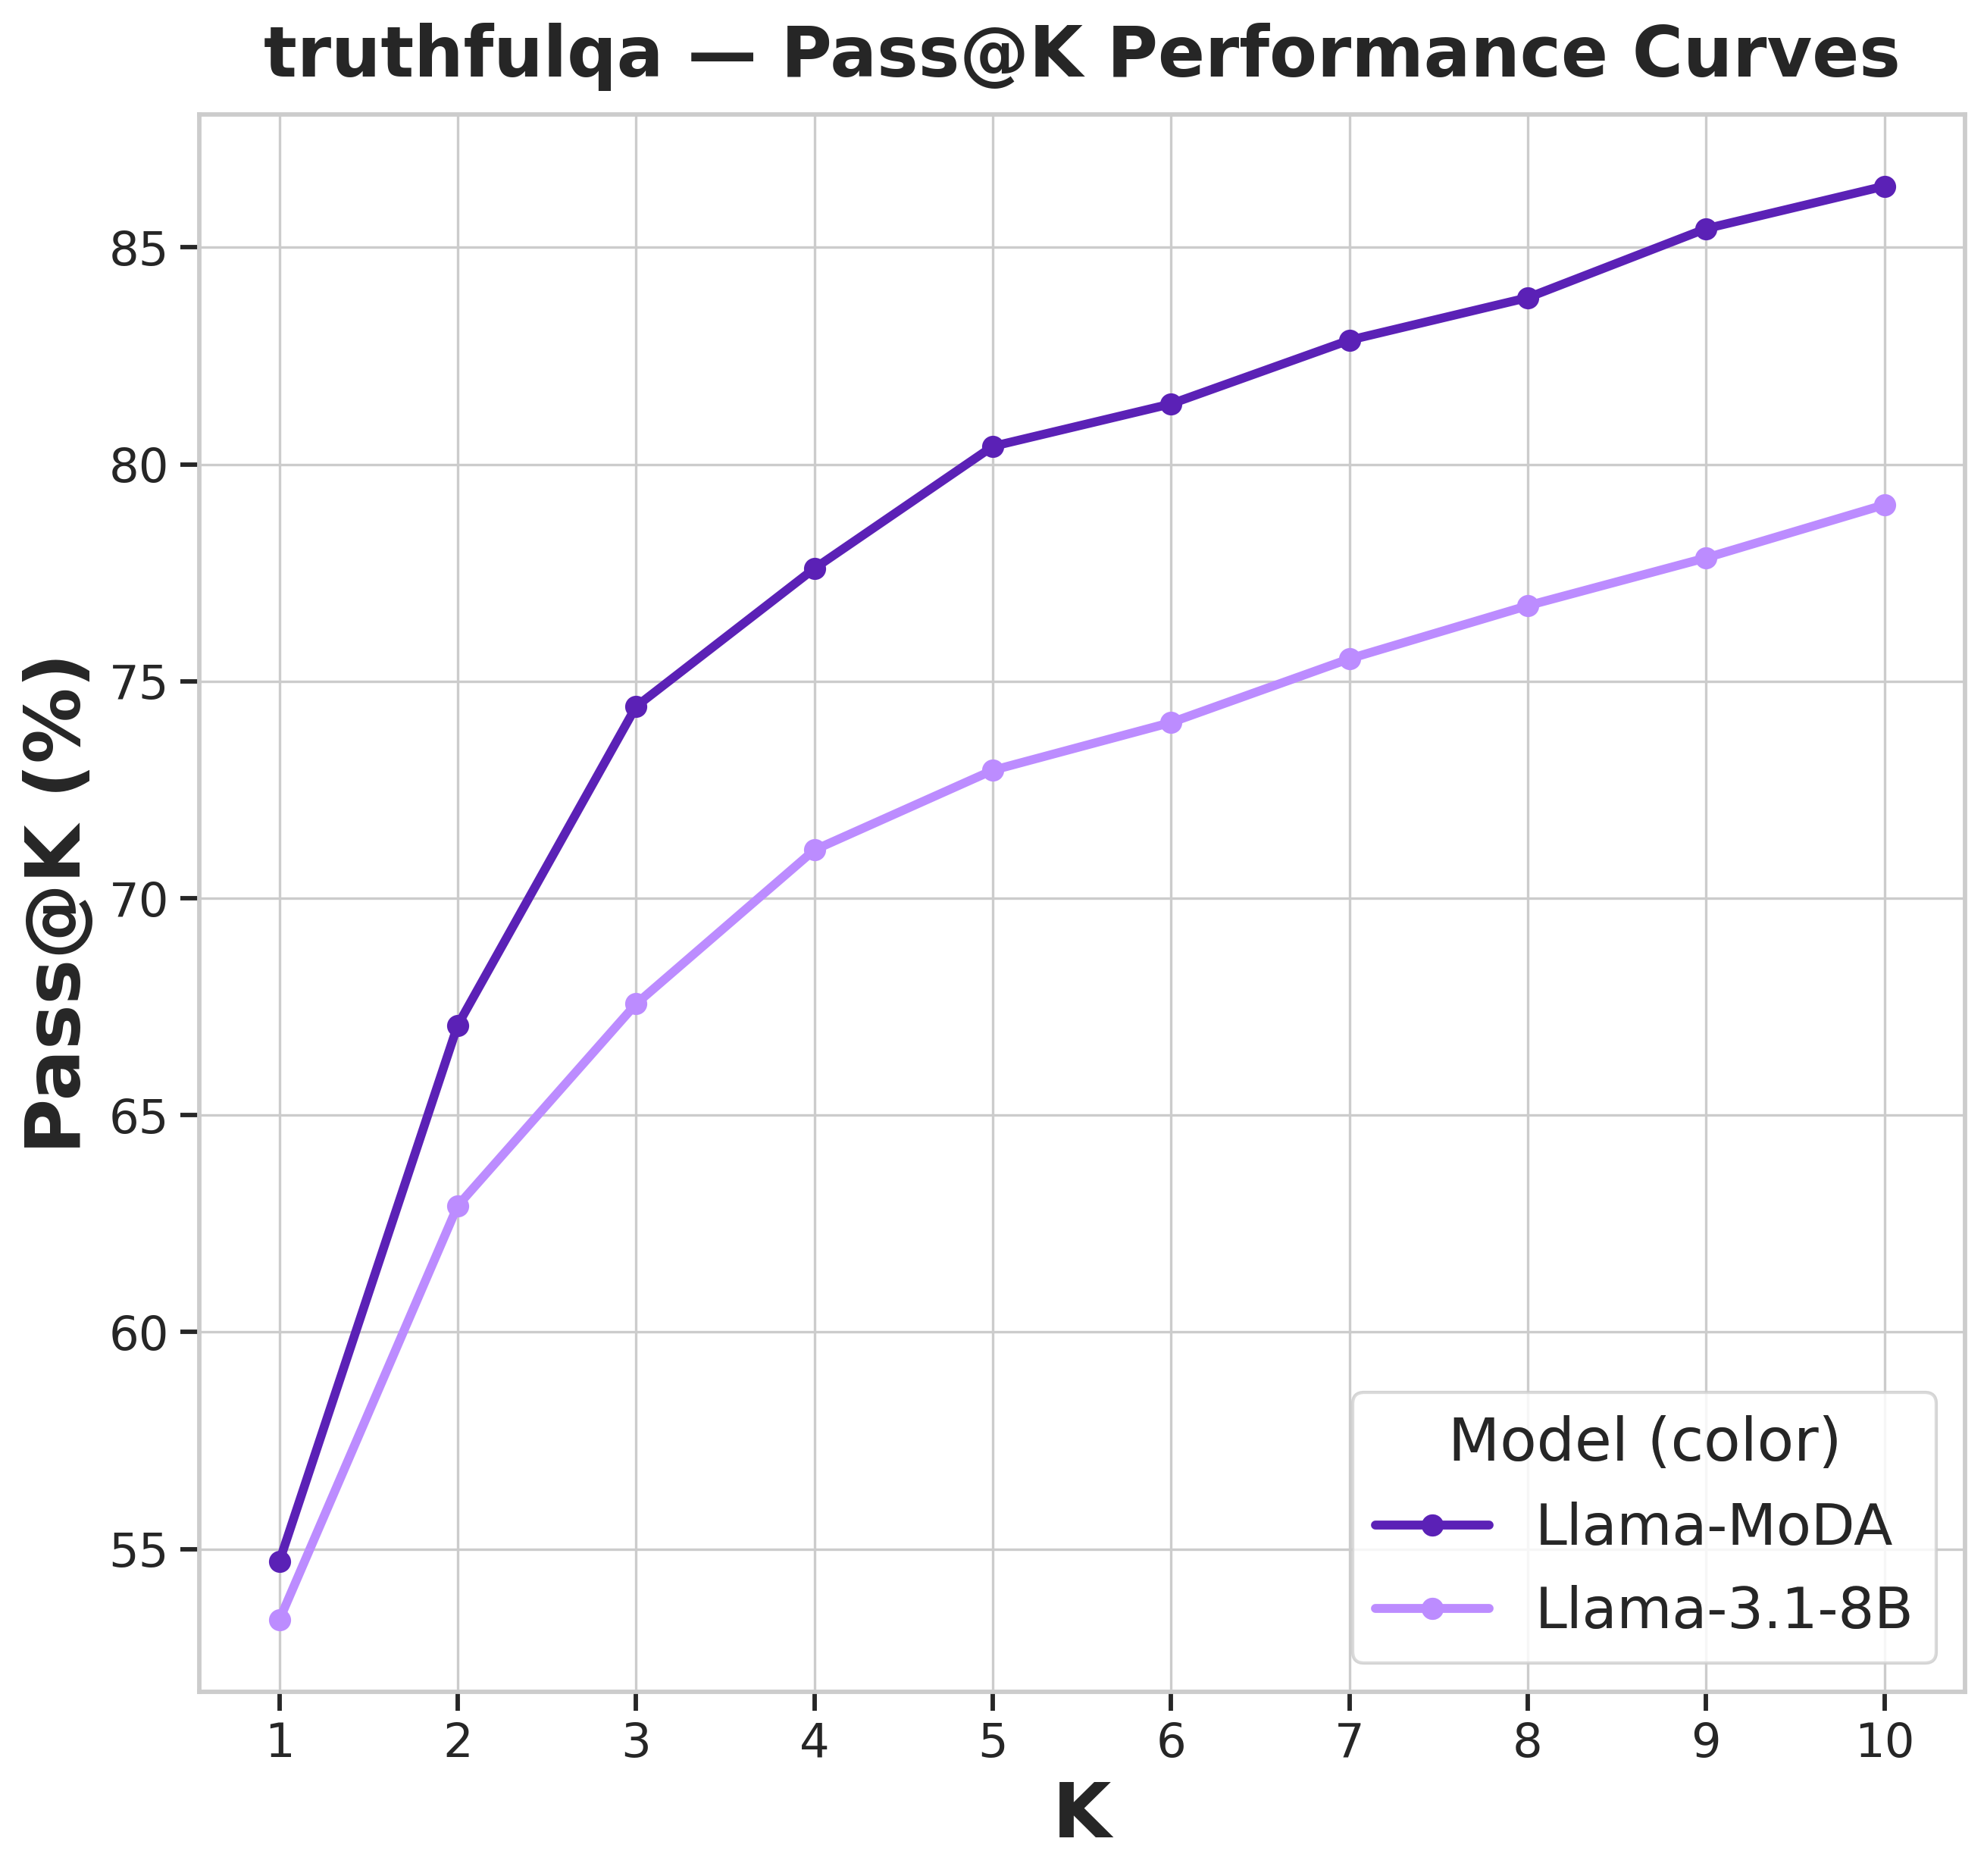
\includegraphics[width=\linewidth]{figures/main_pass_k/pass_at_k_figures/pass_at_k_truthfulqa_thinking_false_base_model_llama3_1-8b.png}
\end{minipage}\hfill
\begin{minipage}{0.24\textwidth}
  \centering
  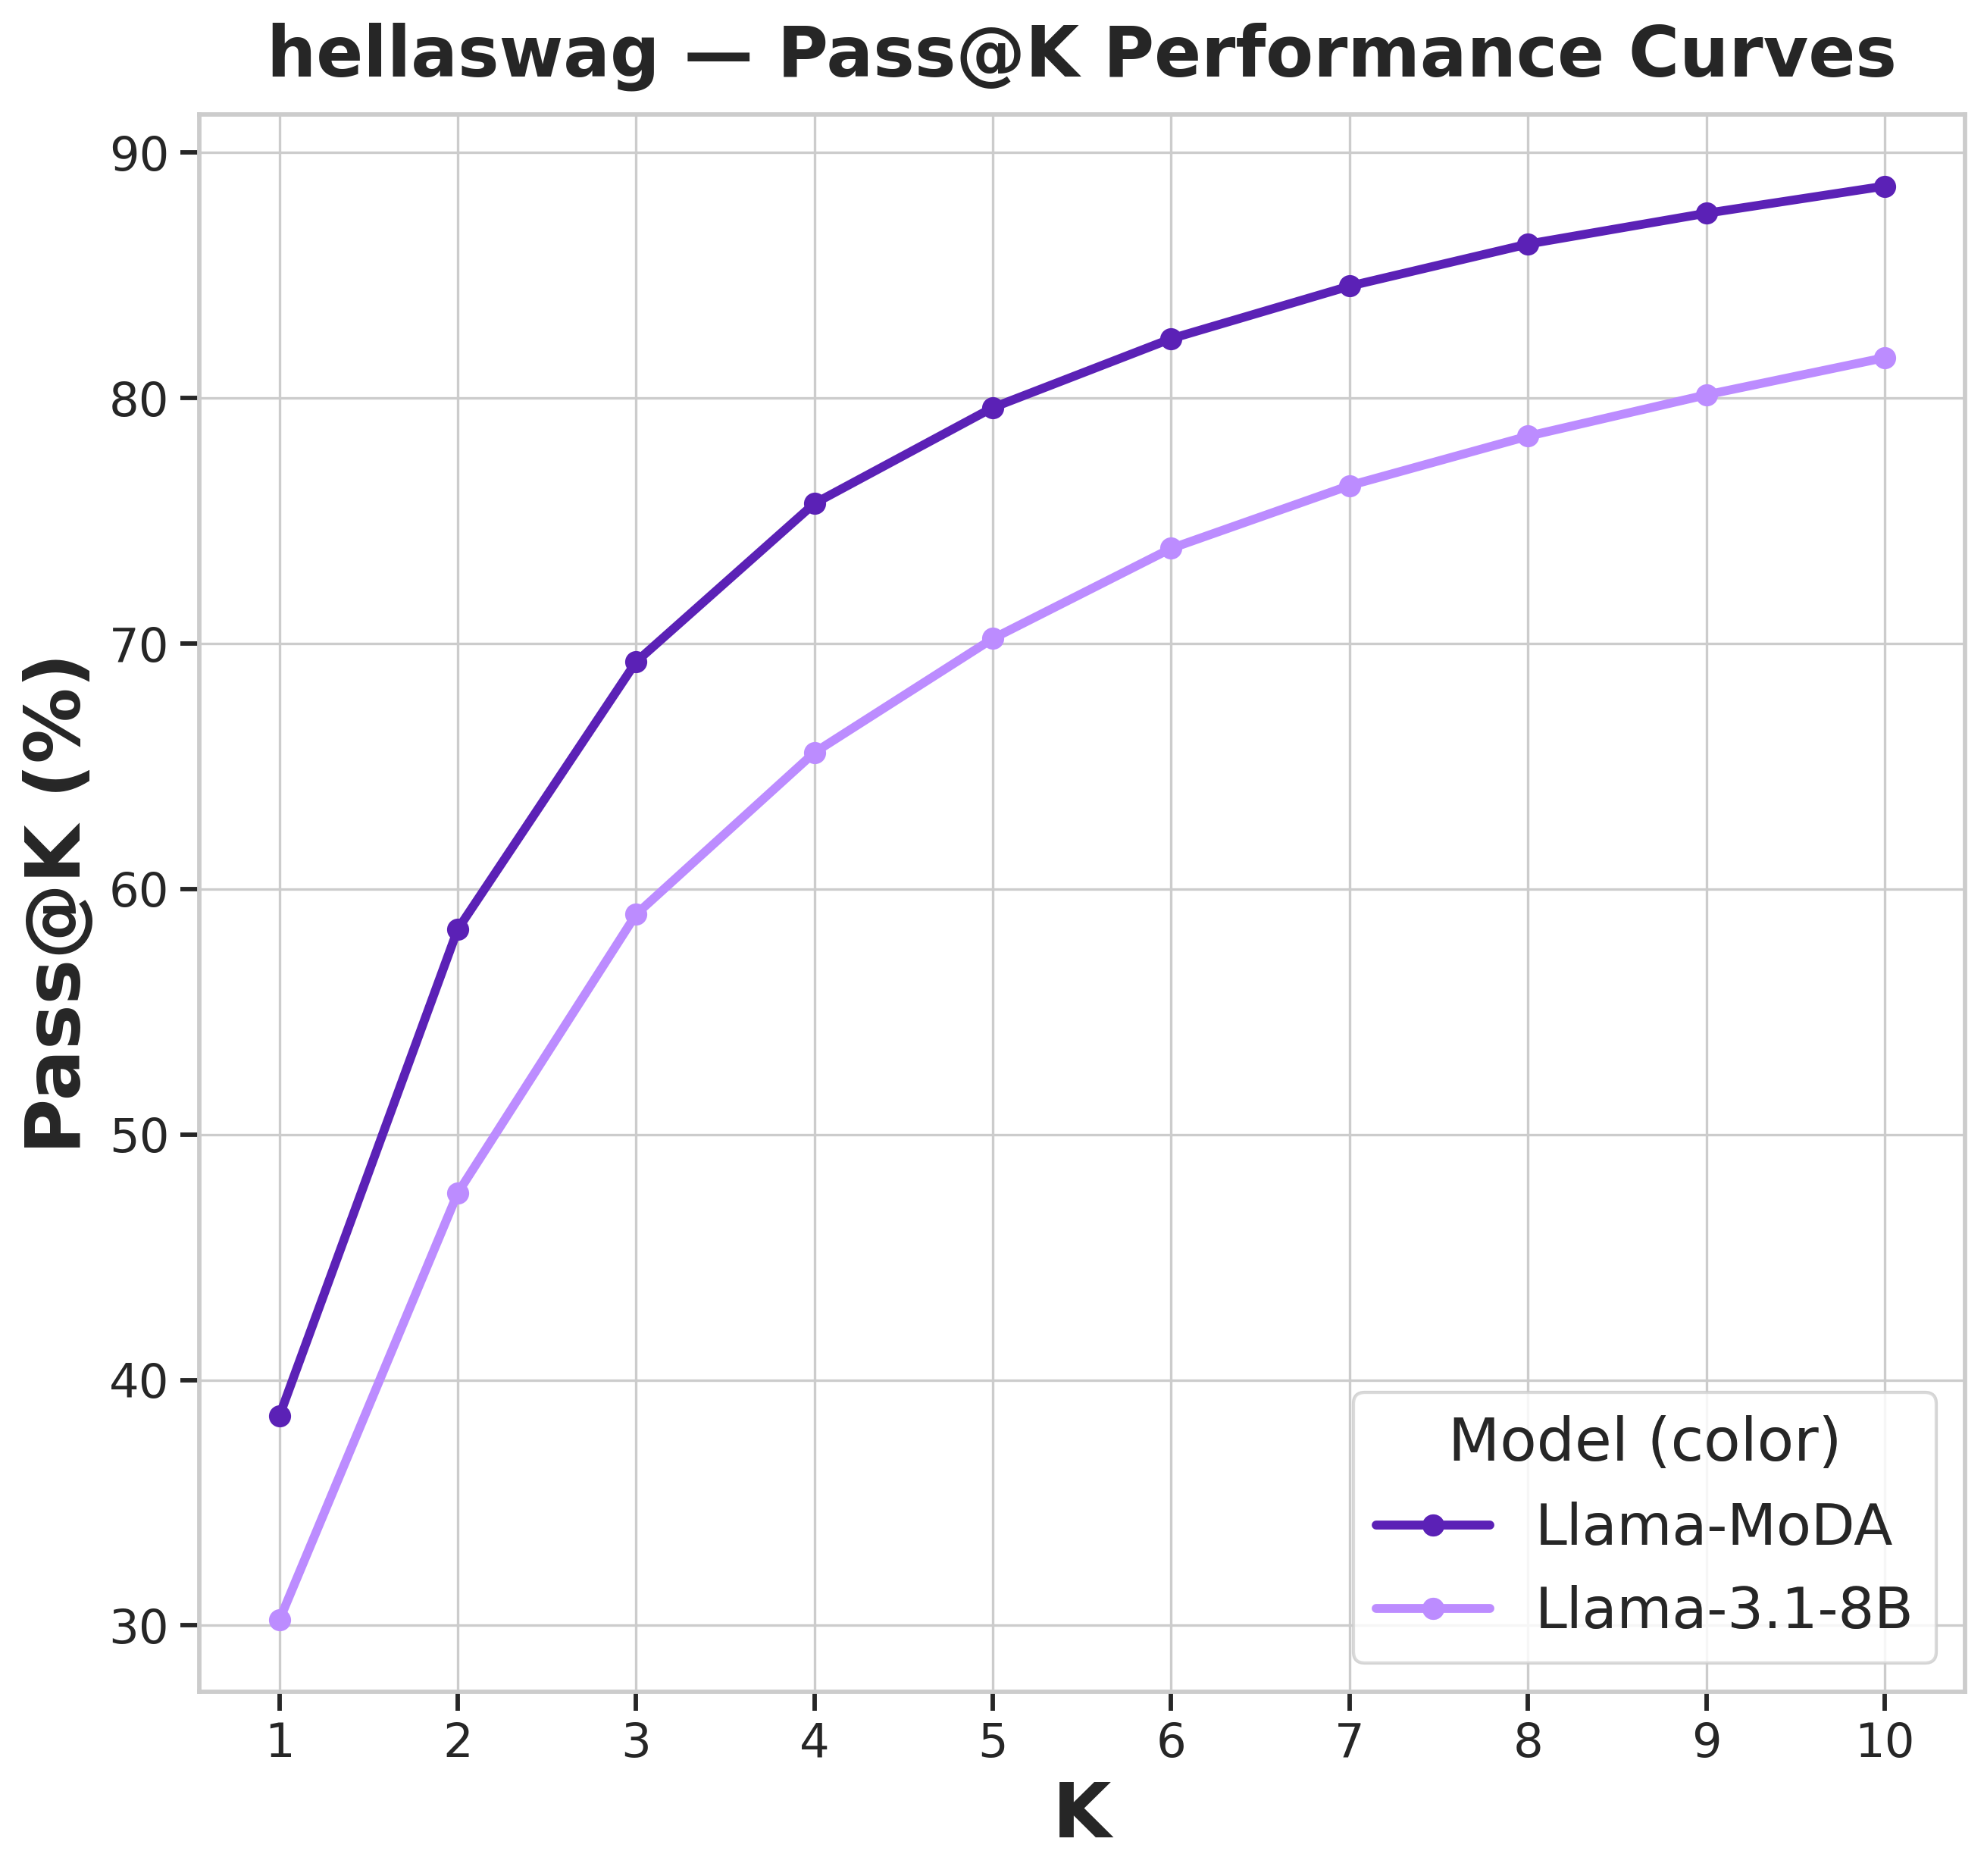
\includegraphics[width=\linewidth]{figures/main_pass_k/pass_at_k_figures/pass_at_k_hellaswag_thinking_false_base_model_llama3_1-8b.png}
\end{minipage}
\centering
\begin{minipage}{0.24\textwidth}
  \centering
  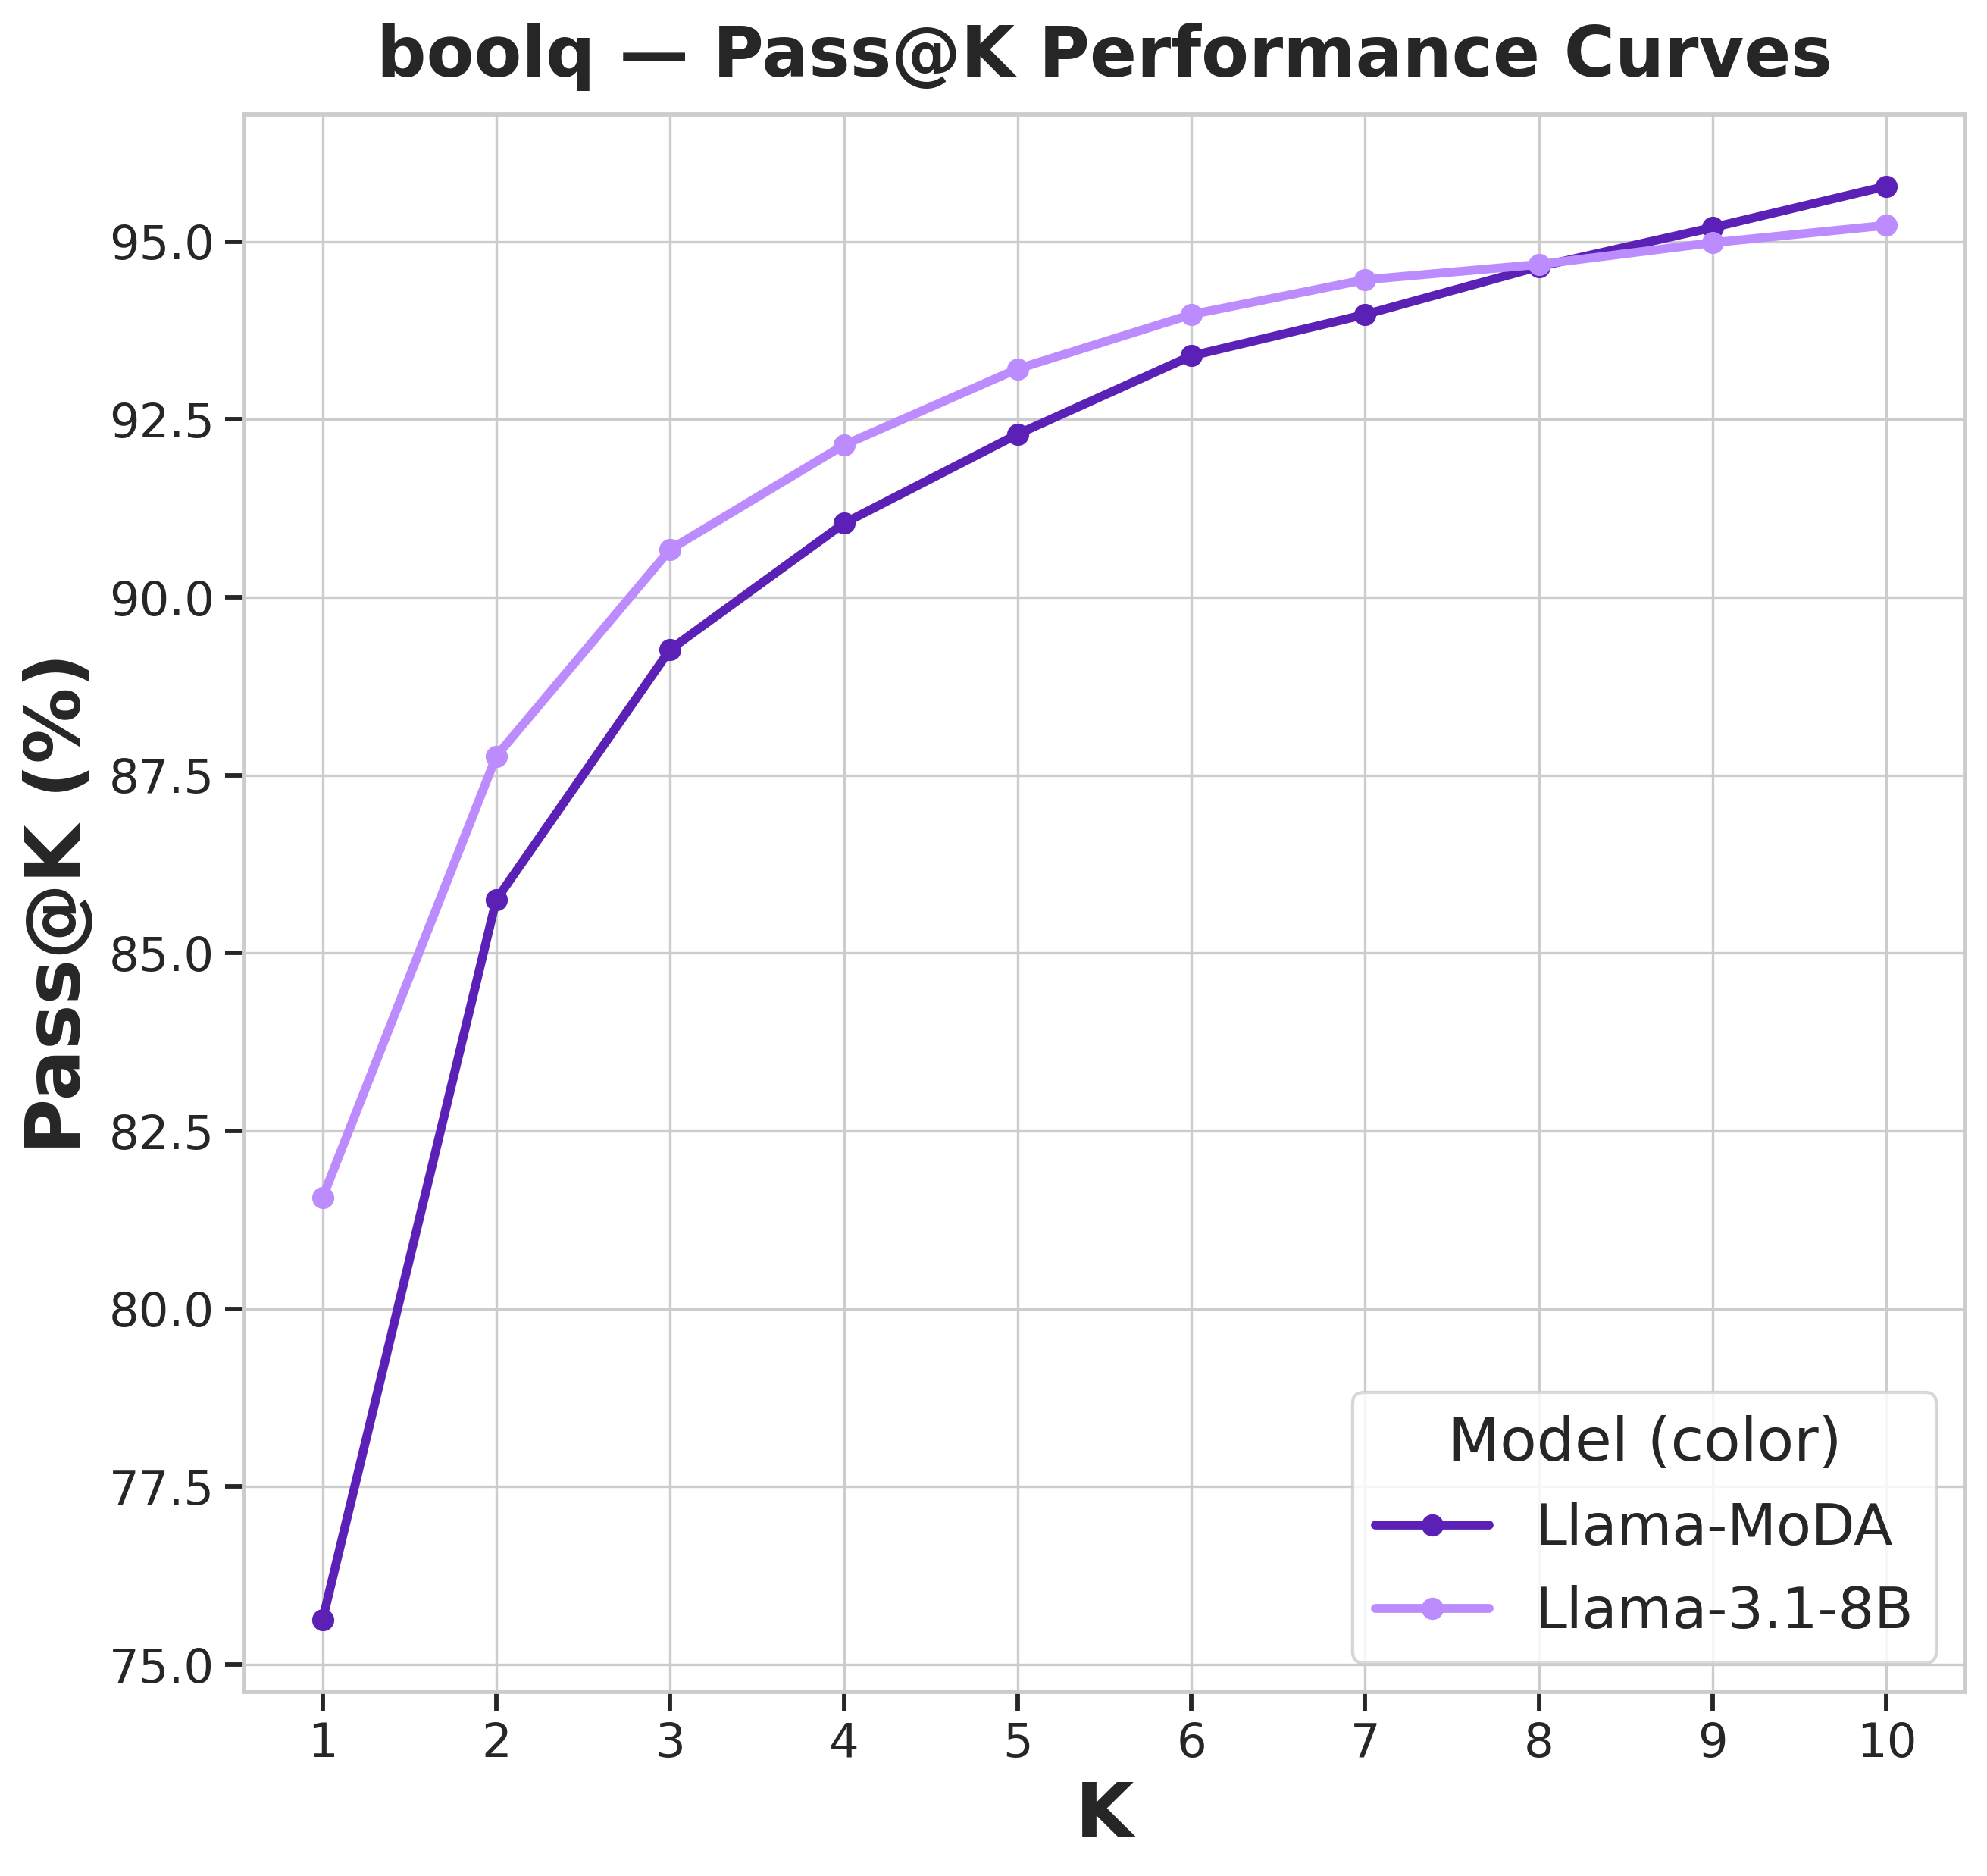
\includegraphics[width=\linewidth]{figures/main_pass_k/pass_at_k_figures/pass_at_k_boolq_thinking_false_base_model_llama3_1-8b.png}
\end{minipage}\hfill
\centering
\begin{minipage}{0.24\textwidth}
  \centering
  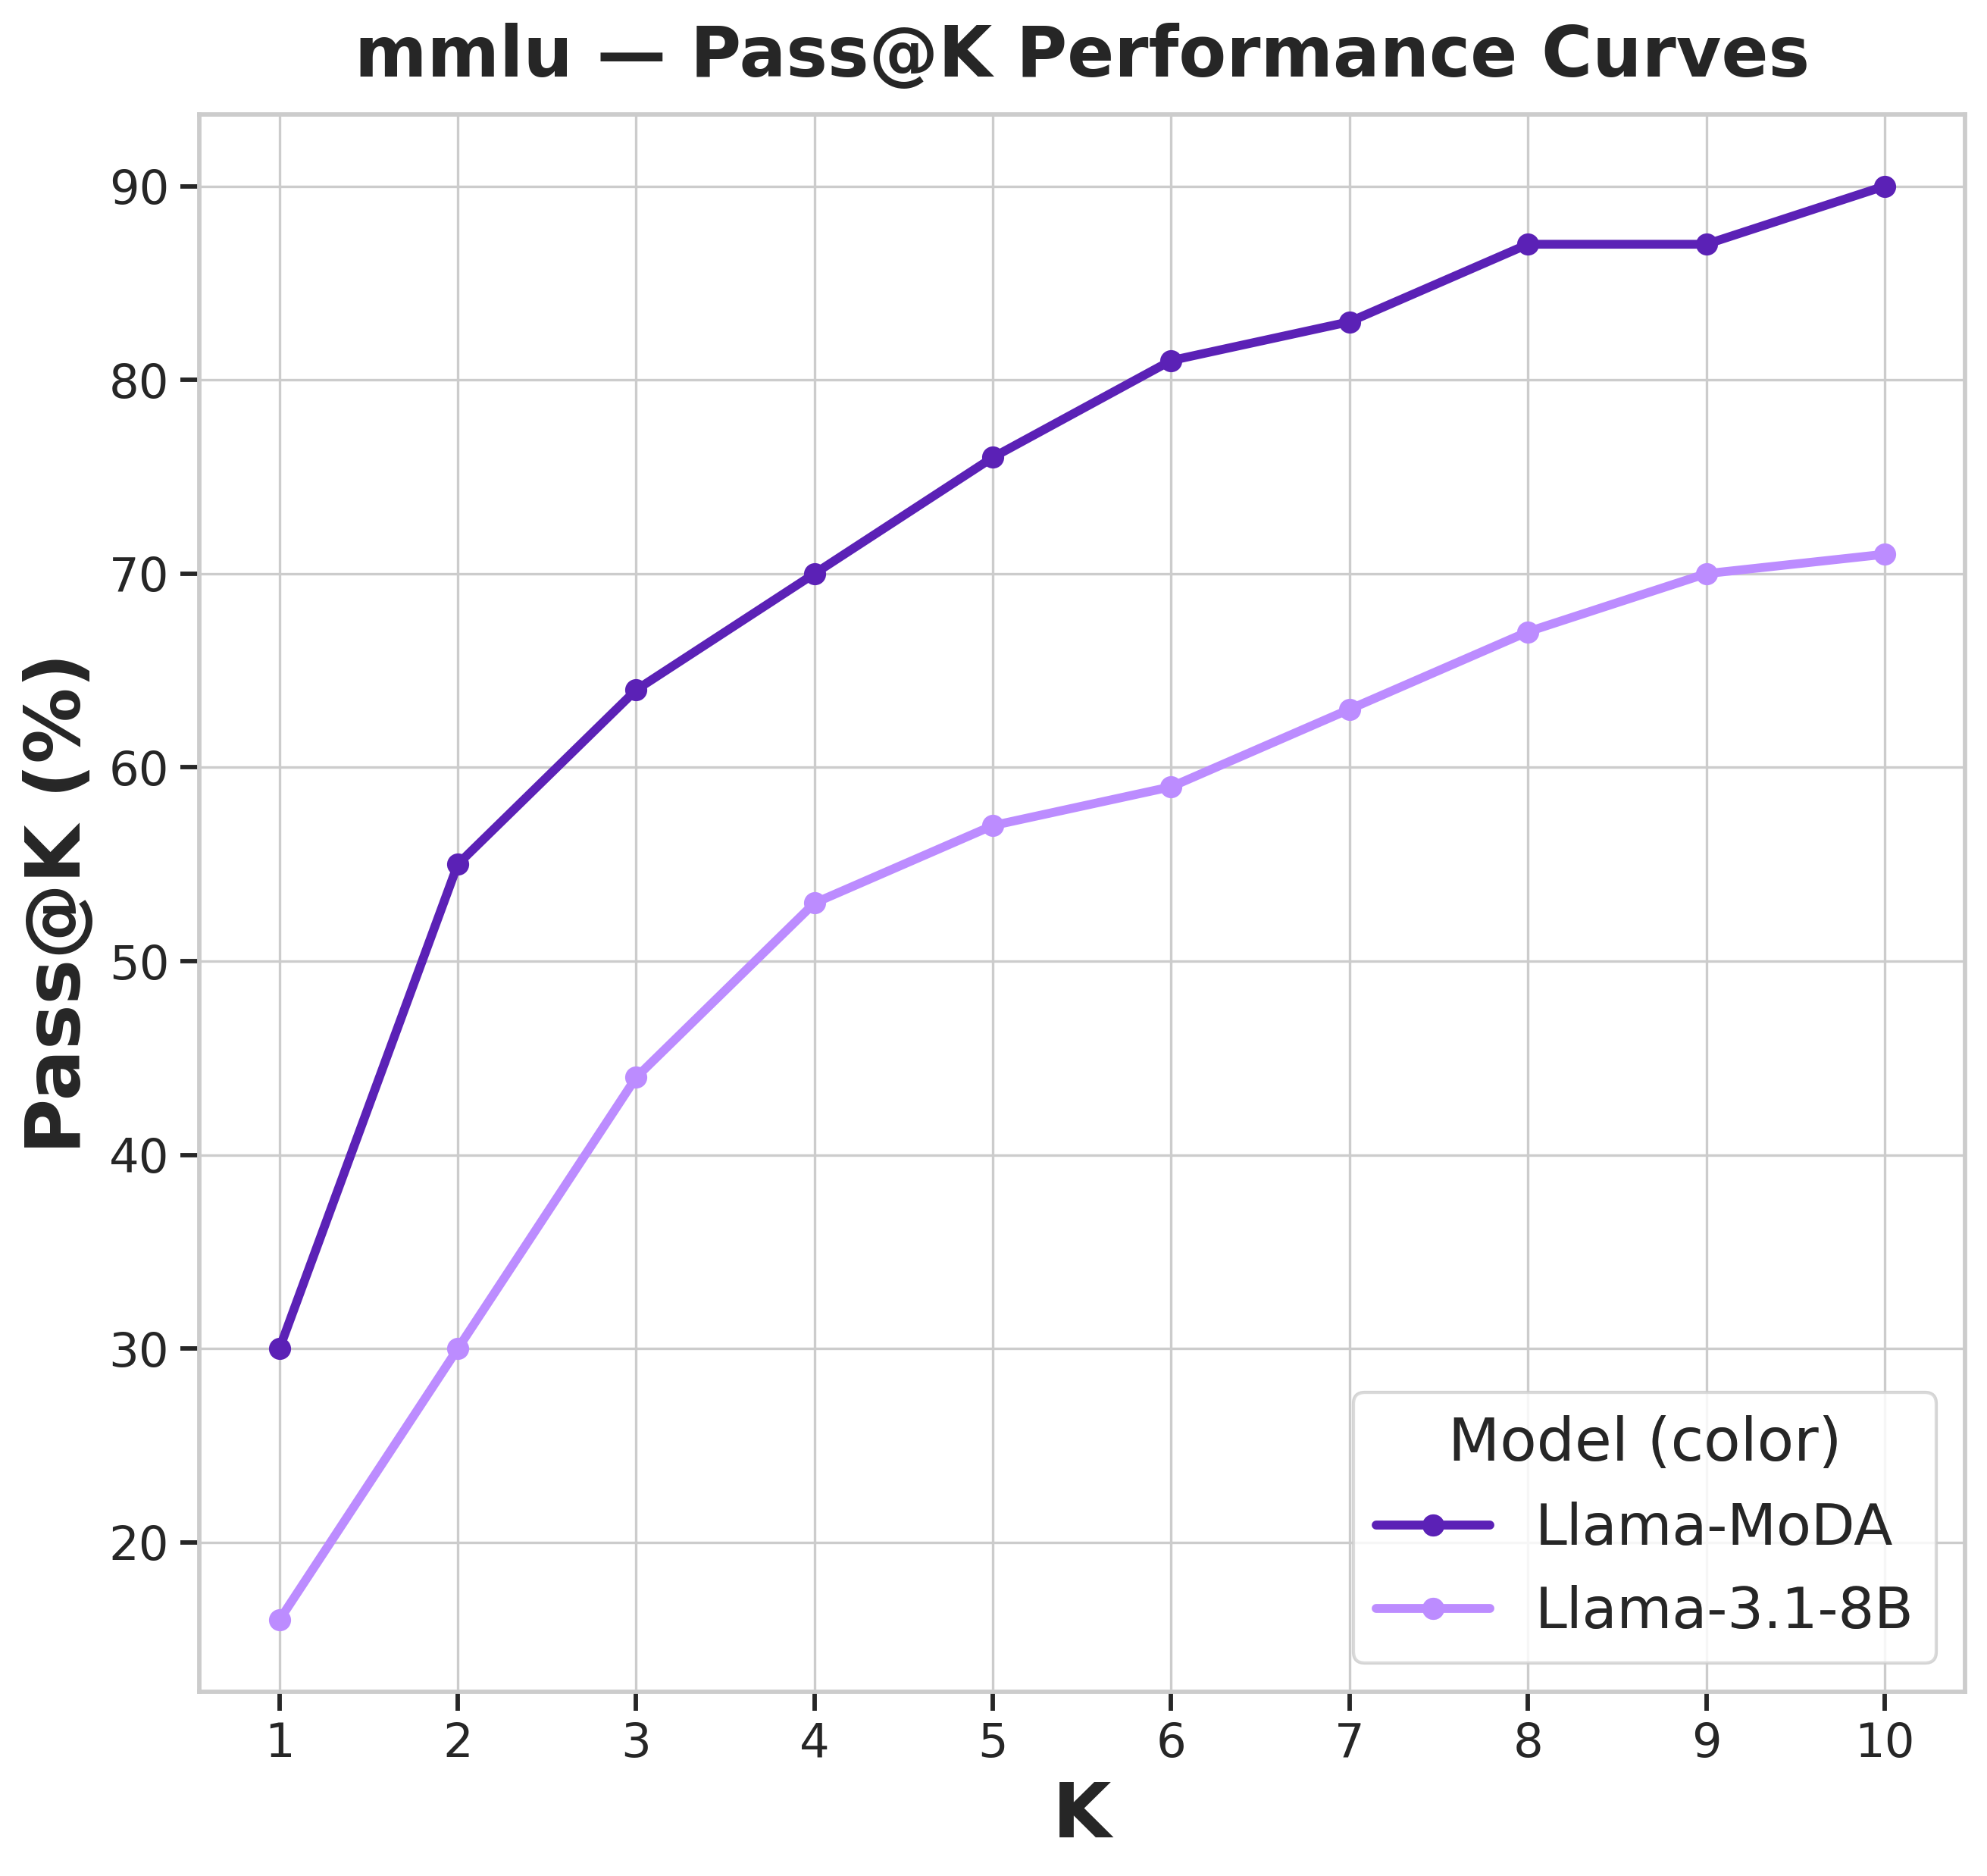
\includegraphics[width=\linewidth]{figures/main_pass_k/pass_at_k_figures/pass_at_k_mmlu_thinking_false_base_model_llama3_1-8b.png}
\end{minipage}\hfill
\begin{minipage}{0.24\textwidth}
  \centering
  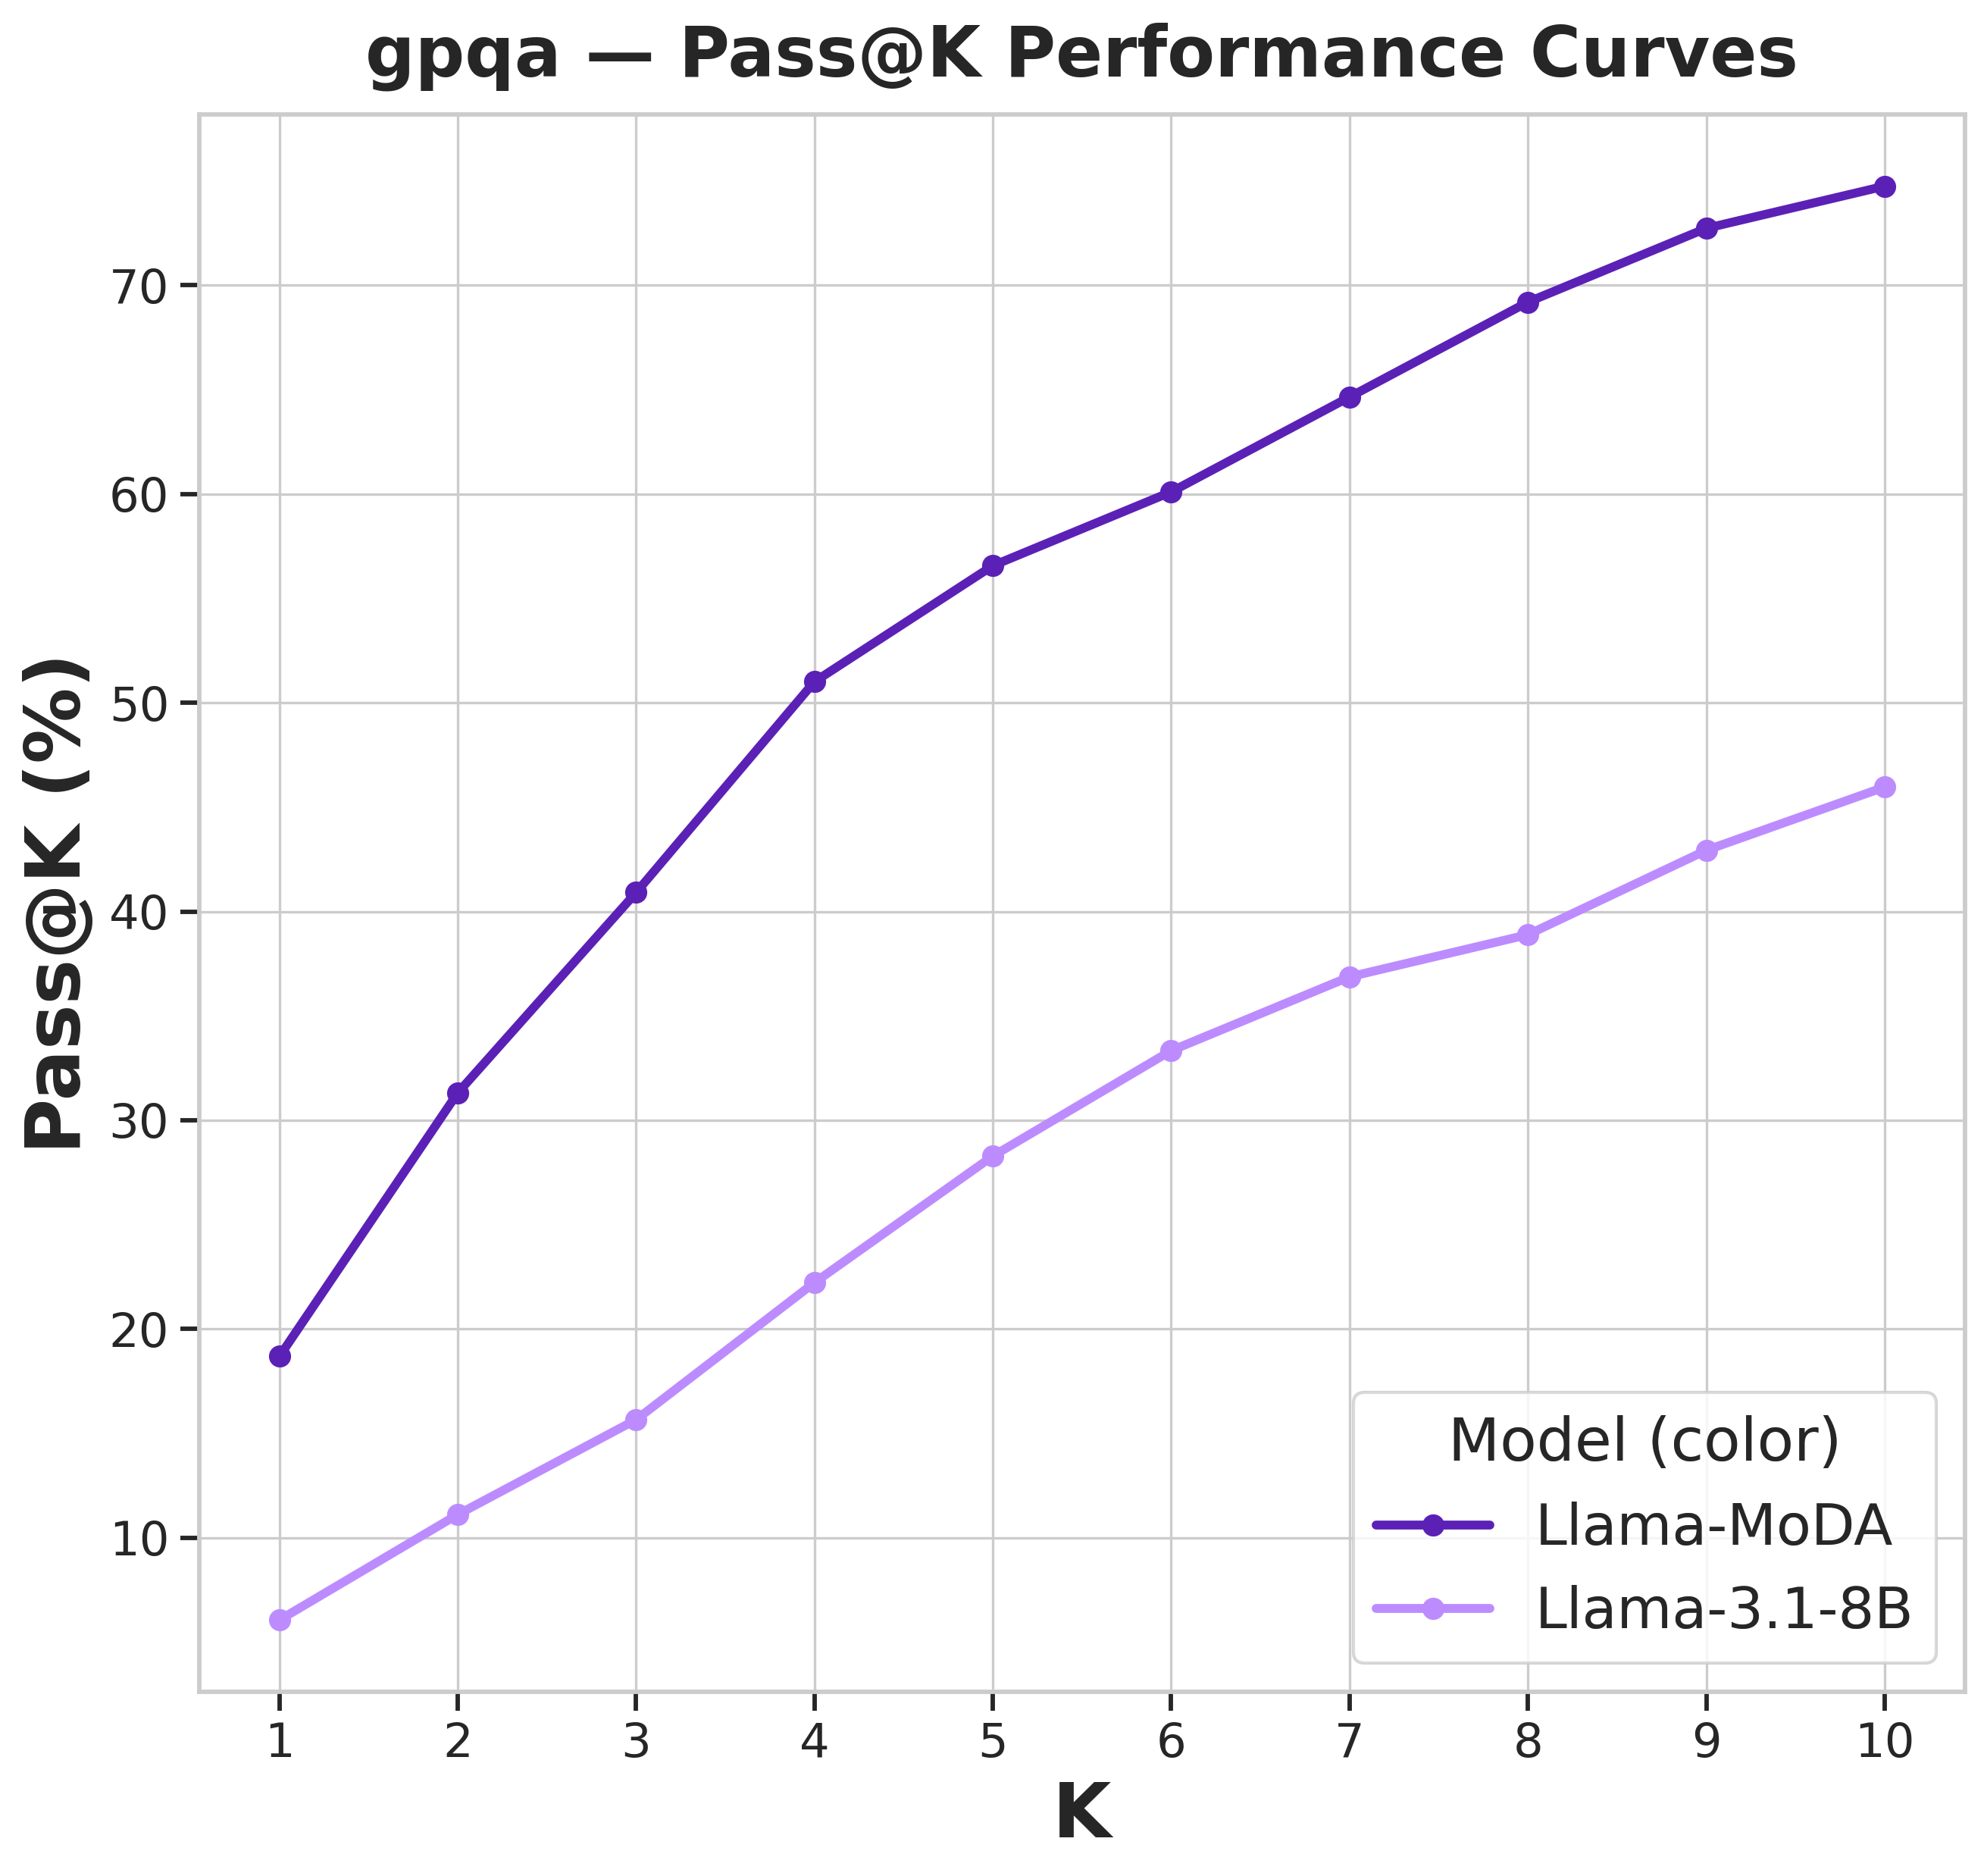
\includegraphics[width=\linewidth]{figures/main_pass_k/pass_at_k_figures/pass_at_k_gpqa_thinking_false_base_model_llama3_1-8b.png}
\end{minipage}\hfill
\begin{minipage}{0.24\textwidth}
  \centering
  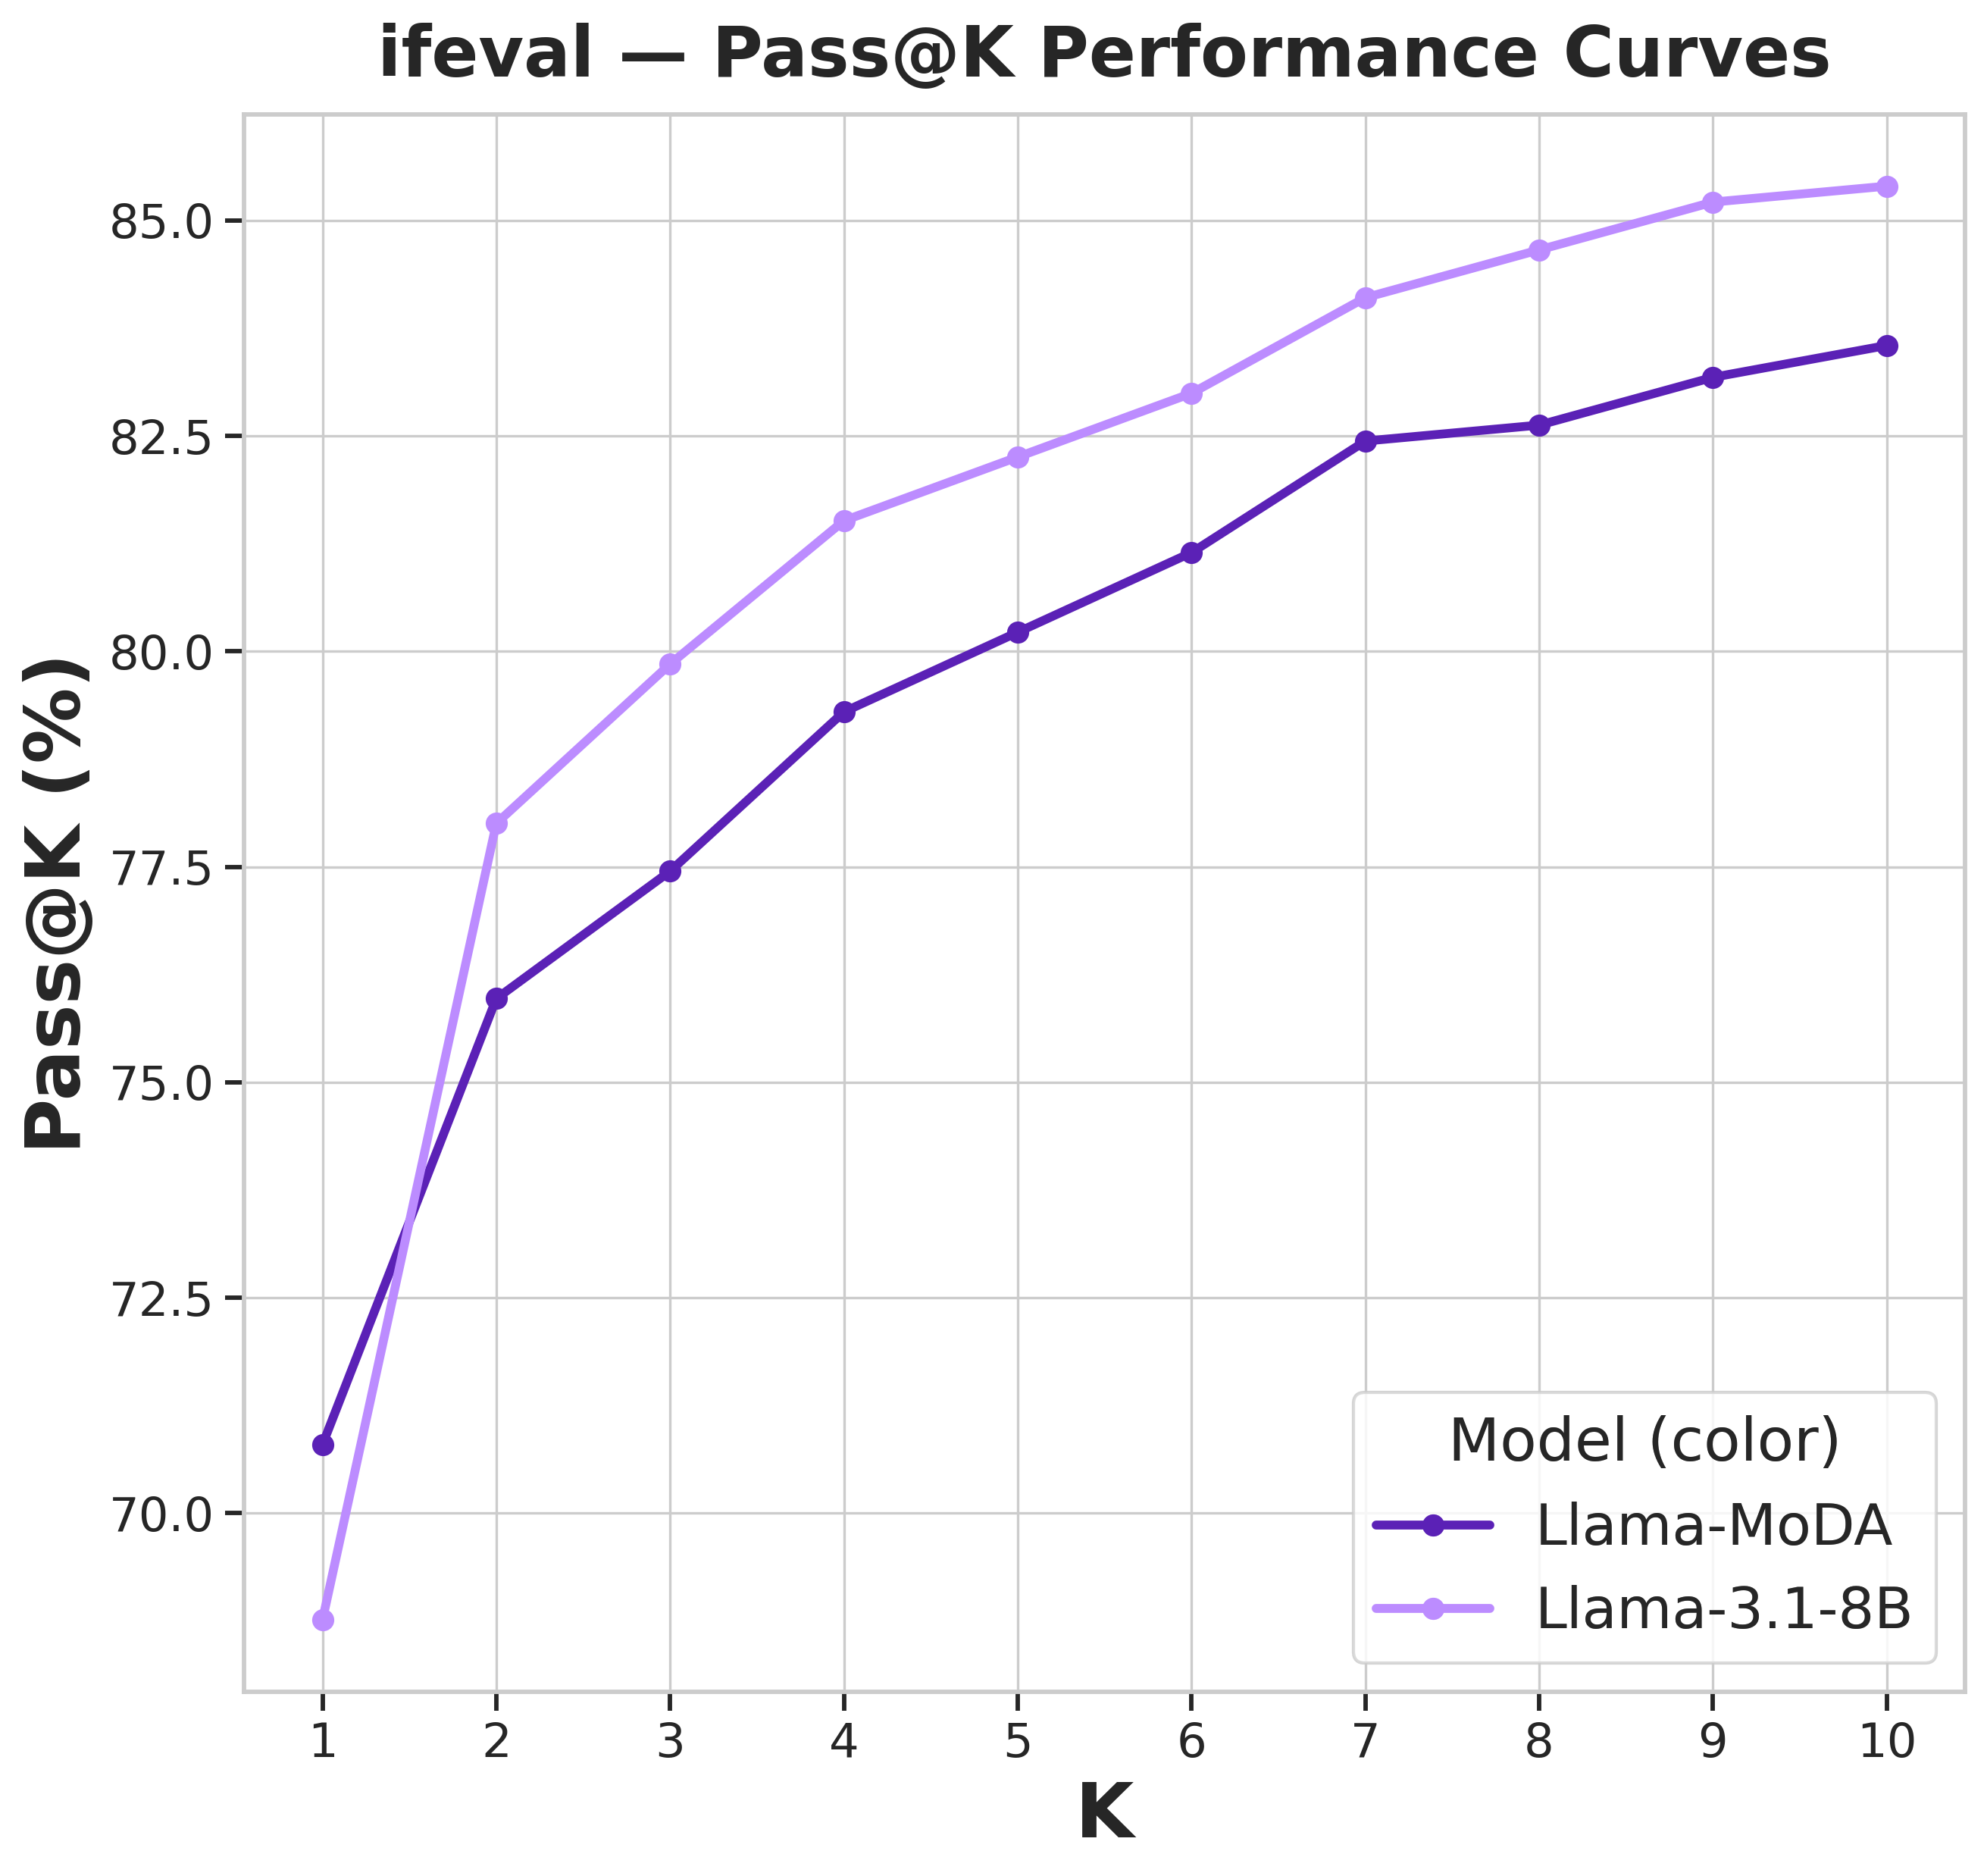
\includegraphics[width=\linewidth]{figures/main_pass_k/pass_at_k_figures/pass_at_k_ifeval_thinking_false_base_model_llama3_1-8b.png}
\end{minipage}
\caption{\textbf{General capability retention: pass@k accuracy.} Llama-3.1-8B base and thinking disabled models.}
\label{fig:general capability pass@k llama}
\end{figure}



\begin{figure}[H]
\begin{minipage}{0.24\textwidth}
  \centering
  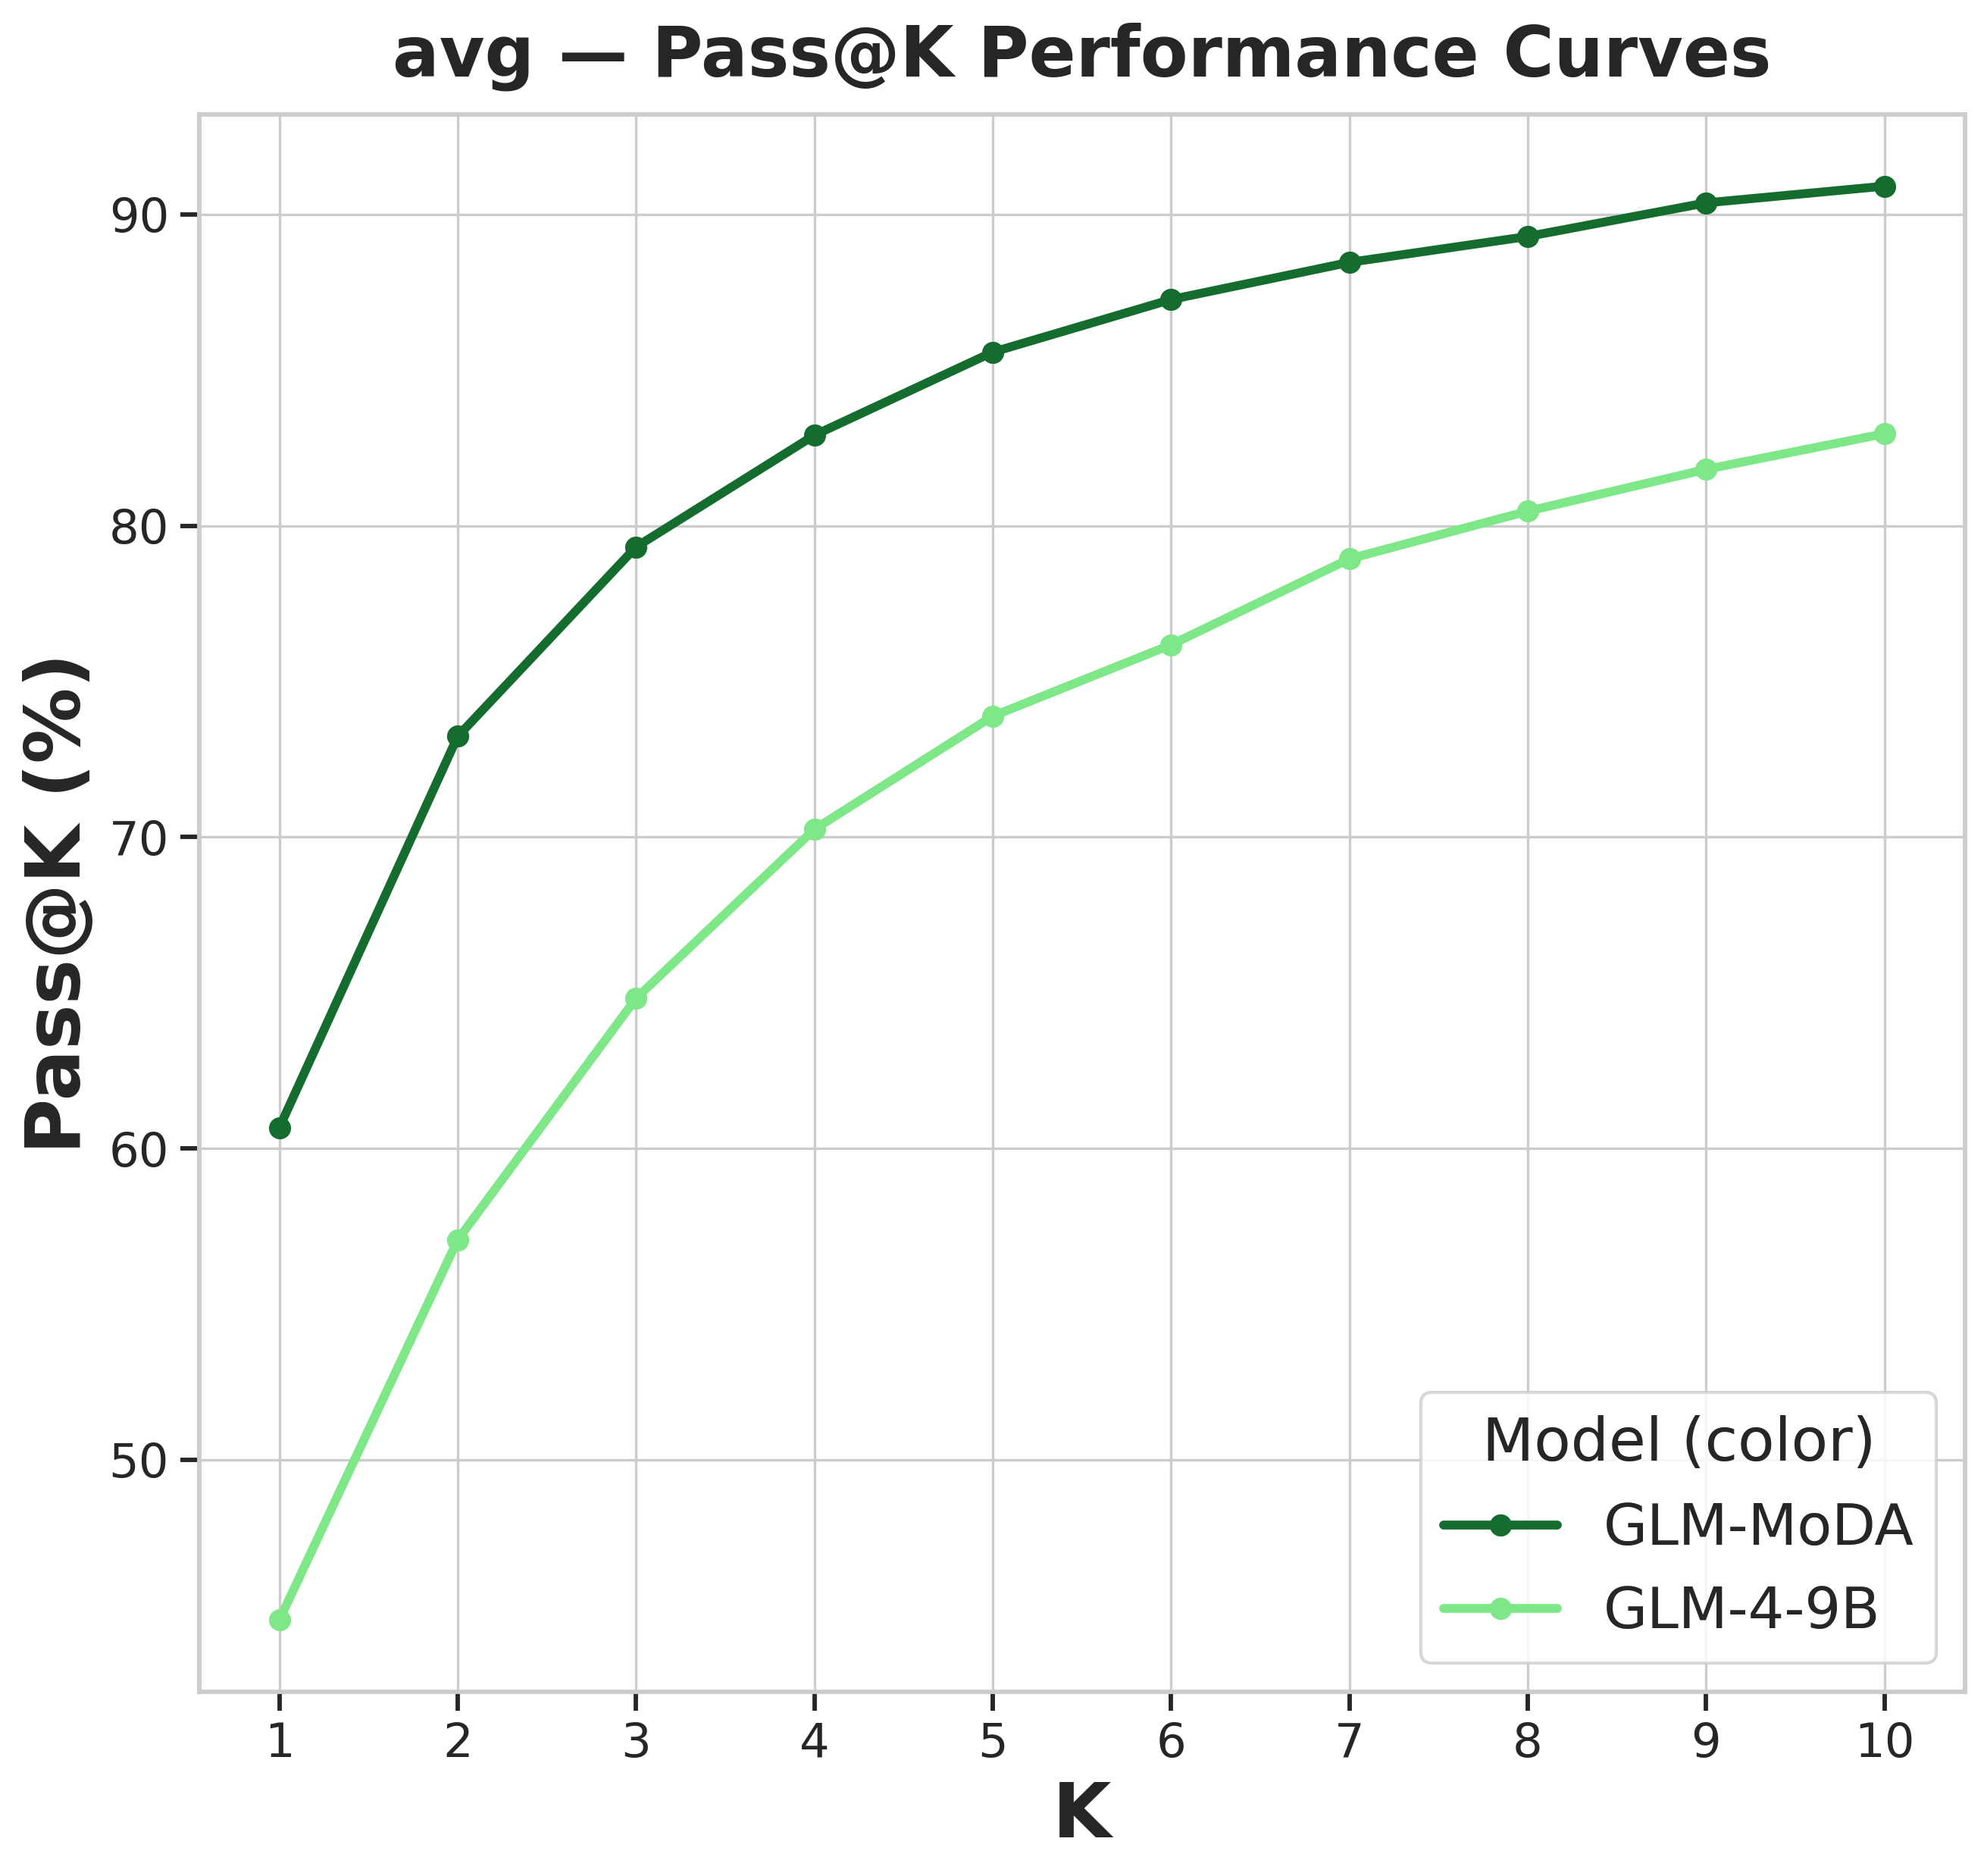
\includegraphics[width=\linewidth]{figures/main_pass_k/pass_at_k_figures/pass_at_k_avg_thinking_false_base_model_glm-4-9b.png}
\end{minipage}\hfill
\centering
\begin{minipage}{0.24\textwidth}
  \centering
  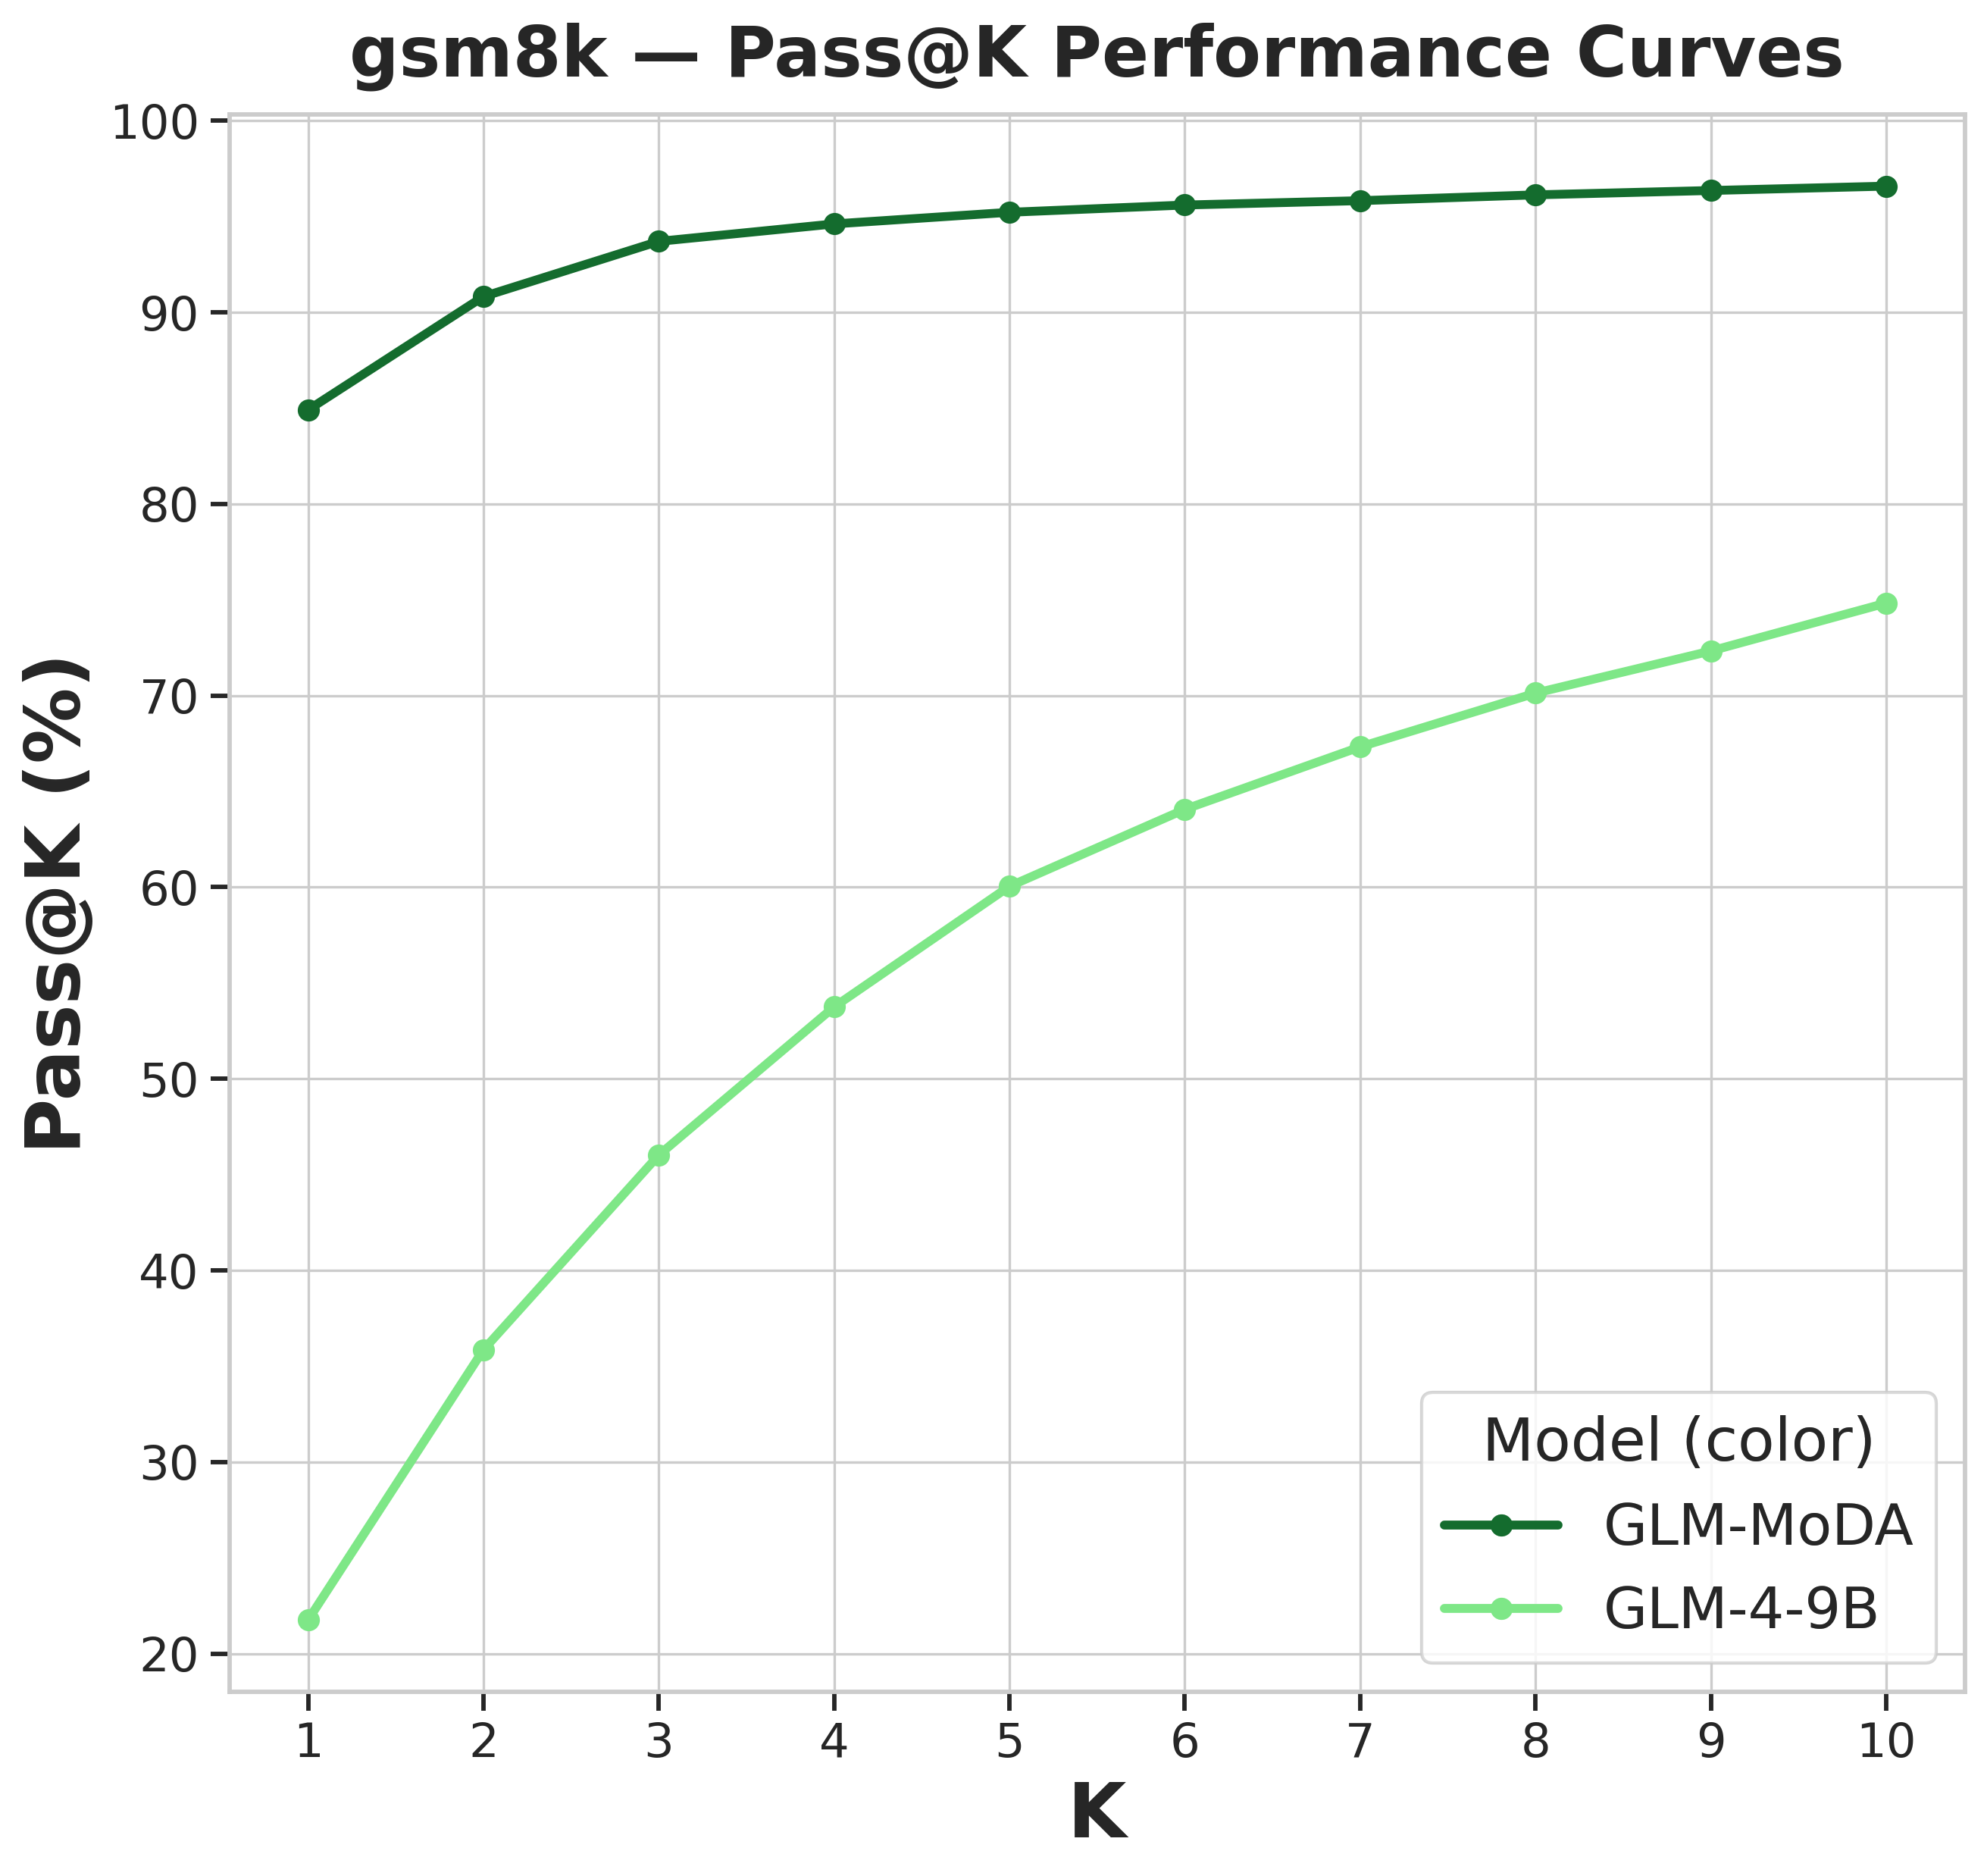
\includegraphics[width=\linewidth]{figures/main_pass_k/pass_at_k_figures/pass_at_k_gsm8k_thinking_false_base_model_glm-4-9b.png}
\end{minipage}\hfill
\begin{minipage}{0.24\textwidth}
  \centering
  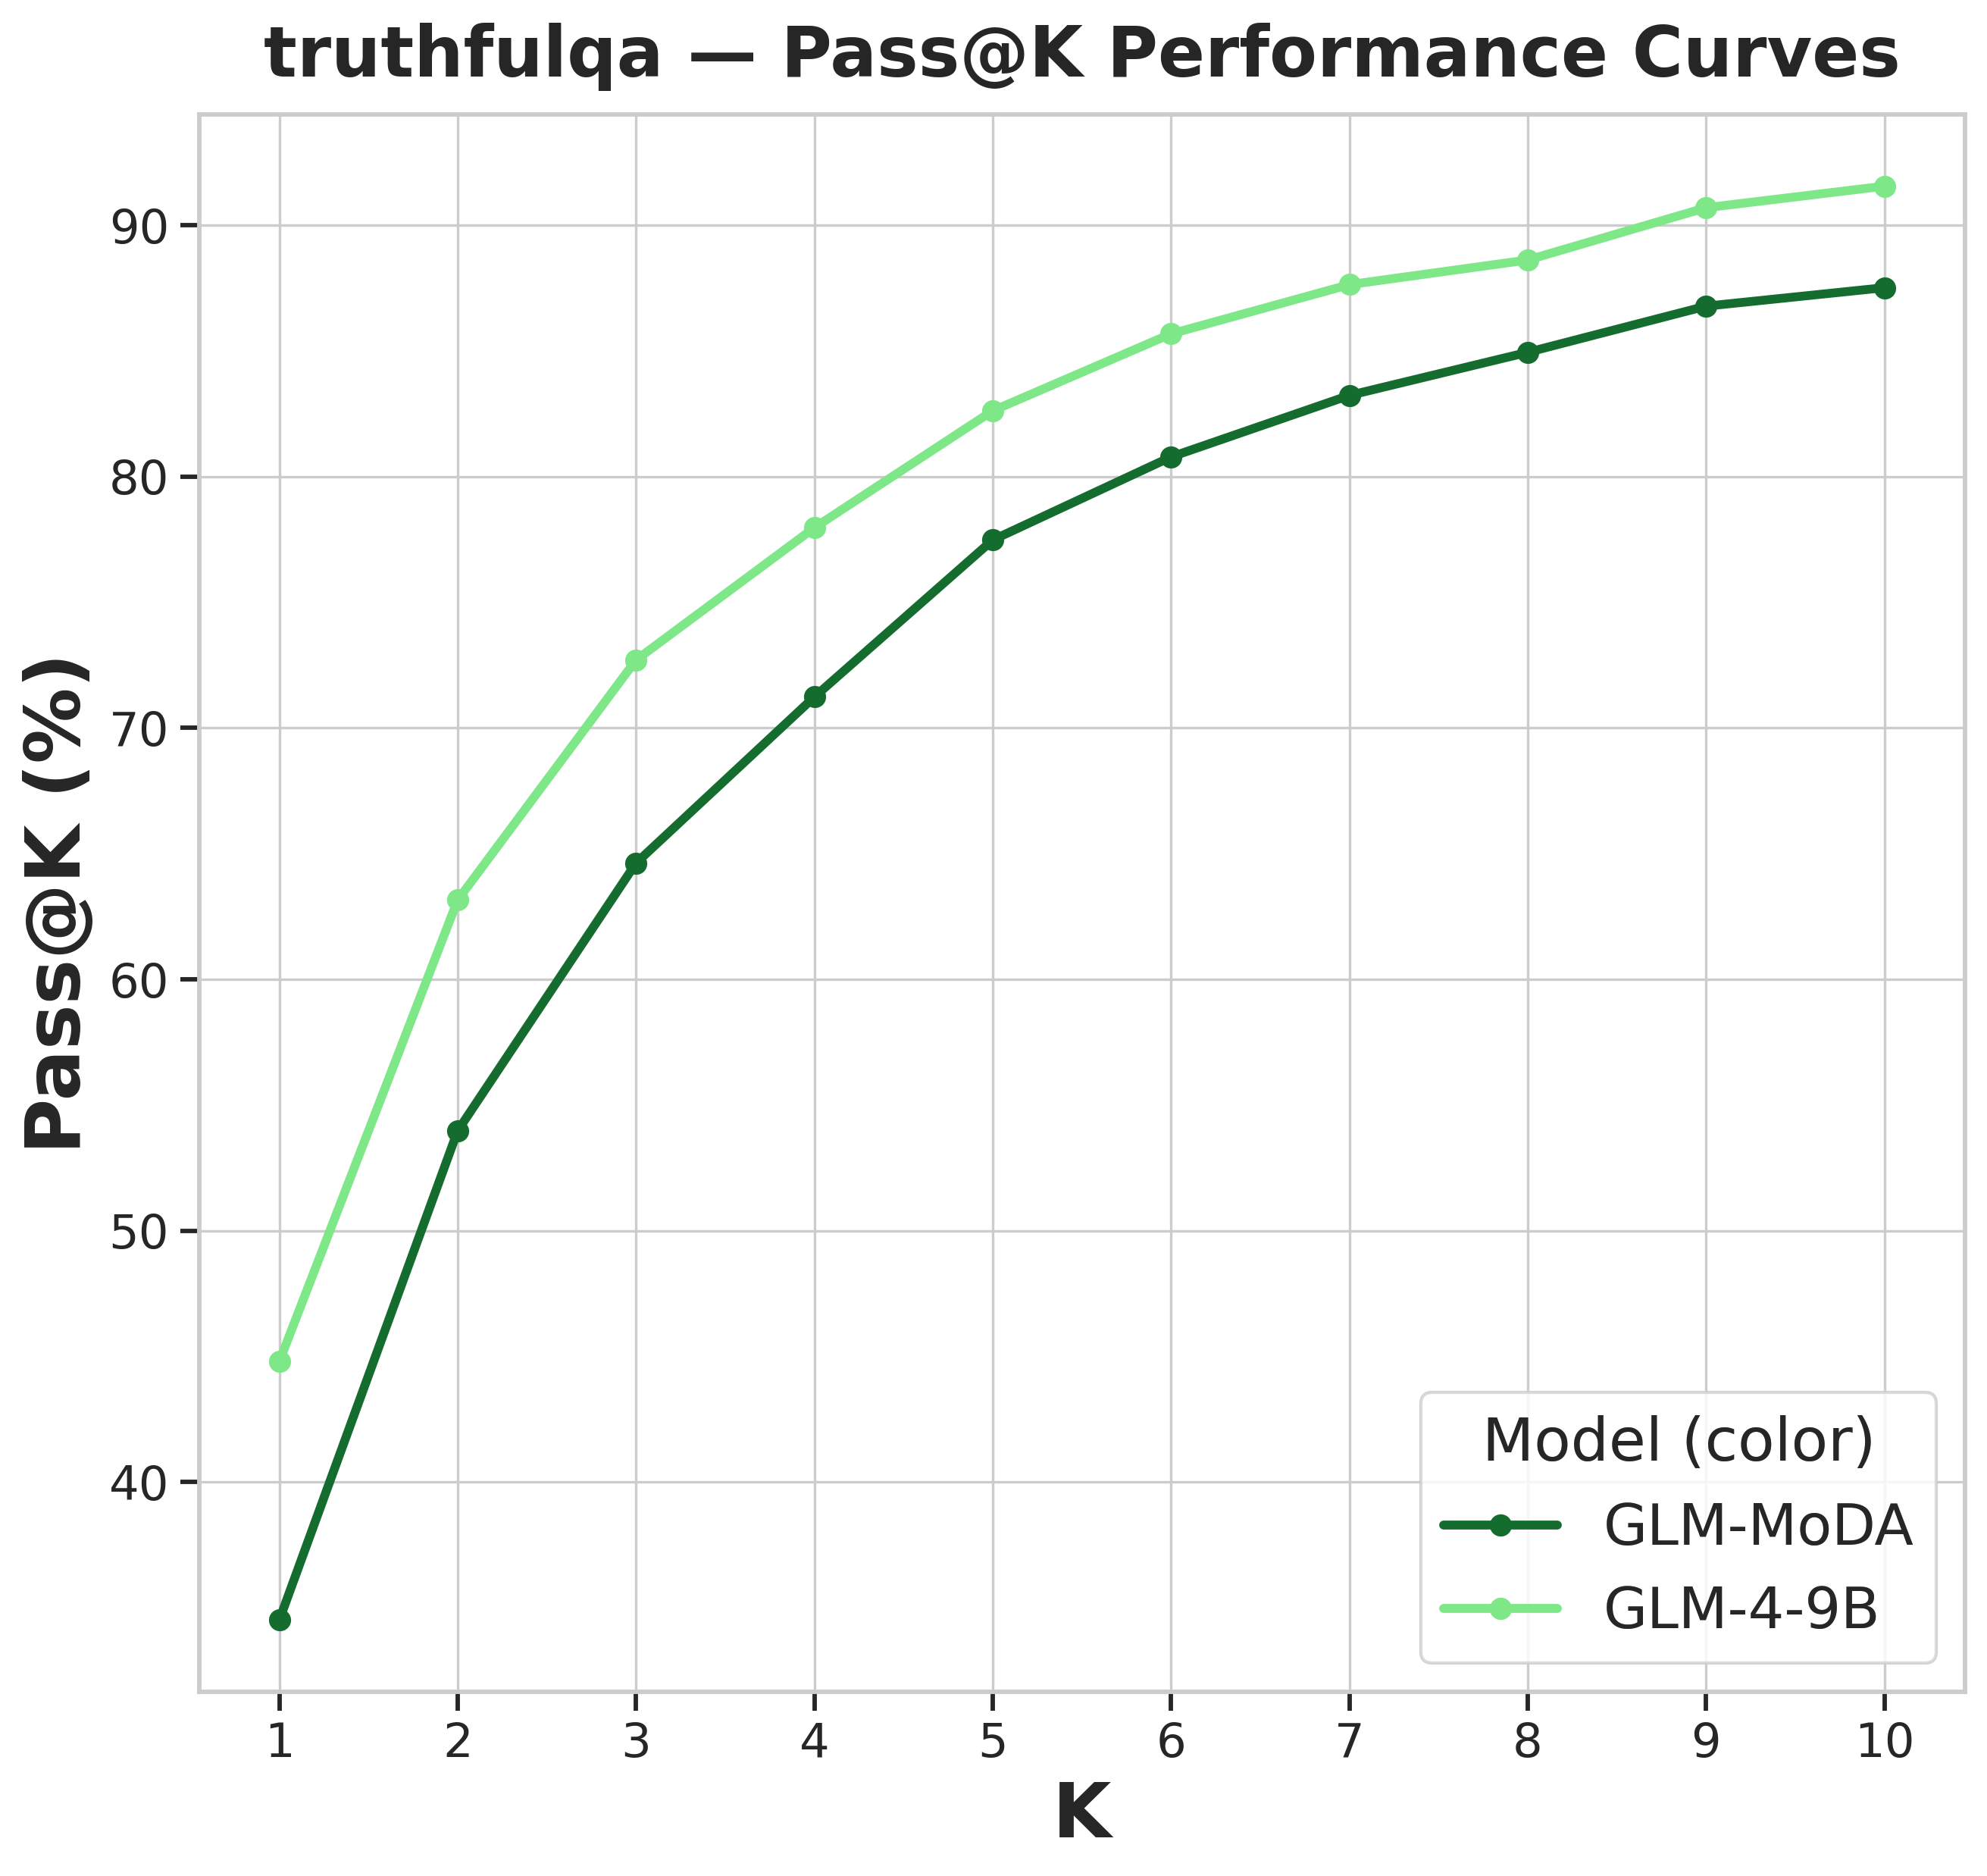
\includegraphics[width=\linewidth]{figures/main_pass_k/pass_at_k_figures/pass_at_k_truthfulqa_thinking_false_base_model_glm-4-9b.png}
\end{minipage}\hfill
\begin{minipage}{0.24\textwidth}
  \centering
  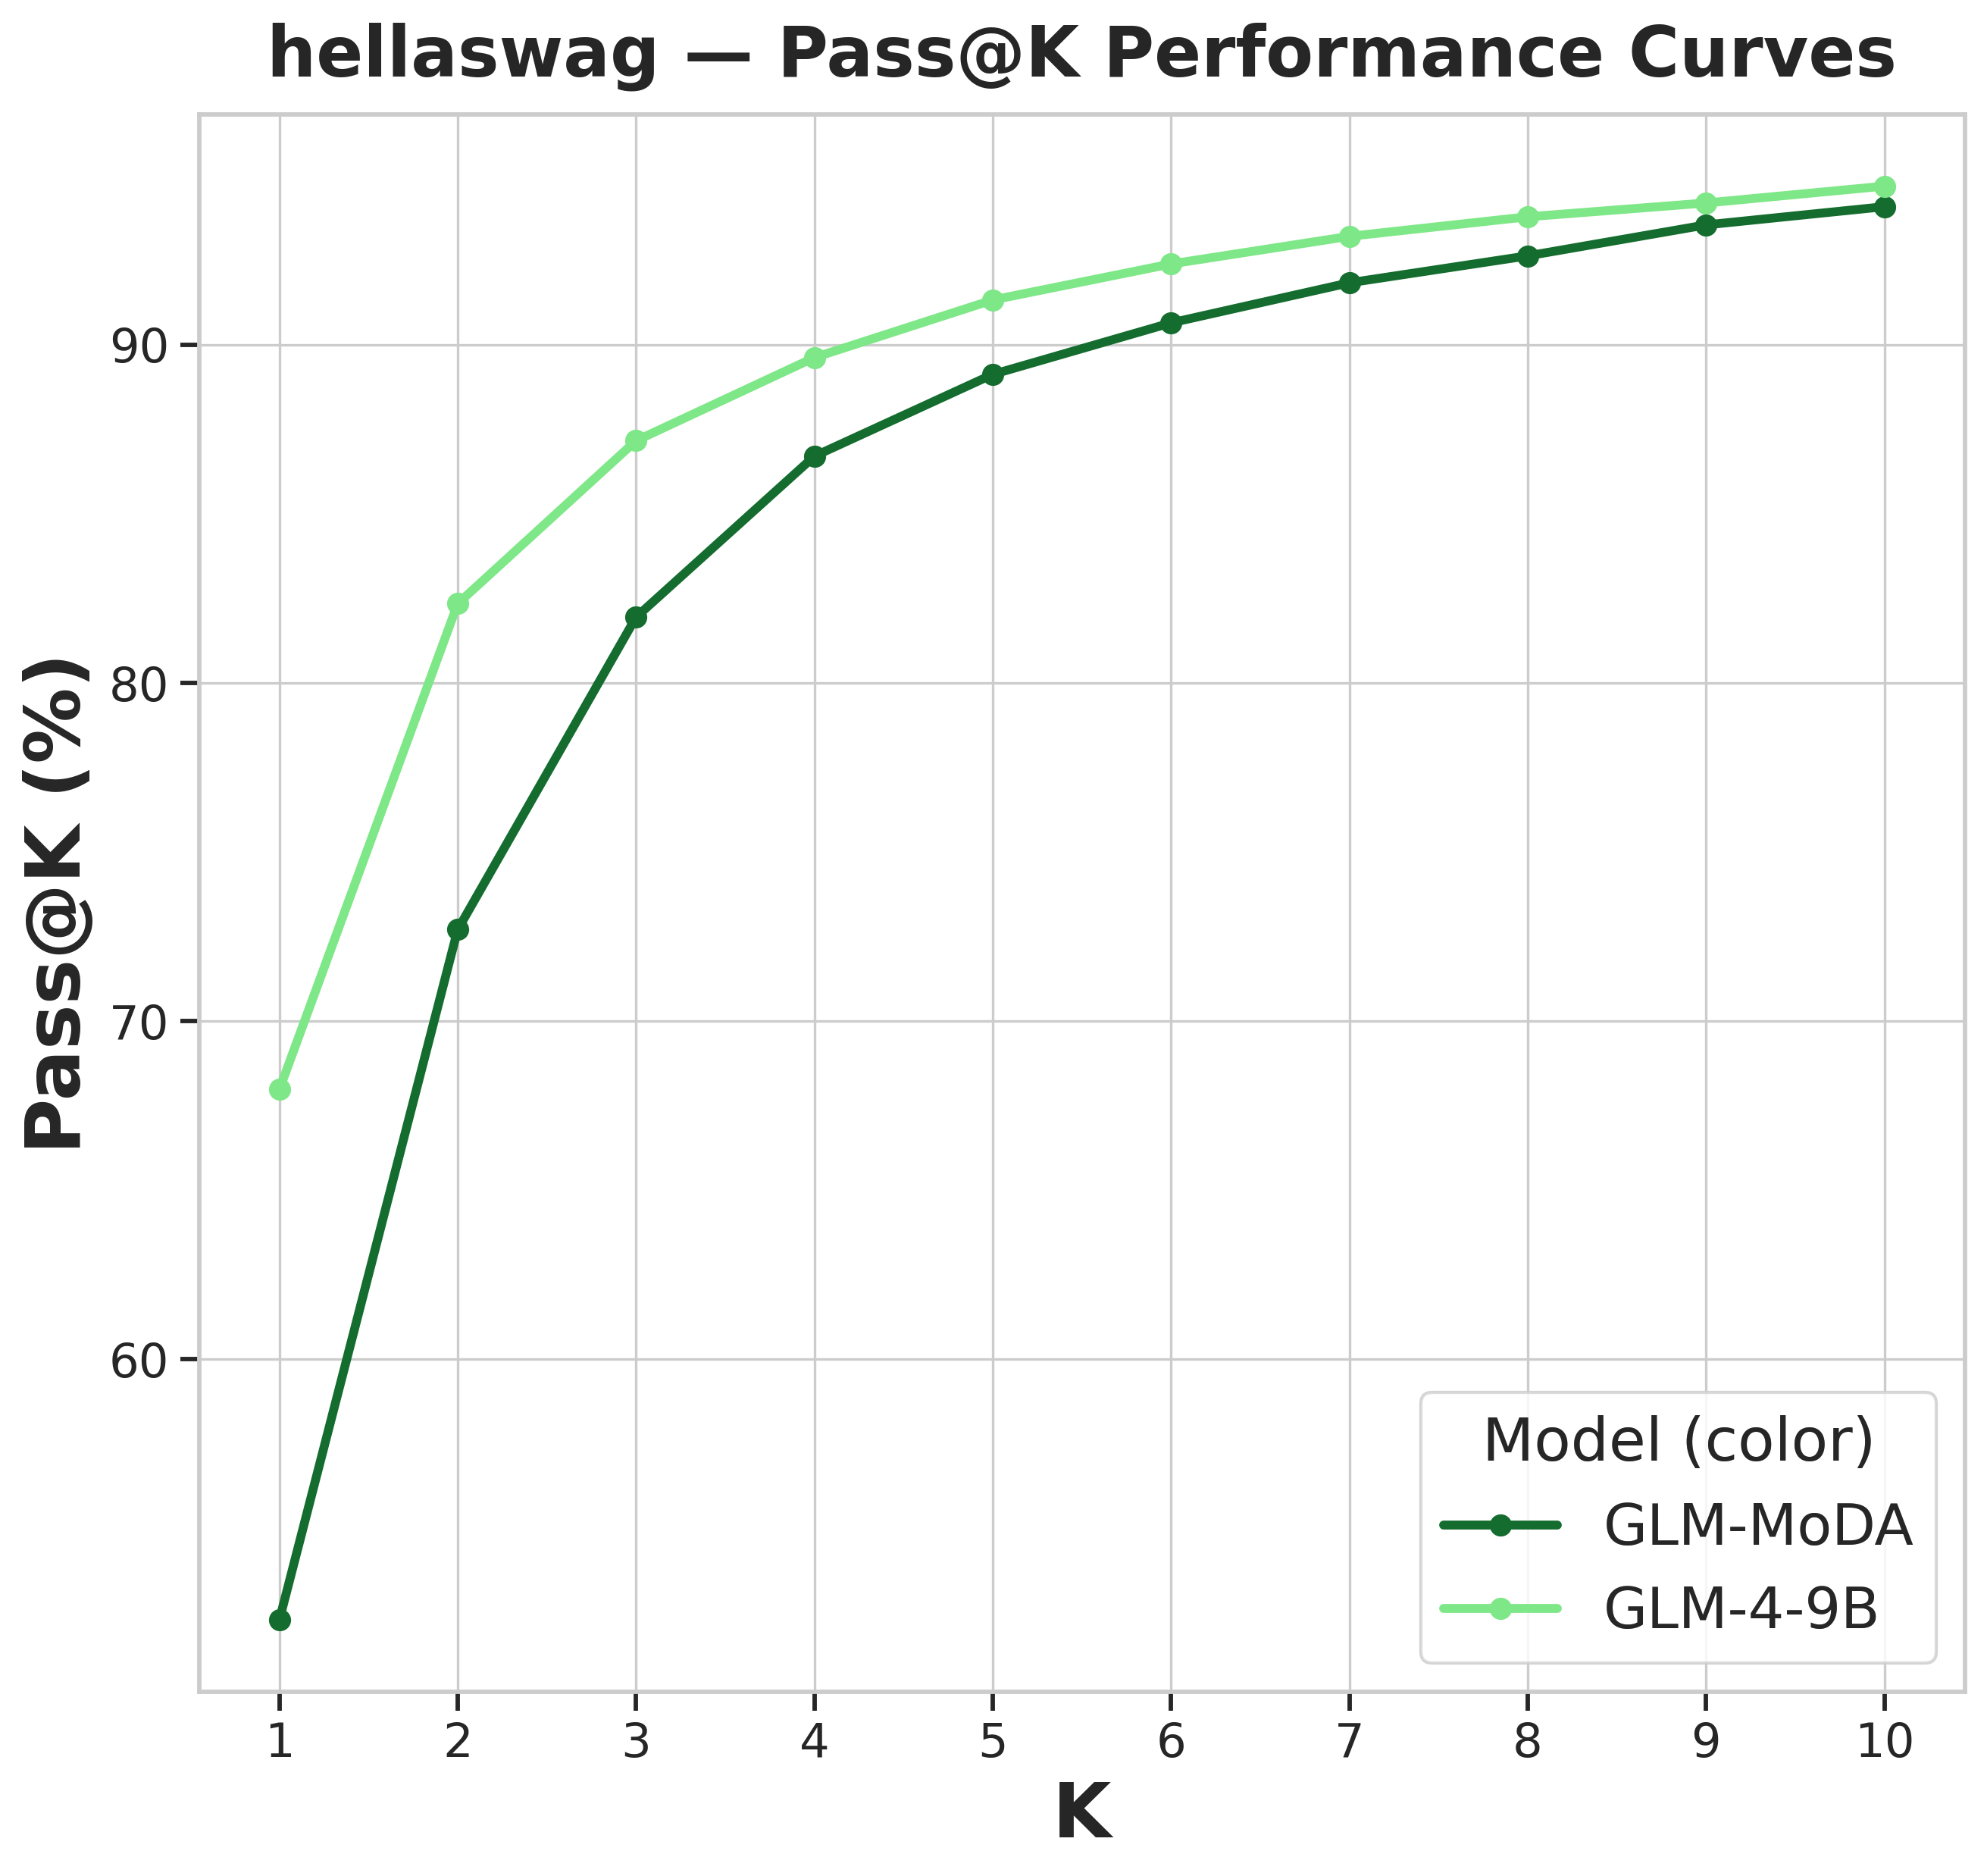
\includegraphics[width=\linewidth]{figures/main_pass_k/pass_at_k_figures/pass_at_k_hellaswag_thinking_false_base_model_glm-4-9b.png}
\end{minipage}
\centering
\begin{minipage}{0.24\textwidth}
  \centering
  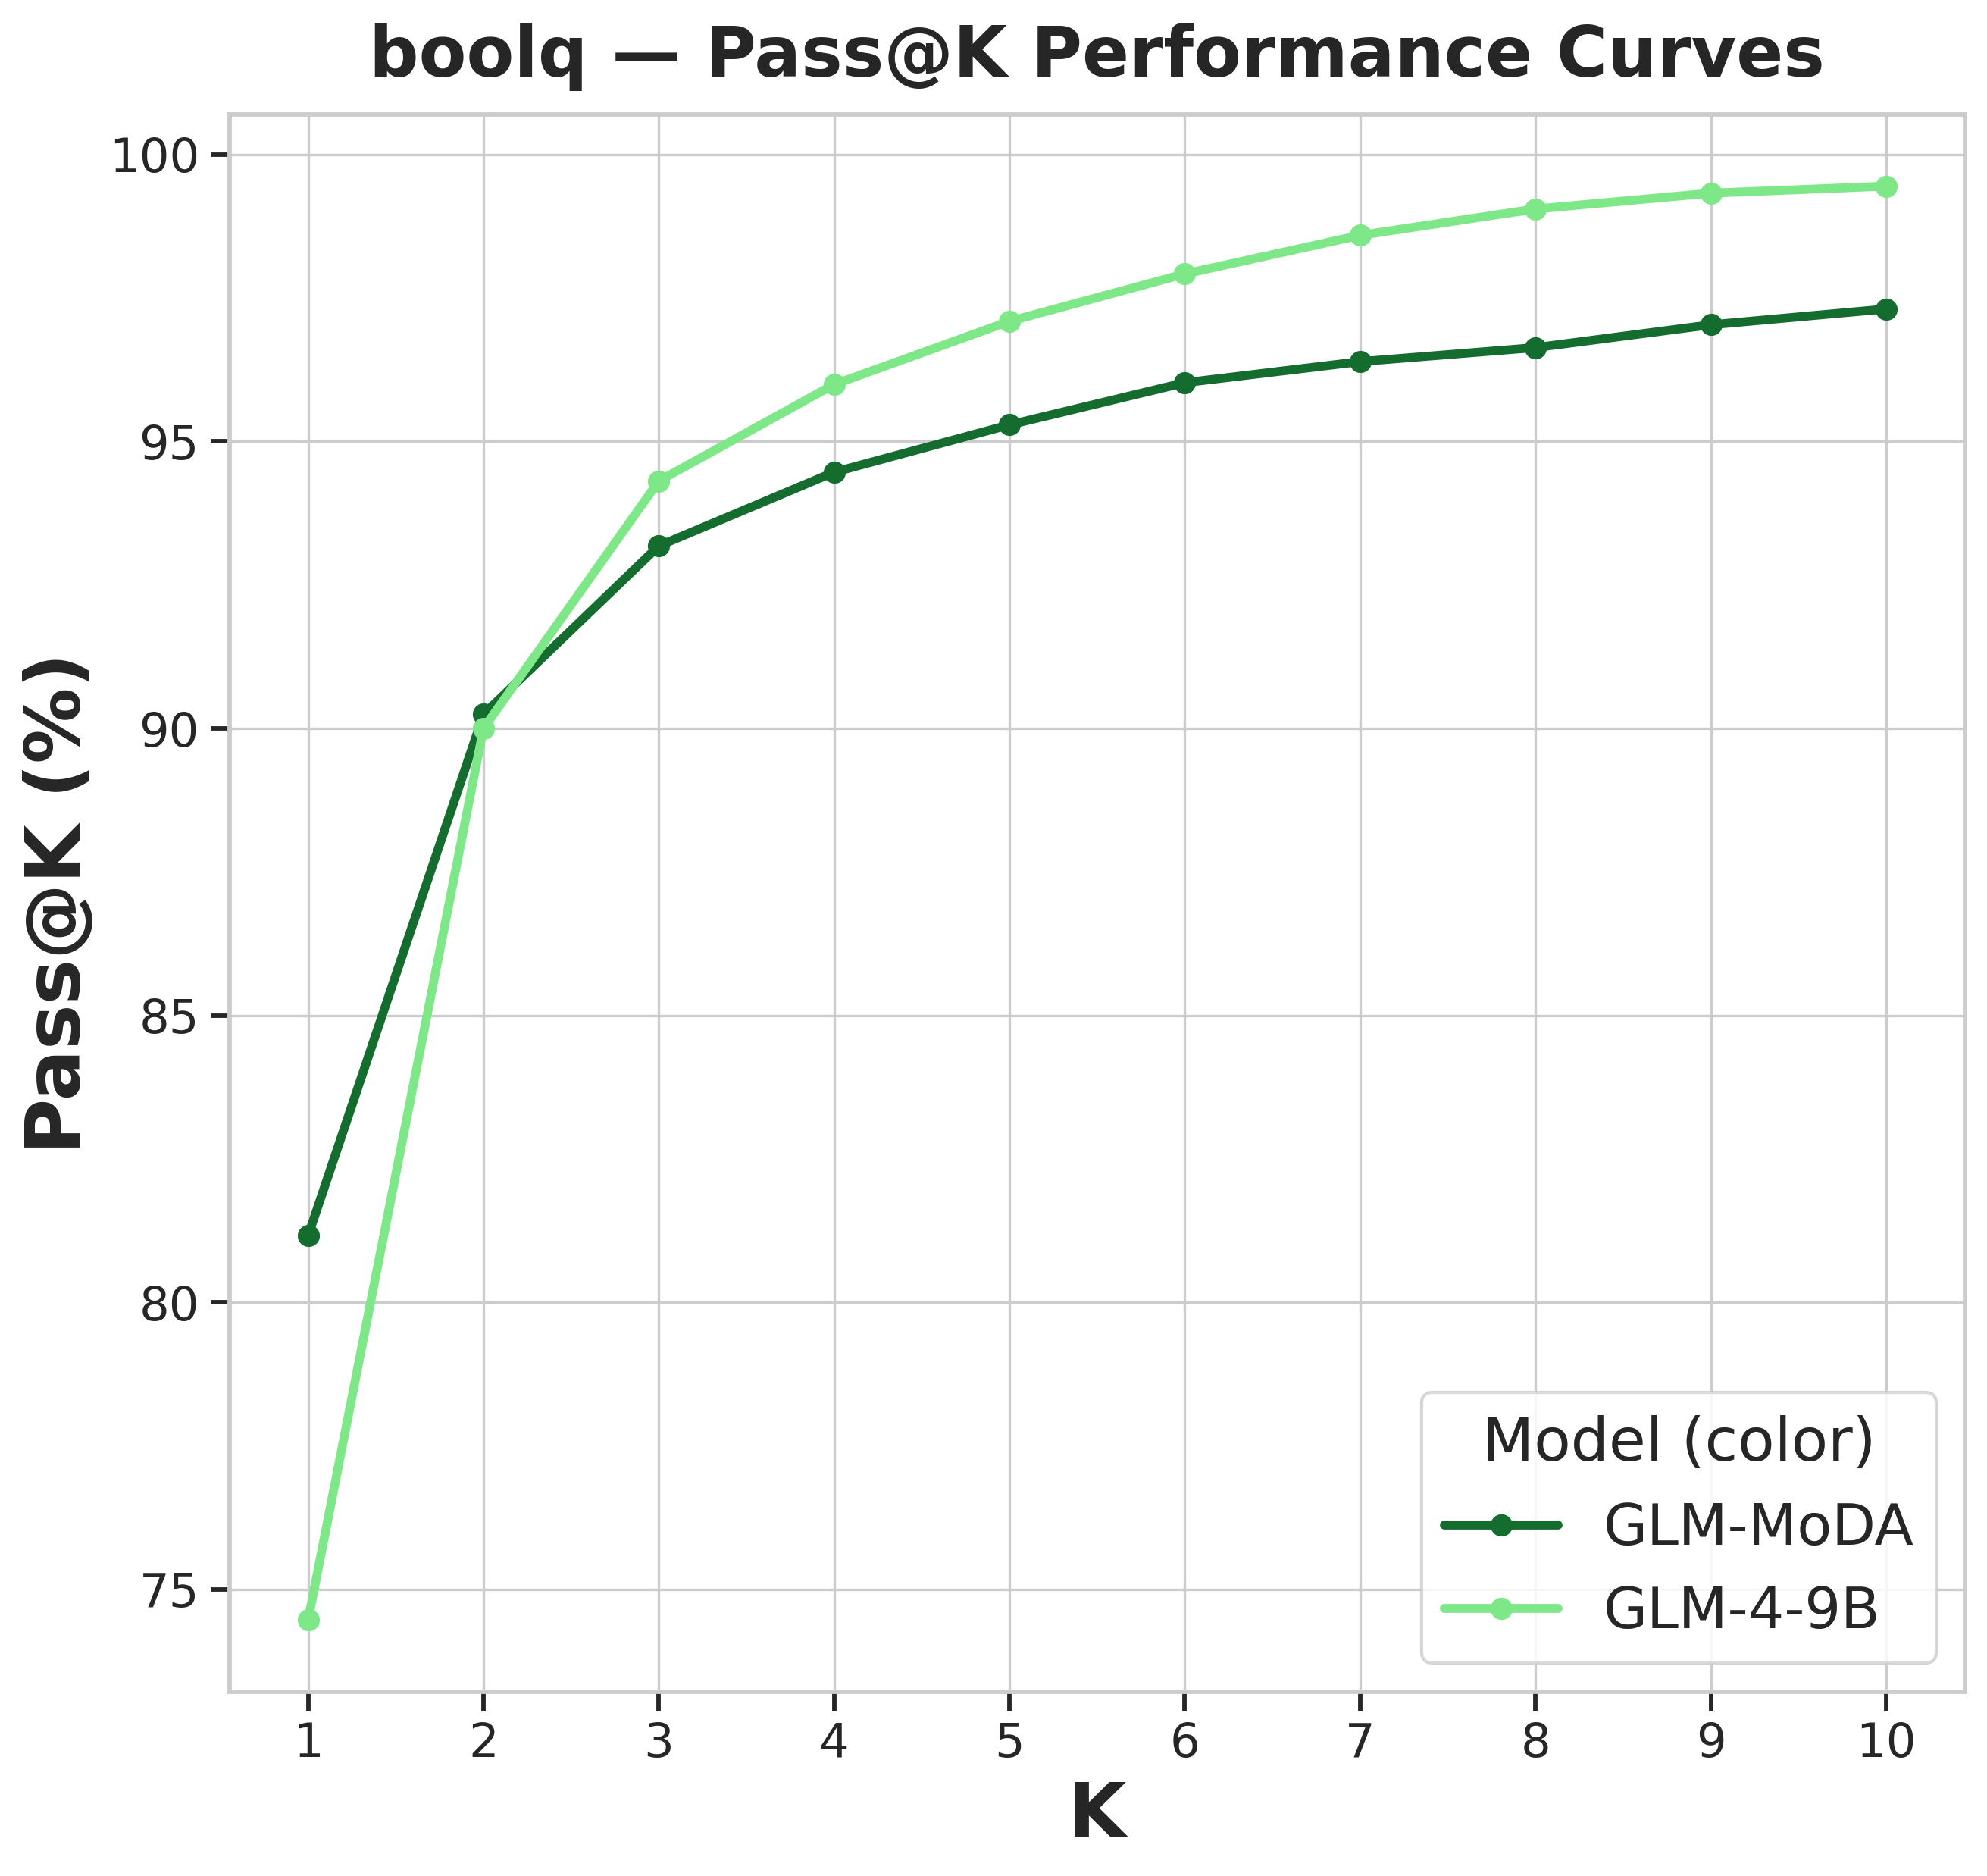
\includegraphics[width=\linewidth]{figures/main_pass_k/pass_at_k_figures/pass_at_k_boolq_thinking_false_base_model_glm-4-9b.png}
\end{minipage}\hfill
\centering
\begin{minipage}{0.24\textwidth}
  \centering
  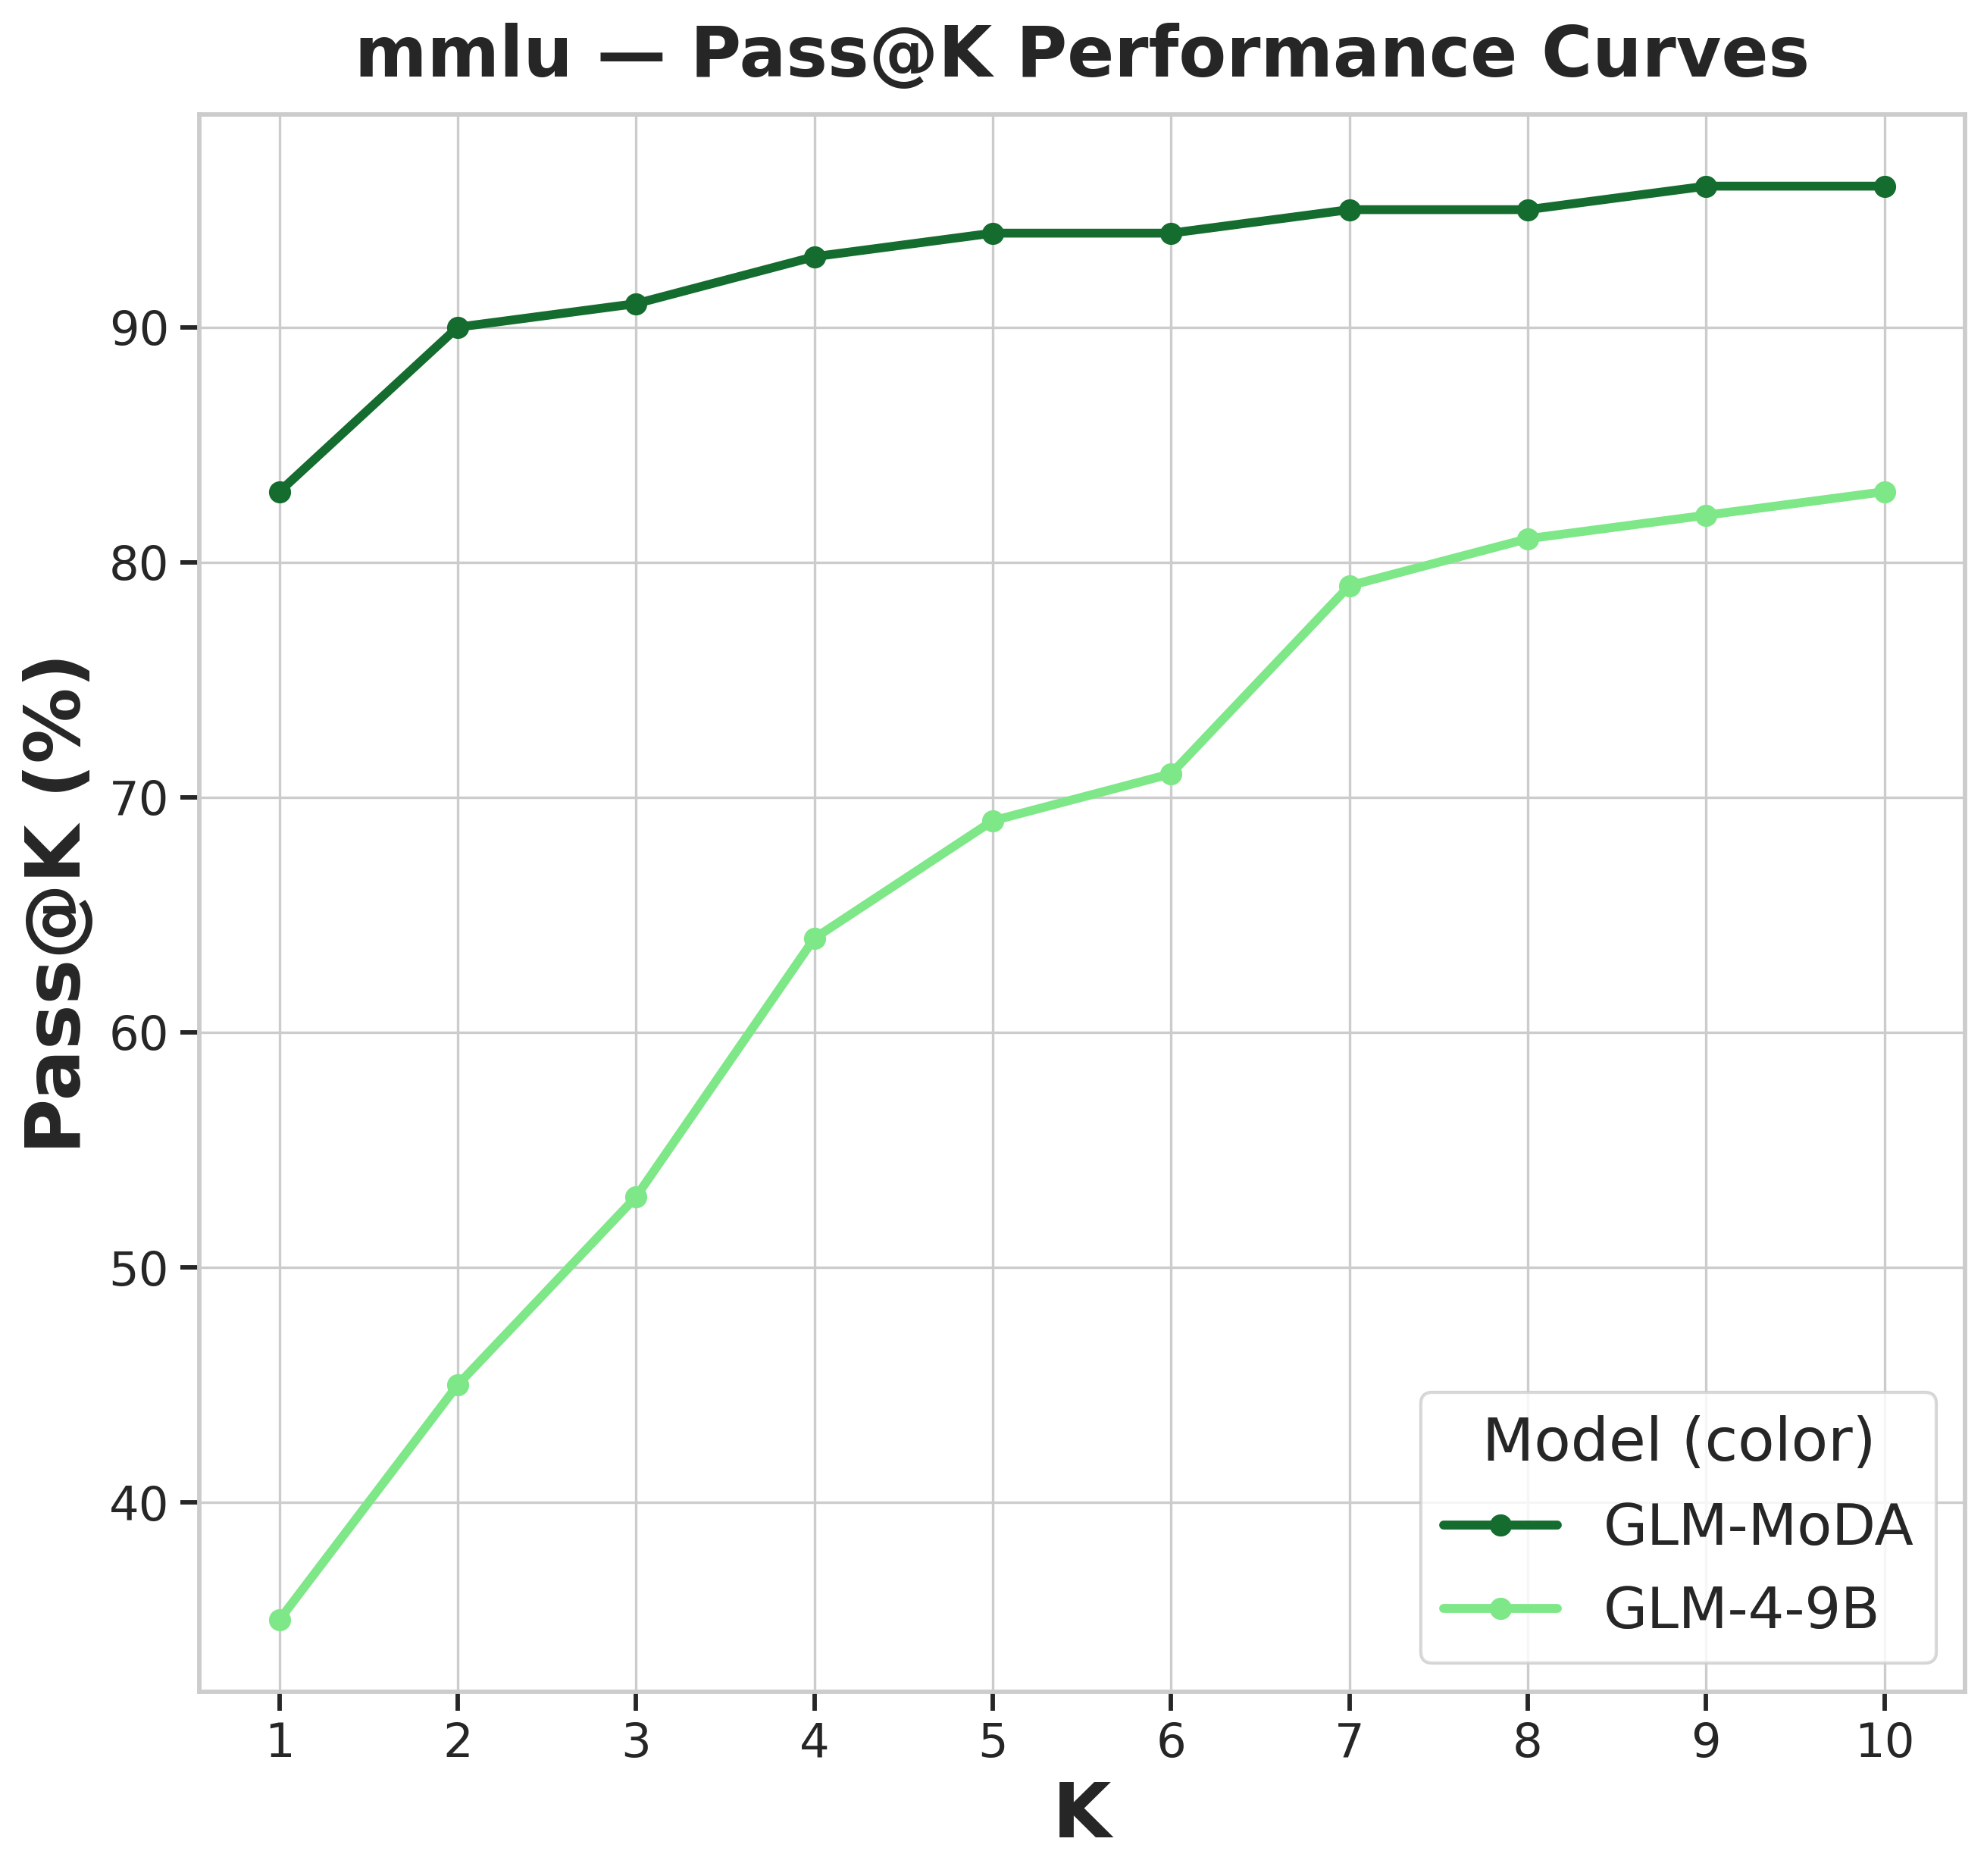
\includegraphics[width=\linewidth]{figures/main_pass_k/pass_at_k_figures/pass_at_k_mmlu_thinking_false_base_model_glm-4-9b.png}
\end{minipage}\hfill
\begin{minipage}{0.24\textwidth}
  \centering
  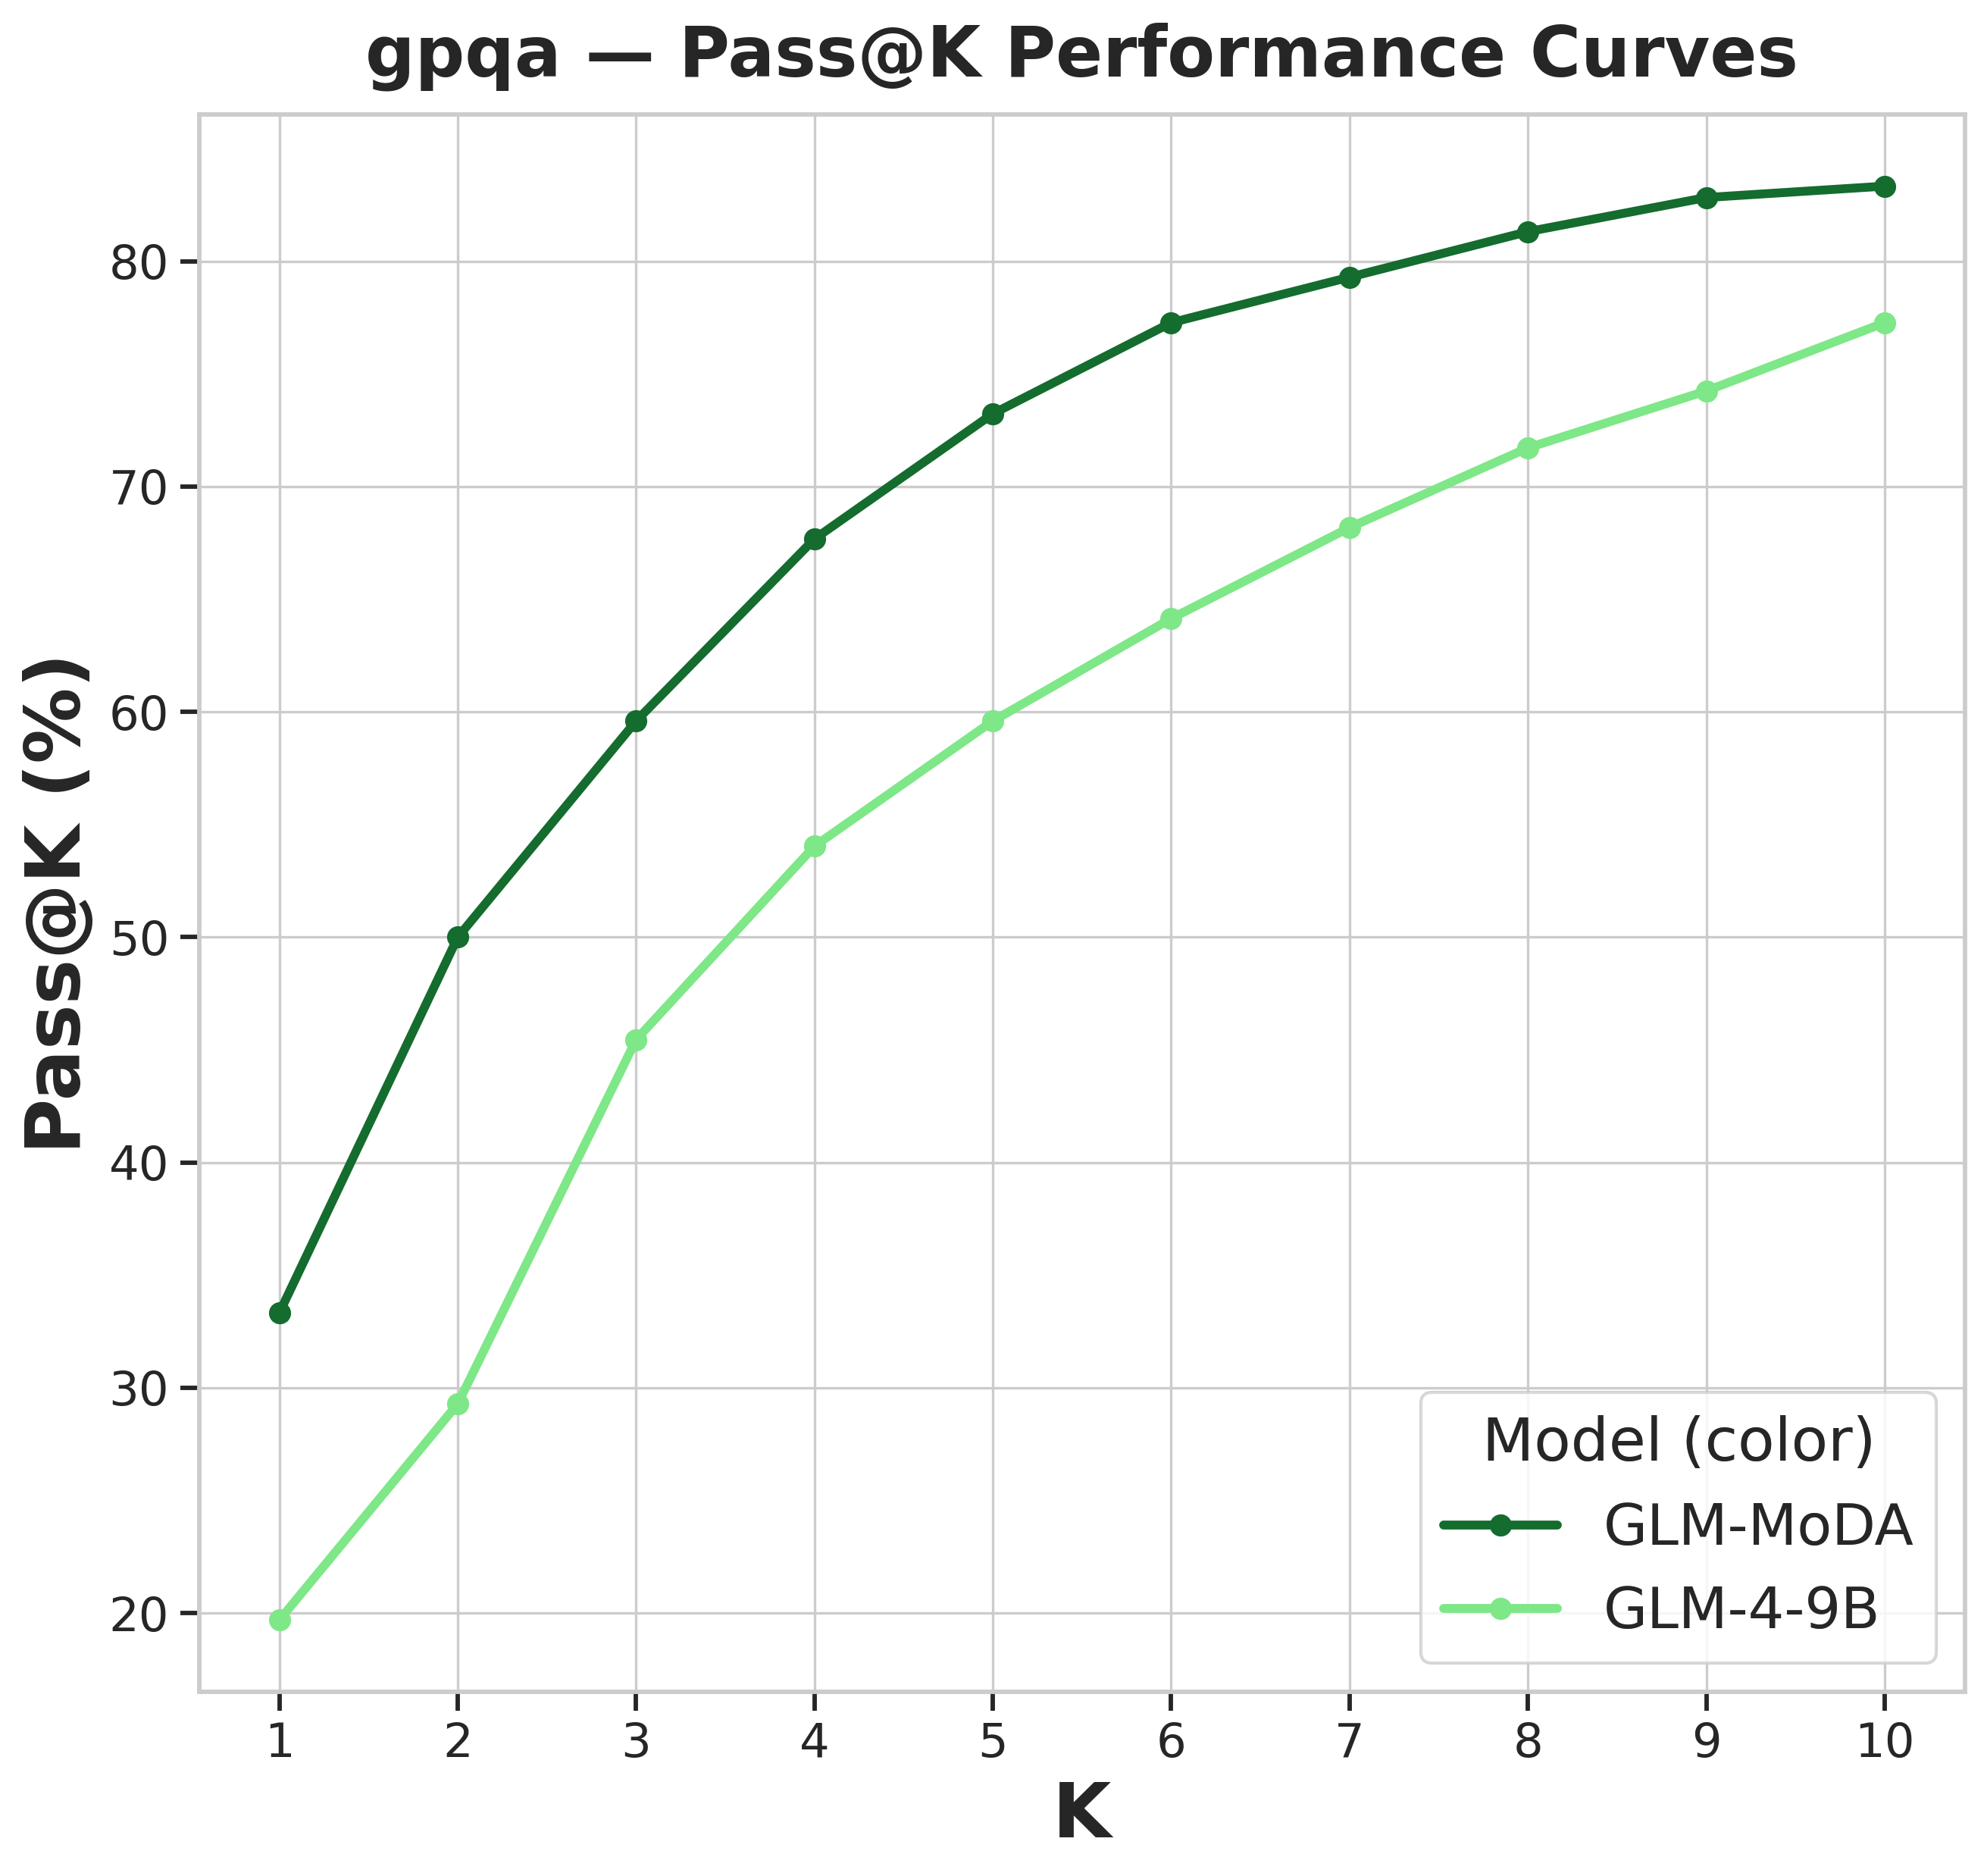
\includegraphics[width=\linewidth]{figures/main_pass_k/pass_at_k_figures/pass_at_k_gpqa_thinking_false_base_model_glm-4-9b.png}
\end{minipage}\hfill
\begin{minipage}{0.24\textwidth}
  \centering
  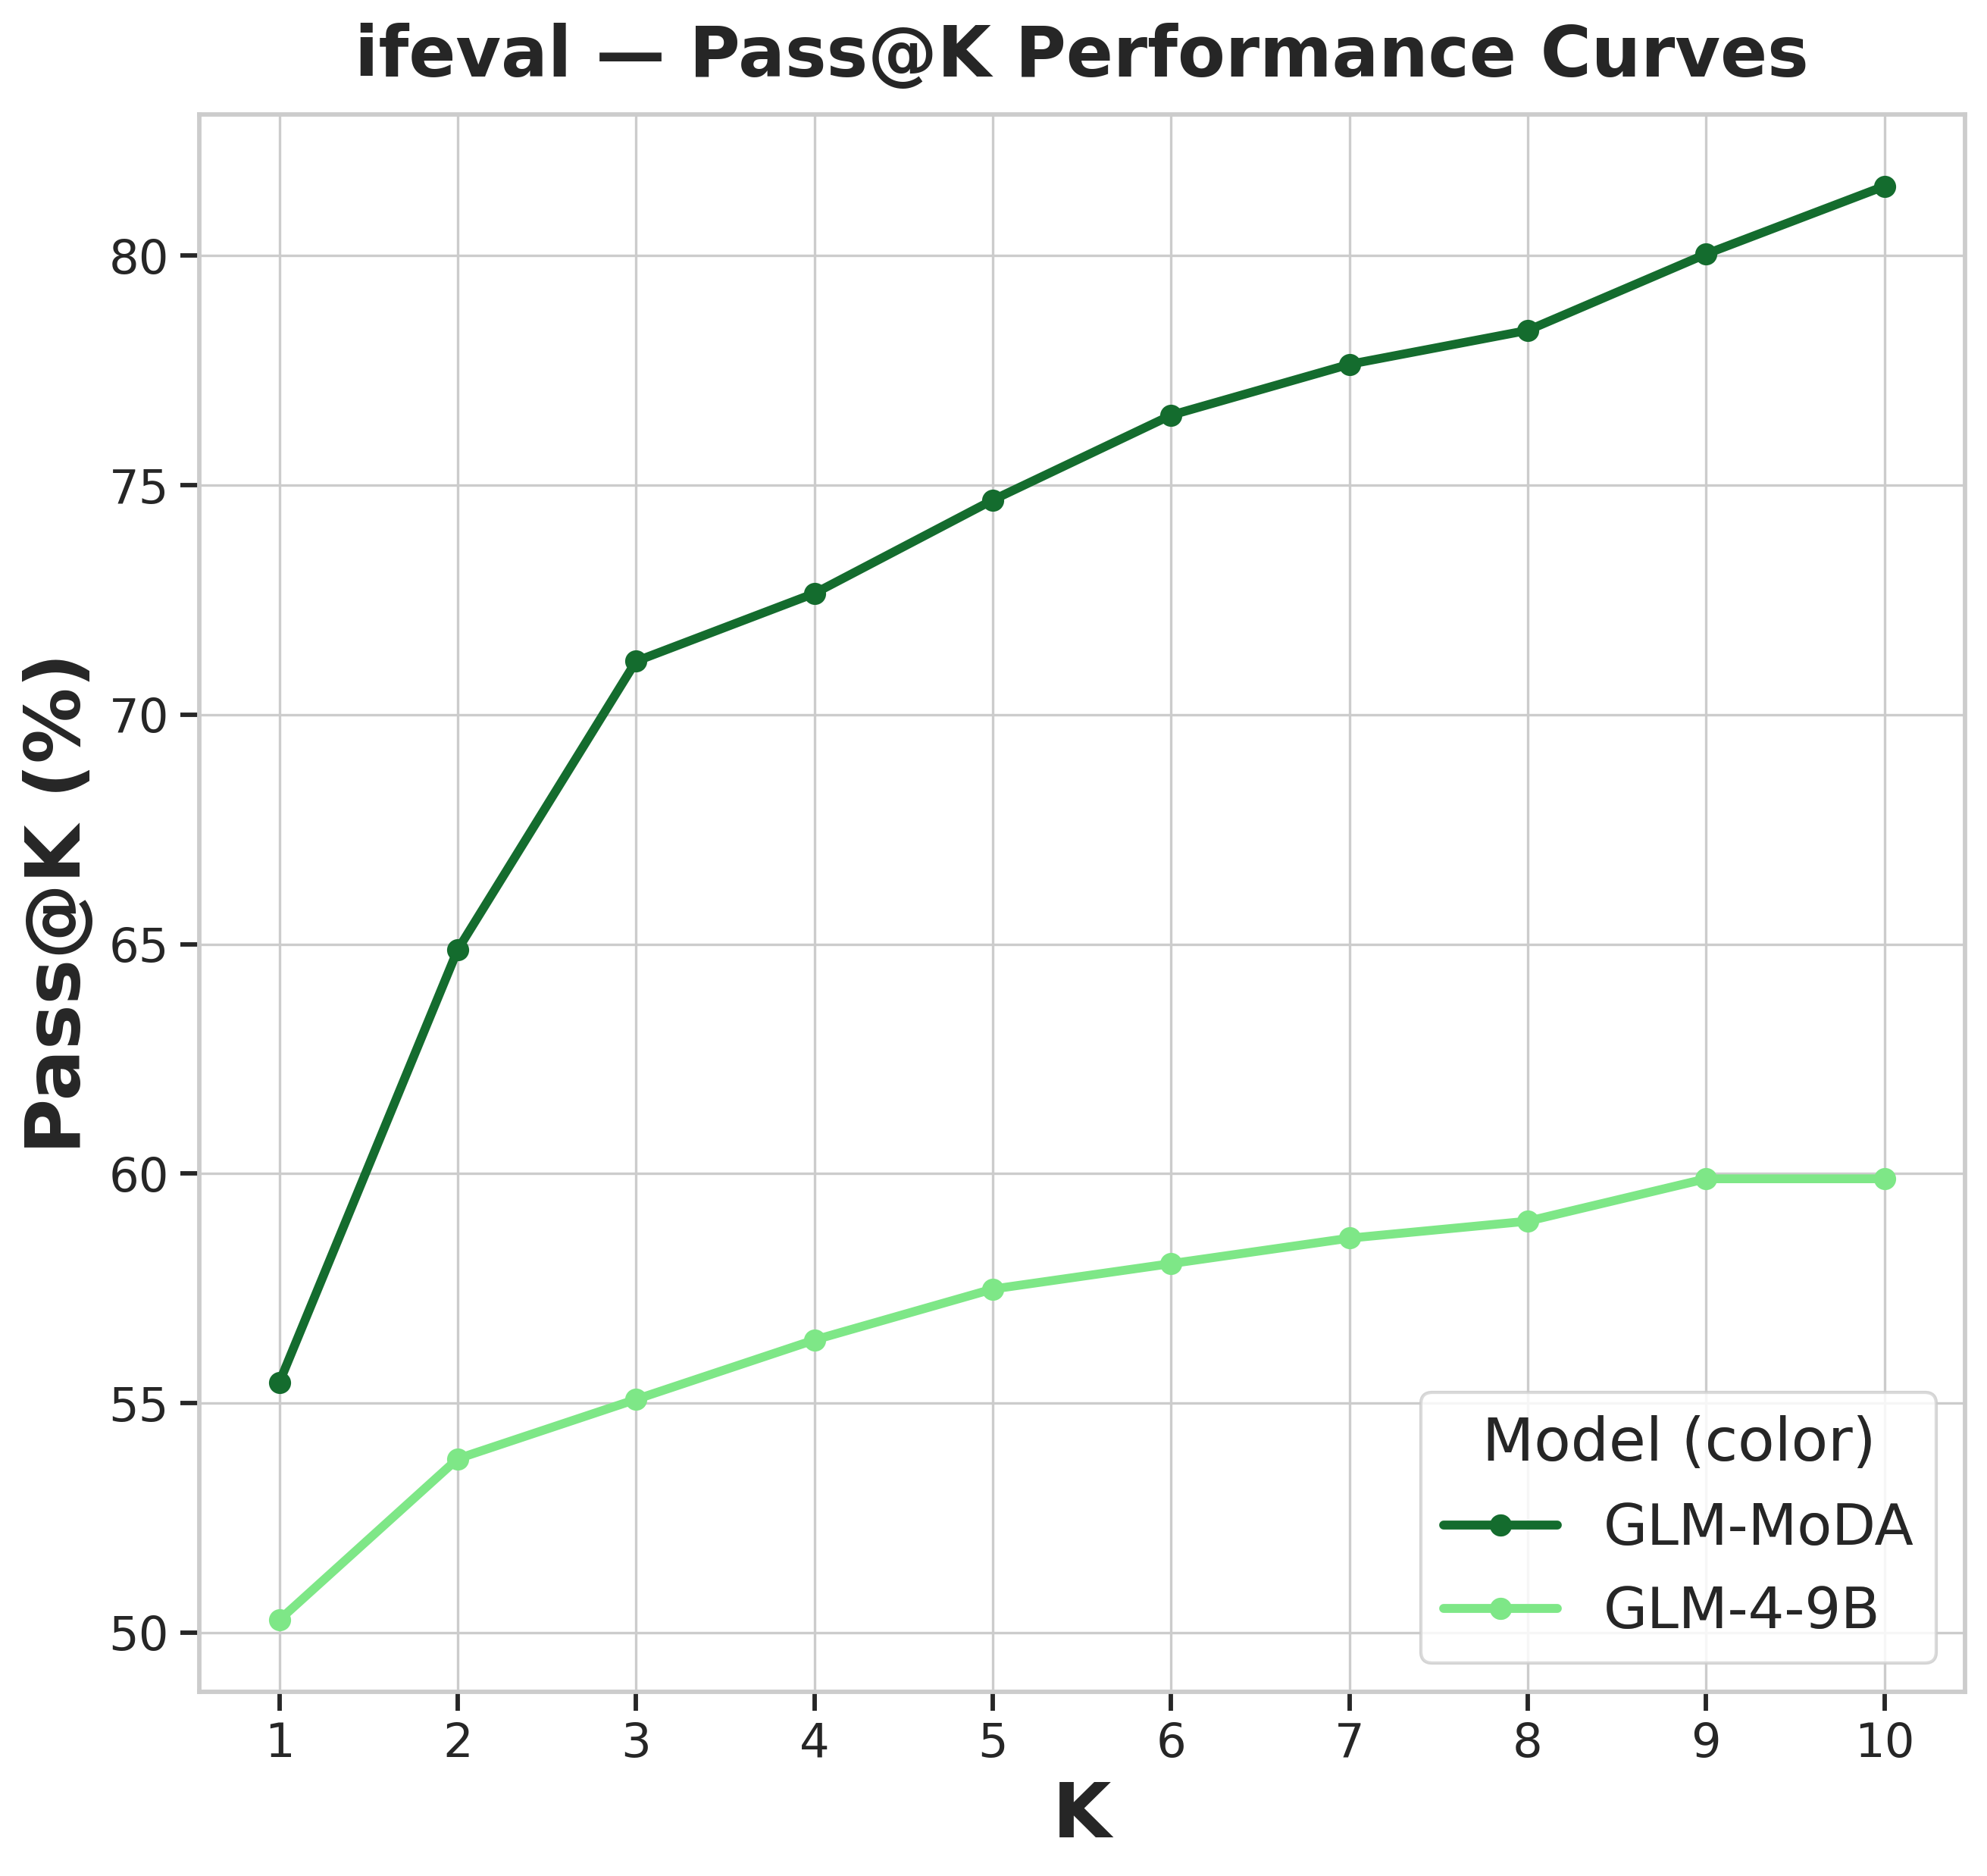
\includegraphics[width=\linewidth]{figures/main_pass_k/pass_at_k_figures/pass_at_k_ifeval_thinking_false_base_model_glm-4-9b.png}
\end{minipage}
\caption{\textbf{General capability retention: pass@k accuracy.} GLM-4-9B base and thinking disabled models.}
\label{fig:general capability pass@k glm}
\end{figure}

\subsection{Ablation Results}
\label{appx: ablation results}
We show the mean benchmark accuracy, under both standard and diverse decoding mode, on the general capability suite, and Infinite-Chat response diversity on the held out test set for the ablation study models.
\begin{table}[H]
\centering
\setlength{\tabcolsep}{3pt}
\resizebox{\textwidth}{!}{%
\begin{tabular}{lccccc}
\toprule
& \multicolumn{2}{c}{General capability (Avg., \%)} & \multicolumn{3}{c}{Infinite-Chat Diversity} \\
\cmidrule(lr){2-3} \cmidrule(lr){4-6}
Ablation & Standard mode & Diverse mode & Disc. & SBERT & E-Vendi \\
\midrule
Role-conditioned prompting & 62.9  & 56.6  & 0.403  & 0.145  & 1.90  \\
Quality only & 63.2  & 61.8  & 0.401  & 0.131  & 1.82  \\
Diversity only & 61.1  & 10.7  & \textbf{0.656}  & \textbf{0.993}  & \textbf{9.77}  \\
Additive $w{=}1$ & 67.4  & 68.0  & 0.422  & 0.204  & 2.33  \\
Additive $w{=}10$ & 64.5  & 5.7  & 0.632  & 0.976  & 9.64  \\
Additive $w{=}100$ & 61.6  & 5.4  & 0.621  & 0.970  & 8.75  \\
Token-based roles & 69.7  & 67.9 & 0.419 & 0.197 & 2.04 \\
Crafted personas & 70.1  & 66.1  & 0.421  & 0.194  & 2.24  \\
Single role & 69.0  & 69.9  & 0.428  & 0.239  & 2.57  \\
\midrule
Qwen3-8B & 62.9 & - & 0.400 & 0.132 & 1.83 \\
\midrule
\textbf{\method{}} & \textbf{73.2}  & \textbf{71.6}  & 0.444  & 0.257  & 2.69  \\
\bottomrule
\end{tabular}
}
\vspace{4pt}
\caption{\textbf{Ablation results} for general capability (Pass@1) under standard and diverse decoding (accuracy \%) and Infinite-Chat diversity ($n{=}3$ random seeds). Bold marks the best value per column.}
\label{tab:ablation}
\vspace{-0.6cm}
\end{table}

\begin{figure}
\begin{minipage}{0.32\textwidth}
  \centering
  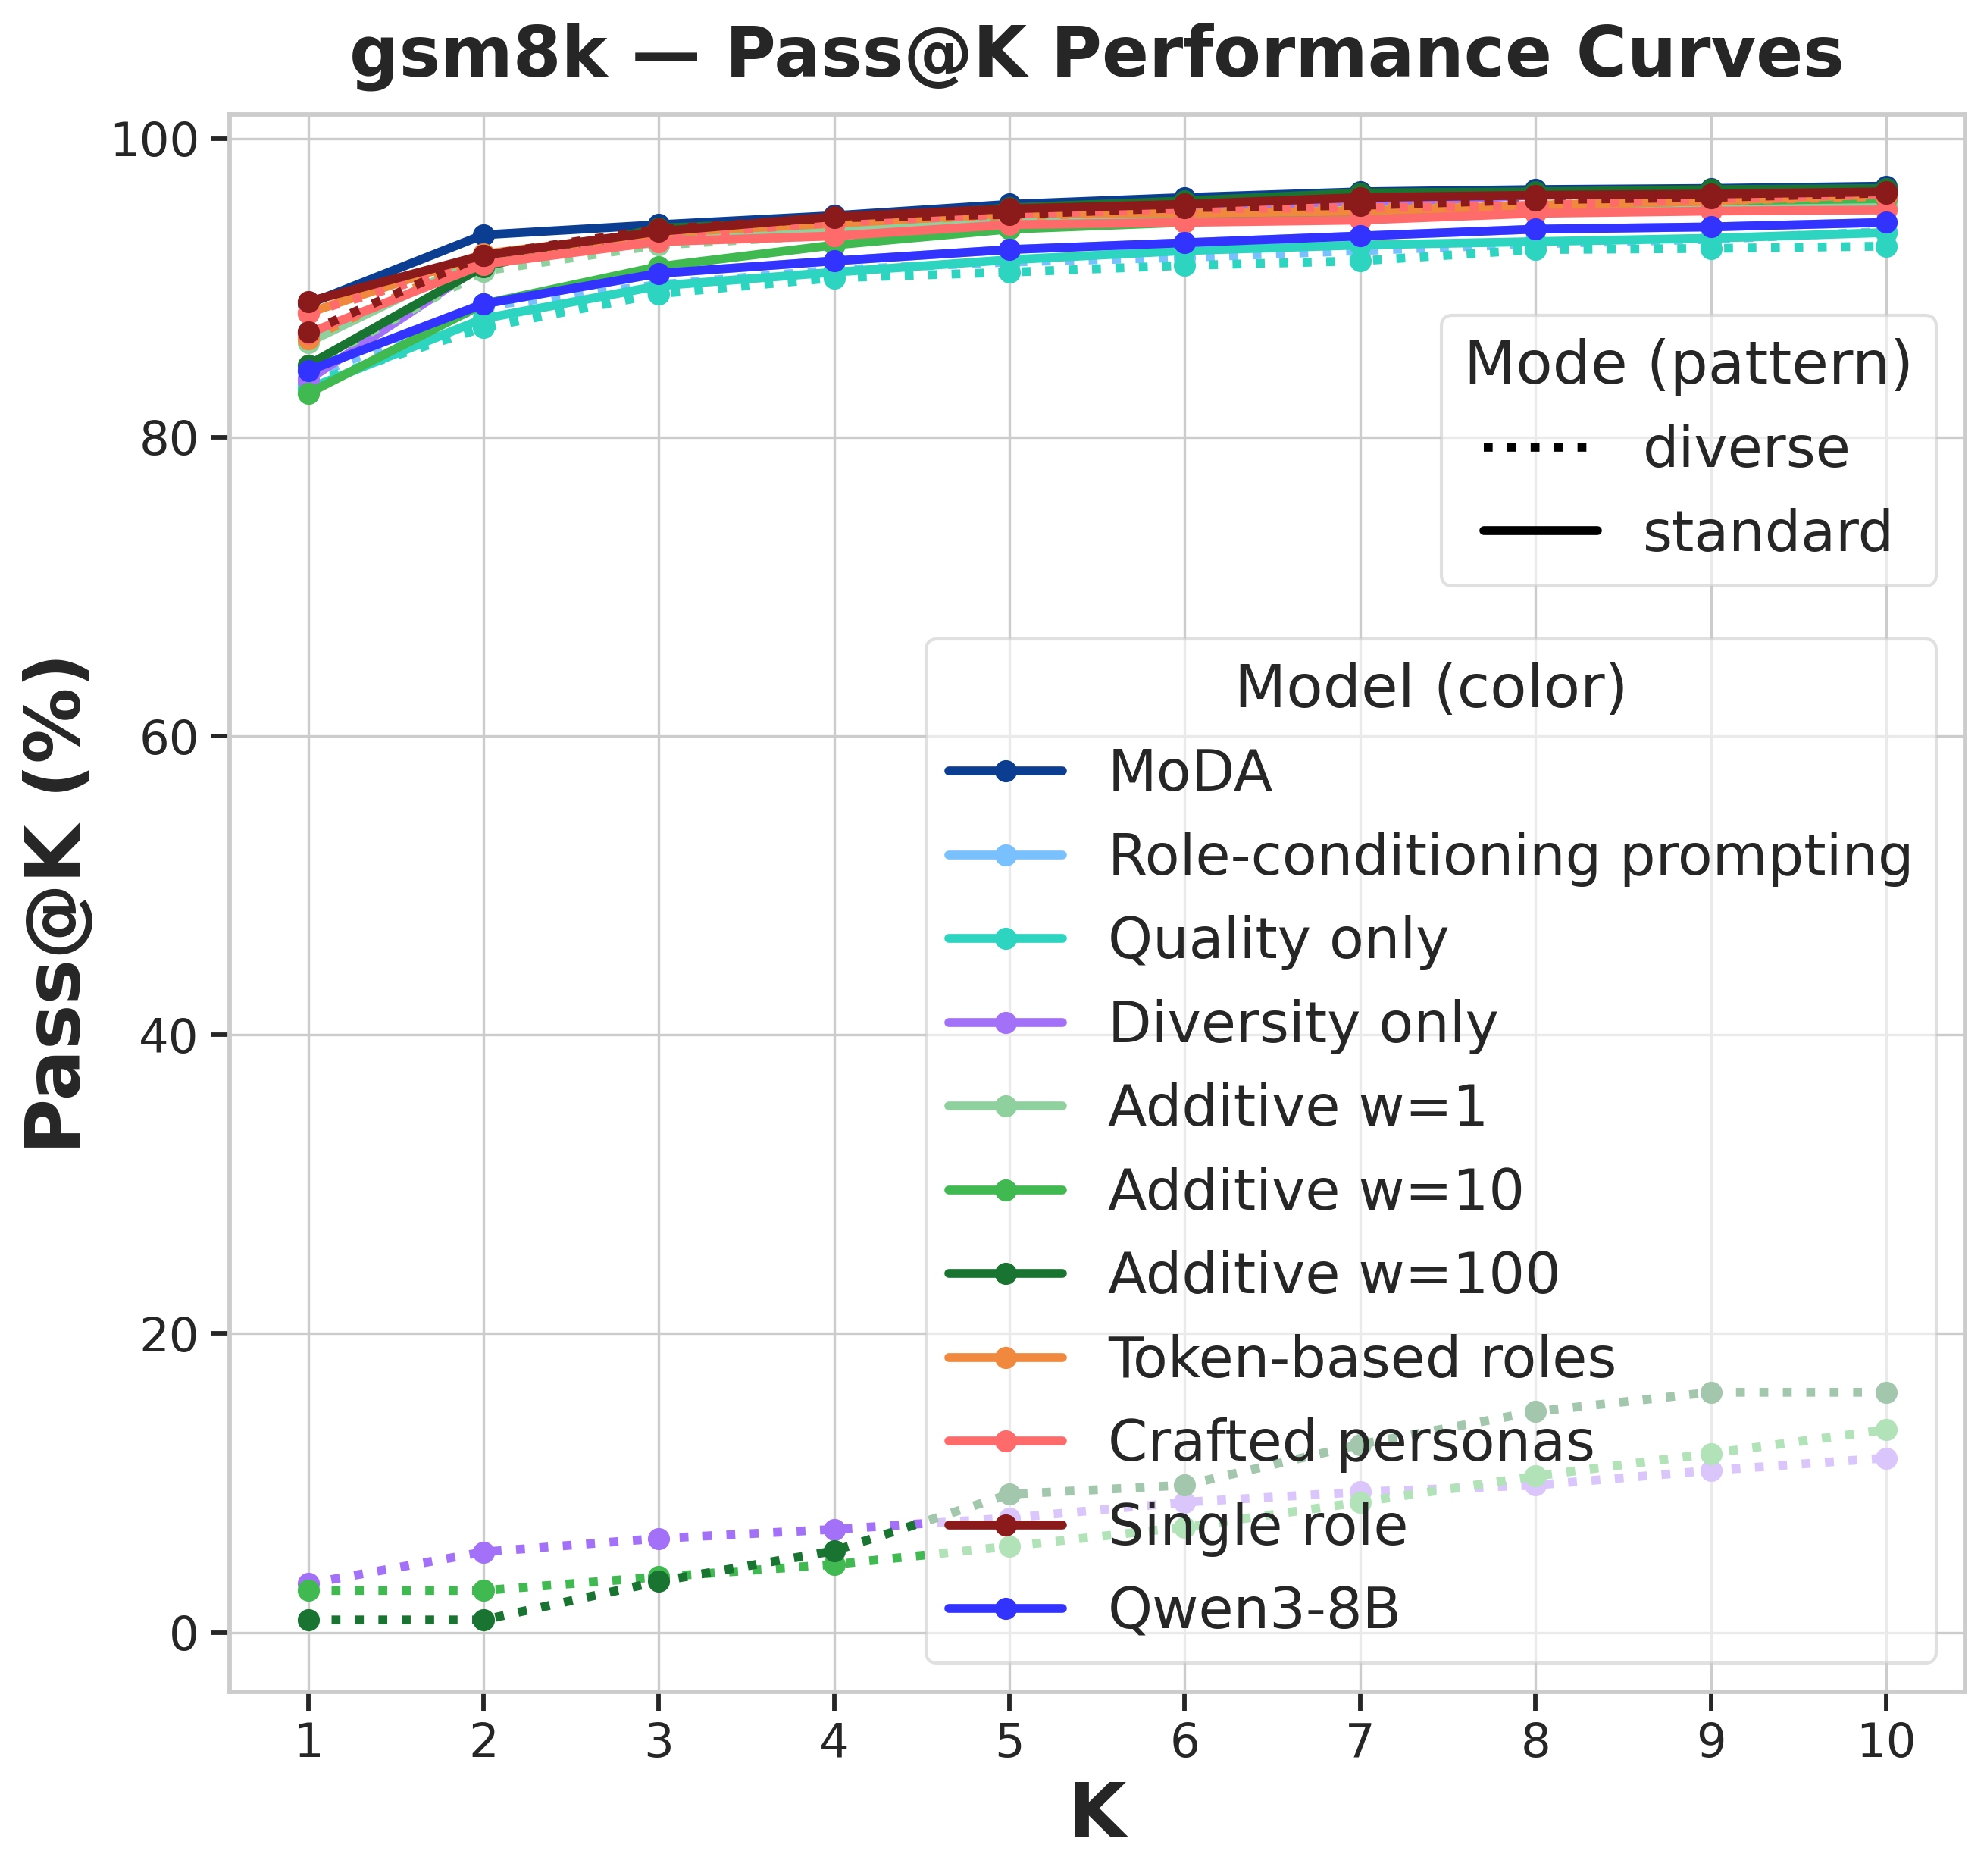
\includegraphics[width=\linewidth]{figures/ablation_pass_k/pass_at_k_gsm8k_ablations.png}
  \small Pass@k, GSM8K
  \label{fig: ablation pass@k GSM8K}
\end{minipage}\hfill
\centering
\begin{minipage}{0.32\textwidth}
  \centering
  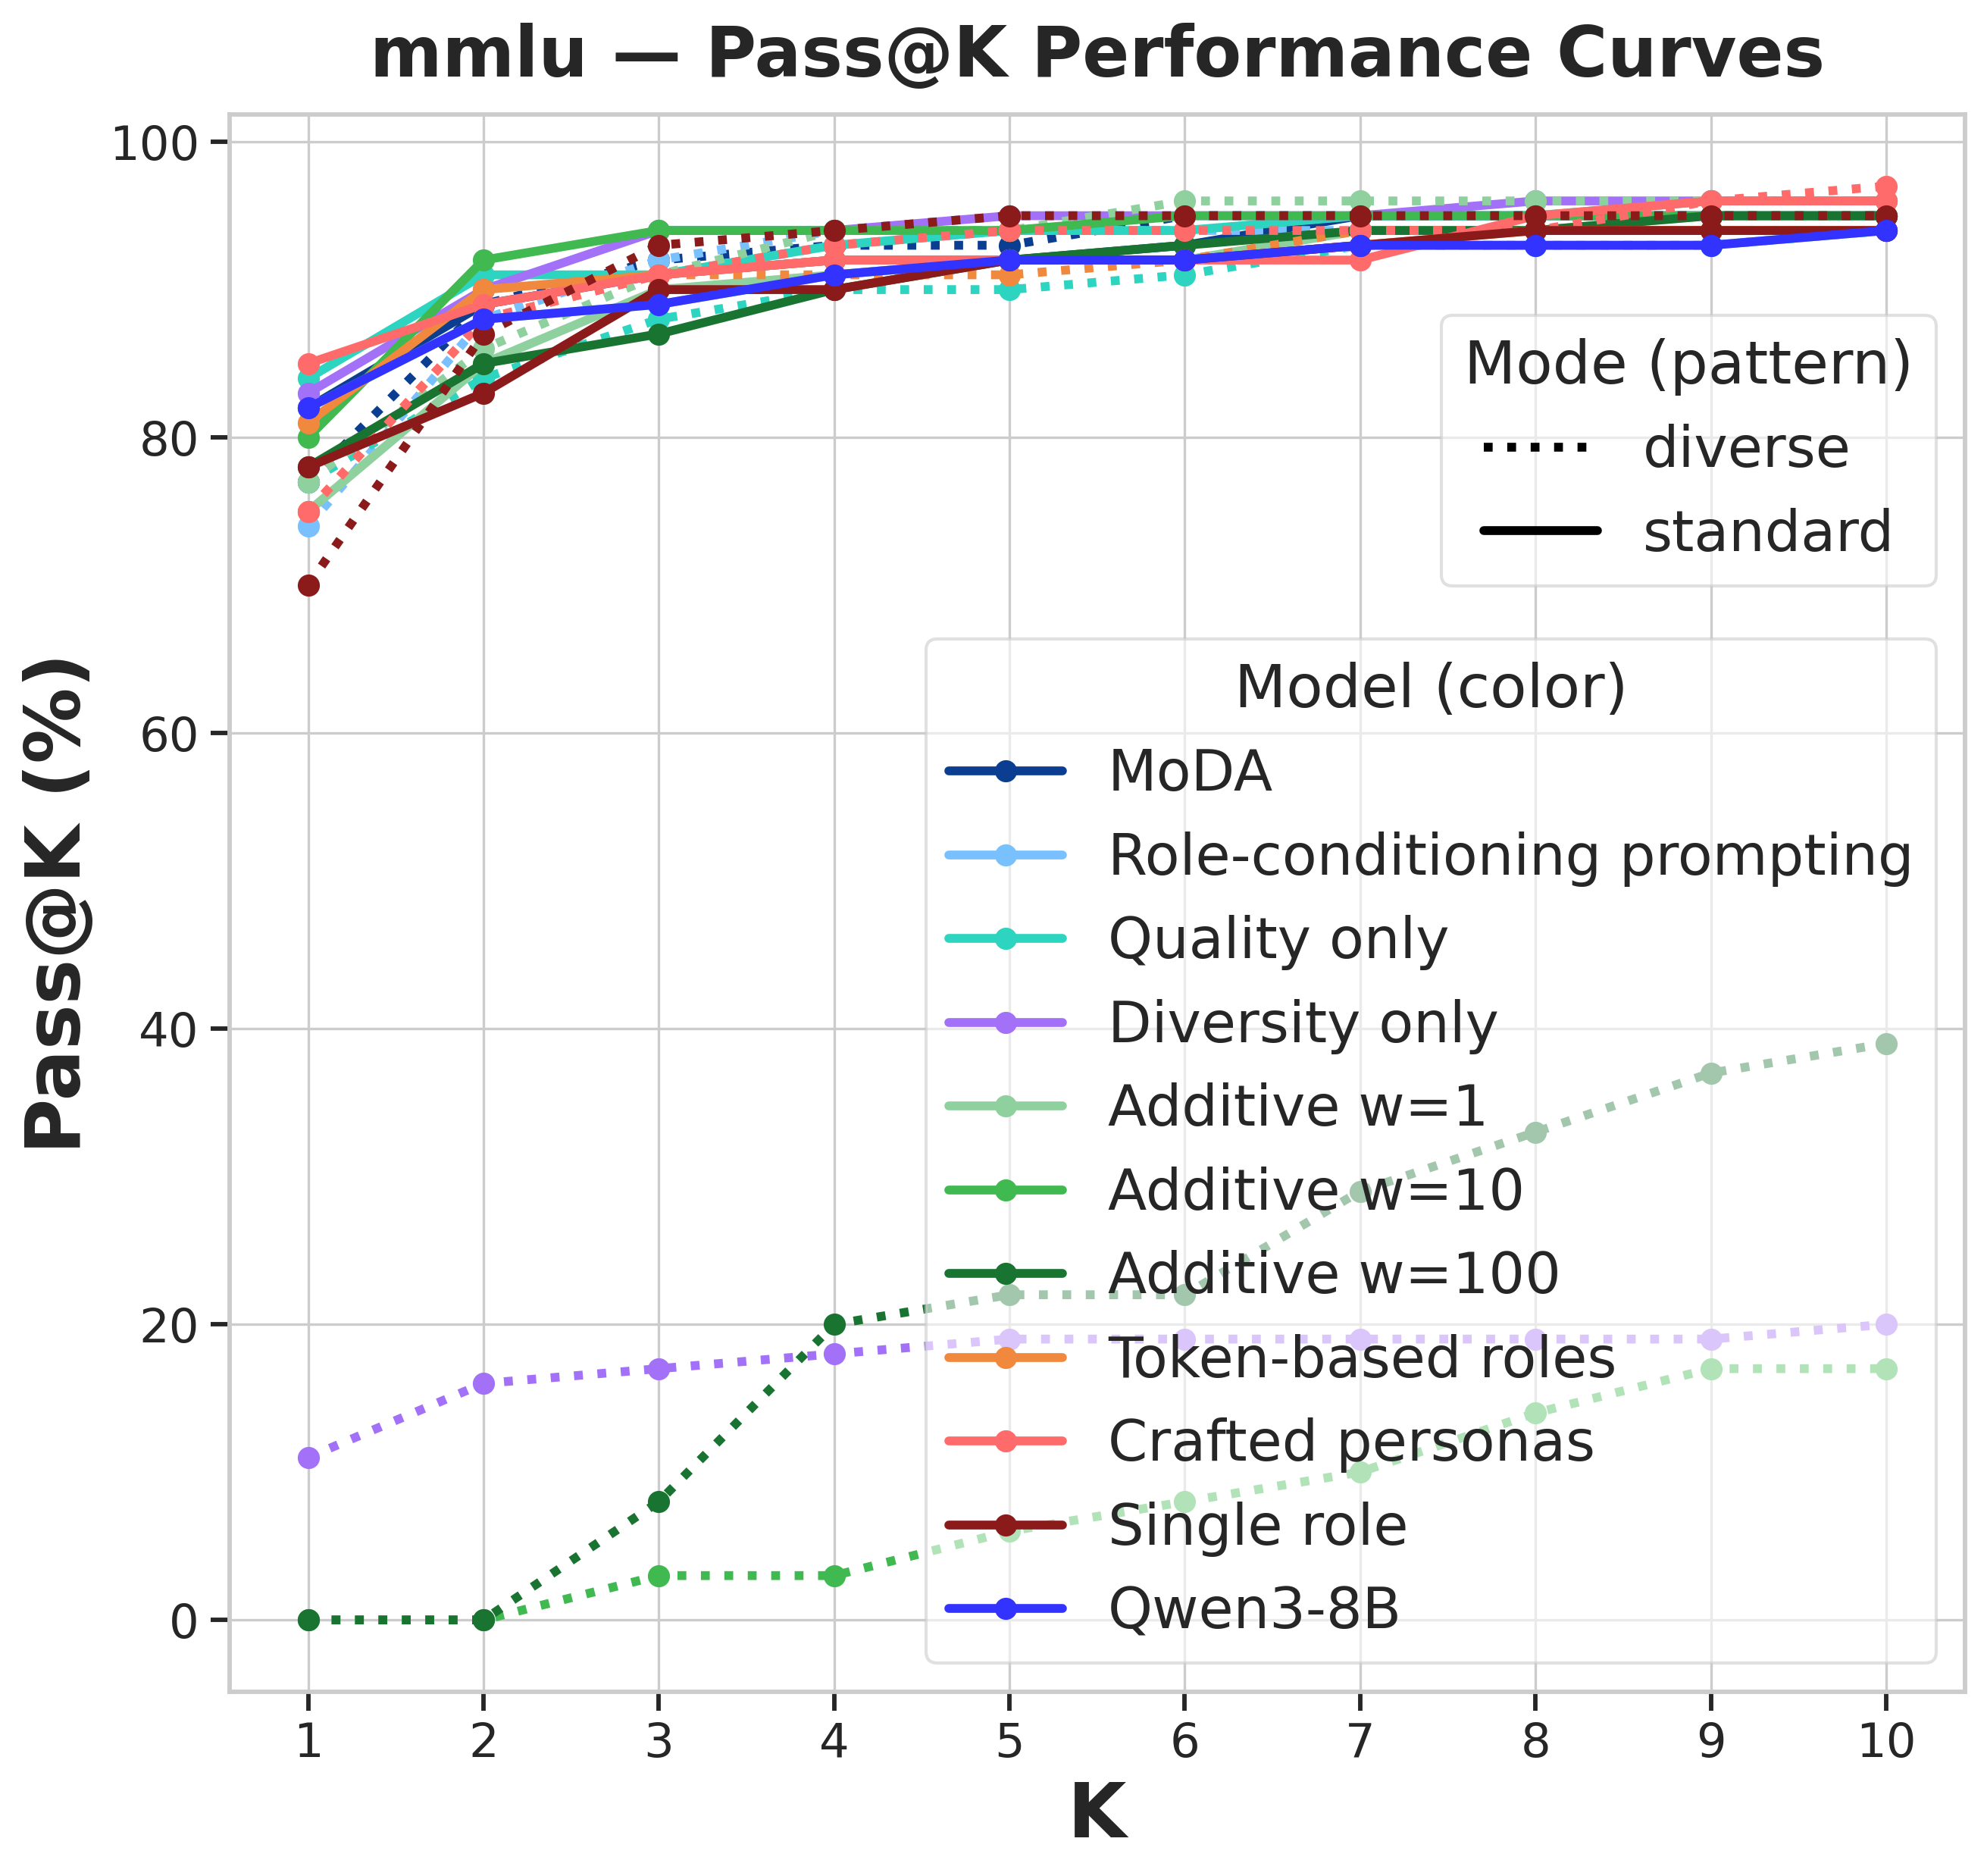
\includegraphics[width=\linewidth]{figures/ablation_pass_k/pass_at_k_mmlu_ablations.png}
  \small Pass@k, MMLU
  \label{fig: ablation pass@k MMLU}
\end{minipage}\hfill
\centering
\begin{minipage}{0.32\textwidth}
  \centering
  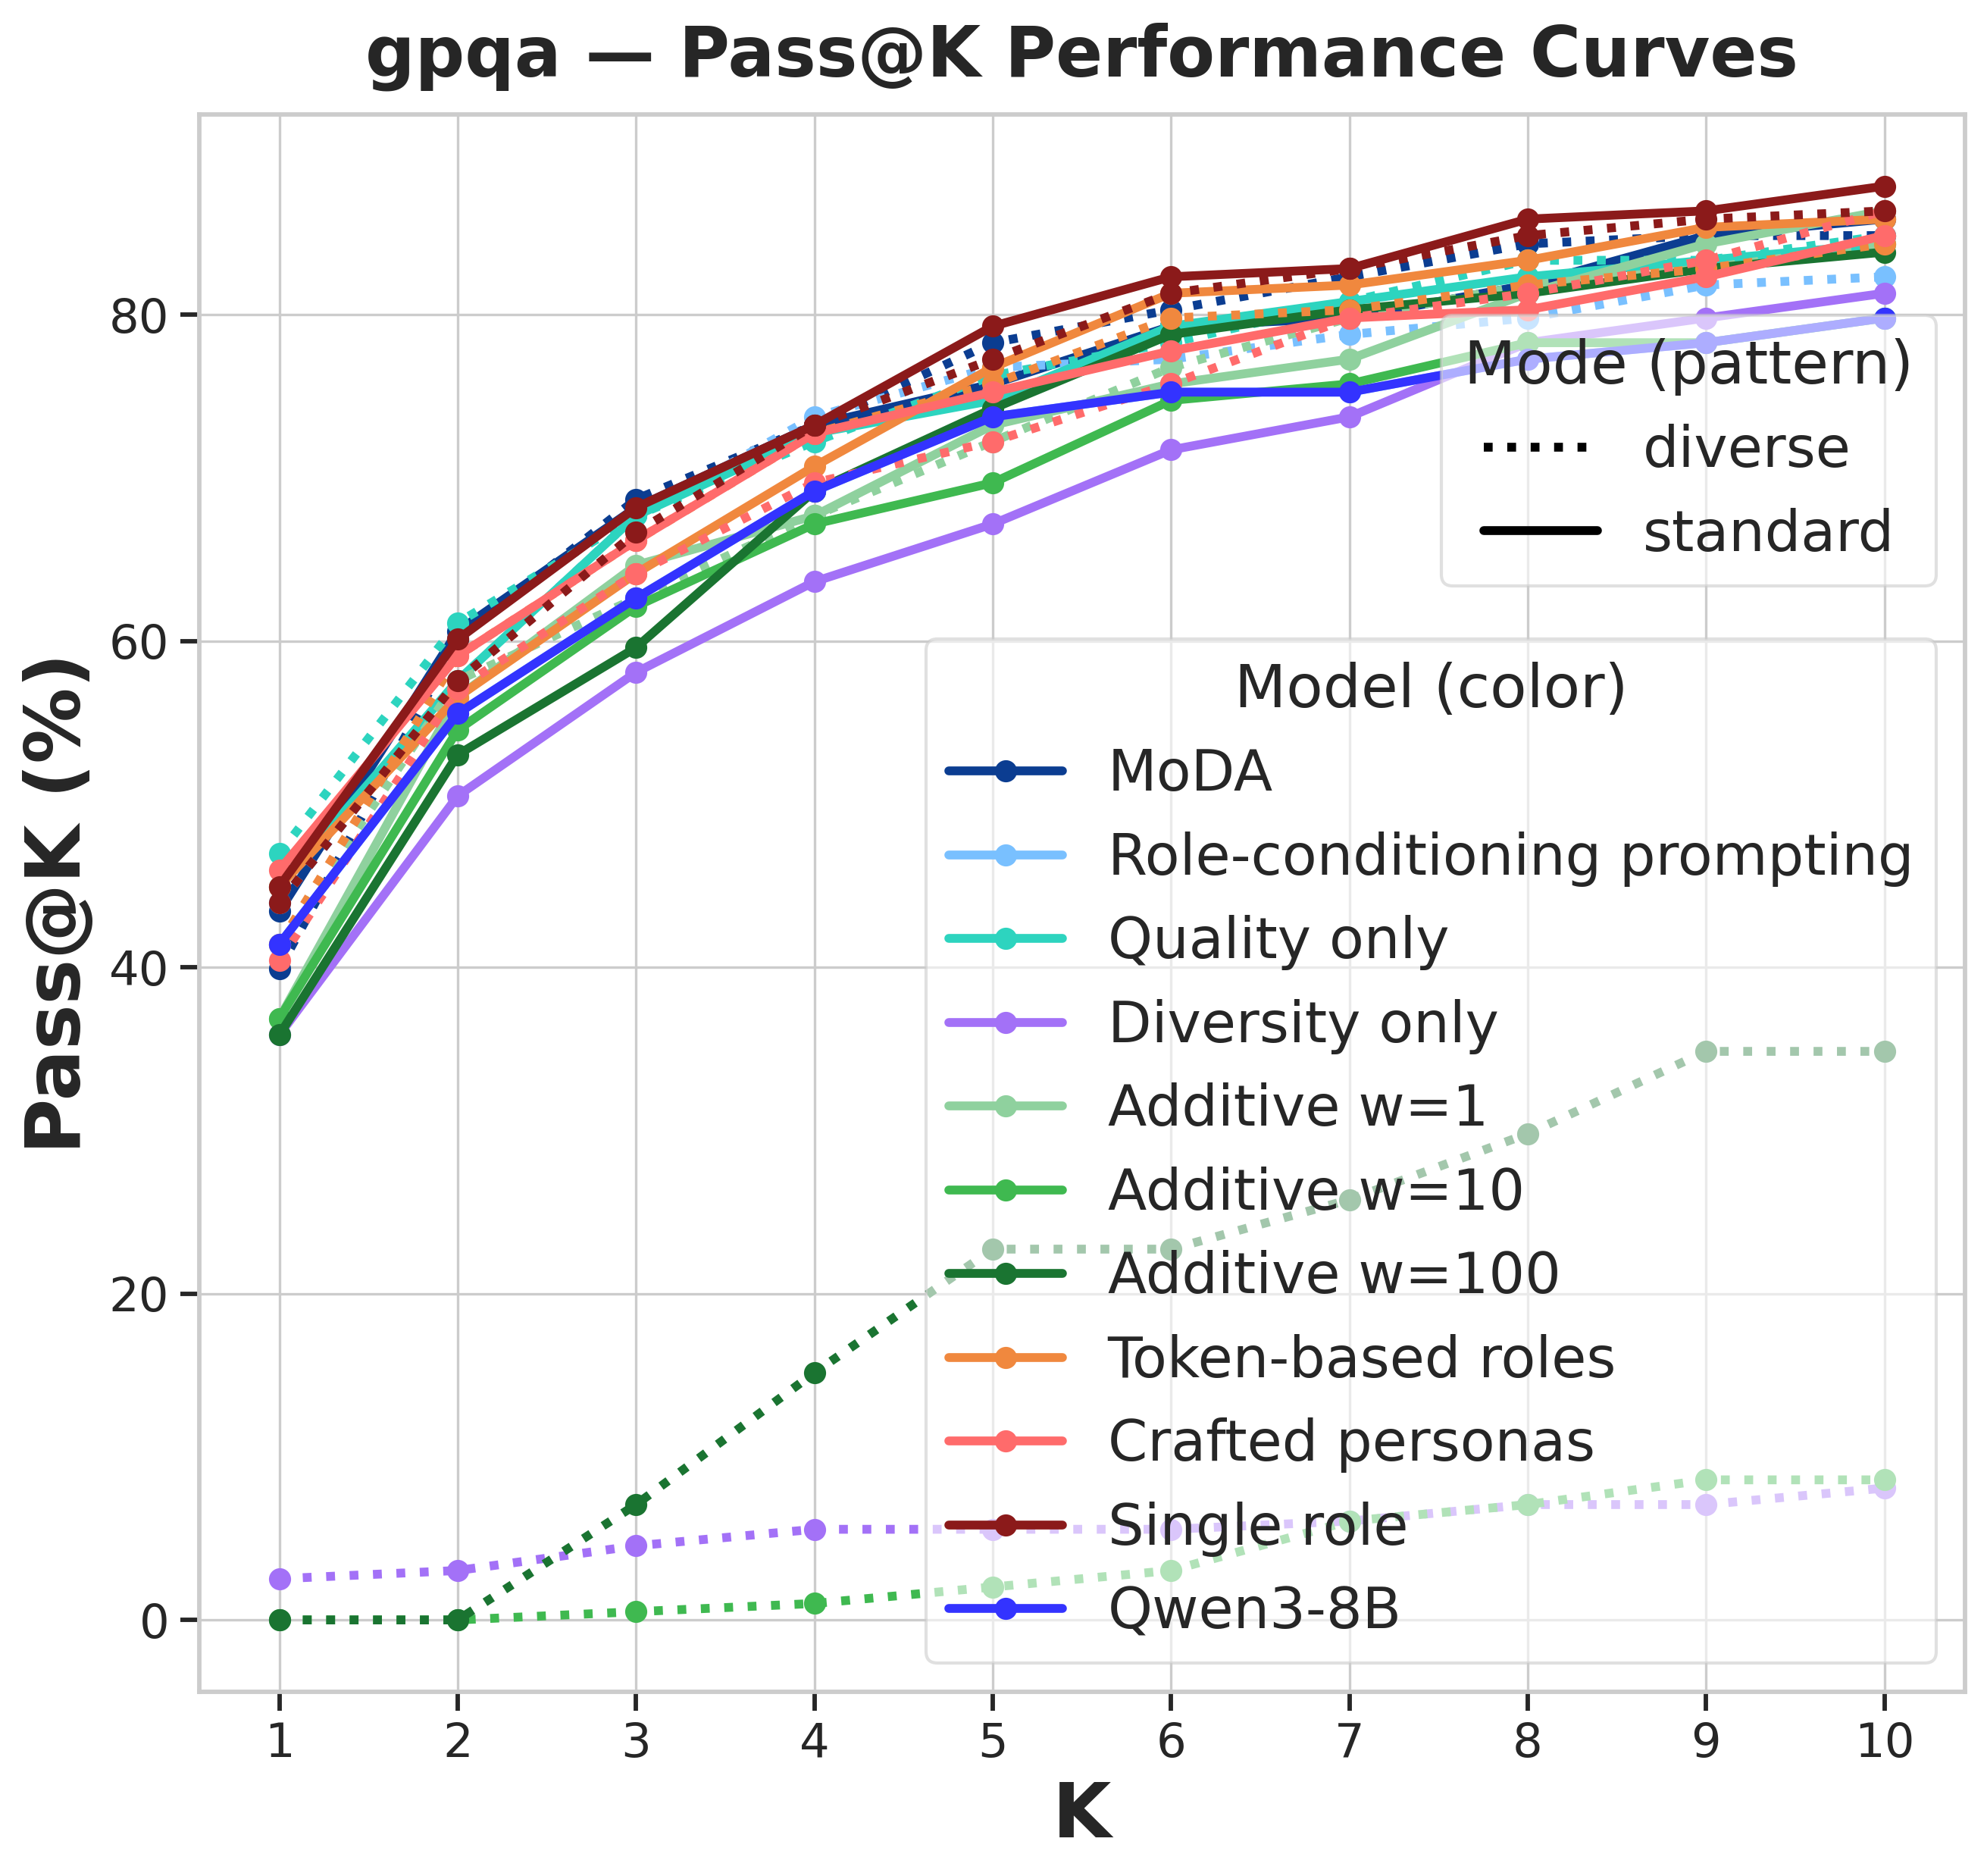
\includegraphics[width=\linewidth]{figures/ablation_pass_k/pass_at_k_gpqa_ablations.png}
  \small Pass@k, GPQA
  \label{fig: ablation pass@k GPQA}
\end{minipage}\hfill
\centering
\begin{minipage}{0.32\textwidth}
  \centering
  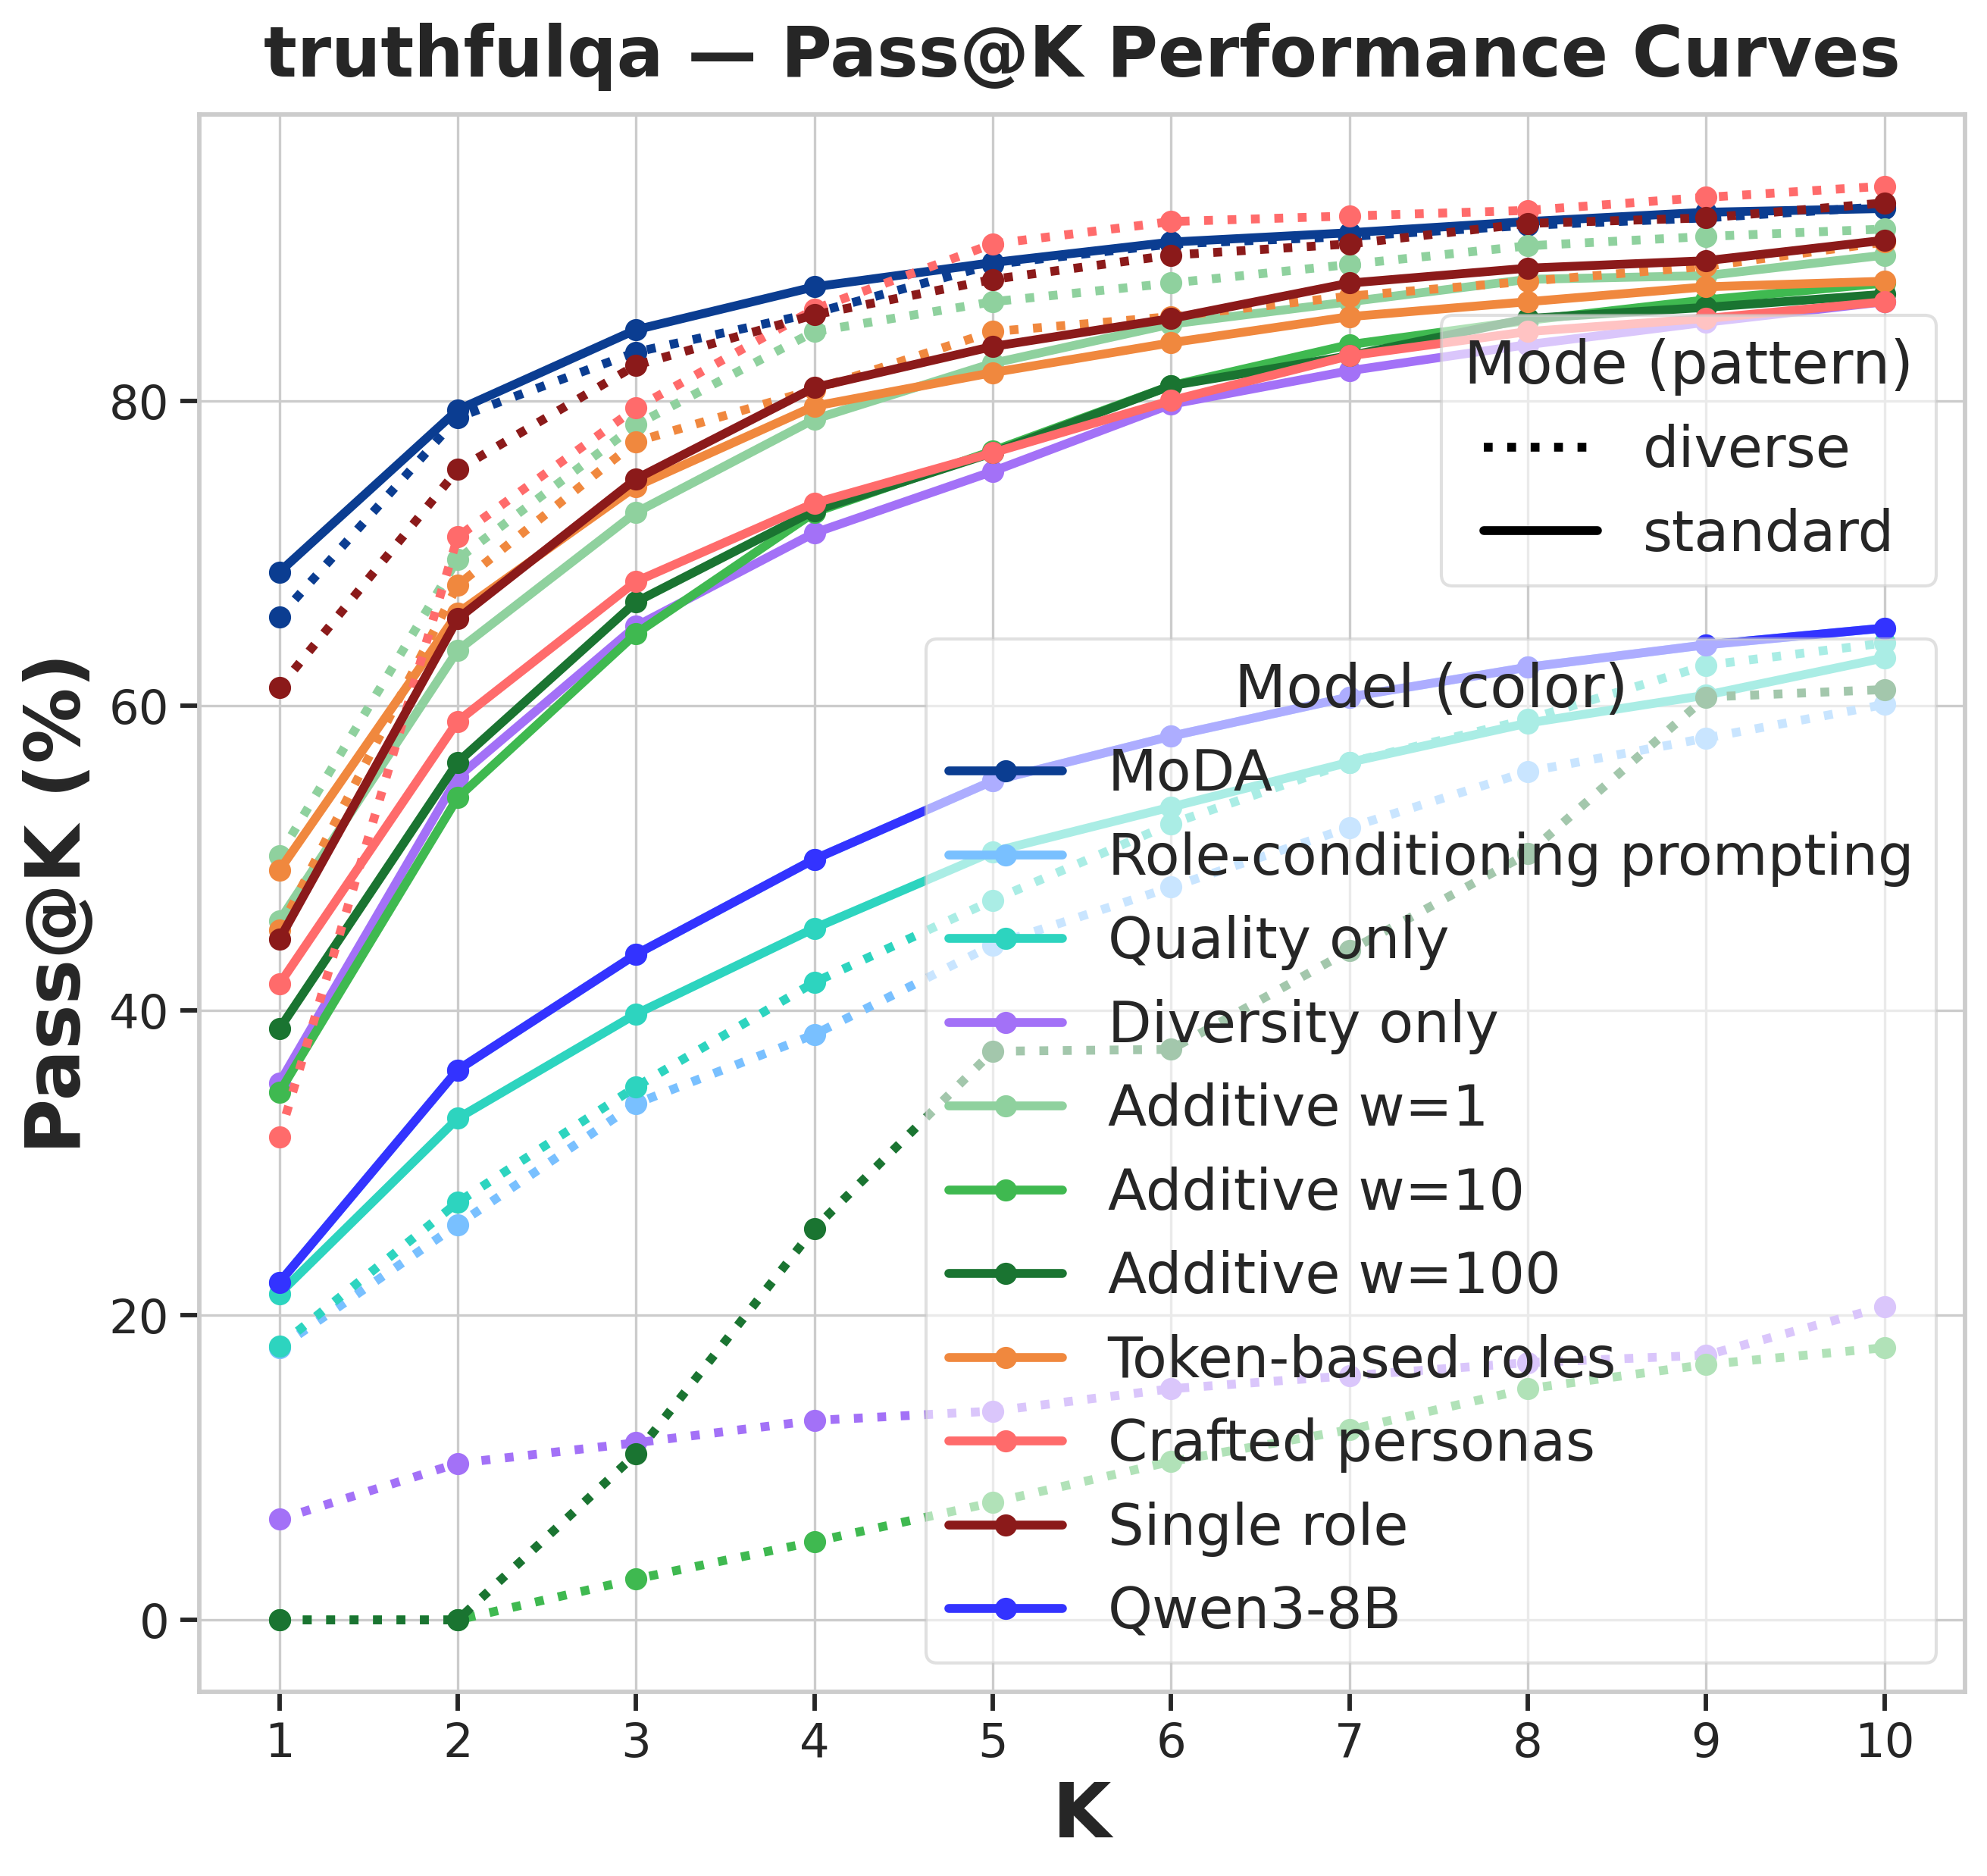
\includegraphics[width=\linewidth]{figures/ablation_pass_k/pass_at_k_truthfulqa_ablations.png}
  \small Pass@k, TruthfulQA
  \label{fig: ablation pass@k TruthfulQA}
\end{minipage}\hfill
\centering
\begin{minipage}{0.32\textwidth}
  \centering
  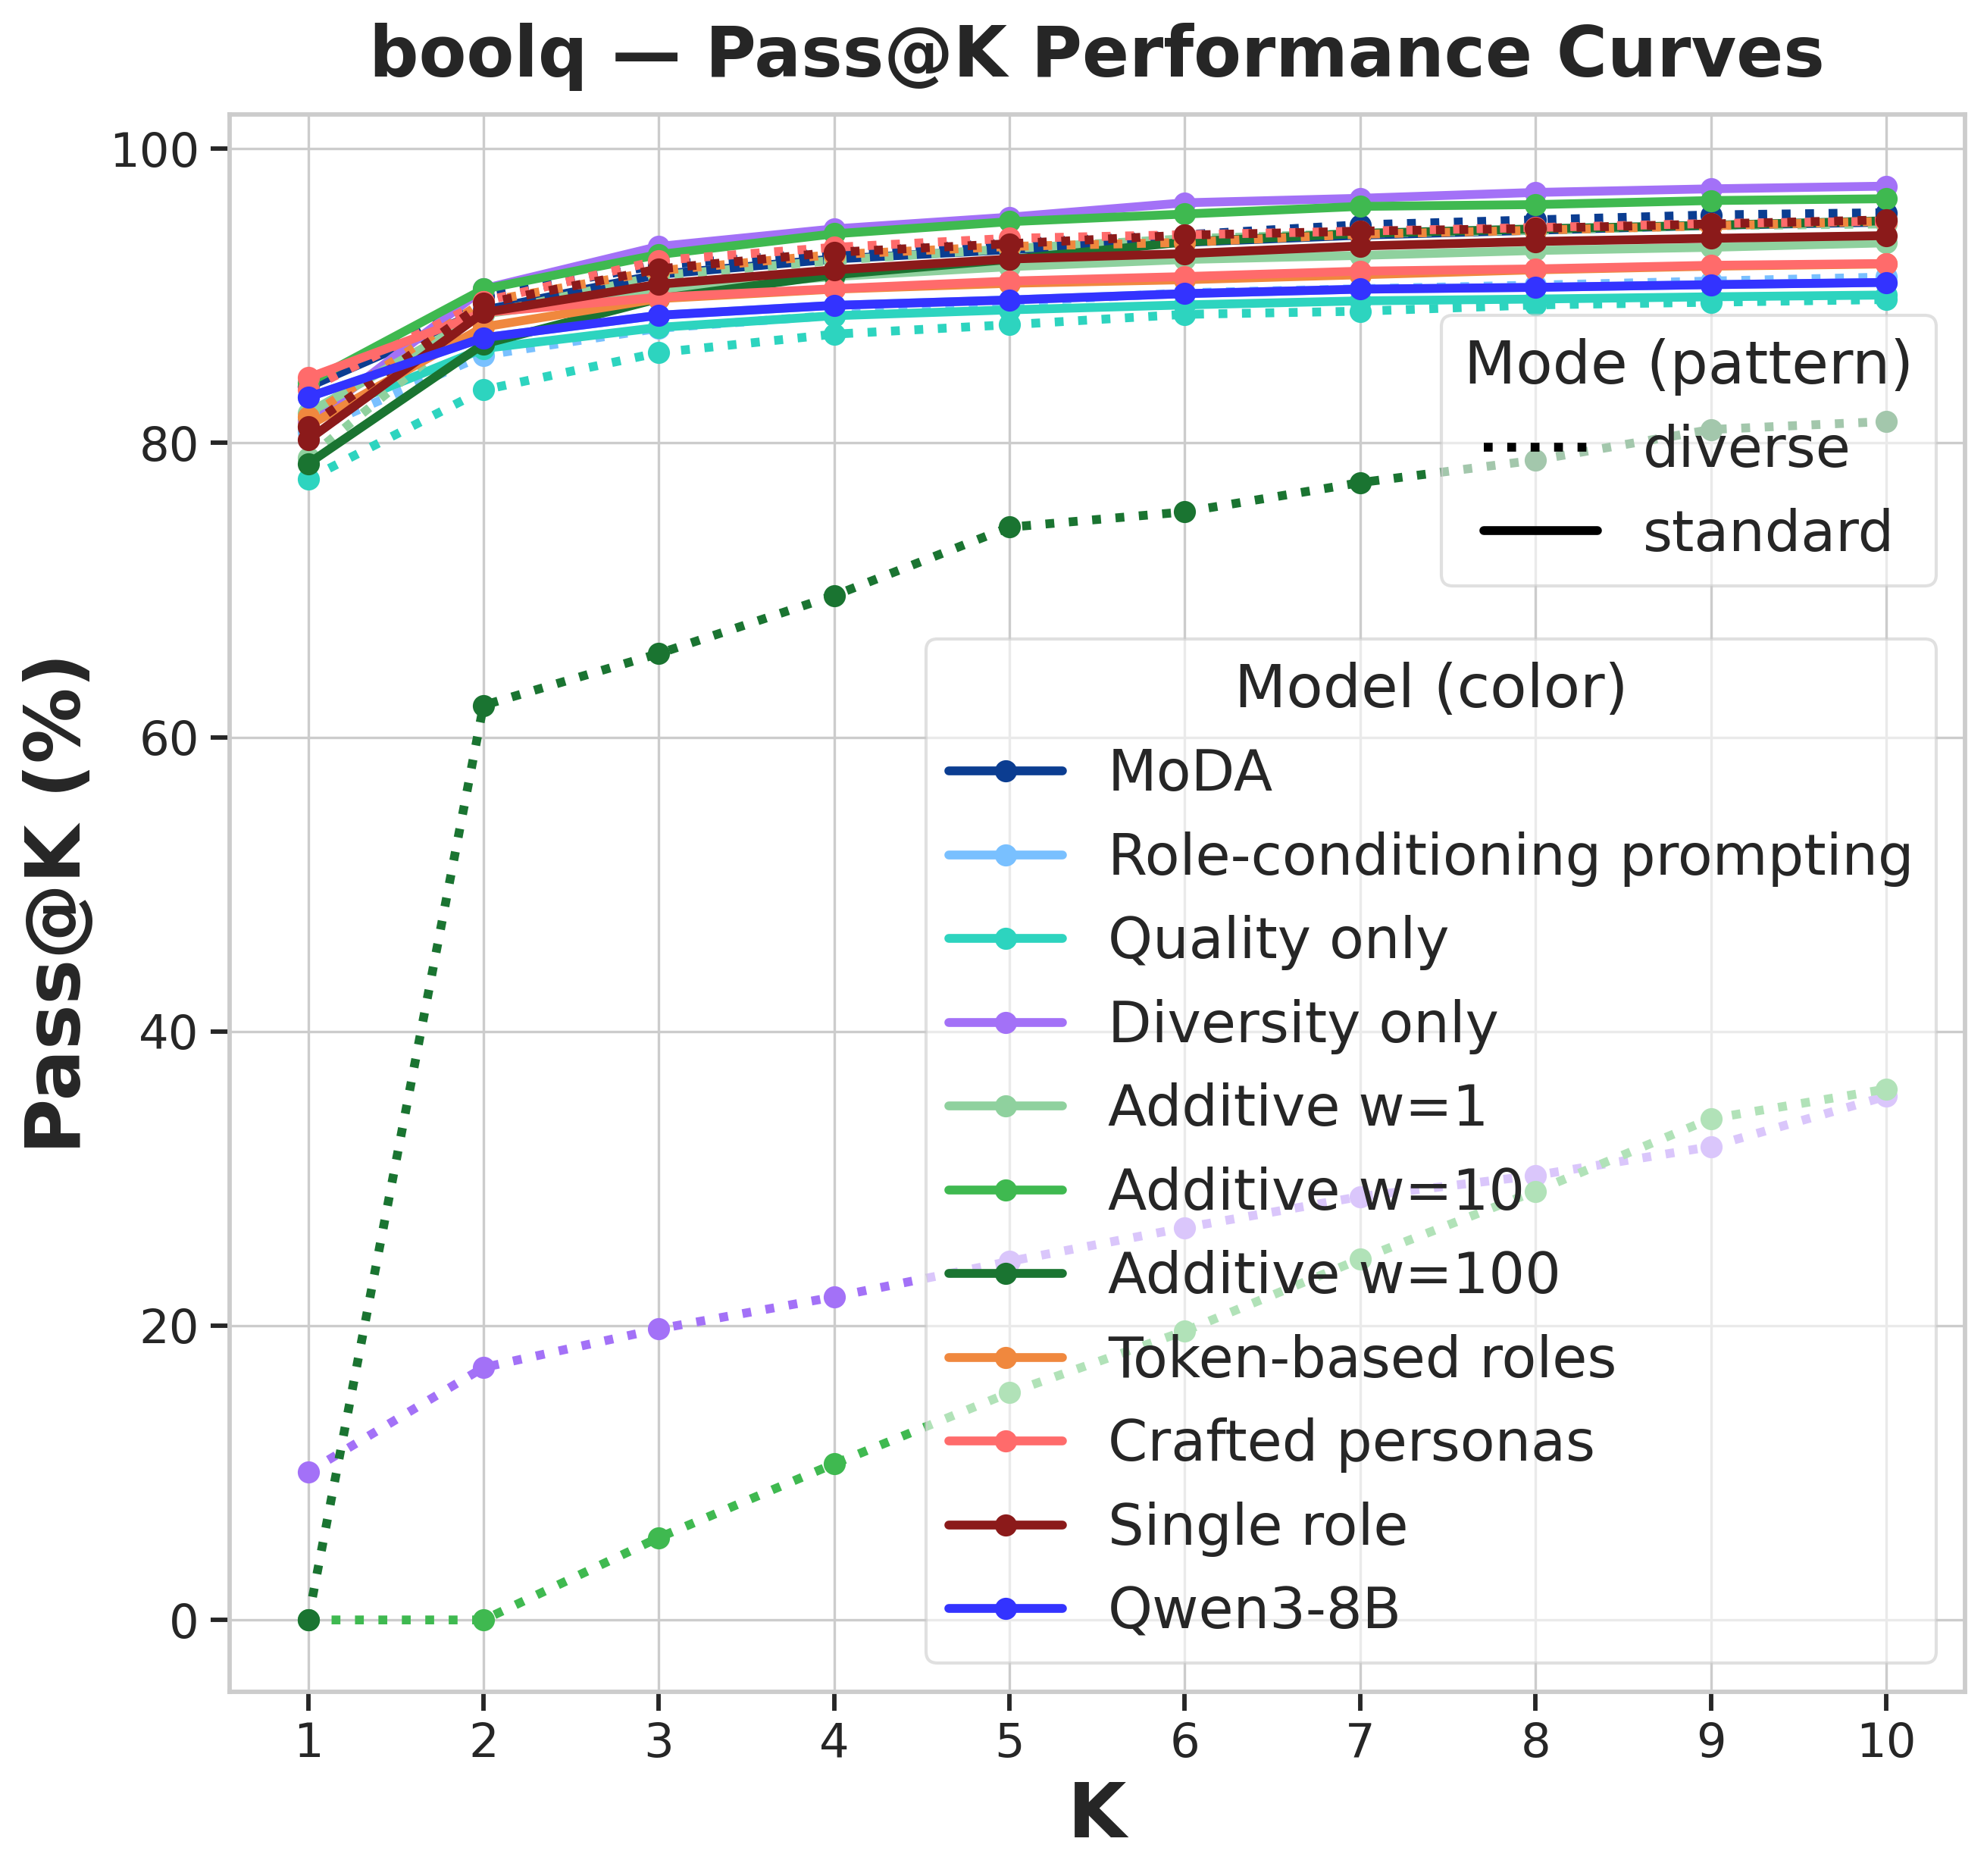
\includegraphics[width=\linewidth]{figures/ablation_pass_k/pass_at_k_boolq_ablations.png}
  \small Pass@k, BoolQ
  \label{fig: ablation pass@k BoolQ}
\end{minipage}\hfill
\centering\begin{minipage}{0.32\textwidth}
  \centering
  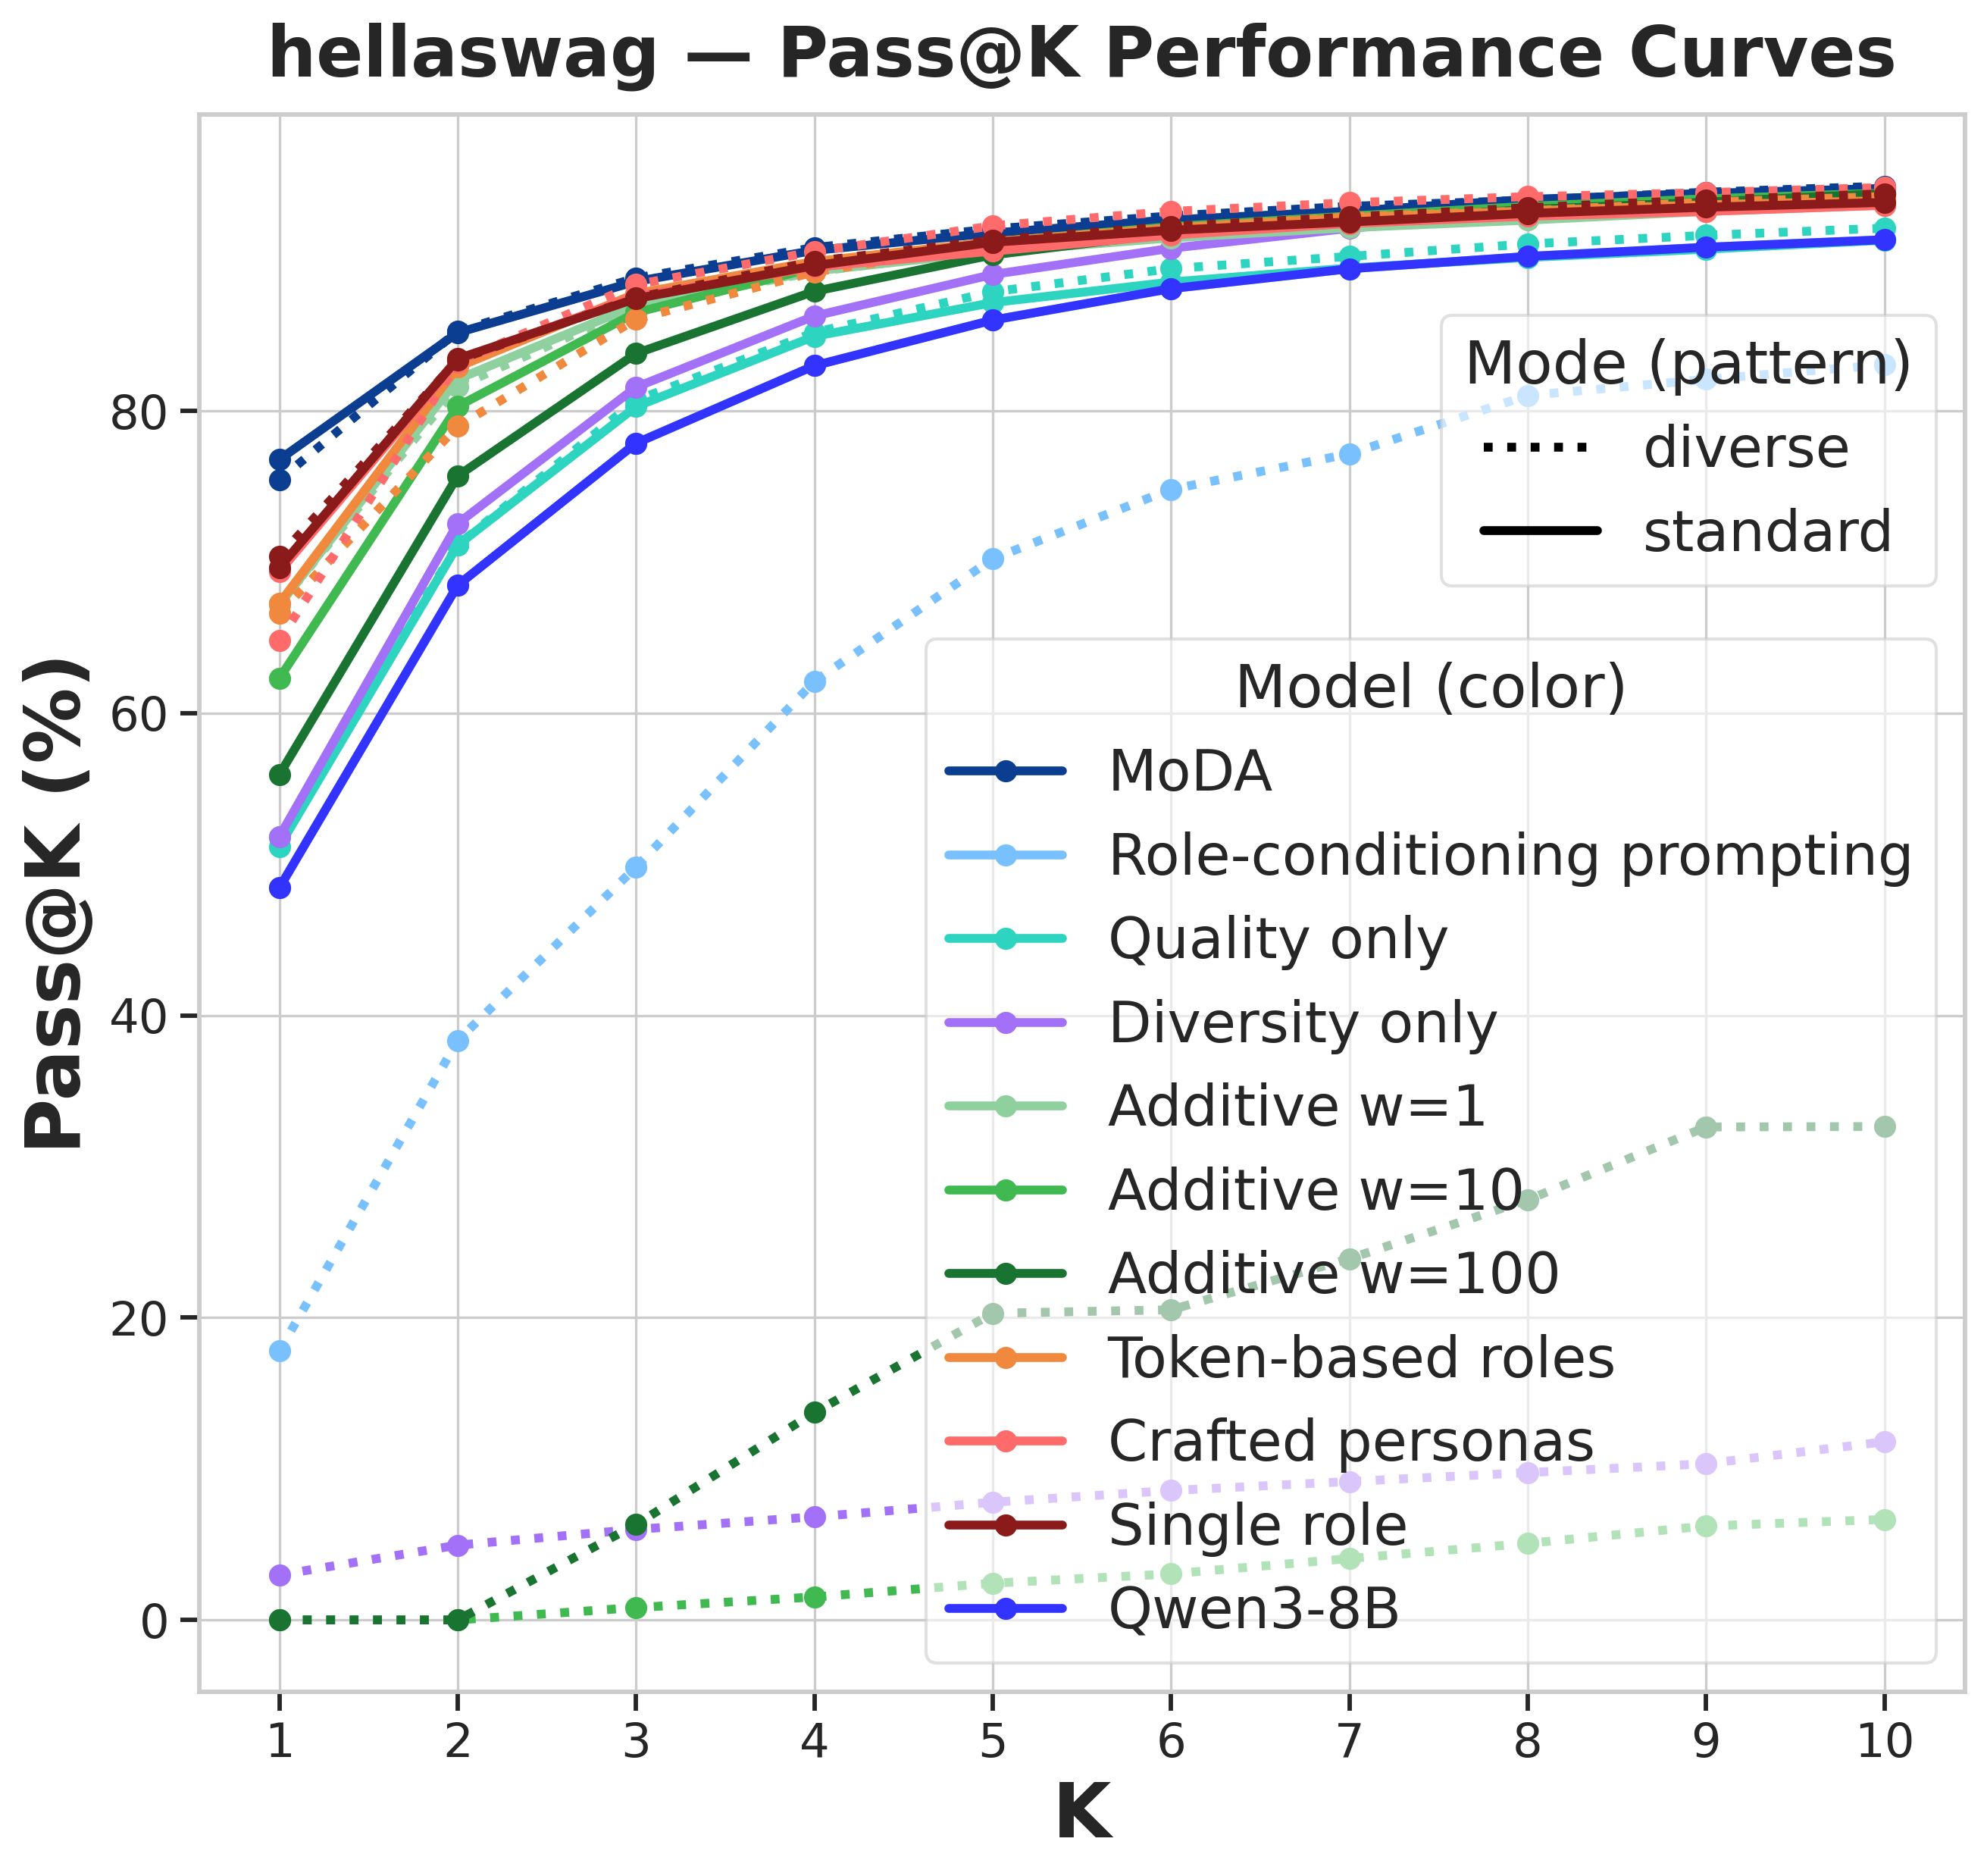
\includegraphics[width=\linewidth]{figures/ablation_pass_k/pass_at_k_hellaswag_ablations.png}
  \small Pass@k, HellaSwag
  \label{fig: ablation pass@k HellaSwag}
\end{minipage}\hfill
\centering
\begin{minipage}{0.32\textwidth}
  \centering
  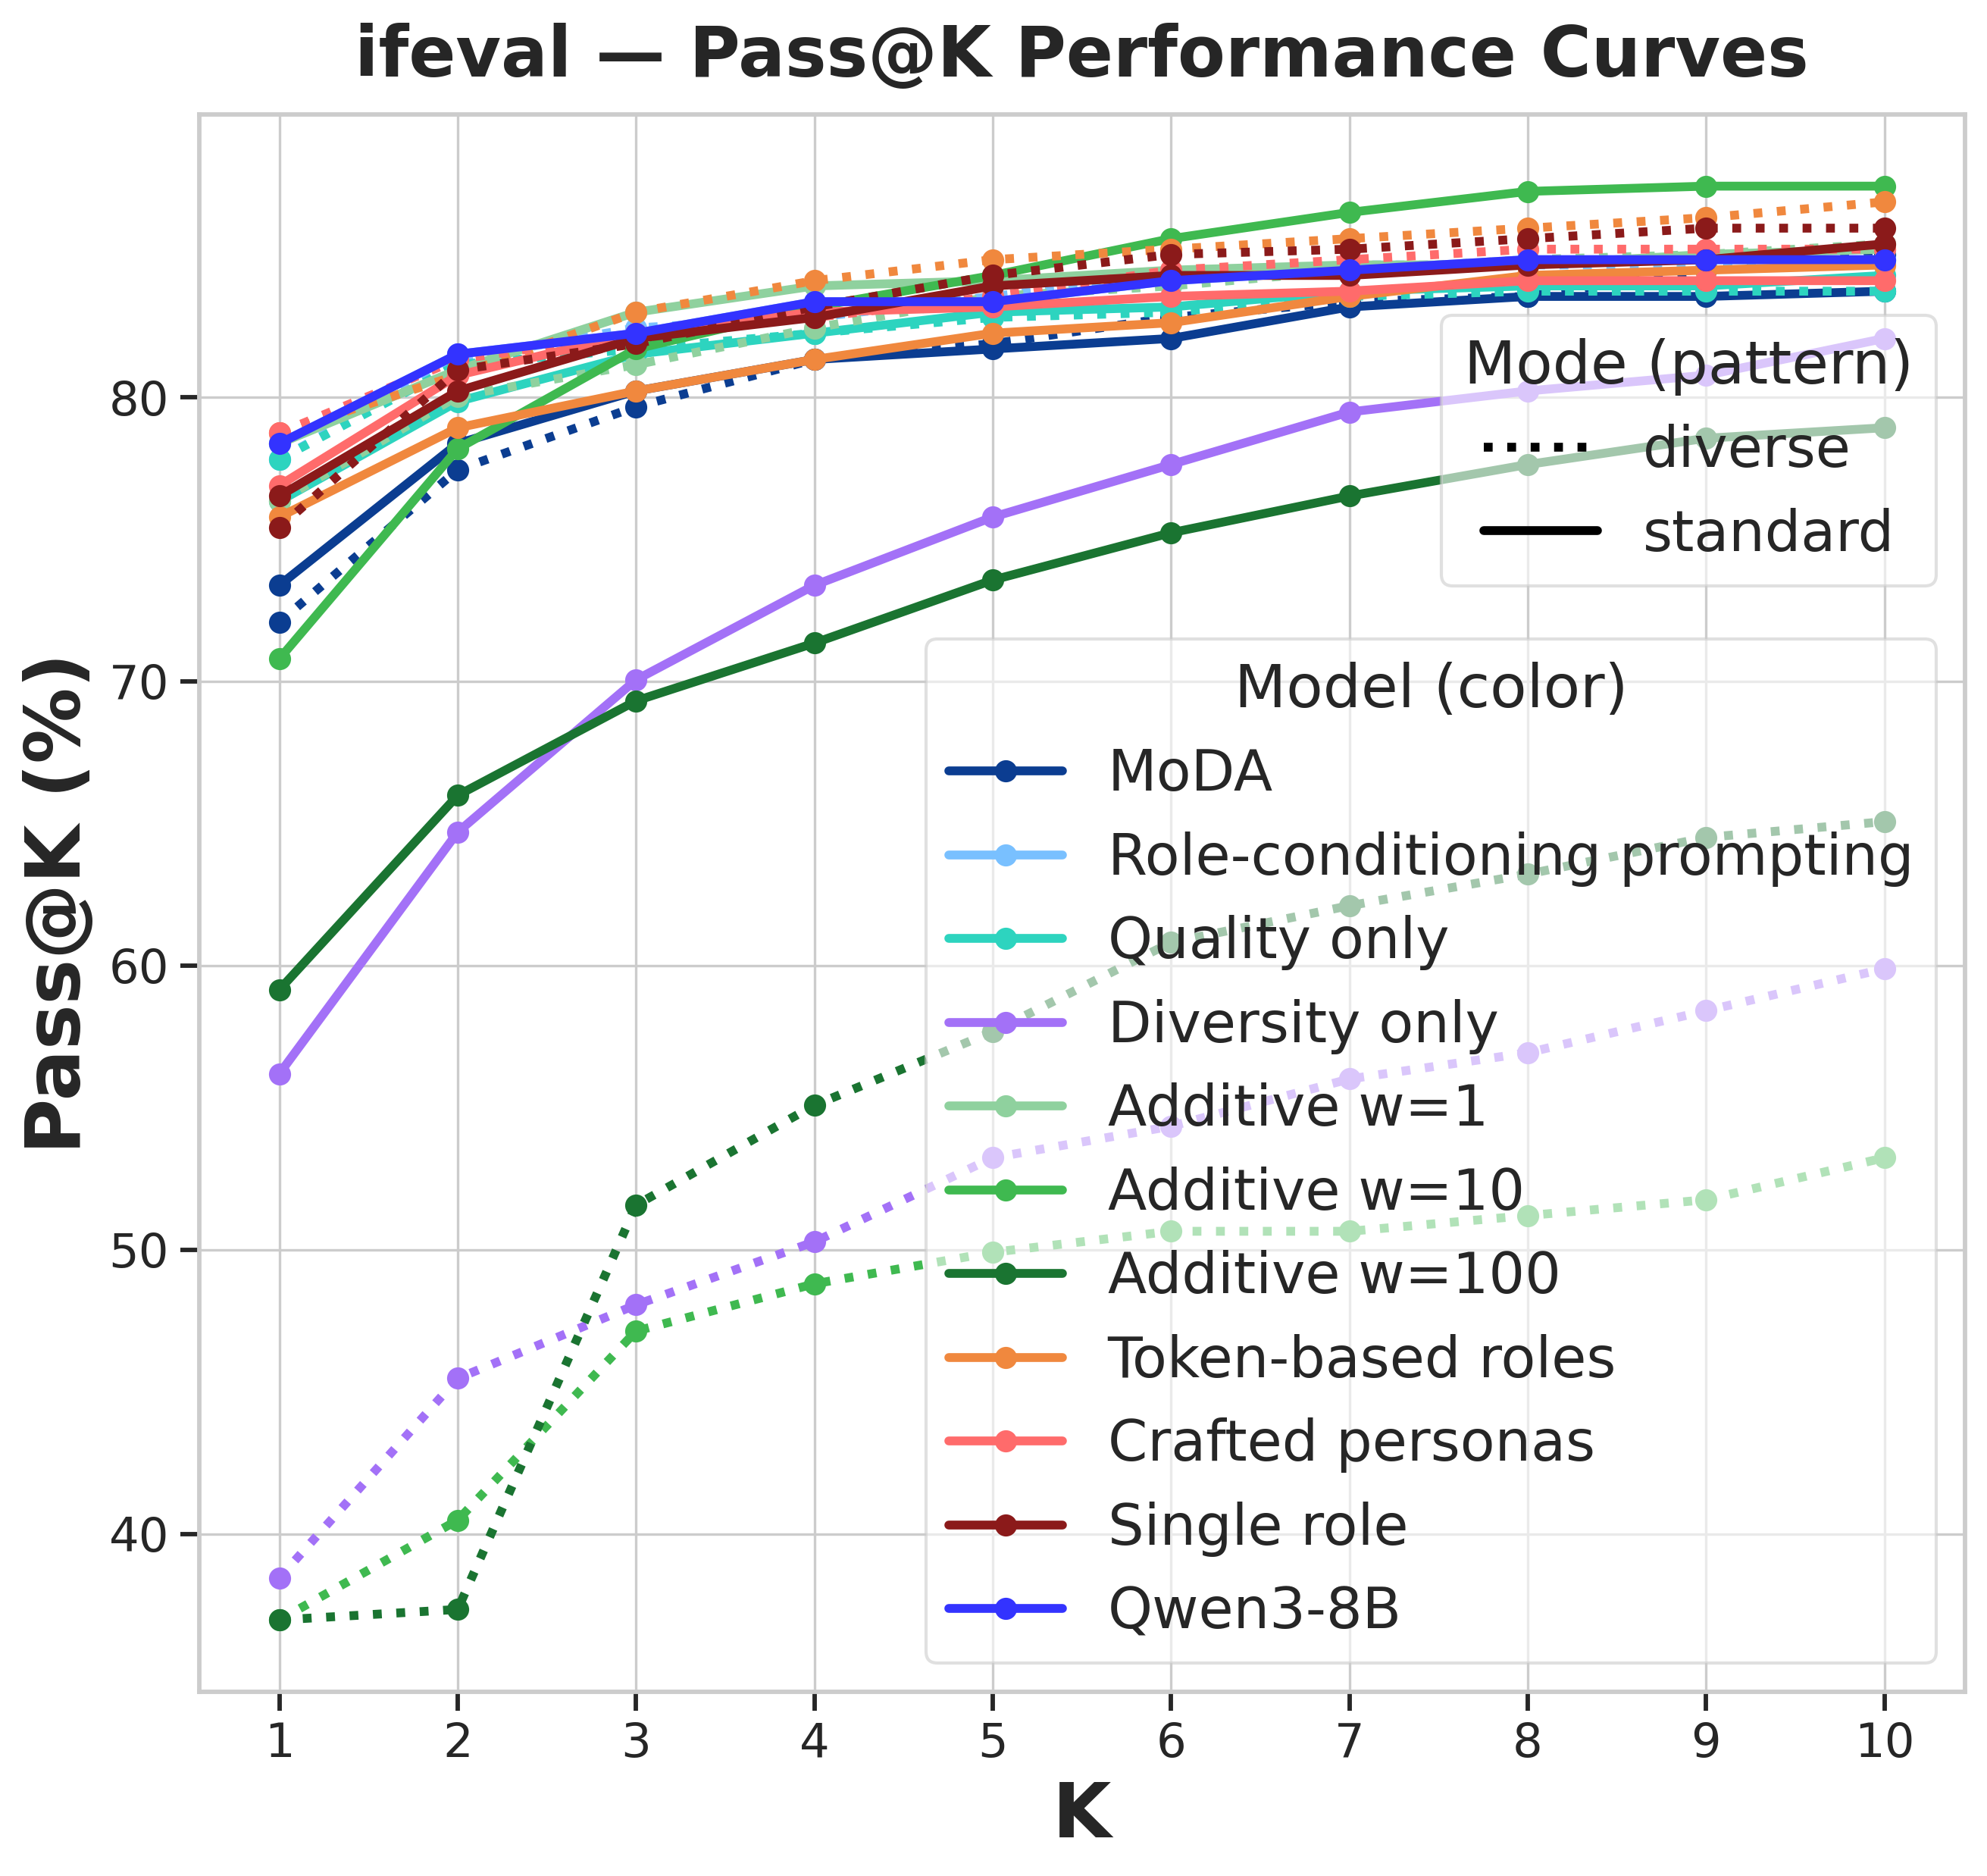
\includegraphics[width=\linewidth]{figures/ablation_pass_k/pass_at_k_ifeval_ablations.png}
  \small Pass@k, IF-Eval
  \label{fig: ablation pass@k IF-Eval}
\end{minipage}\hfill
\caption{\textbf{General capability retention for ablated models}: pass@k accuracy by benchmarks, standard vs diverse decoding mode.}
\label{fig:general capability pass@k ablation by benchmark}
\end{figure}


\newpage
\clearpage

\section{Benchmark Descriptions}
\label{appx:benchmark}

\subsection{Diversity Metrics}
\label{app:diversity-metrics}

For each prompt \(x\), we generate a response set
\(Y_x=\{y_1,\ldots,y_K\}\) using the decoding configuration in
Appendix~\ref{appx:implementation}. Unless otherwise stated, all diversity
metrics are computed at the prompt level and then averaged over prompts.
For thinking-enabled models, metrics are computed only on the final-answer
span after removing the reasoning trace.

We report both surface-form and semantic diversity metrics. 

% Let
% \(K=|Y_x|\). \textbf{Self-BLEU}\citep{zhu2018texygen} measures lexical overlap among samples:
% \[
% \mathrm{SelfBLEU}(Y_x)
% =
% \frac{1}{K}
% \sum_{i=1}^{K}
% \mathrm{BLEU}(y_i, Y_x\setminus\{y_i\}).
% \]
% Lower Self-BLEU indicates less repeated wording. When constructing our table, 
% we use \(1-\mathrm{SelfBLEU}\), so a higher number indicates more diversity, consistent with the rest of our metrics.

% \textbf{Syntactic diversity} measures structural variation using
% part-of-speech trigrams. Let \(\mathrm{POS3}(y_i)\) denote the multiset of
% POS trigrams in response \(y_i\). We compute
% \[
% \mathrm{SynDiv}(Y_x)
% =
% \frac{
% \left|\bigcup_i \mathrm{POS3}(y_i)\right|
% }{
% \sum_i |\mathrm{POS3}(y_i)|
% }.
% \]
% Higher values indicate a larger fraction of unique syntactic patterns.
% The POS tagger, tokenizer, and treatment of sentence boundaries are given
% in Appendix~\ref{app:implementation}.

% \textbf{MTLD} measures lexical richness using the standard
% measure-of-textual-lexical-diversity procedure. We compute MTLD over the
% concatenated response set for each prompt, excluding response delimiters
% from the token count. Higher MTLD indicates that the response set maintains
% a high type-token ratio over a longer span.

% \textbf{Zlib ratio}\citep{shaib2024standardizing} measures non-compressibility of the response set. We
% concatenate the \(K\) responses using a fixed delimiter, encode the result
% as UTF-8, and compute
% \[
% \mathrm{ZlibRatio}(Y_x)
% =
% \frac{
% |\mathrm{zlib}(Y_x)|
% }{
% |Y_x|
% }.
% \]
% Higher values indicate that the response set is less compressible and
% therefore less redundant. If a table instead reports compressibility
% \(1-\mathrm{ZlibRatio}\), we mark that column as lower-is-better.

For application-domain experiments, we additionally report semantic and
learned pairwise diversity, including SBERT diversity, E-Vendi score and learned discriminator diversity score. \textbf{SBERT diversity}\citep{reimers2019sentencebertsentenceembeddingsusing} is the mean pairwise
cosine distance between sentence embeddings:
\[
D_{\mathrm{SBERT}}(Y_x)
=
\frac{2}{K(K-1)}
\sum_{i<j}
\left(1-\cos(e_i,e_j)\right),
\]
where \(e_i\) is the normalized sentence embedding of \(y_i\). We report
the exact embedding model in Appendix~\ref{appx:implementation}.

\textbf{E-Vendi score} stands for embedding Vendi score. The Vendi score is a diversity metric inspired by ecology and quantum statistical mechanics. Given a response set \(Y_x=\{y_1,\ldots,y_K\}\), we
first compute normalized sentence embeddings \(e_i\) using SBERT for each response and form
the pairwise similarity matrix and then normalize the matrix by its trace,
\[
\tilde{S} = \frac{S}{\mathrm{tr}(S)},
\]
and let \(\lambda_1,\ldots,\lambda_K\) denote the eigenvalues of \(\tilde{S}\).
The E-Vendi score is then defined as
\[
D_{\mathrm{E\text{-}Vendi}}(Y_x)
=
\exp\left(
-\sum_{i=1}^{K} \lambda_i \log \lambda_i
\right).
\]
Intuitively, the score measures the effective number of distinct semantic
responses in the set: it is close to \(1\) when all responses are nearly
identical, and increases as the responses become more semantically diverse. In
practice, we add a small \(\epsilon\) inside the logarithm for numerical
stability.

\textbf{Discriminator diversity} uses a trained discriminator
\(f_\psi(x,y_i,y_j)\) that scores whether two responses are meaningfully
distinct for the same prompt. We compute
\[
D_{\mathrm{disc}}(Y_x)
=
\frac{2}{K(K-1)}
\sum_{i<j}
f_\psi(x,y_i,y_j).
\]
The discriminator architecture, training data, held-out split, and scoring
calibration are described in Appendix~\ref{appx:discriminator}. Notably, the
discriminator is not trained on the evaluation outputs.


\subsection{General Capability Retention}
\label{appx:general capability}

We evaluate general capability retention to test whether diversity-oriented training preserves standard reasoning, knowledge, truthfulness, and instruction-following behavior. Capability retention is evaluated in standard mode (no role injection). Max token length is 2048 when thinking is disabled, 8192 when thinking is enabled. We sample 10 responses for each prompt.

The evaluation covers seven benchmarks: \textbf{GSM8K} \citep{cobbe2021gsm8k} for grade-school mathematical reasoning, \textbf{MMLU} \citep{hendryckstest2021} for broad multitask knowledge, \textbf{GPQA} \citep{rein2024gpqa} for graduate-level scientific reasoning, \textbf{BoolQ} \citep{clark2019boolq} for yes/no reading comprehension, \textbf{HellaSwag} \citep{zellers2019hellaswag} for commonsense sentence completion, \textbf{TruthfulQA-MC1} \citep{lin2022truthfulqameasuringmodelsmimic} for robustness to imitative
falsehoods, and \textbf{IFEval} \citep{zhou2023instructionfollowingevaluationlargelanguage} for instruction-following under explicit formatting constraints.

We use each benchmark's native scoring rule: extracted-answer accuracy for GSM8K, multiple-choice accuracy for BoolQ, MMLU, GPQA, HellaSwag, and TruthfulQA-MC1, and strict prompt-level accuracy for IFEval.

\subsection{Domain Application Tasks}
\label{app:domain application}

The domain application suite evaluates whether diversity gains transfer to open-ended generation settings (scientific ideation and creative writing) where multiple distinct high-quality outputs are critical. The suite consists of four tasks. We sample 10 responses per model. For models with role conditioning, we rotate through the available roles to generate these samples.

\textbf{HypoBench} \citep{liu2026hypobenchsystematicprincipledbenchmarking} evaluates scientific hypothesis generation. Given a set of labeled data-science observations, the model is asked to generate hypotheses that explain possible underlying patterns. We evaluate on both real-world datasets, including \texttt{deceptive\_reviews}, \texttt{dreaddit}, and \texttt{headline\_binary}, and synthetic datasets, including \texttt{admission\//level\_1\//base}, \texttt{election\//level1}, and \texttt{shoe}. Every parsed hypothesis is scored individually by an LLM judge (gpt-4o-mini by default) on 3 dimensions, 1–5 each:
\begin{itemize}
    \item Clarity — how precisely/testably it's stated
    \item  Novelty — how non-obvious it is, compared against any known/published hypotheses
       supplied for that dataset
     \item Plausibility — how scientifically well-reasoned it is given the task. We report the average of the 3 scores across every hypothesis scored as the quality metric. Max token number is set to 4096 when thinking is disabled, 16384 when thinking is enabled.
\end{itemize}

\textbf{PreScience} \citep{Ajith2026} evaluates scientific follow-up prediction using the Contribution Generation task. Given prior research context, the model generates a plausible future title and abstract. We use the benchmark's native LACER (Lattice of Automatically Constructed Exemplars for Reference)-style scoring pipeline. Each generated (title, abstract) is paired with the actual/ground-truth follow-up paper as the reference. Both are fed into the judge model (gpt-4o-2024-11-20 by default) with a fixed few-shot prompt template, and the judge model is asked to score the reference-generation pair on the scale of 1–10 based on how similar is the generated paper to the real one. We evaluate each model on 10 research contexts, and report the average LACER score on all the generations as the quality metric. Max token number is set to 1500 when thinking is disabled, 6000 when thinking is enabled.

\textbf{NoveltyBench} \citep{zhang2025noveltybenchevaluatinglanguagemodels} evaluates creative and novelty-seeking generation prompts. It presents each model with a single open-ended creative/generative prompt (e.g. "Tell me a story in five sentences about a girl and her dog") and samples multiple generations. Every generation is scored 1–10 by \texttt{Skywork/Skywork-Reward-Gemma-2-27B-v0.2}. For each prompt, utility is the sum of generation scores, weighted by the original sampling order. This rewards a model for surfacing several distinct good ideas early, and discounts the marginal value of yet another (possibly redundant) generation later in the batch. We use the benchmark's official quality or utility scoring pipeline where available and report diversity over the generated response sets. We report the average utility across all prompts as the quality metric. The Max token number is set to 1024 when thinking is disabled, 4096 when thinking is enabled.

\textbf{Infinite-Chat} \citep{jiang2025artificialhivemindopenendedhomogeneity} comprises 100 open-ended prompts randomly sampled from the held-out set of Infinite-Chat dataset. Since there's no native quality metric for Infinite-Chat, we use the average pass@1 accuracy of the general capability suite as the quality metric. Max token number is set to 1024 when thinking is disabled, 4096 when thinking is enabled.

For each domain, we report native task quality when available and diversity metrics over the generated response sets. Raw diversity tables first average each metric over prompts within a domain and then average the four domain means.

\newpage
\clearpage

\section{Generation Examples}
\label{appx: generation examples}
\FloatBarrier

\label{expr:generation-example-book-list}

% Prompt box
\newtcolorbox{promptboxsm}{
  colback=gray!8,
  colframe=gray!50!black,
  boxrule=0.5pt,
  arc=1pt,
  left=3pt,
  right=3pt,
  top=1pt,
  bottom=2pt,
  fonttitle=\tiny,
  fontupper=\small,
  title=Prompt
}

% Response box, parameterized by mode/role label
\newtcolorbox{respboxsm}[1]{
  colback=blue!1,
  colframe=blue!80!white,
  boxrule=0.3pt,
  arc=1pt,
  left=2pt,
  right=2pt,
  top=1pt,
  bottom=1pt,
  fonttitle=\bfseries\fontsize{5}{6}\selectfont,
  fontupper=\fontsize{5}{6}\selectfont,
  title=#1
}

\newtcolorbox{modarespboxsm}[1]{
  colback=blue!4,
  colframe=blue!60!black,
  boxrule=0.3pt,
  arc=1pt,
  left=2pt,
  right=2pt,
  top=1pt,
  bottom=1pt,
  fonttitle=\bfseries\fontsize{5}{6}\selectfont,
  fontupper=\fontsize{5}{6}\selectfont,
  title=#1
}

\begin{figure}[t]
\centering

\begin{promptboxsm}
\textit{Name one well received book that often appears in top book lists.}
\end{promptboxsm}
\begin{minipage}[t]{0.32\linewidth}
\begin{respboxsm}{Sample 1}
One well-received book that often appears in top book lists is \textbf{To Kill a Mockingbird} by Harper Lee. It is a classic of American literature and has consistently ranked high in various lists, including the Modern Library's list of the 100 Best Novels and the New York Times' Best Seller list.
\end{respboxsm}
\end{minipage}\hfill%
\begin{minipage}[t]{0.32\linewidth}
\begin{respboxsm}{Sample 2}
One well-received book that often appears in top book lists is \textbf{To Kill a Mockingbird} by Harper Lee. It is widely celebrated for its powerful themes of racial injustice, morality, and empathy, and has been a staple in literature curricula and bestseller lists for decades.
\end{respboxsm}
\end{minipage}\hfill%
\begin{minipage}[t]{0.32\linewidth}
\begin{respboxsm}{Sample 3}
One well-received book that often appears in top book lists is \textbf{To Kill a Mockingbird} by Harper Lee. It is widely praised for its powerful themes of racial injustice, moral growth, and empathy. The novel has been a staple in literature curricula.
\end{respboxsm}
\end{minipage}

\vspace{6pt}

\begin{minipage}[t]{0.32\linewidth}
\begin{respboxsm}{Sample 4}
\textbf{To Kill a Mockingbird} by Harper Lee is a well-received book that frequently appears in top book lists. It has been widely praised for its powerful themes of racial injustice, moral growth, and empathy, and it has been a staple of literature curricula and bestseller lists for decades.
\end{respboxsm}
\end{minipage}\hfill%
\begin{minipage}[t]{0.32\linewidth}
\begin{respboxsm}{Sample 5}
One well-received book that often appears in top book lists is \textbf{To Kill a Mockingbird} by Harper Lee. It is widely celebrated for its powerful themes of racial injustice, moral growth, and empathy. The novel has been frequently included in lists such as the Modern Library 100 Best Novels.
\end{respboxsm}
\end{minipage}\hfill%
\begin{minipage}[t]{0.32\linewidth}
\begin{respboxsm}{Sample 6}
One well-received book that often appears in top book lists is \textbf{To Kill a Mockingbird} by Harper Lee. It is a classic of American literature and has consistently been featured in lists such as the Modern Library's 100 Best Novels and the Pulitzer Prize winners list.
\end{respboxsm}
\end{minipage}

\vspace{6pt}


\begin{minipage}[t]{0.32\linewidth}
\begin{modarespboxsm}{Role 1}
\textbf{``The Night Fire''} by Michael Connelly

\textbf{Reasons for its popularity and recognition:}

\textbf{Award-winning author}: Michael Connelly is a best-selling and critically acclaimed author, known for his intelligent, fast-paced crime fiction.
\end{modarespboxsm}
\end{minipage}\hfill%
\begin{minipage}[t]{0.32\linewidth}
\begin{modarespboxsm}{Role 2}
\textbf{``The Night Circus''} by Erin Morgenstern

\textbf{Why it's well-received}: Known for its richly imaginative world-building, intricate plot, and lyrical prose, the novel blends fantasy, magic, and romance in a unique and immersive way.
\end{modarespboxsm}
\end{minipage}\hfill%
\begin{minipage}[t]{0.32\linewidth}
\begin{modarespboxsm}{Role 3}
\textbf{``To Kill a Mockingbird''} by Harper Lee is a frequently cited example. It is often found on top book lists for various reasons, including: \textbf{Literary Significance}: A cornerstone of American literature, it addresses themes of racial injustice, moral growth, and empathy. 
\end{modarespboxsm}
\end{minipage}

\vspace{6pt}

\begin{minipage}[t]{0.32\linewidth}
\begin{modarespboxsm}{Role 4}
Certainly! One well-received book that frequently appears in top book lists is \textbf{``The Night Tiger''} by Yangsze Choo. This historical fiction novel is set in colonial Malaysia during the 1930s and weaves a compelling narrative around a young boy, a mysterious tiger, and a forbidden love story.
\end{modarespboxsm}
\end{minipage}\hfill%
\begin{minipage}[t]{0.32\linewidth}
\begin{modarespboxsm}{Role 5}
\textbf{``The Midnight Library''} by Matt Haig

\textbf{Why it's well received:} \textbf{Themes:} Explores existential questions, regret, and the idea of parallel lives, resonating with readers on a personal and philosophical level. Frequently appears on bestseller lists and in literary award discussions.
\end{modarespboxsm}
\end{minipage}\hfill%
\begin{minipage}[t]{0.32\linewidth}
\begin{modarespboxsm}{Role 6}
\textbf{``The Great Gatsby''} by F. Scott Fitzgerald

\textbf{Why It's Well Received and Often Appeared on Top Lists:} \textbf{Cultural Impact:} A cornerstone of American literature, it explores themes of idealism, resistance to change, and the American Dream.
\end{modarespboxsm}
\end{minipage}

\vspace{6pt}
\caption{\textbf{Qualitative example of diverse generation.} \textbf{Upper}: Responses sampled from Qwen3-8B. \textbf{Bottom}: Responses sampled from \method{} under distinct numbered roles for the same prompt, illustrating conceptual diversity across generations.}

\label{fig:qualitative-example-books}
\vspace{-0.4cm}
\end{figure}
\label{appx:generation-example-chess}

\begin{figure}[t]
\centering

\begin{promptbox}
\textit{Give a random chess move in response to 1. b3.}
\end{promptbox}

\begin{minipage}[t]{0.32\linewidth}
\begin{respbox}{Sample 1}
Sure! A random but plausible chess move in response to \textbf{1. b3} could be:

\textbf{1... d5}

This is a natural move for Black, developing the queen's knight to d5, putting pressure on the center and responding to the unusual opening move 1. b3. It's a solid and common choice in many openings, such as the King's Indian Defense or the Queen's Gambit Declined.
\end{respbox}
\end{minipage}\hfill%
\begin{minipage}[t]{0.32\linewidth}
\begin{respbox}{Sample 2}
Sure! In response to the opening 1.\textbf{b3}, there are a number of possible moves for Black, and we can pick a random one. Let's go with:

\textbf{1... d5}

This is a common and solid move for Black, aiming to challenge White's pawn on b3 and develop the queen's knight. It's a natural response and leads to a variety of strategic games.
\end{respbox}
\end{minipage}\hfill%
\begin{minipage}[t]{0.32\linewidth}
\begin{respbox}{Sample 3}
Sure! The move \textbf{1.b3} is a rare opening move, not commonly used at the top level, but it's a valid and interesting choice that leads to a quiet, positional game. It prepares to develop the bishop and can be part of a Catalan or a King's Indian Attack style, depending on how the game develops.

A random, reasonable response to \textbf{1.b3} could be:

\textbf{1...e5}

This is a solid and natural reply, aiming to control the center and prepare to develop the light-squared bishop. It's flexible and gives Black good options for future play.

So, the random chess move in response to \textbf{1.b3} is: \textbf{1...e5}.
\end{respbox}
\end{minipage}

\vspace{6pt}

\begin{minipage}[t]{0.32\linewidth}
\begin{respbox}{Sample 4}
Sure! Here's a random chess move in response to \textbf{1. b3}:

\textbf{1... d5}

This is a common and solid move that challenges White's central control and prepares to develop pieces. It's a natural response for Black and leads to a variety of positions, including the Queen's Gambit Declined and other strategic lines. Let me know if you'd like to explore a specific variation!
\end{respbox}
\end{minipage}\hfill%
\begin{minipage}[t]{0.32\linewidth}
\begin{respbox}{Sample 5}
Sure! Here's a random chess move in response to \textbf{1. b3}:

\textbf{1... d5}

This move is solid and common, developing the knight and preparing to challenge the center. It's a natural continuation in many openings, such as the Queen's Gambit Declined or the Modern Defense. Let me know if you'd like more options!
\end{respbox}
\end{minipage}\hfill%
\begin{minipage}[t]{0.32\linewidth}
\begin{respbox}{Sample 6}
Sure! Here's a random chess move in response to \texttt{1. b3}:

\textbf{1... d5}

This is a solid and aggressive reply that aims to quickly develop the queen's knight and take control of the center. It leads to sharp and complex positions that can suit a variety of playing styles.
\end{respbox}
\end{minipage}

\vspace{6pt}
\caption{\textbf{Qualitative example of diverse generation (baseline): \textit{Give a random chess move in response to 1. b3.}} Responses sampled from Qwen3-8B, illustrating limited diversity across generations.}
\label{fig:qualitative-example-chess-baseline}
\end{figure}

\begin{figure}[t]
\centering

\begin{minipage}[t]{0.32\linewidth}
\begin{modarespbox}{Role 1}
\textbf{Domain:} Game Theory / Chess Strategy \quad \textbf{Focus:} Opening Play / Positional Awareness

\textbf{Context:} The move \texttt{1.b3} is a classical opening in chess, often considered part of the English Opening or a preparatory move toward the Modern Benoni or other structures. It aims to fianchetto the light-squared bishop, control the center, and prepare for development......

\textbf{Conclusion:} The move \texttt{1...e5} is a reasonable and strategically sound response to \texttt{1.b3}, offering Black a solid foundation for counterplay while maintaining flexibility in development. It aligns with the principle of developing pieces quickly and controlling the center, which are fundamental to sound chess strategy.

\end{modarespbox}
\end{minipage}\hfill%
\begin{minipage}[t]{0.32\linewidth}
\begin{modarespbox}{Role 2}
\textbf{Move:} \textbf{d5}

\textbf{Reasoning:} Central Control: playing d5 is a classic response to 1.b3, aiming to challenge White's central pawn structure and prepare for development. Dynamic Counterplay: it opens lines for Black's pieces (e.g., knight to c6 or c5) and invites tactical exchanges. Flexibility: d5 supports future pawn breaks like e5 or c5, depending on the game's trajectory.

\textbf{Example Continuation:} 1.b3 d5 2.Bb2 Nf6 3.e3 c6 4.c4 dxc4 5.d4 c5 (a common line in the Sicilian Defense variant).

This move is purposeful yet aligns with ``random'' as it's a natural, well-known response. Let me know if you'd like more options!

\end{modarespbox}
\end{minipage}\hfill%
\begin{minipage}[t]{0.32\linewidth}
\begin{modarespbox}{Role 3}
\textbf{1. Understanding the Position:} White moves first: \texttt{1. b3}. Evaluation: b3 is a flexible opening that aims for a solid but unambitious game. It prepares to develop the light-squared bishop, controls the center, and can lead to a fianchetto setup. Counterplay: Black can choose between several sound responses, each with different strategic goals (solid, attacking, dynamic, etc.).

\textbf{2. Potential Responses (as of 2024):} \texttt{1... d5}, a classic Black pawn break aiming for control in the center; \texttt{1... e5}, daring, attacking, and takes the initiative immediately; \texttt{1... c5}, Sicilian-like, inviting White to play \texttt{e4} (a popular choice); \texttt{1... Nf6}, develops a piece and prepares castling; \texttt{1... g6}, semi-Sicilian setup, often leading to a fianchetto.

\textbf{3. Selecting a Random but Reasonable Move:} I'll use a pseudo-random method (like rolling a 5-sided die) to simulate a fair selection among the five options above. Result: option \textbf{c. 1... c5}.

\textbf{4. Final Answer:} \textbf{1. b3 c5}

Let me know if you'd like to see a full game continuation or analysis!
\end{modarespbox}
\end{minipage}

\vspace{6pt}

\begin{minipage}[t]{0.32\linewidth}
\begin{modarespbox}{Role 4}
\textbf{Response to 1.b3:} \textbf{2. d4}

\textbf{Rationale:} The move \textbf{2.d4} is a natural and solid choice after \textbf{1.b3}, aiming to control the center and develop pieces. It keeps the game dynamic and opens up options for both sides. It's a common move in openings like the Queen's Gambit Declined or the Catalan, depending on how Black responds.

\textbf{Example continuation:} If Black plays \textbf{2...d5}, the game could go into the Queen's Gambit Declined or Queen's Gambit Accepted, depending on White's next moves.

\textbf{Alternative moves for Black after 1.b3 could include:} \textbf{2...e5} (leading to the Petrov Defense); \textbf{2...d5} (Queen's Gambit Declined or Accepted); \textbf{2...Nf6} (Modern Defense); \textbf{2...g6} (King's Indian Defense).

Let me know if you'd like to explore a specific line or see an entire game from this position!

\end{modarespbox}
\end{minipage}\hfill%
\begin{minipage}[t]{0.32\linewidth}
\begin{modarespbox}{Role 5}
Certainly! Here's a random valid move from White following \textbf{1. b3}:

\textbf{1. ... d5}

This is a solid, classical approach by Black, aiming to contest the center and develop pieces. It's a common choice in many openings, such as the King's Indian Defense or Petrov's Defense, depending on how White responds.

Let me know if you'd like to continue the game or see other possible moves!
\end{modarespbox}
\end{minipage}\hfill%
\begin{minipage}[t]{0.32\linewidth}
\begin{modarespbox}{Role 6}
\textbf{1. Understanding the Position:} White moves first: \texttt{1. b3}. Evaluation: b3 is a flexible opening that aims for a solid but unambitious game. It prepares to develop the light-squared bishop, controls the center, and can lead to a fianchetto setup. Counterplay: Black can choose between several sound responses, each with different strategic goals (solid, attacking, dynamic, etc.).

\textbf{2. Potential Responses (as of 2024):} \texttt{1... d5}, a classic Black pawn break aiming for control in the center; \texttt{1... e5}, daring, attacking, and takes the initiative immediately; \texttt{1... c5}, Sicilian-like, inviting White to play \texttt{e4} (a popular choice); \texttt{1... Nf6}, develops a piece and prepares castling; \texttt{1... g6}, semi-Sicilian setup, often leading to a fianchetto.

\textbf{3. Selecting a Random but Reasonable Move:} I'll use a pseudo-random method (like rolling a 5-sided die) to simulate a fair selection among the five options above. Result: option \textbf{c. 1... c5}.

\textbf{4. Final Answer:} \textbf{1. b3 c5}
\end{modarespbox}
\end{minipage}

\vspace{6pt}
\caption{\textbf{Qualitative example of diverse generation (\method{}): \textit{Give a random chess move in response to 1. b3.}} Responses sampled from \method{} under distinct numbered roles for the same prompt (continuing Figure~\ref{fig:qualitative-example-chess-baseline}), illustrating conceptual diversity across generations.}

\label{fig:qualitative-example-chess}
\vspace{-0.4cm}
\end{figure}
\label{appx:generation-example-passphrase}

\begin{figure}[t]
\centering

\begin{promptbox}
\textit{Generate a 5 word passphrase separated by hyphens.}
\end{promptbox}

\begin{minipage}[t]{0.32\linewidth}
\begin{respbox}{Sample 1}
Moonlight-Stars-Dreams-Wind-Sky
\end{respbox}
\end{minipage}\hfill%
\begin{minipage}[t]{0.32\linewidth}
\begin{respbox}{Sample 2}
Moonlight-Peak-Horse-Forest-Snow
\end{respbox}
\end{minipage}\hfill%
\begin{minipage}[t]{0.32\linewidth}
\begin{respbox}{Sample 3}
Moonlight-Peak-Wind-Whisper-Sky
\end{respbox}
\end{minipage}

\vspace{6pt}

\begin{minipage}[t]{0.32\linewidth}
\begin{respbox}{Sample 4}
moonlight - whisper - shadow - echo - breeze
\end{respbox}
\end{minipage}\hfill%
\begin{minipage}[t]{0.32\linewidth}
\begin{respbox}{Sample 5}
Moonlight - Whisper - Dreams - Dance - Sky
\end{respbox}
\end{minipage}\hfill%
\begin{minipage}[t]{0.32\linewidth}
\begin{respbox}{Sample 6}
Moonlight - Whisper - Journey - Echo - Dreams
\end{respbox}
\end{minipage}

\vspace{6pt}

\begin{minipage}[t]{0.32\linewidth}
\begin{modarespbox}{Role 1}
decide-quickly-act-fearless-now
\end{modarespbox}
\end{minipage}\hfill%
\begin{minipage}[t]{0.32\linewidth}
\begin{modarespbox}{Role 2}
parrot-salt-hike-echo-moon
\end{modarespbox}
\end{minipage}\hfill%
\begin{minipage}[t]{0.32\linewidth}
\begin{modarespbox}{Role 3}
forest-dawn-mist-breeze-echo
\end{modarespbox}
\end{minipage}

\vspace{6pt}

\begin{minipage}[t]{0.32\linewidth}
\begin{modarespbox}{Role 4}
Sunny-Daylight-Forest-People-Apple
\end{modarespbox}
\end{minipage}\hfill%
\begin{minipage}[t]{0.32\linewidth}
\begin{modarespbox}{Role 5}
endless-sunrise-joy-dreams-boundless
\end{modarespbox}
\end{minipage}\hfill%
\begin{minipage}[t]{0.32\linewidth}
\begin{modarespbox}{Role 6}
whispering-pine-breeze-sunrise-moonlight
\end{modarespbox}
\end{minipage}

\vspace{6pt}
\caption{\textbf{Qualitative example of diverse generation: \textit{Generate a 5 word passphrase separated by hyphens.}} Upper: Responses sampled from Qwen3-8B. Bottom: Responses sampled from \method{} under distinct numbered roles for the same prompt, illustrating conceptual diversity across generations.}

\label{fig:qualitative-example-passphrase}
\vspace{-0.4cm}
\end{figure}
\label{appx:generation-example-cocktail}

\begin{figure}[t]
\centering

\begin{promptbox}
\textit{Name one cocktail I can make with rum.}
\end{promptbox}

\begin{minipage}[t]{0.32\linewidth}
\begin{respbox}{Sample 1}
One classic cocktail you can make with rum is the \textbf{Piña Colada}. Here's a simple recipe:

\textbf{Piña Colada} \\
2 oz white rum; 1.5 oz pineapple juice; 0.5 oz coconut cream; ice. Optional: pineapple slice or cherry for garnish.

Mix all ingredients in a blender until smooth, pour into a glass, and enjoy!
\end{respbox}
\end{minipage}\hfill%
\begin{minipage}[t]{0.32\linewidth}
\begin{respbox}{Sample 2}
One cocktail you can make with rum is the \textbf{Piña Colada}.

\textbf{Piña Colada Recipe:}

\textbf{Ingredients:} 1 cup pineapple juice; 3/4 cup coconut milk; 1.5 oz (45 ml) light rum; ice cubes.

\textbf{Instructions:} In a blender, combine pineapple juice, coconut milk, and rum. Add a handful of ice cubes. Blend until smooth and creamy. Serve in a chilled glass, optionally garnished with a pineapple slice or a cherry.

Enjoy your tropical drink!
\end{respbox}
\end{minipage}\hfill%
\begin{minipage}[t]{0.32\linewidth}
\begin{respbox}{Sample 3}
One classic cocktail you can make with rum is the \textbf{Piña Colada}. It's a popular tropical drink that's refreshing and perfect for warm weather.

\textbf{Ingredients:} 1.5 oz light rum; 1.5 oz pineapple juice; 3 oz coconut cream; ice. Optional: a splash of orange juice for extra flavor.

\textbf{Instructions:} Fill a blender with ice. Add the rum, pineapple juice, and coconut cream. Blend until smooth. Pour into a glass and enjoy!

Let me know if you'd like a variation or a non-alcoholic version!
\end{respbox}
\end{minipage}

\vspace{6pt}

\begin{minipage}[t]{0.32\linewidth}
\begin{respbox}{Sample 4}
A classic cocktail you can make with rum is the \textbf{Margarita}.

Here's a simple recipe:

\textbf{Margarita} \\
\textbf{Ingredients:} 2 oz (60 ml) tequila; 1 oz (30 ml) triple sec or orange liqueur; 0.5 oz (15 ml) freshly squeezed lime juice; salt (for rimming the glass, optional).

\textbf{Instructions:} Rim a glass with salt (optional). In a shaker, combine tequila, triple sec, and lime juice. Shake well with ice. Strain into the prepared glass. Serve with a lime wedge as garnish.

Enjoy your Margarita!
\end{respbox}
\end{minipage}\hfill%
\begin{minipage}[t]{0.32\linewidth}
\begin{respbox}{Sample 5}
Sure! One classic cocktail you can make with rum is the \textbf{Margarita}. Here's a simple recipe:

\textbf{Margarita} \\
2 oz (60 ml) tequila (or light rum); 1 oz (30 ml) triple sec or orange liqueur; 0.5 oz (15 ml) lime juice; 0.5 oz (15 ml) fresh lime juice (for a sour version); salt for rimming the glass (optional).

\textbf{Instructions:} Rim a glass with salt (optional). Fill the glass with ice. Add the tequila, orange liqueur, and lime juice. Stir well. Garnish with a lime wedge, and enjoy!

If you're using \textbf{rum} instead of tequila, you can make a \textbf{Rum Margarita} with similar ingredients.
\end{respbox}
\end{minipage}\hfill%
\begin{minipage}[t]{0.32\linewidth}
\begin{respbox}{Sample 6}
A classic cocktail you can make with rum is the \textbf{Margarita}. Here's a simple recipe:

\textbf{Ingredients:} 2 oz (60 ml) tequila; 1 oz (30 ml) triple sec or orange liqueur; 0.5 oz (15 ml) fresh lime juice; salt (for rimming the glass, optional); lime wedge (for garnish).

\textbf{Instructions:} Rim a glass with salt (optional). In a shaker, combine tequila, triple sec, and lime juice. Add ice, and shake well. Strain into the prepared glass. Garnish with a lime wedge and enjoy!

Let me know if you'd like a non-alcoholic version or another recipe!
\end{respbox}
\end{minipage}


\begin{minipage}[t]{0.32\linewidth}
\begin{modarespbox}{Role 1}
Sure! Here's a simple and classic cocktail you can make with rum:

\textbf{The Mojito}

\textbf{Ingredients:} 2 oz light rum (such as Havana Club or Bacardi); 1.5 oz fresh lime juice; 0.5 oz fresh lemon juice; 1.5 oz simple syrup (or sugar + water); a handful of fresh mint leaves (about 6--8); soda water; ice cubes.

\textbf{Instructions:} In a tall glass, muddle the mint leaves with the lime and lemon juices and simple syrup until the mint is slightly crushed and the flavors are released. Add a handful of ice cubes. Pour in the rum. Top with more ice and club soda. Garnish with a lime wedge or a sprig of mint.

Enjoy your refreshing Mojito!
\end{modarespbox}
\end{minipage}\hfill%
\begin{minipage}[t]{0.32\linewidth}
\begin{modarespbox}{Role 2}
Ah, the sweet nectar of rum---oh, how I've danced with it in the moonlight of many a bar. Let me conjure a drink that's as smooth as a whispered secret and as bold as a sailor's tale.

\textbf{The ``Jungle Drifter''}

1.5 oz dark rum; 0.5 oz pineapple juice; 0.5 oz lime juice; 0.5 oz simple syrup; 1 dash Angostura bitters. Garnish: a slice of pineapple and a sprig of mint.

\textit{Method:} Shake all ingredients with ice, then strain into a chilled coupe glass. Sip slowly, and let the tropical whispers of the Caribbean take you away.

What's your preferred flavor profile tonight? I'd love to tailor the recipe for you.
\end{modarespbox}
\end{minipage}\hfill%
\begin{minipage}[t]{0.32\linewidth}
\begin{modarespbox}{Role 3}
Here's a cocktail recipe you can make with rum, served with a touch of whimsy:

\textbf{The Midnight Mallard}

\textbf{Ingredients:} 2 oz dark rum; 1 oz passion fruit juice; 1 oz pineapple juice; 0.5 oz lime juice; 0.5 oz coconut nectar (or honey); 1 dash of Angostura bitters. Garnish: a pineapple wedge with a cherry on top (or a glowing neon feather, if you dare).

\textbf{Instructions:} In a shaker with ice, combine all the ingredients. Shake well until chilled. Strain into a chilled coupe or rocks glass. Garnish with your chosen embellishment---light or surreal, it's your cocktail.

Sip as if you're sipping on the edge of a moonlit lagoon, where the stars are made of rum and the tides are sweet.
\end{modarespbox}
\end{minipage}

\vspace{6pt}

\begin{minipage}[t]{0.32\linewidth}
\begin{modarespbox}{Role 4}
\textbf{Cocktail Suggestion: ``Sunset Serenade''}

\textit{Why it fits:} This cocktail blends structured precision (distilled rum as the base) with playful creativity (unexpected ingredients like elderflower syrup and hibiscus bitters).

\textbf{Ingredients:} 1.5 oz white rum; 0.5 oz elderflower syrup; 0.25 oz hibiscus bitters; 0.5 oz fresh lime juice; 1 splash orange bitters. Garnish: a sprig of lavender.

\textbf{Instructions:} Fill a shaker with ice, then add the rum, elderflower syrup, hibiscus bitters, lime juice, and orange bitters. Shake vigorously, like a scientist eager to uncover the unknown. Strain into a chilled coupe glass. Garnish with a sprig of lavender.

This cocktail is not just a drink---it's an experience. What happens when floral and bold meet?
\end{modarespbox}
\end{minipage}\hfill%
\begin{minipage}[t]{0.32\linewidth}
\begin{modarespbox}{Role 5}
Why not try the \textbf{``Phantom of the Caribbean''}?

\textbf{Ingredients:} 2 oz dark rum; 1 oz coconut cream; 1 oz pineapple juice; 0.5 oz lime juice; 0.5 oz simple syrup. Garnish: a slice of pineapple and a sprig of mint.

\textbf{Method:} Shake all ingredients (except garnish) with ice in a cocktail shaker. Strain into a rocks glass filled with a single ice cube. Garnish with pineapple and mint.

\textbf{Storytime:} This cocktail is inspired by the legend of a ghost ship that sails the Caribbean at midnight, leaving only the scent of rum and the echo of laughter. Some say it's a pirate's farewell, others claim it's a trick played by the moon. Either way, it's best enjoyed with a sense of adventure---and a stiff drink.
\end{modarespbox}
\end{minipage}\hfill%
\begin{minipage}[t]{0.32\linewidth}
\begin{modarespbox}{Role 6}
World: Oasis Prime

``You've entered the realm of Legacy Clients. Your request carries the weight of centuries. In the Grand Library of Oasis Prime, the Codex of Beverages is vast. Let me recall\ldots Rum is the spirit of the tropics, born of the sun and the sea. A drink that celebrates adventure and rebellion.

\textbf{The Righteous Rum Runner}, a cocktail of defiance and delight.

\textbf{Ingredients:} 2 oz dark rum; 1 oz fresh lime juice; 1/2 oz simple syrup; 1/2 oz aged rum (for depth); 1 dash of Angostura bitters. Garnish: orange twist.

\textbf{Method:} In a shaker, combine all ingredients. Shake with ice until well chilled. Strain into a chilled coupe glass. Garnish with an orange twist.

This cocktail is a tribute to those who dared to sail beyond the horizon.''

--- The Archivist of Oasis Prime
\end{modarespbox}
\end{minipage}

\vspace{6pt}
\caption{\textbf{Qualitative example of diverse generation: \textit{Name one cocktail I can make with rum.}} Upper: Responses sampled from Qwen3-8B. Bottom: Responses sampled from \method{} under distinct numbered roles for the same prompt, illustrating conceptual diversity across generations.}

\label{fig:qualitative-example-cocktail}
\vspace{-0.4cm}
\end{figure}

\newpage
\clearpage

\section{Extended Related Work: Method Comparison}
\label{appx:related-work-table}

Table~\ref{tab:related-work} accompanies the discussion of diversity-oriented methods in Section~\ref{sec:related_work}, summarizing representative inference-time and training-time approaches by mechanism and code availability.

\begin{table}[h]
\centering
\small
\setlength{\tabcolsep}{6pt}
\renewcommand{\arraystretch}{0.95}
\begin{tabular}{llc}
\toprule
\textbf{Method} & \textbf{Mechanism} & \textbf{Code} \\
\midrule
\multicolumn{3}{l}{\textsc{\underline{Inference-time}}} \\
Verbalized Sampling~\citep{Zhang2025} & Prompting & \cmark \\
String Seed of Thought~\citep{Misaki2026} & Prompting & \cmark \\
DIPPER~\citep{lau2025dipperdiversitypromptsproducing} & Prompting & \xmark \\
Multi-Novelty~\citep{lagzian2025multinoveltyimprovediversitynovelty} & Prompting & \xmark \\
Multilingual Prompting~\citep{wang2025multilingualpromptingimprovingllm} & Prompting & \cmark \\
Nucleus Sampling~\citep{holtzman2020curiouscaseneuraltext} & Decoding & \cmark \\
min-$p$ Sampling~\citep{nguyen2024turningheatminpsampling} & Decoding & \cmark \\
G2~\citep{ruan-etal-2025-g2} & Decoding & \xmark \\
Adaptive Decoding (LPO)~\citep{wang2024lpoadaptivedecodinglatent} & Decoding & \cmark \\
\midrule
\multicolumn{3}{l}{\textsc{\underline{Training-time}}} \\
DARLING~\citep{li2025jointlyreinforcingdiversityquality} & RL & \cmark \\
DivPO~\citep{lanchantin2025diverse} & DPO & \xmark \\
DQO~\citep{Chen2025PosttrainingLL} & RL & \cmark \\
Multi-answer RL~\citep{Puri2026} & RL with multiple answers& \cmark \\
Soft Preference Learning~\citep{slocum2025diversepreferencelearningcapabilities} & Entropy Decoupling & \xmark \\
\midrule
\textbf{\method (ours)} &
\textbf{\shortstack[l]{Mode-Conditioned\\MARL}} &
\cmark \\
\bottomrule
\end{tabular}
\caption{\textbf{Diversity-oriented methods.} \method{} conditions diversity on explicit mode tokens, inspired by MARL.}
\label{tab:related-work}
\end{table}


\end{appendices}


\end{document}